% Les documents � inclure


% Classement par niveau (classe)

\classe{Seconde\ \\
option Physique et Chimie\ \\
de Laboratoire\ \\
Partie Physique}{Seconde option PCL - Partie Physique}

\chapitre{Courant et tension �lectrique}
\inclure{elec/cours_elec_intro} % cours elec circuit �lectrique

\inclure{elec/tp_i_u} % tp mesure de tension et d'intensit�

\inclure{elec/fiche_methode_montage} % document fiche
    % m�thode montage
    % utilisation d'un multim�tre, ...

\inclure{elec/tp_loi_ohm} % tp loi d'ohm

\inclure{elec/tp_asso_r} % tp associations de R

% association r s�rie (trac� U en fonction de I et montrer qu'on ajoute U)
% association r parall�le (trac� U en fonction de I et montrer qu'on ajoute I)

%\chapitre{G�n�rateurs et r�cepteurs}
%\inclure{elec/cours_elec_gene_recep} % cours elec g�n�rateurs, r�cepteurs

%\inclure{elec/tp_carac_gene} % tp caract�ristique d'un g�n�rateur
%\inclure{elec/tp_carac_recep} % tp caract�ristique d'un
                                % r�cepteur (�lectrolyseur)


\inclure{elec/tp_puissance_energie} % tp puissance �nergie (continu)



\chapitre{Optique g�om�trique}
\inclure{opt/tp_reflexion_refraction}

\inclure{opt/cours_lentilles_minces}
\inclure{opt/doc_constructions_lentilles}
\inclure{opt/tp_lentilles_minces_conv_conjug} % Lentilles (Images, rel
                                % de conjugaison)
\inclure{opt/tp_loupe}

\inclure{ds_2005_2006_2nde_pcl/interro_opt_lcv}
\inclure{ds_2005_2006_2nde_pcl/ds_opt_lcv}

\inclure{opt/tp_lentilles_minces_conv_foco} % Focom�trie lentilles
                                % minces

% lunette astronomique





\chapitre{M�canique}
%\inclure{meca/tp_poids_ressort_archimede}
\inclure{meca/tp_poids}
\inclure{meca/tp_ressort}
\inclure{meca/tp_archimede}

\inclure{meca/tp_equilibre_solide_3_forces}
\inclure{meca/doc_rapporteurs}

\inclure{meca/tp_moment_force_axe}

\inclure{meca/tp_poulies_palans}




%\chapitre{Thermique}


\classe[Premi�re Scientifique - Partie Physique]{Premi�re\ \\
Scientifique\ \\
Partie Physique}



\chapitre{Int�ractions fondamentales}
\inclure{interactions/cours_particules_elementaires}    % Mettre les fig
\inclure{interactions/cours_interactions_fondamentales} % Mettre les fig

\inclure{electrostat/doc_electrostat}



\chapitre{Vitesses et mouvements}
\inclure{meca/cours_cinematique_intro} % Mettre les fig
\inclure{tp_prem_s_phys/tp02_mouvement}
\inclure{tp_prem_s_phys/tp02_mouvement_doc}
\inclure{tp_prem_s_phys/tp03_rotation}
\inclure{tp_prem_s_phys/tp04_mvt_parabolique}


\chapitre{Forces}
\inclure{meca/cours_forces} % Mettre les fig
\inclure{meca/tp_poids_ressort_archimede}
\inclure{meca/tp_equilibre_solide}
\inclure{meca/doc_rapporteurs}


\chapitre{Lois de Newton}
\inclure{meca/cours_lois_newton}  % Mettre les fig
\inclure{tp_prem_s_phys/tp08_deuxieme_loi_newton_micromega}
\inclure{tp_prem_s_phys/tp08_deuxieme_loi_newton_parabole_video}


\chapitre{Travail d'une force}
\inclure{meca/cours_travail_force}  % Mettre les fig


\chapitre{\'Energie cin�tique}
\inclure{meca/cours_energie_cinetique}  % Mettre les fig
\inclure{tp_prem_s_phys/tp09_theo_energie_cinetique}


\chapitre{\'Energie m�canique}
\inclure{meca/cours_energie_potentielle_mecanique}  % Mettre les fig
\inclure{tp_prem_s_phys/tp10_theo_energie_mecanique}


\chapitre{Transferts thermiques} %Calorim�trie}
\inclure{thermodynamique/cours_transferts_energie}
\inclure{thermodynamique/tp1_transferts_thermiques_capa_therm_calo}
\inclure{thermodynamique/tp2_capa_thermique_massique_metal}
\inclure{thermodynamique/tp3_chaleur_latente_fusion_glace}
\inclure{thermodynamique/doc_balance_metler_p1200}


\chapitre{\'Electricit�}
% Cours : Rappels de coll�ge
\inclure{elec/cours_rappel_college}

\inclure{elec/fiche_methode_montage} % document fiche
    % m�thode montage
    % utilisation d'un multim�tre, ...


% TP Potentiel le long d'un circuit ?


\inclure{elec/cours_elec_gene_recep} % cours elec g�n�rateurs, r�cepteurs
\inclure{elec/tp_carac_gene} % tp caract�ristique d'un g�n�rateur
\inclure{elec/tp_carac_recep} % tp caract�ristique d'un
                                % r�cepteur (�lectrolyseur)

% Cours : Circuits �lectriques




\chapitre{Optique g�om�trique}
\inclure{opt/cours_intro_opt_geom} % conditions de visibilit�
\inclure{opt/cours_miroir_plan} % miroir plan
\inclure{opt/cours_lentilles_minces} % lentilles minces
\inclure{opt/doc_constructions_lentilles}
\inclure{opt/tp_lentilles_minces_conv_conjug} % Lentilles (Images, rel de conjugaison)
\inclure{opt/tp_lentilles_minces_conv_foco} % Focom�trie lentilles minces
% lunette astronomique
% autres instruments d'optique ?




\chapitre{\'Electromagn�tisme}
\inclure{electromag/tp_champ_magnetique} % Champ magn�tique
\inclure{electromag/tp_bobines_helmholtz} % Bobines de Helmholtz
\inclure{electromag/tp_force_laplace} % Force de Laplace
\inclure{electromag/tp_force_lorentz} % Force de Lorentz





\chapitre{Devoir Surveill�} % 1S
\inclure{ds_2005_2006_prem_s/ds1}
\inclure{ds_2005_2006_prem_s/ds2}


% � ajouter si le dernier document contient un nb impair de pages
%\newpage
\classe{Premi�re\ \\
Scientifique\ \\
Partie Chimie}{Premi�re Scientifique - Partie Chimie}


\chapitre{Grandeurs physiques et quantit� de mati�re}
\inclure{tp_prem_s_chimie/tp1_sol_aqueuses}
\inclure{tp_prem_s_chimie/tp2_vol_molaire_gaz}
% pas de tp 3 (caract�risation des ions)
\inclure{tp_prem_s_chimie/tp4_suivi_transfo_chim_pression}

\chapitre{Solutions �lectrolytiques}
\inclure{tp_prem_s_chimie/tp5_concentrations_molaires_effectives}
% doc : liste des ions � connaitre

\chapitre{Conductim�trie}
\inclure{tp_prem_s_chimie/tp6_determination_par_conductimetrie_concentration}
\inclure{tp_prem_s_chimie/tp7_conductivite_molaire_ionique}
% doc : conductivit� molaires ioniques


%\chapitre{R�actions acido-basiques}
% doc : indicateurs color�s


%\chapitre{R�actions d'oxydo-r�duction}
% doc : quelques couple r�dox




 \classe{Terminale\ \\
Sciences et Technologie de Laboratoire\ \\
Biochimie - G�nie Biologique}{Terminale STL Biochimie}




\chapitre{Courant et tension �lectrique}
\tp{D�termination par conductim�trie\\
de la concentration en solut�\\
d'une solution ionique}


\begin{multicols}{2}

\objectifs{
\item r�aliser une courbe d'�talonnage $G = f(C)$ et en d�duire une
  concentration inconnue.
\item Aborder une limite de la m�thode d'�talonnage.
}
\vspace*{2cm}


\materiel{
\item b�cher $600~mL$
\item fiole jaug�e $500~mL$
\item burette gradu�e $25~mL$
\item pipette jaug�e $5~mL$
\item agitateur magn�tique.
\item solution de chlorure de sodium $S_0$ de concentration $C_0 =
  0,10~mol.L^{-1}$
\item flacon de s�rum physiologique
\item eau d�min�ralis�e
\item g�n�rateur basse fr�quence.
\item 2 multim�tres
\item cellule de conductim�trie.
}


\end{multicols}




\section{R�alisation d'une �chelle de conductance}


\begin{multicols}{2}

\subsection{Protocole op�ratoire}
\begin{enumerate}
\item Rincer la burette, la remplir � l'aide de la solution $S_0$ ajuster le
z�ro.

\item Avec la fiole jaug�e, introduire $V = 500~mL$ d'eau d�min�ralis�e dans
le b�cher.

\item Placer la cellule conductim�trique dans le b�cher et r�aliser le
montage �lectrique correspondant au sch�ma ci-contre. Les 2
multim�tres sont en mode alternatif ($AC$ ou \acsymbol).

\item Sur le GBF, r�gler la fr�quence $500~Hz$ et fixer la tension �
$1,00~V$.

\item Au contenu du b�cher, ajouter les volumes $V_0$ suivants de solution
de chlorure de sodium mesur�s pr�cis�ment gr�ce � la burette. Apr�s
chaque addition, v�rifier que la tension est toujours de $1,00~V$ et
relever la valeur de l'intensit�.

\end{enumerate}




\begin{center}
\begin{figure}[H]
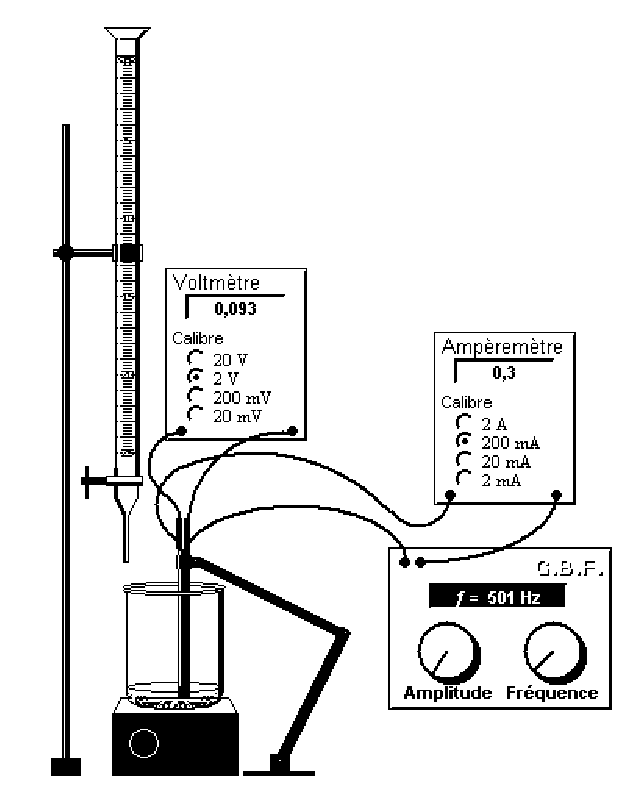
\includegraphics[width=6cm]{tp_prem_s_chimie/tp6_determination_par_conductimetrie_concentration/montage_conductimetrie.png.eps}
\caption{Dispositif exp�rimental}
\end{figure}
\end{center}


\end{multicols}



\subsection{R�sultats}
\begin{enumerate}
\item Calculer la conductance $G$ et compl�ter le tableau suivant.

\begin{arraydata}{6}
\hline
$V_0$ ($mL$)       &  0 &  5 & 10 & 15 & 20 & 25 \\ \hline
\rule[-0.4cm]{0cm}{1cm}
$C$ ($mol.L^{-1}$) &    &    &    &    &    &    \\ \hline
\rule[-0.4cm]{0cm}{1cm}
$G$ ($mS$)         &    &    &    &    &    &    \\ \hline
\end{arraydata}

\item Tracer la courbe d'�talonnage $G = f (C)$.
\end{enumerate}



\pagebreak
%\newpage


\section{D�termination de la concentration en $NaCl$ d'une solution de
  s�rum physiologique}

L'objectif est de d�terminer la concentration du chlorure de sodium dans le s�rum physiologique injectable.

\begin{enumerate}
\item Diluer au $1/100\ieme$ le s�rum physiologique. En pr�parer $500~mL$.

\item D�crire � l'aide de sch�mas le protocole utilis� pour r�aliser
  cette dilution au $1/100\ieme$ et obtenir la solution $S'$.

\item D�terminer la conductance $G'$ de cette solution $S'$.

\item En d�duire la concentration $C'$ du chlorure de sodium dans le
  s�rum physiologique dilu�.

\end{enumerate}


\vressort{3}

\section{Questions compl�mentaires}

%\begin{multicols}{2}

\begin{enumerate}
\item Expliquer comment calculer la concentration $C$ des diff�rentes
  solutions de chlorure de sodium. Donner l'expression de $C$ en
  fonction de $C_0$, $V_0$, $V$.


\item Comment calcule-t-on la conductance $G$ ?

\item Pour quelle raison pratique a-t-on int�r�t � prendre $U =
  1,00~V$ dans les diff�rentes manipulations ?

\item En extrapolant la courbe d'�talonnage, pr�voir la conductance
  d'une portion de solution concentr�e � $T = 58,4~g.L^{-1}$. Mesurer
  la conductance r�elle d'une portion d'une telle solution. Que
  peut-on conclure quant � la m�thode d'�talonnage utilis�e. On donne
  $M_{Na} = 23~g.mol^{-1}$ et $M_{Cl} = 35,5~g.mol^{-1}$.

\item Rappeler la valeur de la concentration $C'$ du chlorure de
  sodium dans le s�rum physiologique dilu�.

\item Comment peut-on alors d�terminer la concentration $C_0'$ du
  chlorure de sodium dans la solution commerciale de s�rum
  physiologique ? Calculer cette concentration $C_0'$ puis le titre
  massique (concentration massique) correspondant $T_0$. Le comparer avec
  les indications figurant sur l'�tiquette du flacon ($0,9~\%$ en masse).
\end{enumerate}


%\vressort{1}
\vressort{3}

\begin{center}
\begin{figure}[H]
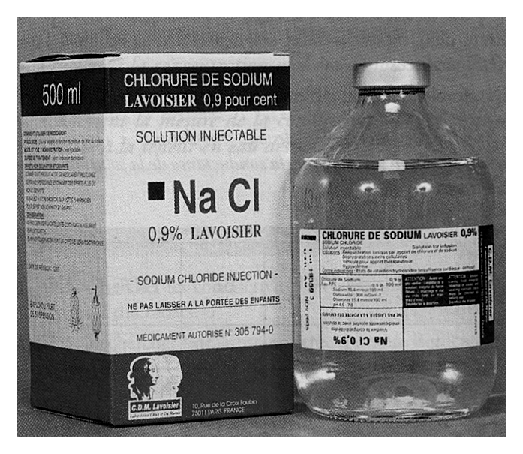
\includegraphics[width=7cm]{tp_prem_s_chimie/tp6_determination_par_conductimetrie_concentration/solution_nacl.png.eps}
\caption{Solution de chlorure de sodium}
\end{figure}
\end{center}


%\end{multicols}


\vressort{3} % cours elec circuit �lectrique

\tp{D�termination par conductim�trie\\
de la concentration en solut�\\
d'une solution ionique}


\begin{multicols}{2}

\objectifs{
\item r�aliser une courbe d'�talonnage $G = f(C)$ et en d�duire une
  concentration inconnue.
\item Aborder une limite de la m�thode d'�talonnage.
}
\vspace*{2cm}


\materiel{
\item b�cher $600~mL$
\item fiole jaug�e $500~mL$
\item burette gradu�e $25~mL$
\item pipette jaug�e $5~mL$
\item agitateur magn�tique.
\item solution de chlorure de sodium $S_0$ de concentration $C_0 =
  0,10~mol.L^{-1}$
\item flacon de s�rum physiologique
\item eau d�min�ralis�e
\item g�n�rateur basse fr�quence.
\item 2 multim�tres
\item cellule de conductim�trie.
}


\end{multicols}




\section{R�alisation d'une �chelle de conductance}


\begin{multicols}{2}

\subsection{Protocole op�ratoire}
\begin{enumerate}
\item Rincer la burette, la remplir � l'aide de la solution $S_0$ ajuster le
z�ro.

\item Avec la fiole jaug�e, introduire $V = 500~mL$ d'eau d�min�ralis�e dans
le b�cher.

\item Placer la cellule conductim�trique dans le b�cher et r�aliser le
montage �lectrique correspondant au sch�ma ci-contre. Les 2
multim�tres sont en mode alternatif ($AC$ ou \acsymbol).

\item Sur le GBF, r�gler la fr�quence $500~Hz$ et fixer la tension �
$1,00~V$.

\item Au contenu du b�cher, ajouter les volumes $V_0$ suivants de solution
de chlorure de sodium mesur�s pr�cis�ment gr�ce � la burette. Apr�s
chaque addition, v�rifier que la tension est toujours de $1,00~V$ et
relever la valeur de l'intensit�.

\end{enumerate}




\begin{center}
\begin{figure}[H]
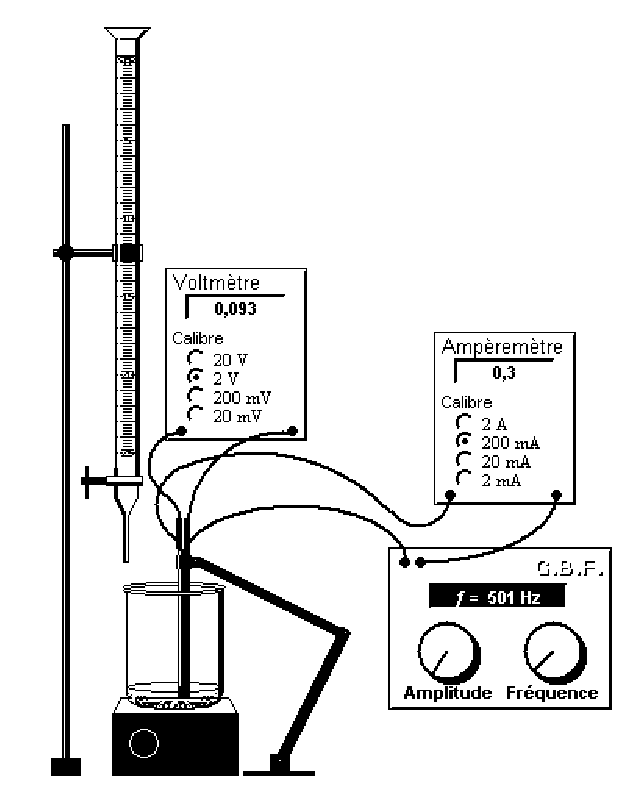
\includegraphics[width=6cm]{tp_prem_s_chimie/tp6_determination_par_conductimetrie_concentration/montage_conductimetrie.png.eps}
\caption{Dispositif exp�rimental}
\end{figure}
\end{center}


\end{multicols}



\subsection{R�sultats}
\begin{enumerate}
\item Calculer la conductance $G$ et compl�ter le tableau suivant.

\begin{arraydata}{6}
\hline
$V_0$ ($mL$)       &  0 &  5 & 10 & 15 & 20 & 25 \\ \hline
\rule[-0.4cm]{0cm}{1cm}
$C$ ($mol.L^{-1}$) &    &    &    &    &    &    \\ \hline
\rule[-0.4cm]{0cm}{1cm}
$G$ ($mS$)         &    &    &    &    &    &    \\ \hline
\end{arraydata}

\item Tracer la courbe d'�talonnage $G = f (C)$.
\end{enumerate}



\pagebreak
%\newpage


\section{D�termination de la concentration en $NaCl$ d'une solution de
  s�rum physiologique}

L'objectif est de d�terminer la concentration du chlorure de sodium dans le s�rum physiologique injectable.

\begin{enumerate}
\item Diluer au $1/100\ieme$ le s�rum physiologique. En pr�parer $500~mL$.

\item D�crire � l'aide de sch�mas le protocole utilis� pour r�aliser
  cette dilution au $1/100\ieme$ et obtenir la solution $S'$.

\item D�terminer la conductance $G'$ de cette solution $S'$.

\item En d�duire la concentration $C'$ du chlorure de sodium dans le
  s�rum physiologique dilu�.

\end{enumerate}


\vressort{3}

\section{Questions compl�mentaires}

%\begin{multicols}{2}

\begin{enumerate}
\item Expliquer comment calculer la concentration $C$ des diff�rentes
  solutions de chlorure de sodium. Donner l'expression de $C$ en
  fonction de $C_0$, $V_0$, $V$.


\item Comment calcule-t-on la conductance $G$ ?

\item Pour quelle raison pratique a-t-on int�r�t � prendre $U =
  1,00~V$ dans les diff�rentes manipulations ?

\item En extrapolant la courbe d'�talonnage, pr�voir la conductance
  d'une portion de solution concentr�e � $T = 58,4~g.L^{-1}$. Mesurer
  la conductance r�elle d'une portion d'une telle solution. Que
  peut-on conclure quant � la m�thode d'�talonnage utilis�e. On donne
  $M_{Na} = 23~g.mol^{-1}$ et $M_{Cl} = 35,5~g.mol^{-1}$.

\item Rappeler la valeur de la concentration $C'$ du chlorure de
  sodium dans le s�rum physiologique dilu�.

\item Comment peut-on alors d�terminer la concentration $C_0'$ du
  chlorure de sodium dans la solution commerciale de s�rum
  physiologique ? Calculer cette concentration $C_0'$ puis le titre
  massique (concentration massique) correspondant $T_0$. Le comparer avec
  les indications figurant sur l'�tiquette du flacon ($0,9~\%$ en masse).
\end{enumerate}


%\vressort{1}
\vressort{3}

\begin{center}
\begin{figure}[H]
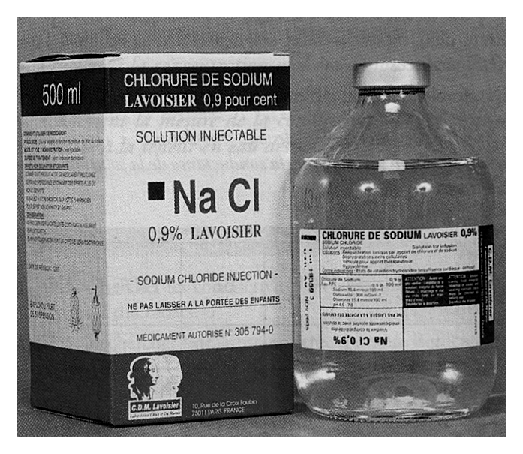
\includegraphics[width=7cm]{tp_prem_s_chimie/tp6_determination_par_conductimetrie_concentration/solution_nacl.png.eps}
\caption{Solution de chlorure de sodium}
\end{figure}
\end{center}


%\end{multicols}


\vressort{3} % tp mesure de tension et d'intensit�

\tp{D�termination par conductim�trie\\
de la concentration en solut�\\
d'une solution ionique}


\begin{multicols}{2}

\objectifs{
\item r�aliser une courbe d'�talonnage $G = f(C)$ et en d�duire une
  concentration inconnue.
\item Aborder une limite de la m�thode d'�talonnage.
}
\vspace*{2cm}


\materiel{
\item b�cher $600~mL$
\item fiole jaug�e $500~mL$
\item burette gradu�e $25~mL$
\item pipette jaug�e $5~mL$
\item agitateur magn�tique.
\item solution de chlorure de sodium $S_0$ de concentration $C_0 =
  0,10~mol.L^{-1}$
\item flacon de s�rum physiologique
\item eau d�min�ralis�e
\item g�n�rateur basse fr�quence.
\item 2 multim�tres
\item cellule de conductim�trie.
}


\end{multicols}




\section{R�alisation d'une �chelle de conductance}


\begin{multicols}{2}

\subsection{Protocole op�ratoire}
\begin{enumerate}
\item Rincer la burette, la remplir � l'aide de la solution $S_0$ ajuster le
z�ro.

\item Avec la fiole jaug�e, introduire $V = 500~mL$ d'eau d�min�ralis�e dans
le b�cher.

\item Placer la cellule conductim�trique dans le b�cher et r�aliser le
montage �lectrique correspondant au sch�ma ci-contre. Les 2
multim�tres sont en mode alternatif ($AC$ ou \acsymbol).

\item Sur le GBF, r�gler la fr�quence $500~Hz$ et fixer la tension �
$1,00~V$.

\item Au contenu du b�cher, ajouter les volumes $V_0$ suivants de solution
de chlorure de sodium mesur�s pr�cis�ment gr�ce � la burette. Apr�s
chaque addition, v�rifier que la tension est toujours de $1,00~V$ et
relever la valeur de l'intensit�.

\end{enumerate}




\begin{center}
\begin{figure}[H]
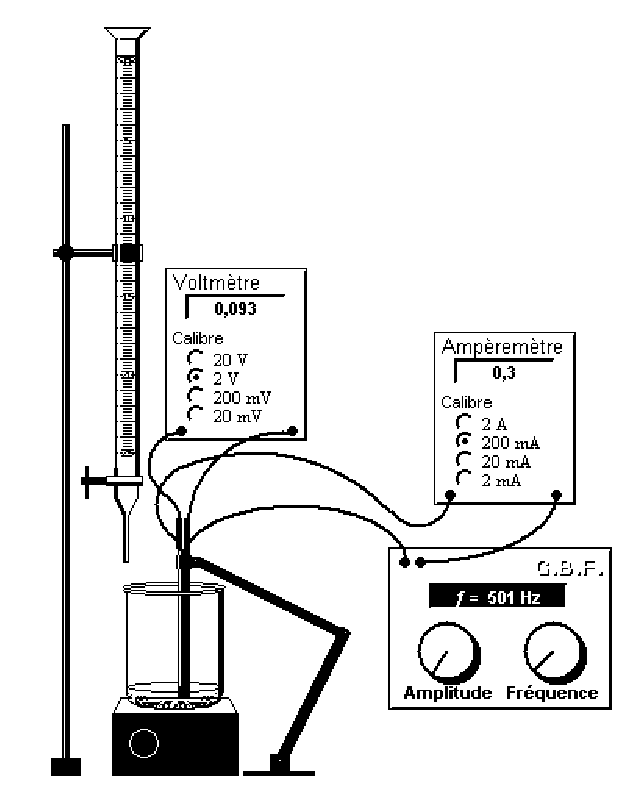
\includegraphics[width=6cm]{tp_prem_s_chimie/tp6_determination_par_conductimetrie_concentration/montage_conductimetrie.png.eps}
\caption{Dispositif exp�rimental}
\end{figure}
\end{center}


\end{multicols}



\subsection{R�sultats}
\begin{enumerate}
\item Calculer la conductance $G$ et compl�ter le tableau suivant.

\begin{arraydata}{6}
\hline
$V_0$ ($mL$)       &  0 &  5 & 10 & 15 & 20 & 25 \\ \hline
\rule[-0.4cm]{0cm}{1cm}
$C$ ($mol.L^{-1}$) &    &    &    &    &    &    \\ \hline
\rule[-0.4cm]{0cm}{1cm}
$G$ ($mS$)         &    &    &    &    &    &    \\ \hline
\end{arraydata}

\item Tracer la courbe d'�talonnage $G = f (C)$.
\end{enumerate}



\pagebreak
%\newpage


\section{D�termination de la concentration en $NaCl$ d'une solution de
  s�rum physiologique}

L'objectif est de d�terminer la concentration du chlorure de sodium dans le s�rum physiologique injectable.

\begin{enumerate}
\item Diluer au $1/100\ieme$ le s�rum physiologique. En pr�parer $500~mL$.

\item D�crire � l'aide de sch�mas le protocole utilis� pour r�aliser
  cette dilution au $1/100\ieme$ et obtenir la solution $S'$.

\item D�terminer la conductance $G'$ de cette solution $S'$.

\item En d�duire la concentration $C'$ du chlorure de sodium dans le
  s�rum physiologique dilu�.

\end{enumerate}


\vressort{3}

\section{Questions compl�mentaires}

%\begin{multicols}{2}

\begin{enumerate}
\item Expliquer comment calculer la concentration $C$ des diff�rentes
  solutions de chlorure de sodium. Donner l'expression de $C$ en
  fonction de $C_0$, $V_0$, $V$.


\item Comment calcule-t-on la conductance $G$ ?

\item Pour quelle raison pratique a-t-on int�r�t � prendre $U =
  1,00~V$ dans les diff�rentes manipulations ?

\item En extrapolant la courbe d'�talonnage, pr�voir la conductance
  d'une portion de solution concentr�e � $T = 58,4~g.L^{-1}$. Mesurer
  la conductance r�elle d'une portion d'une telle solution. Que
  peut-on conclure quant � la m�thode d'�talonnage utilis�e. On donne
  $M_{Na} = 23~g.mol^{-1}$ et $M_{Cl} = 35,5~g.mol^{-1}$.

\item Rappeler la valeur de la concentration $C'$ du chlorure de
  sodium dans le s�rum physiologique dilu�.

\item Comment peut-on alors d�terminer la concentration $C_0'$ du
  chlorure de sodium dans la solution commerciale de s�rum
  physiologique ? Calculer cette concentration $C_0'$ puis le titre
  massique (concentration massique) correspondant $T_0$. Le comparer avec
  les indications figurant sur l'�tiquette du flacon ($0,9~\%$ en masse).
\end{enumerate}


%\vressort{1}
\vressort{3}

\begin{center}
\begin{figure}[H]
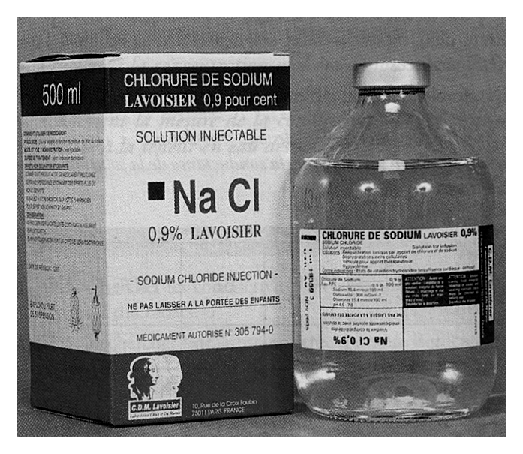
\includegraphics[width=7cm]{tp_prem_s_chimie/tp6_determination_par_conductimetrie_concentration/solution_nacl.png.eps}
\caption{Solution de chlorure de sodium}
\end{figure}
\end{center}


%\end{multicols}


\vressort{3} % document fiche
    % m�thode montage
    % utilisation d'un multim�tre, ...

\tp{D�termination par conductim�trie\\
de la concentration en solut�\\
d'une solution ionique}


\begin{multicols}{2}

\objectifs{
\item r�aliser une courbe d'�talonnage $G = f(C)$ et en d�duire une
  concentration inconnue.
\item Aborder une limite de la m�thode d'�talonnage.
}
\vspace*{2cm}


\materiel{
\item b�cher $600~mL$
\item fiole jaug�e $500~mL$
\item burette gradu�e $25~mL$
\item pipette jaug�e $5~mL$
\item agitateur magn�tique.
\item solution de chlorure de sodium $S_0$ de concentration $C_0 =
  0,10~mol.L^{-1}$
\item flacon de s�rum physiologique
\item eau d�min�ralis�e
\item g�n�rateur basse fr�quence.
\item 2 multim�tres
\item cellule de conductim�trie.
}


\end{multicols}




\section{R�alisation d'une �chelle de conductance}


\begin{multicols}{2}

\subsection{Protocole op�ratoire}
\begin{enumerate}
\item Rincer la burette, la remplir � l'aide de la solution $S_0$ ajuster le
z�ro.

\item Avec la fiole jaug�e, introduire $V = 500~mL$ d'eau d�min�ralis�e dans
le b�cher.

\item Placer la cellule conductim�trique dans le b�cher et r�aliser le
montage �lectrique correspondant au sch�ma ci-contre. Les 2
multim�tres sont en mode alternatif ($AC$ ou \acsymbol).

\item Sur le GBF, r�gler la fr�quence $500~Hz$ et fixer la tension �
$1,00~V$.

\item Au contenu du b�cher, ajouter les volumes $V_0$ suivants de solution
de chlorure de sodium mesur�s pr�cis�ment gr�ce � la burette. Apr�s
chaque addition, v�rifier que la tension est toujours de $1,00~V$ et
relever la valeur de l'intensit�.

\end{enumerate}




\begin{center}
\begin{figure}[H]
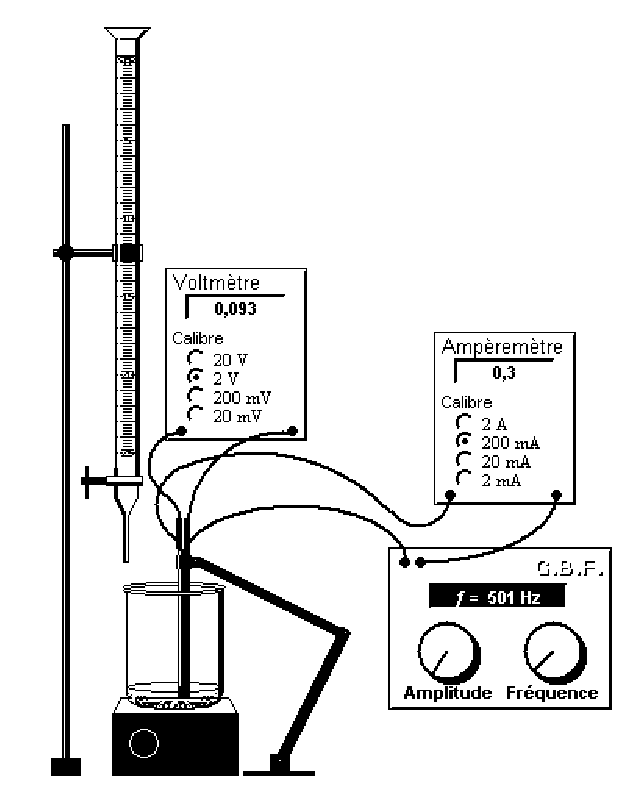
\includegraphics[width=6cm]{tp_prem_s_chimie/tp6_determination_par_conductimetrie_concentration/montage_conductimetrie.png.eps}
\caption{Dispositif exp�rimental}
\end{figure}
\end{center}


\end{multicols}



\subsection{R�sultats}
\begin{enumerate}
\item Calculer la conductance $G$ et compl�ter le tableau suivant.

\begin{arraydata}{6}
\hline
$V_0$ ($mL$)       &  0 &  5 & 10 & 15 & 20 & 25 \\ \hline
\rule[-0.4cm]{0cm}{1cm}
$C$ ($mol.L^{-1}$) &    &    &    &    &    &    \\ \hline
\rule[-0.4cm]{0cm}{1cm}
$G$ ($mS$)         &    &    &    &    &    &    \\ \hline
\end{arraydata}

\item Tracer la courbe d'�talonnage $G = f (C)$.
\end{enumerate}



\pagebreak
%\newpage


\section{D�termination de la concentration en $NaCl$ d'une solution de
  s�rum physiologique}

L'objectif est de d�terminer la concentration du chlorure de sodium dans le s�rum physiologique injectable.

\begin{enumerate}
\item Diluer au $1/100\ieme$ le s�rum physiologique. En pr�parer $500~mL$.

\item D�crire � l'aide de sch�mas le protocole utilis� pour r�aliser
  cette dilution au $1/100\ieme$ et obtenir la solution $S'$.

\item D�terminer la conductance $G'$ de cette solution $S'$.

\item En d�duire la concentration $C'$ du chlorure de sodium dans le
  s�rum physiologique dilu�.

\end{enumerate}


\vressort{3}

\section{Questions compl�mentaires}

%\begin{multicols}{2}

\begin{enumerate}
\item Expliquer comment calculer la concentration $C$ des diff�rentes
  solutions de chlorure de sodium. Donner l'expression de $C$ en
  fonction de $C_0$, $V_0$, $V$.


\item Comment calcule-t-on la conductance $G$ ?

\item Pour quelle raison pratique a-t-on int�r�t � prendre $U =
  1,00~V$ dans les diff�rentes manipulations ?

\item En extrapolant la courbe d'�talonnage, pr�voir la conductance
  d'une portion de solution concentr�e � $T = 58,4~g.L^{-1}$. Mesurer
  la conductance r�elle d'une portion d'une telle solution. Que
  peut-on conclure quant � la m�thode d'�talonnage utilis�e. On donne
  $M_{Na} = 23~g.mol^{-1}$ et $M_{Cl} = 35,5~g.mol^{-1}$.

\item Rappeler la valeur de la concentration $C'$ du chlorure de
  sodium dans le s�rum physiologique dilu�.

\item Comment peut-on alors d�terminer la concentration $C_0'$ du
  chlorure de sodium dans la solution commerciale de s�rum
  physiologique ? Calculer cette concentration $C_0'$ puis le titre
  massique (concentration massique) correspondant $T_0$. Le comparer avec
  les indications figurant sur l'�tiquette du flacon ($0,9~\%$ en masse).
\end{enumerate}


%\vressort{1}
\vressort{3}

\begin{center}
\begin{figure}[H]
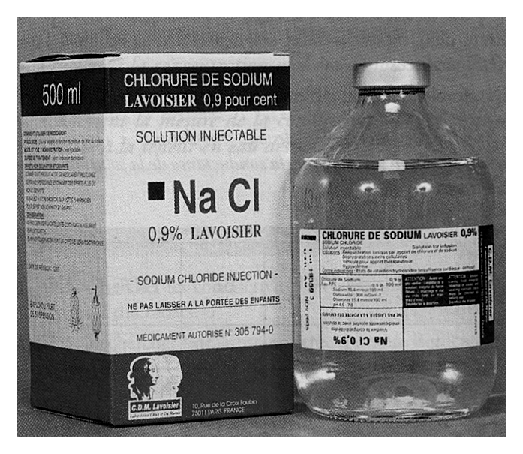
\includegraphics[width=7cm]{tp_prem_s_chimie/tp6_determination_par_conductimetrie_concentration/solution_nacl.png.eps}
\caption{Solution de chlorure de sodium}
\end{figure}
\end{center}


%\end{multicols}


\vressort{3} % tp loi d'ohm

\tp{D�termination par conductim�trie\\
de la concentration en solut�\\
d'une solution ionique}


\begin{multicols}{2}

\objectifs{
\item r�aliser une courbe d'�talonnage $G = f(C)$ et en d�duire une
  concentration inconnue.
\item Aborder une limite de la m�thode d'�talonnage.
}
\vspace*{2cm}


\materiel{
\item b�cher $600~mL$
\item fiole jaug�e $500~mL$
\item burette gradu�e $25~mL$
\item pipette jaug�e $5~mL$
\item agitateur magn�tique.
\item solution de chlorure de sodium $S_0$ de concentration $C_0 =
  0,10~mol.L^{-1}$
\item flacon de s�rum physiologique
\item eau d�min�ralis�e
\item g�n�rateur basse fr�quence.
\item 2 multim�tres
\item cellule de conductim�trie.
}


\end{multicols}




\section{R�alisation d'une �chelle de conductance}


\begin{multicols}{2}

\subsection{Protocole op�ratoire}
\begin{enumerate}
\item Rincer la burette, la remplir � l'aide de la solution $S_0$ ajuster le
z�ro.

\item Avec la fiole jaug�e, introduire $V = 500~mL$ d'eau d�min�ralis�e dans
le b�cher.

\item Placer la cellule conductim�trique dans le b�cher et r�aliser le
montage �lectrique correspondant au sch�ma ci-contre. Les 2
multim�tres sont en mode alternatif ($AC$ ou \acsymbol).

\item Sur le GBF, r�gler la fr�quence $500~Hz$ et fixer la tension �
$1,00~V$.

\item Au contenu du b�cher, ajouter les volumes $V_0$ suivants de solution
de chlorure de sodium mesur�s pr�cis�ment gr�ce � la burette. Apr�s
chaque addition, v�rifier que la tension est toujours de $1,00~V$ et
relever la valeur de l'intensit�.

\end{enumerate}




\begin{center}
\begin{figure}[H]
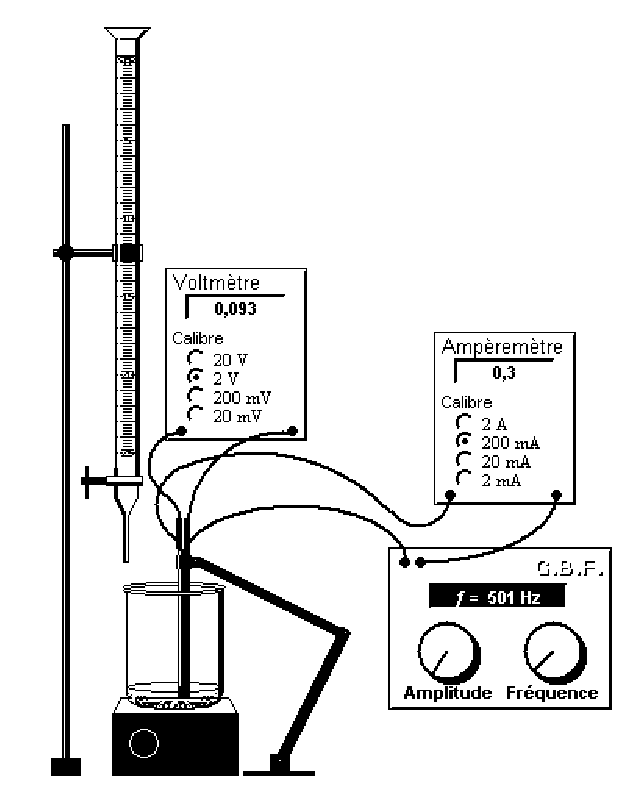
\includegraphics[width=6cm]{tp_prem_s_chimie/tp6_determination_par_conductimetrie_concentration/montage_conductimetrie.png.eps}
\caption{Dispositif exp�rimental}
\end{figure}
\end{center}


\end{multicols}



\subsection{R�sultats}
\begin{enumerate}
\item Calculer la conductance $G$ et compl�ter le tableau suivant.

\begin{arraydata}{6}
\hline
$V_0$ ($mL$)       &  0 &  5 & 10 & 15 & 20 & 25 \\ \hline
\rule[-0.4cm]{0cm}{1cm}
$C$ ($mol.L^{-1}$) &    &    &    &    &    &    \\ \hline
\rule[-0.4cm]{0cm}{1cm}
$G$ ($mS$)         &    &    &    &    &    &    \\ \hline
\end{arraydata}

\item Tracer la courbe d'�talonnage $G = f (C)$.
\end{enumerate}



\pagebreak
%\newpage


\section{D�termination de la concentration en $NaCl$ d'une solution de
  s�rum physiologique}

L'objectif est de d�terminer la concentration du chlorure de sodium dans le s�rum physiologique injectable.

\begin{enumerate}
\item Diluer au $1/100\ieme$ le s�rum physiologique. En pr�parer $500~mL$.

\item D�crire � l'aide de sch�mas le protocole utilis� pour r�aliser
  cette dilution au $1/100\ieme$ et obtenir la solution $S'$.

\item D�terminer la conductance $G'$ de cette solution $S'$.

\item En d�duire la concentration $C'$ du chlorure de sodium dans le
  s�rum physiologique dilu�.

\end{enumerate}


\vressort{3}

\section{Questions compl�mentaires}

%\begin{multicols}{2}

\begin{enumerate}
\item Expliquer comment calculer la concentration $C$ des diff�rentes
  solutions de chlorure de sodium. Donner l'expression de $C$ en
  fonction de $C_0$, $V_0$, $V$.


\item Comment calcule-t-on la conductance $G$ ?

\item Pour quelle raison pratique a-t-on int�r�t � prendre $U =
  1,00~V$ dans les diff�rentes manipulations ?

\item En extrapolant la courbe d'�talonnage, pr�voir la conductance
  d'une portion de solution concentr�e � $T = 58,4~g.L^{-1}$. Mesurer
  la conductance r�elle d'une portion d'une telle solution. Que
  peut-on conclure quant � la m�thode d'�talonnage utilis�e. On donne
  $M_{Na} = 23~g.mol^{-1}$ et $M_{Cl} = 35,5~g.mol^{-1}$.

\item Rappeler la valeur de la concentration $C'$ du chlorure de
  sodium dans le s�rum physiologique dilu�.

\item Comment peut-on alors d�terminer la concentration $C_0'$ du
  chlorure de sodium dans la solution commerciale de s�rum
  physiologique ? Calculer cette concentration $C_0'$ puis le titre
  massique (concentration massique) correspondant $T_0$. Le comparer avec
  les indications figurant sur l'�tiquette du flacon ($0,9~\%$ en masse).
\end{enumerate}


%\vressort{1}
\vressort{3}

\begin{center}
\begin{figure}[H]
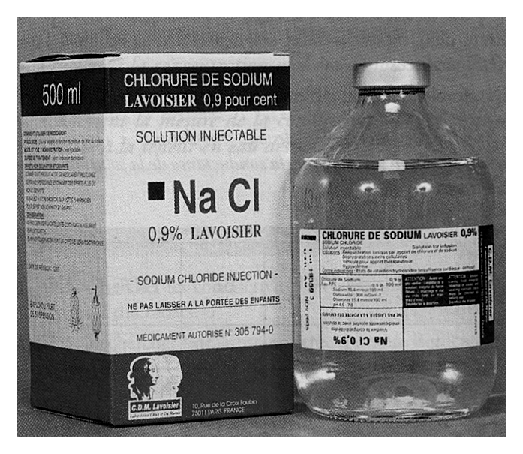
\includegraphics[width=7cm]{tp_prem_s_chimie/tp6_determination_par_conductimetrie_concentration/solution_nacl.png.eps}
\caption{Solution de chlorure de sodium}
\end{figure}
\end{center}


%\end{multicols}


\vressort{3} % tp associations de R

% association r s�rie (trac� U en fonction de I et montrer qu'on ajoute U)
% association r parall�le (trac� U en fonction de I et montrer qu'on ajoute I)



\chapitre{G�n�rateurs et r�cepteurs}
\tp{D�termination par conductim�trie\\
de la concentration en solut�\\
d'une solution ionique}


\begin{multicols}{2}

\objectifs{
\item r�aliser une courbe d'�talonnage $G = f(C)$ et en d�duire une
  concentration inconnue.
\item Aborder une limite de la m�thode d'�talonnage.
}
\vspace*{2cm}


\materiel{
\item b�cher $600~mL$
\item fiole jaug�e $500~mL$
\item burette gradu�e $25~mL$
\item pipette jaug�e $5~mL$
\item agitateur magn�tique.
\item solution de chlorure de sodium $S_0$ de concentration $C_0 =
  0,10~mol.L^{-1}$
\item flacon de s�rum physiologique
\item eau d�min�ralis�e
\item g�n�rateur basse fr�quence.
\item 2 multim�tres
\item cellule de conductim�trie.
}


\end{multicols}




\section{R�alisation d'une �chelle de conductance}


\begin{multicols}{2}

\subsection{Protocole op�ratoire}
\begin{enumerate}
\item Rincer la burette, la remplir � l'aide de la solution $S_0$ ajuster le
z�ro.

\item Avec la fiole jaug�e, introduire $V = 500~mL$ d'eau d�min�ralis�e dans
le b�cher.

\item Placer la cellule conductim�trique dans le b�cher et r�aliser le
montage �lectrique correspondant au sch�ma ci-contre. Les 2
multim�tres sont en mode alternatif ($AC$ ou \acsymbol).

\item Sur le GBF, r�gler la fr�quence $500~Hz$ et fixer la tension �
$1,00~V$.

\item Au contenu du b�cher, ajouter les volumes $V_0$ suivants de solution
de chlorure de sodium mesur�s pr�cis�ment gr�ce � la burette. Apr�s
chaque addition, v�rifier que la tension est toujours de $1,00~V$ et
relever la valeur de l'intensit�.

\end{enumerate}




\begin{center}
\begin{figure}[H]
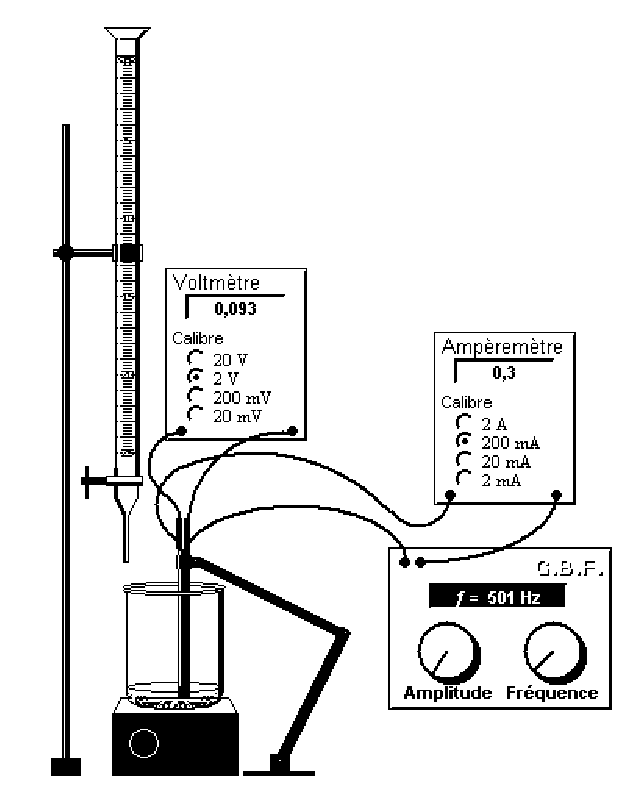
\includegraphics[width=6cm]{tp_prem_s_chimie/tp6_determination_par_conductimetrie_concentration/montage_conductimetrie.png.eps}
\caption{Dispositif exp�rimental}
\end{figure}
\end{center}


\end{multicols}



\subsection{R�sultats}
\begin{enumerate}
\item Calculer la conductance $G$ et compl�ter le tableau suivant.

\begin{arraydata}{6}
\hline
$V_0$ ($mL$)       &  0 &  5 & 10 & 15 & 20 & 25 \\ \hline
\rule[-0.4cm]{0cm}{1cm}
$C$ ($mol.L^{-1}$) &    &    &    &    &    &    \\ \hline
\rule[-0.4cm]{0cm}{1cm}
$G$ ($mS$)         &    &    &    &    &    &    \\ \hline
\end{arraydata}

\item Tracer la courbe d'�talonnage $G = f (C)$.
\end{enumerate}



\pagebreak
%\newpage


\section{D�termination de la concentration en $NaCl$ d'une solution de
  s�rum physiologique}

L'objectif est de d�terminer la concentration du chlorure de sodium dans le s�rum physiologique injectable.

\begin{enumerate}
\item Diluer au $1/100\ieme$ le s�rum physiologique. En pr�parer $500~mL$.

\item D�crire � l'aide de sch�mas le protocole utilis� pour r�aliser
  cette dilution au $1/100\ieme$ et obtenir la solution $S'$.

\item D�terminer la conductance $G'$ de cette solution $S'$.

\item En d�duire la concentration $C'$ du chlorure de sodium dans le
  s�rum physiologique dilu�.

\end{enumerate}


\vressort{3}

\section{Questions compl�mentaires}

%\begin{multicols}{2}

\begin{enumerate}
\item Expliquer comment calculer la concentration $C$ des diff�rentes
  solutions de chlorure de sodium. Donner l'expression de $C$ en
  fonction de $C_0$, $V_0$, $V$.


\item Comment calcule-t-on la conductance $G$ ?

\item Pour quelle raison pratique a-t-on int�r�t � prendre $U =
  1,00~V$ dans les diff�rentes manipulations ?

\item En extrapolant la courbe d'�talonnage, pr�voir la conductance
  d'une portion de solution concentr�e � $T = 58,4~g.L^{-1}$. Mesurer
  la conductance r�elle d'une portion d'une telle solution. Que
  peut-on conclure quant � la m�thode d'�talonnage utilis�e. On donne
  $M_{Na} = 23~g.mol^{-1}$ et $M_{Cl} = 35,5~g.mol^{-1}$.

\item Rappeler la valeur de la concentration $C'$ du chlorure de
  sodium dans le s�rum physiologique dilu�.

\item Comment peut-on alors d�terminer la concentration $C_0'$ du
  chlorure de sodium dans la solution commerciale de s�rum
  physiologique ? Calculer cette concentration $C_0'$ puis le titre
  massique (concentration massique) correspondant $T_0$. Le comparer avec
  les indications figurant sur l'�tiquette du flacon ($0,9~\%$ en masse).
\end{enumerate}


%\vressort{1}
\vressort{3}

\begin{center}
\begin{figure}[H]
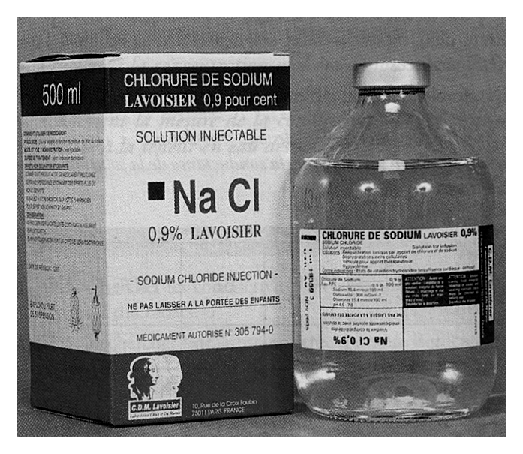
\includegraphics[width=7cm]{tp_prem_s_chimie/tp6_determination_par_conductimetrie_concentration/solution_nacl.png.eps}
\caption{Solution de chlorure de sodium}
\end{figure}
\end{center}


%\end{multicols}


\vressort{3} % cours elec g�n�rateurs, r�cepteurs

\tp{D�termination par conductim�trie\\
de la concentration en solut�\\
d'une solution ionique}


\begin{multicols}{2}

\objectifs{
\item r�aliser une courbe d'�talonnage $G = f(C)$ et en d�duire une
  concentration inconnue.
\item Aborder une limite de la m�thode d'�talonnage.
}
\vspace*{2cm}


\materiel{
\item b�cher $600~mL$
\item fiole jaug�e $500~mL$
\item burette gradu�e $25~mL$
\item pipette jaug�e $5~mL$
\item agitateur magn�tique.
\item solution de chlorure de sodium $S_0$ de concentration $C_0 =
  0,10~mol.L^{-1}$
\item flacon de s�rum physiologique
\item eau d�min�ralis�e
\item g�n�rateur basse fr�quence.
\item 2 multim�tres
\item cellule de conductim�trie.
}


\end{multicols}




\section{R�alisation d'une �chelle de conductance}


\begin{multicols}{2}

\subsection{Protocole op�ratoire}
\begin{enumerate}
\item Rincer la burette, la remplir � l'aide de la solution $S_0$ ajuster le
z�ro.

\item Avec la fiole jaug�e, introduire $V = 500~mL$ d'eau d�min�ralis�e dans
le b�cher.

\item Placer la cellule conductim�trique dans le b�cher et r�aliser le
montage �lectrique correspondant au sch�ma ci-contre. Les 2
multim�tres sont en mode alternatif ($AC$ ou \acsymbol).

\item Sur le GBF, r�gler la fr�quence $500~Hz$ et fixer la tension �
$1,00~V$.

\item Au contenu du b�cher, ajouter les volumes $V_0$ suivants de solution
de chlorure de sodium mesur�s pr�cis�ment gr�ce � la burette. Apr�s
chaque addition, v�rifier que la tension est toujours de $1,00~V$ et
relever la valeur de l'intensit�.

\end{enumerate}




\begin{center}
\begin{figure}[H]
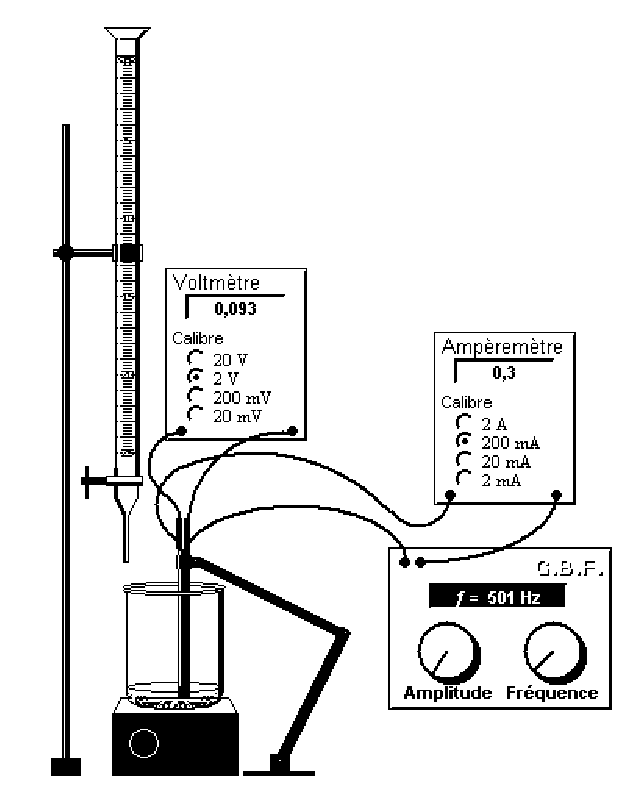
\includegraphics[width=6cm]{tp_prem_s_chimie/tp6_determination_par_conductimetrie_concentration/montage_conductimetrie.png.eps}
\caption{Dispositif exp�rimental}
\end{figure}
\end{center}


\end{multicols}



\subsection{R�sultats}
\begin{enumerate}
\item Calculer la conductance $G$ et compl�ter le tableau suivant.

\begin{arraydata}{6}
\hline
$V_0$ ($mL$)       &  0 &  5 & 10 & 15 & 20 & 25 \\ \hline
\rule[-0.4cm]{0cm}{1cm}
$C$ ($mol.L^{-1}$) &    &    &    &    &    &    \\ \hline
\rule[-0.4cm]{0cm}{1cm}
$G$ ($mS$)         &    &    &    &    &    &    \\ \hline
\end{arraydata}

\item Tracer la courbe d'�talonnage $G = f (C)$.
\end{enumerate}



\pagebreak
%\newpage


\section{D�termination de la concentration en $NaCl$ d'une solution de
  s�rum physiologique}

L'objectif est de d�terminer la concentration du chlorure de sodium dans le s�rum physiologique injectable.

\begin{enumerate}
\item Diluer au $1/100\ieme$ le s�rum physiologique. En pr�parer $500~mL$.

\item D�crire � l'aide de sch�mas le protocole utilis� pour r�aliser
  cette dilution au $1/100\ieme$ et obtenir la solution $S'$.

\item D�terminer la conductance $G'$ de cette solution $S'$.

\item En d�duire la concentration $C'$ du chlorure de sodium dans le
  s�rum physiologique dilu�.

\end{enumerate}


\vressort{3}

\section{Questions compl�mentaires}

%\begin{multicols}{2}

\begin{enumerate}
\item Expliquer comment calculer la concentration $C$ des diff�rentes
  solutions de chlorure de sodium. Donner l'expression de $C$ en
  fonction de $C_0$, $V_0$, $V$.


\item Comment calcule-t-on la conductance $G$ ?

\item Pour quelle raison pratique a-t-on int�r�t � prendre $U =
  1,00~V$ dans les diff�rentes manipulations ?

\item En extrapolant la courbe d'�talonnage, pr�voir la conductance
  d'une portion de solution concentr�e � $T = 58,4~g.L^{-1}$. Mesurer
  la conductance r�elle d'une portion d'une telle solution. Que
  peut-on conclure quant � la m�thode d'�talonnage utilis�e. On donne
  $M_{Na} = 23~g.mol^{-1}$ et $M_{Cl} = 35,5~g.mol^{-1}$.

\item Rappeler la valeur de la concentration $C'$ du chlorure de
  sodium dans le s�rum physiologique dilu�.

\item Comment peut-on alors d�terminer la concentration $C_0'$ du
  chlorure de sodium dans la solution commerciale de s�rum
  physiologique ? Calculer cette concentration $C_0'$ puis le titre
  massique (concentration massique) correspondant $T_0$. Le comparer avec
  les indications figurant sur l'�tiquette du flacon ($0,9~\%$ en masse).
\end{enumerate}


%\vressort{1}
\vressort{3}

\begin{center}
\begin{figure}[H]
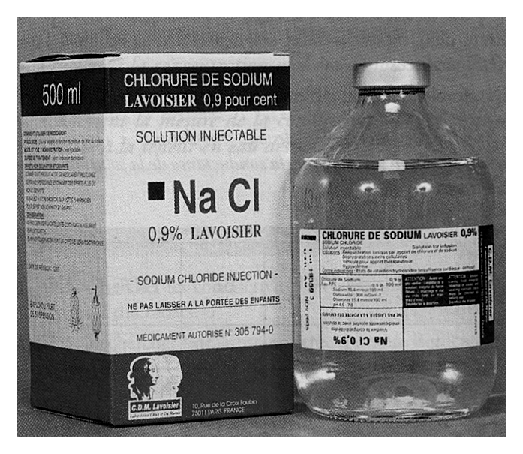
\includegraphics[width=7cm]{tp_prem_s_chimie/tp6_determination_par_conductimetrie_concentration/solution_nacl.png.eps}
\caption{Solution de chlorure de sodium}
\end{figure}
\end{center}


%\end{multicols}


\vressort{3} % tp caract�ristique d'un g�n�rateur
\tp{D�termination par conductim�trie\\
de la concentration en solut�\\
d'une solution ionique}


\begin{multicols}{2}

\objectifs{
\item r�aliser une courbe d'�talonnage $G = f(C)$ et en d�duire une
  concentration inconnue.
\item Aborder une limite de la m�thode d'�talonnage.
}
\vspace*{2cm}


\materiel{
\item b�cher $600~mL$
\item fiole jaug�e $500~mL$
\item burette gradu�e $25~mL$
\item pipette jaug�e $5~mL$
\item agitateur magn�tique.
\item solution de chlorure de sodium $S_0$ de concentration $C_0 =
  0,10~mol.L^{-1}$
\item flacon de s�rum physiologique
\item eau d�min�ralis�e
\item g�n�rateur basse fr�quence.
\item 2 multim�tres
\item cellule de conductim�trie.
}


\end{multicols}




\section{R�alisation d'une �chelle de conductance}


\begin{multicols}{2}

\subsection{Protocole op�ratoire}
\begin{enumerate}
\item Rincer la burette, la remplir � l'aide de la solution $S_0$ ajuster le
z�ro.

\item Avec la fiole jaug�e, introduire $V = 500~mL$ d'eau d�min�ralis�e dans
le b�cher.

\item Placer la cellule conductim�trique dans le b�cher et r�aliser le
montage �lectrique correspondant au sch�ma ci-contre. Les 2
multim�tres sont en mode alternatif ($AC$ ou \acsymbol).

\item Sur le GBF, r�gler la fr�quence $500~Hz$ et fixer la tension �
$1,00~V$.

\item Au contenu du b�cher, ajouter les volumes $V_0$ suivants de solution
de chlorure de sodium mesur�s pr�cis�ment gr�ce � la burette. Apr�s
chaque addition, v�rifier que la tension est toujours de $1,00~V$ et
relever la valeur de l'intensit�.

\end{enumerate}




\begin{center}
\begin{figure}[H]
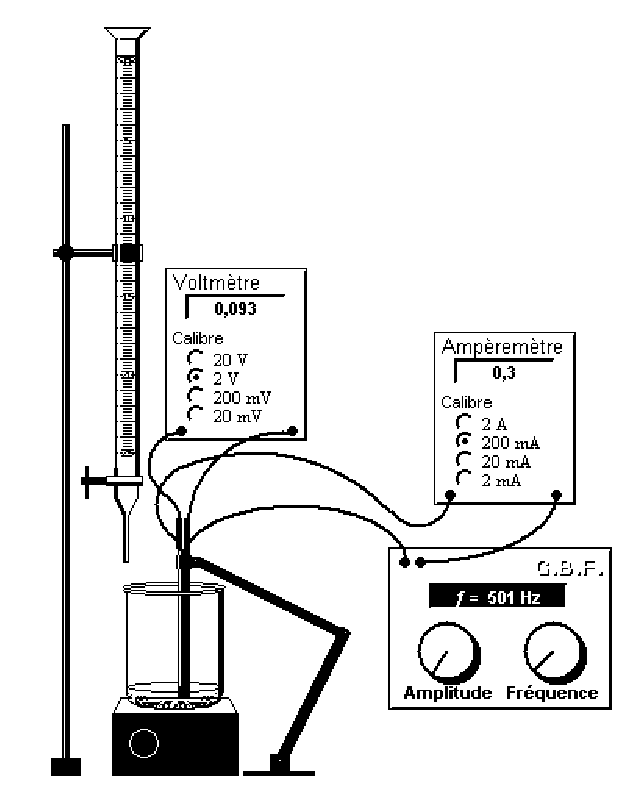
\includegraphics[width=6cm]{tp_prem_s_chimie/tp6_determination_par_conductimetrie_concentration/montage_conductimetrie.png.eps}
\caption{Dispositif exp�rimental}
\end{figure}
\end{center}


\end{multicols}



\subsection{R�sultats}
\begin{enumerate}
\item Calculer la conductance $G$ et compl�ter le tableau suivant.

\begin{arraydata}{6}
\hline
$V_0$ ($mL$)       &  0 &  5 & 10 & 15 & 20 & 25 \\ \hline
\rule[-0.4cm]{0cm}{1cm}
$C$ ($mol.L^{-1}$) &    &    &    &    &    &    \\ \hline
\rule[-0.4cm]{0cm}{1cm}
$G$ ($mS$)         &    &    &    &    &    &    \\ \hline
\end{arraydata}

\item Tracer la courbe d'�talonnage $G = f (C)$.
\end{enumerate}



\pagebreak
%\newpage


\section{D�termination de la concentration en $NaCl$ d'une solution de
  s�rum physiologique}

L'objectif est de d�terminer la concentration du chlorure de sodium dans le s�rum physiologique injectable.

\begin{enumerate}
\item Diluer au $1/100\ieme$ le s�rum physiologique. En pr�parer $500~mL$.

\item D�crire � l'aide de sch�mas le protocole utilis� pour r�aliser
  cette dilution au $1/100\ieme$ et obtenir la solution $S'$.

\item D�terminer la conductance $G'$ de cette solution $S'$.

\item En d�duire la concentration $C'$ du chlorure de sodium dans le
  s�rum physiologique dilu�.

\end{enumerate}


\vressort{3}

\section{Questions compl�mentaires}

%\begin{multicols}{2}

\begin{enumerate}
\item Expliquer comment calculer la concentration $C$ des diff�rentes
  solutions de chlorure de sodium. Donner l'expression de $C$ en
  fonction de $C_0$, $V_0$, $V$.


\item Comment calcule-t-on la conductance $G$ ?

\item Pour quelle raison pratique a-t-on int�r�t � prendre $U =
  1,00~V$ dans les diff�rentes manipulations ?

\item En extrapolant la courbe d'�talonnage, pr�voir la conductance
  d'une portion de solution concentr�e � $T = 58,4~g.L^{-1}$. Mesurer
  la conductance r�elle d'une portion d'une telle solution. Que
  peut-on conclure quant � la m�thode d'�talonnage utilis�e. On donne
  $M_{Na} = 23~g.mol^{-1}$ et $M_{Cl} = 35,5~g.mol^{-1}$.

\item Rappeler la valeur de la concentration $C'$ du chlorure de
  sodium dans le s�rum physiologique dilu�.

\item Comment peut-on alors d�terminer la concentration $C_0'$ du
  chlorure de sodium dans la solution commerciale de s�rum
  physiologique ? Calculer cette concentration $C_0'$ puis le titre
  massique (concentration massique) correspondant $T_0$. Le comparer avec
  les indications figurant sur l'�tiquette du flacon ($0,9~\%$ en masse).
\end{enumerate}


%\vressort{1}
\vressort{3}

\begin{center}
\begin{figure}[H]
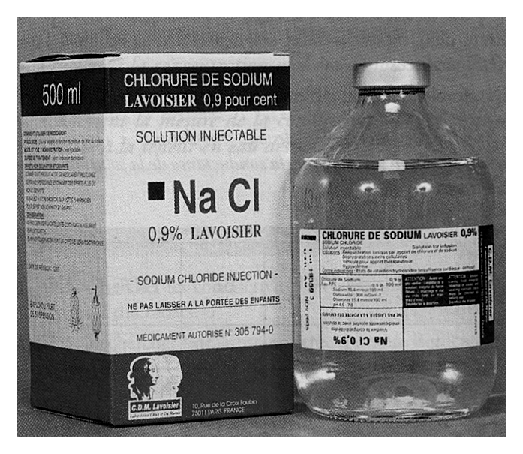
\includegraphics[width=7cm]{tp_prem_s_chimie/tp6_determination_par_conductimetrie_concentration/solution_nacl.png.eps}
\caption{Solution de chlorure de sodium}
\end{figure}
\end{center}


%\end{multicols}


\vressort{3} % tp caract�ristique d'un
                                % r�cepteur (�lectrolyseur)



\chapitre{\'Electrostatique}
\tp{D�termination par conductim�trie\\
de la concentration en solut�\\
d'une solution ionique}


\begin{multicols}{2}

\objectifs{
\item r�aliser une courbe d'�talonnage $G = f(C)$ et en d�duire une
  concentration inconnue.
\item Aborder une limite de la m�thode d'�talonnage.
}
\vspace*{2cm}


\materiel{
\item b�cher $600~mL$
\item fiole jaug�e $500~mL$
\item burette gradu�e $25~mL$
\item pipette jaug�e $5~mL$
\item agitateur magn�tique.
\item solution de chlorure de sodium $S_0$ de concentration $C_0 =
  0,10~mol.L^{-1}$
\item flacon de s�rum physiologique
\item eau d�min�ralis�e
\item g�n�rateur basse fr�quence.
\item 2 multim�tres
\item cellule de conductim�trie.
}


\end{multicols}




\section{R�alisation d'une �chelle de conductance}


\begin{multicols}{2}

\subsection{Protocole op�ratoire}
\begin{enumerate}
\item Rincer la burette, la remplir � l'aide de la solution $S_0$ ajuster le
z�ro.

\item Avec la fiole jaug�e, introduire $V = 500~mL$ d'eau d�min�ralis�e dans
le b�cher.

\item Placer la cellule conductim�trique dans le b�cher et r�aliser le
montage �lectrique correspondant au sch�ma ci-contre. Les 2
multim�tres sont en mode alternatif ($AC$ ou \acsymbol).

\item Sur le GBF, r�gler la fr�quence $500~Hz$ et fixer la tension �
$1,00~V$.

\item Au contenu du b�cher, ajouter les volumes $V_0$ suivants de solution
de chlorure de sodium mesur�s pr�cis�ment gr�ce � la burette. Apr�s
chaque addition, v�rifier que la tension est toujours de $1,00~V$ et
relever la valeur de l'intensit�.

\end{enumerate}




\begin{center}
\begin{figure}[H]
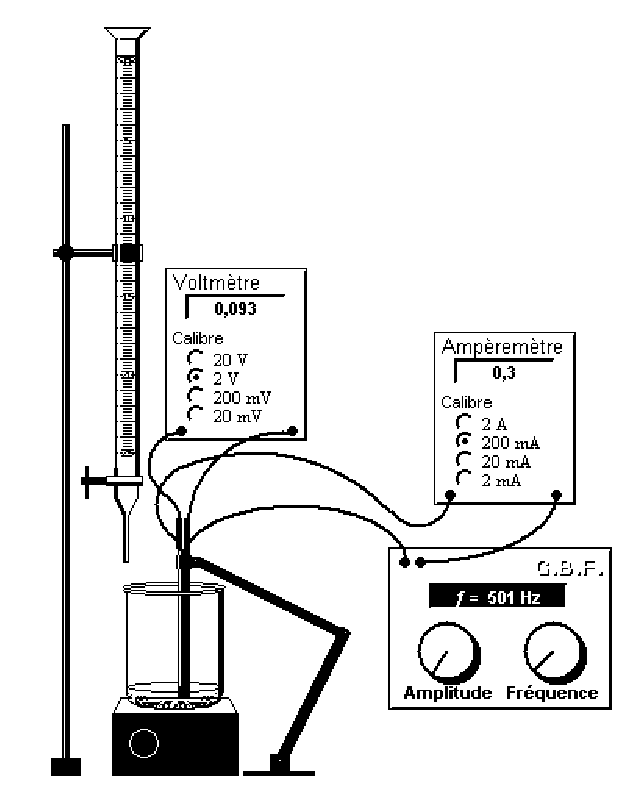
\includegraphics[width=6cm]{tp_prem_s_chimie/tp6_determination_par_conductimetrie_concentration/montage_conductimetrie.png.eps}
\caption{Dispositif exp�rimental}
\end{figure}
\end{center}


\end{multicols}



\subsection{R�sultats}
\begin{enumerate}
\item Calculer la conductance $G$ et compl�ter le tableau suivant.

\begin{arraydata}{6}
\hline
$V_0$ ($mL$)       &  0 &  5 & 10 & 15 & 20 & 25 \\ \hline
\rule[-0.4cm]{0cm}{1cm}
$C$ ($mol.L^{-1}$) &    &    &    &    &    &    \\ \hline
\rule[-0.4cm]{0cm}{1cm}
$G$ ($mS$)         &    &    &    &    &    &    \\ \hline
\end{arraydata}

\item Tracer la courbe d'�talonnage $G = f (C)$.
\end{enumerate}



\pagebreak
%\newpage


\section{D�termination de la concentration en $NaCl$ d'une solution de
  s�rum physiologique}

L'objectif est de d�terminer la concentration du chlorure de sodium dans le s�rum physiologique injectable.

\begin{enumerate}
\item Diluer au $1/100\ieme$ le s�rum physiologique. En pr�parer $500~mL$.

\item D�crire � l'aide de sch�mas le protocole utilis� pour r�aliser
  cette dilution au $1/100\ieme$ et obtenir la solution $S'$.

\item D�terminer la conductance $G'$ de cette solution $S'$.

\item En d�duire la concentration $C'$ du chlorure de sodium dans le
  s�rum physiologique dilu�.

\end{enumerate}


\vressort{3}

\section{Questions compl�mentaires}

%\begin{multicols}{2}

\begin{enumerate}
\item Expliquer comment calculer la concentration $C$ des diff�rentes
  solutions de chlorure de sodium. Donner l'expression de $C$ en
  fonction de $C_0$, $V_0$, $V$.


\item Comment calcule-t-on la conductance $G$ ?

\item Pour quelle raison pratique a-t-on int�r�t � prendre $U =
  1,00~V$ dans les diff�rentes manipulations ?

\item En extrapolant la courbe d'�talonnage, pr�voir la conductance
  d'une portion de solution concentr�e � $T = 58,4~g.L^{-1}$. Mesurer
  la conductance r�elle d'une portion d'une telle solution. Que
  peut-on conclure quant � la m�thode d'�talonnage utilis�e. On donne
  $M_{Na} = 23~g.mol^{-1}$ et $M_{Cl} = 35,5~g.mol^{-1}$.

\item Rappeler la valeur de la concentration $C'$ du chlorure de
  sodium dans le s�rum physiologique dilu�.

\item Comment peut-on alors d�terminer la concentration $C_0'$ du
  chlorure de sodium dans la solution commerciale de s�rum
  physiologique ? Calculer cette concentration $C_0'$ puis le titre
  massique (concentration massique) correspondant $T_0$. Le comparer avec
  les indications figurant sur l'�tiquette du flacon ($0,9~\%$ en masse).
\end{enumerate}


%\vressort{1}
\vressort{3}

\begin{center}
\begin{figure}[H]
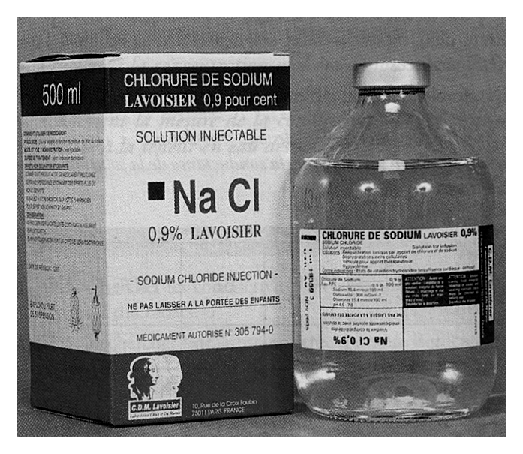
\includegraphics[width=7cm]{tp_prem_s_chimie/tp6_determination_par_conductimetrie_concentration/solution_nacl.png.eps}
\caption{Solution de chlorure de sodium}
\end{figure}
\end{center}


%\end{multicols}


\vressort{3}



\chapitre{Oxydo-r�duction}
\tp{D�termination par conductim�trie\\
de la concentration en solut�\\
d'une solution ionique}


\begin{multicols}{2}

\objectifs{
\item r�aliser une courbe d'�talonnage $G = f(C)$ et en d�duire une
  concentration inconnue.
\item Aborder une limite de la m�thode d'�talonnage.
}
\vspace*{2cm}


\materiel{
\item b�cher $600~mL$
\item fiole jaug�e $500~mL$
\item burette gradu�e $25~mL$
\item pipette jaug�e $5~mL$
\item agitateur magn�tique.
\item solution de chlorure de sodium $S_0$ de concentration $C_0 =
  0,10~mol.L^{-1}$
\item flacon de s�rum physiologique
\item eau d�min�ralis�e
\item g�n�rateur basse fr�quence.
\item 2 multim�tres
\item cellule de conductim�trie.
}


\end{multicols}




\section{R�alisation d'une �chelle de conductance}


\begin{multicols}{2}

\subsection{Protocole op�ratoire}
\begin{enumerate}
\item Rincer la burette, la remplir � l'aide de la solution $S_0$ ajuster le
z�ro.

\item Avec la fiole jaug�e, introduire $V = 500~mL$ d'eau d�min�ralis�e dans
le b�cher.

\item Placer la cellule conductim�trique dans le b�cher et r�aliser le
montage �lectrique correspondant au sch�ma ci-contre. Les 2
multim�tres sont en mode alternatif ($AC$ ou \acsymbol).

\item Sur le GBF, r�gler la fr�quence $500~Hz$ et fixer la tension �
$1,00~V$.

\item Au contenu du b�cher, ajouter les volumes $V_0$ suivants de solution
de chlorure de sodium mesur�s pr�cis�ment gr�ce � la burette. Apr�s
chaque addition, v�rifier que la tension est toujours de $1,00~V$ et
relever la valeur de l'intensit�.

\end{enumerate}




\begin{center}
\begin{figure}[H]
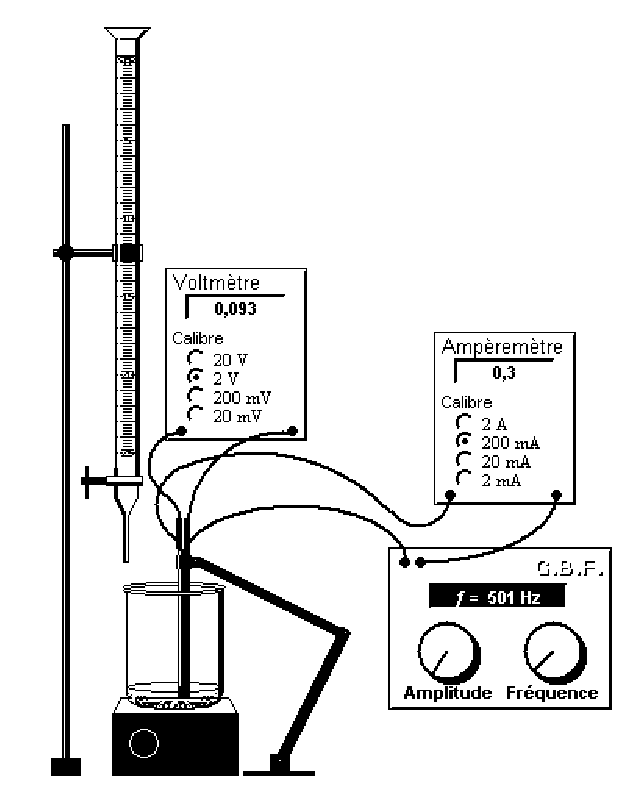
\includegraphics[width=6cm]{tp_prem_s_chimie/tp6_determination_par_conductimetrie_concentration/montage_conductimetrie.png.eps}
\caption{Dispositif exp�rimental}
\end{figure}
\end{center}


\end{multicols}



\subsection{R�sultats}
\begin{enumerate}
\item Calculer la conductance $G$ et compl�ter le tableau suivant.

\begin{arraydata}{6}
\hline
$V_0$ ($mL$)       &  0 &  5 & 10 & 15 & 20 & 25 \\ \hline
\rule[-0.4cm]{0cm}{1cm}
$C$ ($mol.L^{-1}$) &    &    &    &    &    &    \\ \hline
\rule[-0.4cm]{0cm}{1cm}
$G$ ($mS$)         &    &    &    &    &    &    \\ \hline
\end{arraydata}

\item Tracer la courbe d'�talonnage $G = f (C)$.
\end{enumerate}



\pagebreak
%\newpage


\section{D�termination de la concentration en $NaCl$ d'une solution de
  s�rum physiologique}

L'objectif est de d�terminer la concentration du chlorure de sodium dans le s�rum physiologique injectable.

\begin{enumerate}
\item Diluer au $1/100\ieme$ le s�rum physiologique. En pr�parer $500~mL$.

\item D�crire � l'aide de sch�mas le protocole utilis� pour r�aliser
  cette dilution au $1/100\ieme$ et obtenir la solution $S'$.

\item D�terminer la conductance $G'$ de cette solution $S'$.

\item En d�duire la concentration $C'$ du chlorure de sodium dans le
  s�rum physiologique dilu�.

\end{enumerate}


\vressort{3}

\section{Questions compl�mentaires}

%\begin{multicols}{2}

\begin{enumerate}
\item Expliquer comment calculer la concentration $C$ des diff�rentes
  solutions de chlorure de sodium. Donner l'expression de $C$ en
  fonction de $C_0$, $V_0$, $V$.


\item Comment calcule-t-on la conductance $G$ ?

\item Pour quelle raison pratique a-t-on int�r�t � prendre $U =
  1,00~V$ dans les diff�rentes manipulations ?

\item En extrapolant la courbe d'�talonnage, pr�voir la conductance
  d'une portion de solution concentr�e � $T = 58,4~g.L^{-1}$. Mesurer
  la conductance r�elle d'une portion d'une telle solution. Que
  peut-on conclure quant � la m�thode d'�talonnage utilis�e. On donne
  $M_{Na} = 23~g.mol^{-1}$ et $M_{Cl} = 35,5~g.mol^{-1}$.

\item Rappeler la valeur de la concentration $C'$ du chlorure de
  sodium dans le s�rum physiologique dilu�.

\item Comment peut-on alors d�terminer la concentration $C_0'$ du
  chlorure de sodium dans la solution commerciale de s�rum
  physiologique ? Calculer cette concentration $C_0'$ puis le titre
  massique (concentration massique) correspondant $T_0$. Le comparer avec
  les indications figurant sur l'�tiquette du flacon ($0,9~\%$ en masse).
\end{enumerate}


%\vressort{1}
\vressort{3}

\begin{center}
\begin{figure}[H]
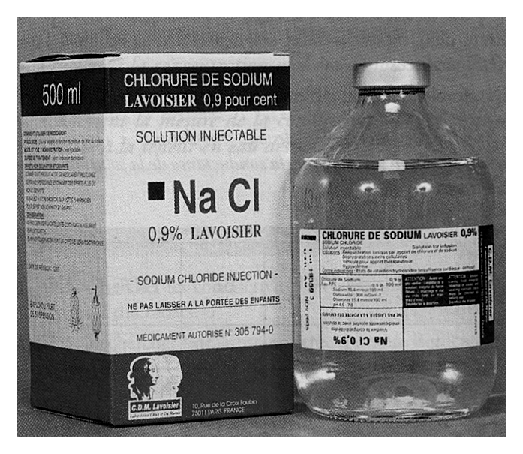
\includegraphics[width=7cm]{tp_prem_s_chimie/tp6_determination_par_conductimetrie_concentration/solution_nacl.png.eps}
\caption{Solution de chlorure de sodium}
\end{figure}
\end{center}


%\end{multicols}


\vressort{3}



\chapitre{Radioactivit�}
\tp{D�termination par conductim�trie\\
de la concentration en solut�\\
d'une solution ionique}


\begin{multicols}{2}

\objectifs{
\item r�aliser une courbe d'�talonnage $G = f(C)$ et en d�duire une
  concentration inconnue.
\item Aborder une limite de la m�thode d'�talonnage.
}
\vspace*{2cm}


\materiel{
\item b�cher $600~mL$
\item fiole jaug�e $500~mL$
\item burette gradu�e $25~mL$
\item pipette jaug�e $5~mL$
\item agitateur magn�tique.
\item solution de chlorure de sodium $S_0$ de concentration $C_0 =
  0,10~mol.L^{-1}$
\item flacon de s�rum physiologique
\item eau d�min�ralis�e
\item g�n�rateur basse fr�quence.
\item 2 multim�tres
\item cellule de conductim�trie.
}


\end{multicols}




\section{R�alisation d'une �chelle de conductance}


\begin{multicols}{2}

\subsection{Protocole op�ratoire}
\begin{enumerate}
\item Rincer la burette, la remplir � l'aide de la solution $S_0$ ajuster le
z�ro.

\item Avec la fiole jaug�e, introduire $V = 500~mL$ d'eau d�min�ralis�e dans
le b�cher.

\item Placer la cellule conductim�trique dans le b�cher et r�aliser le
montage �lectrique correspondant au sch�ma ci-contre. Les 2
multim�tres sont en mode alternatif ($AC$ ou \acsymbol).

\item Sur le GBF, r�gler la fr�quence $500~Hz$ et fixer la tension �
$1,00~V$.

\item Au contenu du b�cher, ajouter les volumes $V_0$ suivants de solution
de chlorure de sodium mesur�s pr�cis�ment gr�ce � la burette. Apr�s
chaque addition, v�rifier que la tension est toujours de $1,00~V$ et
relever la valeur de l'intensit�.

\end{enumerate}




\begin{center}
\begin{figure}[H]
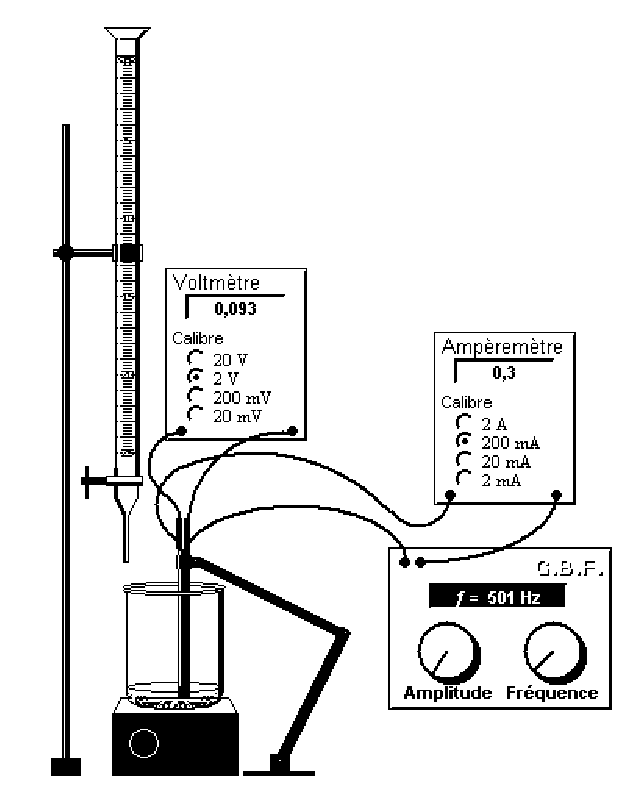
\includegraphics[width=6cm]{tp_prem_s_chimie/tp6_determination_par_conductimetrie_concentration/montage_conductimetrie.png.eps}
\caption{Dispositif exp�rimental}
\end{figure}
\end{center}


\end{multicols}



\subsection{R�sultats}
\begin{enumerate}
\item Calculer la conductance $G$ et compl�ter le tableau suivant.

\begin{arraydata}{6}
\hline
$V_0$ ($mL$)       &  0 &  5 & 10 & 15 & 20 & 25 \\ \hline
\rule[-0.4cm]{0cm}{1cm}
$C$ ($mol.L^{-1}$) &    &    &    &    &    &    \\ \hline
\rule[-0.4cm]{0cm}{1cm}
$G$ ($mS$)         &    &    &    &    &    &    \\ \hline
\end{arraydata}

\item Tracer la courbe d'�talonnage $G = f (C)$.
\end{enumerate}



\pagebreak
%\newpage


\section{D�termination de la concentration en $NaCl$ d'une solution de
  s�rum physiologique}

L'objectif est de d�terminer la concentration du chlorure de sodium dans le s�rum physiologique injectable.

\begin{enumerate}
\item Diluer au $1/100\ieme$ le s�rum physiologique. En pr�parer $500~mL$.

\item D�crire � l'aide de sch�mas le protocole utilis� pour r�aliser
  cette dilution au $1/100\ieme$ et obtenir la solution $S'$.

\item D�terminer la conductance $G'$ de cette solution $S'$.

\item En d�duire la concentration $C'$ du chlorure de sodium dans le
  s�rum physiologique dilu�.

\end{enumerate}


\vressort{3}

\section{Questions compl�mentaires}

%\begin{multicols}{2}

\begin{enumerate}
\item Expliquer comment calculer la concentration $C$ des diff�rentes
  solutions de chlorure de sodium. Donner l'expression de $C$ en
  fonction de $C_0$, $V_0$, $V$.


\item Comment calcule-t-on la conductance $G$ ?

\item Pour quelle raison pratique a-t-on int�r�t � prendre $U =
  1,00~V$ dans les diff�rentes manipulations ?

\item En extrapolant la courbe d'�talonnage, pr�voir la conductance
  d'une portion de solution concentr�e � $T = 58,4~g.L^{-1}$. Mesurer
  la conductance r�elle d'une portion d'une telle solution. Que
  peut-on conclure quant � la m�thode d'�talonnage utilis�e. On donne
  $M_{Na} = 23~g.mol^{-1}$ et $M_{Cl} = 35,5~g.mol^{-1}$.

\item Rappeler la valeur de la concentration $C'$ du chlorure de
  sodium dans le s�rum physiologique dilu�.

\item Comment peut-on alors d�terminer la concentration $C_0'$ du
  chlorure de sodium dans la solution commerciale de s�rum
  physiologique ? Calculer cette concentration $C_0'$ puis le titre
  massique (concentration massique) correspondant $T_0$. Le comparer avec
  les indications figurant sur l'�tiquette du flacon ($0,9~\%$ en masse).
\end{enumerate}


%\vressort{1}
\vressort{3}

\begin{center}
\begin{figure}[H]
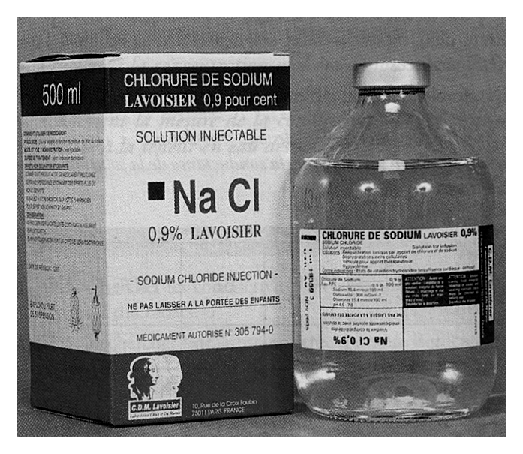
\includegraphics[width=7cm]{tp_prem_s_chimie/tp6_determination_par_conductimetrie_concentration/solution_nacl.png.eps}
\caption{Solution de chlorure de sodium}
\end{figure}
\end{center}


%\end{multicols}


\vressort{3}  % CRAB
% % Jeu avec des d�s : loi de d�croissance radioactive

% R�actions nucl�aires spontan�es

% R�actions nucl�aires provoqu�es


\tp{D�termination par conductim�trie\\
de la concentration en solut�\\
d'une solution ionique}


\begin{multicols}{2}

\objectifs{
\item r�aliser une courbe d'�talonnage $G = f(C)$ et en d�duire une
  concentration inconnue.
\item Aborder une limite de la m�thode d'�talonnage.
}
\vspace*{2cm}


\materiel{
\item b�cher $600~mL$
\item fiole jaug�e $500~mL$
\item burette gradu�e $25~mL$
\item pipette jaug�e $5~mL$
\item agitateur magn�tique.
\item solution de chlorure de sodium $S_0$ de concentration $C_0 =
  0,10~mol.L^{-1}$
\item flacon de s�rum physiologique
\item eau d�min�ralis�e
\item g�n�rateur basse fr�quence.
\item 2 multim�tres
\item cellule de conductim�trie.
}


\end{multicols}




\section{R�alisation d'une �chelle de conductance}


\begin{multicols}{2}

\subsection{Protocole op�ratoire}
\begin{enumerate}
\item Rincer la burette, la remplir � l'aide de la solution $S_0$ ajuster le
z�ro.

\item Avec la fiole jaug�e, introduire $V = 500~mL$ d'eau d�min�ralis�e dans
le b�cher.

\item Placer la cellule conductim�trique dans le b�cher et r�aliser le
montage �lectrique correspondant au sch�ma ci-contre. Les 2
multim�tres sont en mode alternatif ($AC$ ou \acsymbol).

\item Sur le GBF, r�gler la fr�quence $500~Hz$ et fixer la tension �
$1,00~V$.

\item Au contenu du b�cher, ajouter les volumes $V_0$ suivants de solution
de chlorure de sodium mesur�s pr�cis�ment gr�ce � la burette. Apr�s
chaque addition, v�rifier que la tension est toujours de $1,00~V$ et
relever la valeur de l'intensit�.

\end{enumerate}




\begin{center}
\begin{figure}[H]
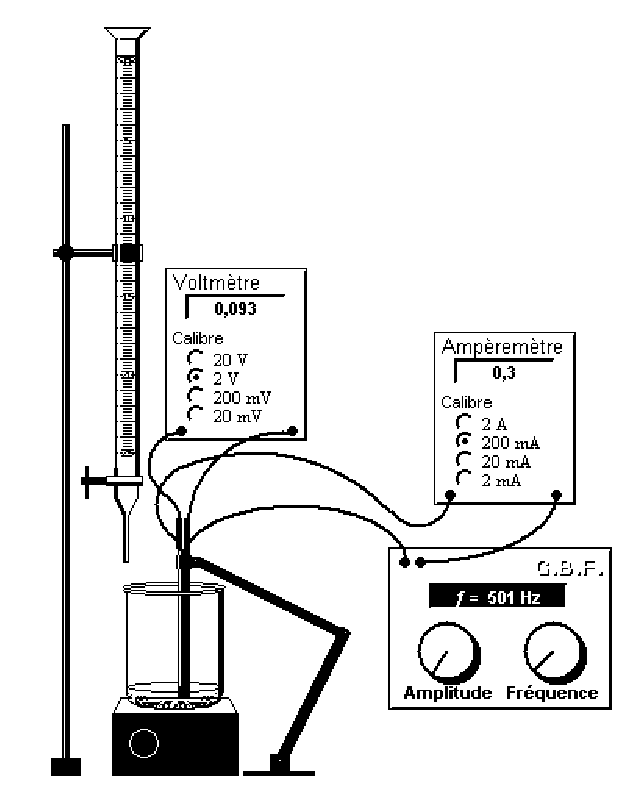
\includegraphics[width=6cm]{tp_prem_s_chimie/tp6_determination_par_conductimetrie_concentration/montage_conductimetrie.png.eps}
\caption{Dispositif exp�rimental}
\end{figure}
\end{center}


\end{multicols}



\subsection{R�sultats}
\begin{enumerate}
\item Calculer la conductance $G$ et compl�ter le tableau suivant.

\begin{arraydata}{6}
\hline
$V_0$ ($mL$)       &  0 &  5 & 10 & 15 & 20 & 25 \\ \hline
\rule[-0.4cm]{0cm}{1cm}
$C$ ($mol.L^{-1}$) &    &    &    &    &    &    \\ \hline
\rule[-0.4cm]{0cm}{1cm}
$G$ ($mS$)         &    &    &    &    &    &    \\ \hline
\end{arraydata}

\item Tracer la courbe d'�talonnage $G = f (C)$.
\end{enumerate}



\pagebreak
%\newpage


\section{D�termination de la concentration en $NaCl$ d'une solution de
  s�rum physiologique}

L'objectif est de d�terminer la concentration du chlorure de sodium dans le s�rum physiologique injectable.

\begin{enumerate}
\item Diluer au $1/100\ieme$ le s�rum physiologique. En pr�parer $500~mL$.

\item D�crire � l'aide de sch�mas le protocole utilis� pour r�aliser
  cette dilution au $1/100\ieme$ et obtenir la solution $S'$.

\item D�terminer la conductance $G'$ de cette solution $S'$.

\item En d�duire la concentration $C'$ du chlorure de sodium dans le
  s�rum physiologique dilu�.

\end{enumerate}


\vressort{3}

\section{Questions compl�mentaires}

%\begin{multicols}{2}

\begin{enumerate}
\item Expliquer comment calculer la concentration $C$ des diff�rentes
  solutions de chlorure de sodium. Donner l'expression de $C$ en
  fonction de $C_0$, $V_0$, $V$.


\item Comment calcule-t-on la conductance $G$ ?

\item Pour quelle raison pratique a-t-on int�r�t � prendre $U =
  1,00~V$ dans les diff�rentes manipulations ?

\item En extrapolant la courbe d'�talonnage, pr�voir la conductance
  d'une portion de solution concentr�e � $T = 58,4~g.L^{-1}$. Mesurer
  la conductance r�elle d'une portion d'une telle solution. Que
  peut-on conclure quant � la m�thode d'�talonnage utilis�e. On donne
  $M_{Na} = 23~g.mol^{-1}$ et $M_{Cl} = 35,5~g.mol^{-1}$.

\item Rappeler la valeur de la concentration $C'$ du chlorure de
  sodium dans le s�rum physiologique dilu�.

\item Comment peut-on alors d�terminer la concentration $C_0'$ du
  chlorure de sodium dans la solution commerciale de s�rum
  physiologique ? Calculer cette concentration $C_0'$ puis le titre
  massique (concentration massique) correspondant $T_0$. Le comparer avec
  les indications figurant sur l'�tiquette du flacon ($0,9~\%$ en masse).
\end{enumerate}


%\vressort{1}
\vressort{3}

\begin{center}
\begin{figure}[H]
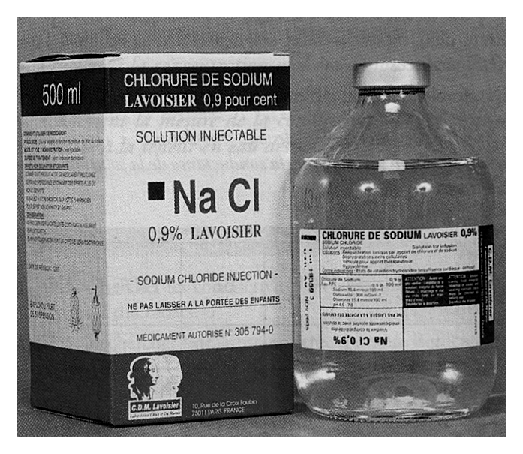
\includegraphics[width=7cm]{tp_prem_s_chimie/tp6_determination_par_conductimetrie_concentration/solution_nacl.png.eps}
\caption{Solution de chlorure de sodium}
\end{figure}
\end{center}


%\end{multicols}


\vressort{3}

\chapitre{La lumi�re}
\tp{D�termination par conductim�trie\\
de la concentration en solut�\\
d'une solution ionique}


\begin{multicols}{2}

\objectifs{
\item r�aliser une courbe d'�talonnage $G = f(C)$ et en d�duire une
  concentration inconnue.
\item Aborder une limite de la m�thode d'�talonnage.
}
\vspace*{2cm}


\materiel{
\item b�cher $600~mL$
\item fiole jaug�e $500~mL$
\item burette gradu�e $25~mL$
\item pipette jaug�e $5~mL$
\item agitateur magn�tique.
\item solution de chlorure de sodium $S_0$ de concentration $C_0 =
  0,10~mol.L^{-1}$
\item flacon de s�rum physiologique
\item eau d�min�ralis�e
\item g�n�rateur basse fr�quence.
\item 2 multim�tres
\item cellule de conductim�trie.
}


\end{multicols}




\section{R�alisation d'une �chelle de conductance}


\begin{multicols}{2}

\subsection{Protocole op�ratoire}
\begin{enumerate}
\item Rincer la burette, la remplir � l'aide de la solution $S_0$ ajuster le
z�ro.

\item Avec la fiole jaug�e, introduire $V = 500~mL$ d'eau d�min�ralis�e dans
le b�cher.

\item Placer la cellule conductim�trique dans le b�cher et r�aliser le
montage �lectrique correspondant au sch�ma ci-contre. Les 2
multim�tres sont en mode alternatif ($AC$ ou \acsymbol).

\item Sur le GBF, r�gler la fr�quence $500~Hz$ et fixer la tension �
$1,00~V$.

\item Au contenu du b�cher, ajouter les volumes $V_0$ suivants de solution
de chlorure de sodium mesur�s pr�cis�ment gr�ce � la burette. Apr�s
chaque addition, v�rifier que la tension est toujours de $1,00~V$ et
relever la valeur de l'intensit�.

\end{enumerate}




\begin{center}
\begin{figure}[H]
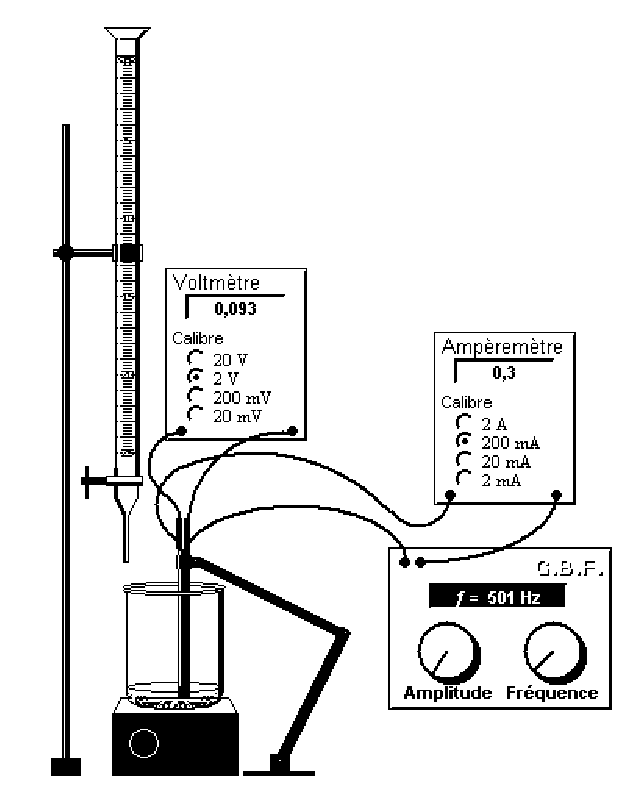
\includegraphics[width=6cm]{tp_prem_s_chimie/tp6_determination_par_conductimetrie_concentration/montage_conductimetrie.png.eps}
\caption{Dispositif exp�rimental}
\end{figure}
\end{center}


\end{multicols}



\subsection{R�sultats}
\begin{enumerate}
\item Calculer la conductance $G$ et compl�ter le tableau suivant.

\begin{arraydata}{6}
\hline
$V_0$ ($mL$)       &  0 &  5 & 10 & 15 & 20 & 25 \\ \hline
\rule[-0.4cm]{0cm}{1cm}
$C$ ($mol.L^{-1}$) &    &    &    &    &    &    \\ \hline
\rule[-0.4cm]{0cm}{1cm}
$G$ ($mS$)         &    &    &    &    &    &    \\ \hline
\end{arraydata}

\item Tracer la courbe d'�talonnage $G = f (C)$.
\end{enumerate}



\pagebreak
%\newpage


\section{D�termination de la concentration en $NaCl$ d'une solution de
  s�rum physiologique}

L'objectif est de d�terminer la concentration du chlorure de sodium dans le s�rum physiologique injectable.

\begin{enumerate}
\item Diluer au $1/100\ieme$ le s�rum physiologique. En pr�parer $500~mL$.

\item D�crire � l'aide de sch�mas le protocole utilis� pour r�aliser
  cette dilution au $1/100\ieme$ et obtenir la solution $S'$.

\item D�terminer la conductance $G'$ de cette solution $S'$.

\item En d�duire la concentration $C'$ du chlorure de sodium dans le
  s�rum physiologique dilu�.

\end{enumerate}


\vressort{3}

\section{Questions compl�mentaires}

%\begin{multicols}{2}

\begin{enumerate}
\item Expliquer comment calculer la concentration $C$ des diff�rentes
  solutions de chlorure de sodium. Donner l'expression de $C$ en
  fonction de $C_0$, $V_0$, $V$.


\item Comment calcule-t-on la conductance $G$ ?

\item Pour quelle raison pratique a-t-on int�r�t � prendre $U =
  1,00~V$ dans les diff�rentes manipulations ?

\item En extrapolant la courbe d'�talonnage, pr�voir la conductance
  d'une portion de solution concentr�e � $T = 58,4~g.L^{-1}$. Mesurer
  la conductance r�elle d'une portion d'une telle solution. Que
  peut-on conclure quant � la m�thode d'�talonnage utilis�e. On donne
  $M_{Na} = 23~g.mol^{-1}$ et $M_{Cl} = 35,5~g.mol^{-1}$.

\item Rappeler la valeur de la concentration $C'$ du chlorure de
  sodium dans le s�rum physiologique dilu�.

\item Comment peut-on alors d�terminer la concentration $C_0'$ du
  chlorure de sodium dans la solution commerciale de s�rum
  physiologique ? Calculer cette concentration $C_0'$ puis le titre
  massique (concentration massique) correspondant $T_0$. Le comparer avec
  les indications figurant sur l'�tiquette du flacon ($0,9~\%$ en masse).
\end{enumerate}


%\vressort{1}
\vressort{3}

\begin{center}
\begin{figure}[H]
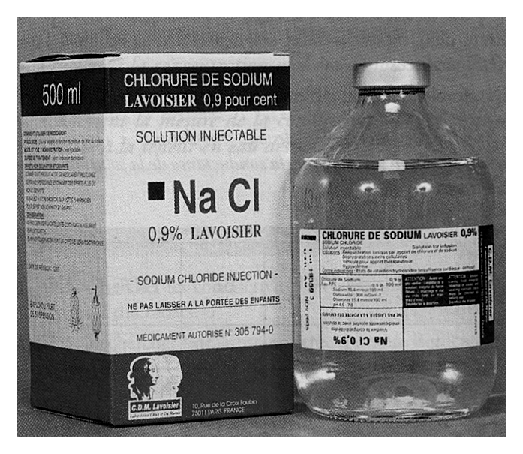
\includegraphics[width=7cm]{tp_prem_s_chimie/tp6_determination_par_conductimetrie_concentration/solution_nacl.png.eps}
\caption{Solution de chlorure de sodium}
\end{figure}
\end{center}


%\end{multicols}


\vressort{3}


% \chapitre{Spectroscopie}
% %\input{
 

% \chapitre{Rayons X}








% \chapitre{Devoir Surveill�} % Term STL B
% \tp{D�termination par conductim�trie\\
de la concentration en solut�\\
d'une solution ionique}


\begin{multicols}{2}

\objectifs{
\item r�aliser une courbe d'�talonnage $G = f(C)$ et en d�duire une
  concentration inconnue.
\item Aborder une limite de la m�thode d'�talonnage.
}
\vspace*{2cm}


\materiel{
\item b�cher $600~mL$
\item fiole jaug�e $500~mL$
\item burette gradu�e $25~mL$
\item pipette jaug�e $5~mL$
\item agitateur magn�tique.
\item solution de chlorure de sodium $S_0$ de concentration $C_0 =
  0,10~mol.L^{-1}$
\item flacon de s�rum physiologique
\item eau d�min�ralis�e
\item g�n�rateur basse fr�quence.
\item 2 multim�tres
\item cellule de conductim�trie.
}


\end{multicols}




\section{R�alisation d'une �chelle de conductance}


\begin{multicols}{2}

\subsection{Protocole op�ratoire}
\begin{enumerate}
\item Rincer la burette, la remplir � l'aide de la solution $S_0$ ajuster le
z�ro.

\item Avec la fiole jaug�e, introduire $V = 500~mL$ d'eau d�min�ralis�e dans
le b�cher.

\item Placer la cellule conductim�trique dans le b�cher et r�aliser le
montage �lectrique correspondant au sch�ma ci-contre. Les 2
multim�tres sont en mode alternatif ($AC$ ou \acsymbol).

\item Sur le GBF, r�gler la fr�quence $500~Hz$ et fixer la tension �
$1,00~V$.

\item Au contenu du b�cher, ajouter les volumes $V_0$ suivants de solution
de chlorure de sodium mesur�s pr�cis�ment gr�ce � la burette. Apr�s
chaque addition, v�rifier que la tension est toujours de $1,00~V$ et
relever la valeur de l'intensit�.

\end{enumerate}




\begin{center}
\begin{figure}[H]
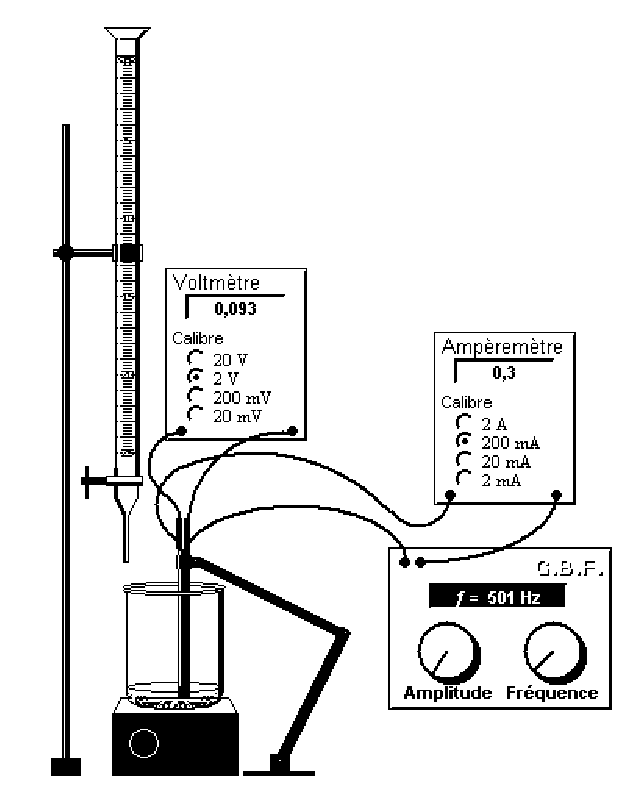
\includegraphics[width=6cm]{tp_prem_s_chimie/tp6_determination_par_conductimetrie_concentration/montage_conductimetrie.png.eps}
\caption{Dispositif exp�rimental}
\end{figure}
\end{center}


\end{multicols}



\subsection{R�sultats}
\begin{enumerate}
\item Calculer la conductance $G$ et compl�ter le tableau suivant.

\begin{arraydata}{6}
\hline
$V_0$ ($mL$)       &  0 &  5 & 10 & 15 & 20 & 25 \\ \hline
\rule[-0.4cm]{0cm}{1cm}
$C$ ($mol.L^{-1}$) &    &    &    &    &    &    \\ \hline
\rule[-0.4cm]{0cm}{1cm}
$G$ ($mS$)         &    &    &    &    &    &    \\ \hline
\end{arraydata}

\item Tracer la courbe d'�talonnage $G = f (C)$.
\end{enumerate}



\pagebreak
%\newpage


\section{D�termination de la concentration en $NaCl$ d'une solution de
  s�rum physiologique}

L'objectif est de d�terminer la concentration du chlorure de sodium dans le s�rum physiologique injectable.

\begin{enumerate}
\item Diluer au $1/100\ieme$ le s�rum physiologique. En pr�parer $500~mL$.

\item D�crire � l'aide de sch�mas le protocole utilis� pour r�aliser
  cette dilution au $1/100\ieme$ et obtenir la solution $S'$.

\item D�terminer la conductance $G'$ de cette solution $S'$.

\item En d�duire la concentration $C'$ du chlorure de sodium dans le
  s�rum physiologique dilu�.

\end{enumerate}


\vressort{3}

\section{Questions compl�mentaires}

%\begin{multicols}{2}

\begin{enumerate}
\item Expliquer comment calculer la concentration $C$ des diff�rentes
  solutions de chlorure de sodium. Donner l'expression de $C$ en
  fonction de $C_0$, $V_0$, $V$.


\item Comment calcule-t-on la conductance $G$ ?

\item Pour quelle raison pratique a-t-on int�r�t � prendre $U =
  1,00~V$ dans les diff�rentes manipulations ?

\item En extrapolant la courbe d'�talonnage, pr�voir la conductance
  d'une portion de solution concentr�e � $T = 58,4~g.L^{-1}$. Mesurer
  la conductance r�elle d'une portion d'une telle solution. Que
  peut-on conclure quant � la m�thode d'�talonnage utilis�e. On donne
  $M_{Na} = 23~g.mol^{-1}$ et $M_{Cl} = 35,5~g.mol^{-1}$.

\item Rappeler la valeur de la concentration $C'$ du chlorure de
  sodium dans le s�rum physiologique dilu�.

\item Comment peut-on alors d�terminer la concentration $C_0'$ du
  chlorure de sodium dans la solution commerciale de s�rum
  physiologique ? Calculer cette concentration $C_0'$ puis le titre
  massique (concentration massique) correspondant $T_0$. Le comparer avec
  les indications figurant sur l'�tiquette du flacon ($0,9~\%$ en masse).
\end{enumerate}


%\vressort{1}
\vressort{3}

\begin{center}
\begin{figure}[H]
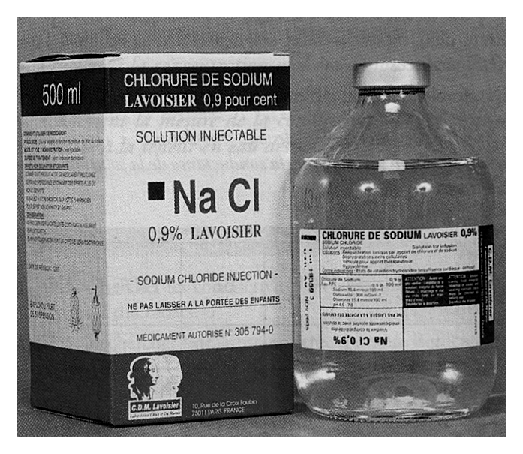
\includegraphics[width=7cm]{tp_prem_s_chimie/tp6_determination_par_conductimetrie_concentration/solution_nacl.png.eps}
\caption{Solution de chlorure de sodium}
\end{figure}
\end{center}


%\end{multicols}


\vressort{3}



\classe{Premi�re\ \\
Sciences et Technologies Industrielles\ \\
G�nie \'Electrotechnique}{Premi�re STI G�nie \'Electrotechnique}





% % tp caract�ristique d'un r�cepteur (moteur � courant continu)

% % potentiel le long d'un circuit �lectrique 
% % tp �tude du montage potentiom�trique (diviseur de tension)

% % tp �tude de la diode PN
% % tp �tude de la diode Zener
% % tp �tude d'un r�gulateur int�gr� de tension 7805



% % tp th�or�me de th�venin / norton
% % tp th�or�me de superposition

\chapitres{Amplificateur Op�rationnel}
\inclure{elec/tp_ao_lin} % tp ao en regime lin�aire
\inclure{elec/tp_ao_lin_eval} % �valutation de tp
 % tp ao en r�gime non lineaire

% tp condensateur (charge � courant constant)


\chapitre{R�gimes variables}
\inclure{elec/tp_elec_oscillo_gbf} % tp regime variable, oscillo, gbf
\inclure{elec/cours_oscillo_gbf}
\inclure{elec/cours_grandeurs_periodiques} % cours grandeurs p�riodiques
\inclure{elec/cours_regimes_transitoires} % cours r�gimes transitoires

% TP RC RL
% TP RLC


% tp transfo, pont de diode, filtrage C, RIT


% tp force �lectromagn�tique (balance �lectromagn�tique ou haut-parleur)

% tp Charge � courant constant d'un condensateur

% tp transistor bipolaire (caract�ristiques)
% tp transistor bipolaire (utilisations)
% tp transistor bipolaire (commutation)

% tp champ magn�tique
% tp r�gime transitoire RC et RL
% tp r�gime transitoire RLC

% tp utilisation du gbf et de l'oscillo
% tp mesure de valeur moyenne et de valeur efficace d'un signal p�riodique




\chapitre{R�gimes sinuso�daux}
\inclure{elec/cours_elec_sin} % cours r�gimes sinuso�daux
\inclure{elec/cours_dipoles_lin_sin} % cours : dip�les lin�aires �l�ementaires en r�gime sinuso�dal

\inclure{elec/cours_asso_serie_dip_sin_reson} % cours : associations de dip�les, r�sonance

% tp : mesure de l'imp�dance et du d�phasage des dipoles �l�mentaires
% association s�rie de dipoles en r�gime sinusoidal
% tp : mesure de d�phasage pour des circuit RC et RL s�rie
% tp : �tude d'un circuit RLC en r�gime sinuso�dal

\inclure{elec/cours_puissance_sin} % cours : puissance en r�gime sinuso�dal monophas�

\inclure{elec/tp_puissance_sin_mono} % tp mesure de puissance en monophas�


% cours : syst�me triphas�s �quilibr�s



% \inclure{elec/tp_redressement_mono_non_comm} % tp redressement mono non command�
% % tp redressement mono command�
% % tp �tude d'une alim continue stabilis�e

% % tp fonctions de l'�lectronique : optocoupleur


% � ajouter si le dernier document contient un nb impair de pages
%\newpage

\classe{Math�matiques Sup�rieures\ \\
PCSI}{Math�matiques Sup�rieures PCSI}

\chapitre{Optique g�om�trique}



% tp_cours_instruments_optique

\inclure{opt/tp_lunette_collimateur} % tp_lunette_collimateur


\inclure{opt/cours_prisme} % cours_prisme


\inclure{opt/tp_prisme_angle} % tp_prisme_angle

\inclure{opt/tp_prisme_indice} % tp_prisme_indice

\inclure{opt/tp_prisme_dispersion} % tp_goniometre








% \chapitre{Optique g�om�trique}
% \tp{D�termination par conductim�trie\\
de la concentration en solut�\\
d'une solution ionique}


\begin{multicols}{2}

\objectifs{
\item r�aliser une courbe d'�talonnage $G = f(C)$ et en d�duire une
  concentration inconnue.
\item Aborder une limite de la m�thode d'�talonnage.
}
\vspace*{2cm}


\materiel{
\item b�cher $600~mL$
\item fiole jaug�e $500~mL$
\item burette gradu�e $25~mL$
\item pipette jaug�e $5~mL$
\item agitateur magn�tique.
\item solution de chlorure de sodium $S_0$ de concentration $C_0 =
  0,10~mol.L^{-1}$
\item flacon de s�rum physiologique
\item eau d�min�ralis�e
\item g�n�rateur basse fr�quence.
\item 2 multim�tres
\item cellule de conductim�trie.
}


\end{multicols}




\section{R�alisation d'une �chelle de conductance}


\begin{multicols}{2}

\subsection{Protocole op�ratoire}
\begin{enumerate}
\item Rincer la burette, la remplir � l'aide de la solution $S_0$ ajuster le
z�ro.

\item Avec la fiole jaug�e, introduire $V = 500~mL$ d'eau d�min�ralis�e dans
le b�cher.

\item Placer la cellule conductim�trique dans le b�cher et r�aliser le
montage �lectrique correspondant au sch�ma ci-contre. Les 2
multim�tres sont en mode alternatif ($AC$ ou \acsymbol).

\item Sur le GBF, r�gler la fr�quence $500~Hz$ et fixer la tension �
$1,00~V$.

\item Au contenu du b�cher, ajouter les volumes $V_0$ suivants de solution
de chlorure de sodium mesur�s pr�cis�ment gr�ce � la burette. Apr�s
chaque addition, v�rifier que la tension est toujours de $1,00~V$ et
relever la valeur de l'intensit�.

\end{enumerate}




\begin{center}
\begin{figure}[H]
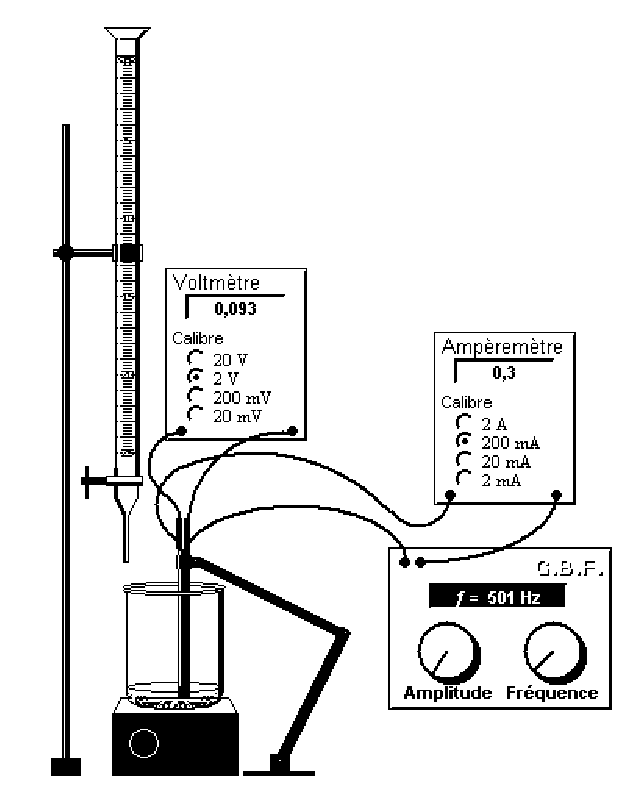
\includegraphics[width=6cm]{tp_prem_s_chimie/tp6_determination_par_conductimetrie_concentration/montage_conductimetrie.png.eps}
\caption{Dispositif exp�rimental}
\end{figure}
\end{center}


\end{multicols}



\subsection{R�sultats}
\begin{enumerate}
\item Calculer la conductance $G$ et compl�ter le tableau suivant.

\begin{arraydata}{6}
\hline
$V_0$ ($mL$)       &  0 &  5 & 10 & 15 & 20 & 25 \\ \hline
\rule[-0.4cm]{0cm}{1cm}
$C$ ($mol.L^{-1}$) &    &    &    &    &    &    \\ \hline
\rule[-0.4cm]{0cm}{1cm}
$G$ ($mS$)         &    &    &    &    &    &    \\ \hline
\end{arraydata}

\item Tracer la courbe d'�talonnage $G = f (C)$.
\end{enumerate}



\pagebreak
%\newpage


\section{D�termination de la concentration en $NaCl$ d'une solution de
  s�rum physiologique}

L'objectif est de d�terminer la concentration du chlorure de sodium dans le s�rum physiologique injectable.

\begin{enumerate}
\item Diluer au $1/100\ieme$ le s�rum physiologique. En pr�parer $500~mL$.

\item D�crire � l'aide de sch�mas le protocole utilis� pour r�aliser
  cette dilution au $1/100\ieme$ et obtenir la solution $S'$.

\item D�terminer la conductance $G'$ de cette solution $S'$.

\item En d�duire la concentration $C'$ du chlorure de sodium dans le
  s�rum physiologique dilu�.

\end{enumerate}


\vressort{3}

\section{Questions compl�mentaires}

%\begin{multicols}{2}

\begin{enumerate}
\item Expliquer comment calculer la concentration $C$ des diff�rentes
  solutions de chlorure de sodium. Donner l'expression de $C$ en
  fonction de $C_0$, $V_0$, $V$.


\item Comment calcule-t-on la conductance $G$ ?

\item Pour quelle raison pratique a-t-on int�r�t � prendre $U =
  1,00~V$ dans les diff�rentes manipulations ?

\item En extrapolant la courbe d'�talonnage, pr�voir la conductance
  d'une portion de solution concentr�e � $T = 58,4~g.L^{-1}$. Mesurer
  la conductance r�elle d'une portion d'une telle solution. Que
  peut-on conclure quant � la m�thode d'�talonnage utilis�e. On donne
  $M_{Na} = 23~g.mol^{-1}$ et $M_{Cl} = 35,5~g.mol^{-1}$.

\item Rappeler la valeur de la concentration $C'$ du chlorure de
  sodium dans le s�rum physiologique dilu�.

\item Comment peut-on alors d�terminer la concentration $C_0'$ du
  chlorure de sodium dans la solution commerciale de s�rum
  physiologique ? Calculer cette concentration $C_0'$ puis le titre
  massique (concentration massique) correspondant $T_0$. Le comparer avec
  les indications figurant sur l'�tiquette du flacon ($0,9~\%$ en masse).
\end{enumerate}


%\vressort{1}
\vressort{3}

\begin{center}
\begin{figure}[H]
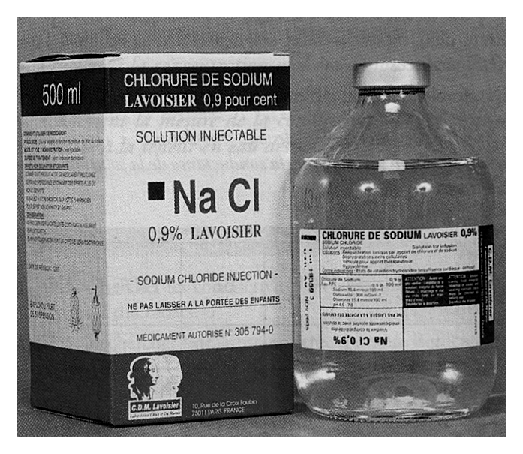
\includegraphics[width=7cm]{tp_prem_s_chimie/tp6_determination_par_conductimetrie_concentration/solution_nacl.png.eps}
\caption{Solution de chlorure de sodium}
\end{figure}
\end{center}


%\end{multicols}


\vressort{3}
%  R�fractom�tre (cf TP Thierry + CDI Chimie)
% Spectroscope (Prisme + goniom�tre)
% Spectrophotom�tre
% Polarim�tre
% Spectre R�sonance Magn�tique Nucl�aire (liaison) http://www.scienceofspectroscopy.info
% TP sup optique ?
% Prisme Mesure d'indice (gonio)
% Prisme Mesure d'angle

%\chapitre{Optique ondulatoire}
% Diffraction (mesure du diam�tre d'un cheveu)
% Interf�rences (Michelson ?)



% TP de MPI (portes logiques, etc..)
% cf A LEQUITTE ENCPB http://www.educnet.education.fr/rnchimie/sommaire.htm


% Document class� par domaines des Sciences Physiques / Physique
% Appliqu�e et non par classe
%% Documents class�s par domaines
% des Sciences Physiques
% Physique Appliqu�e



\chapitre{Electricit�}
\tp{D�termination par conductim�trie\\
de la concentration en solut�\\
d'une solution ionique}


\begin{multicols}{2}

\objectifs{
\item r�aliser une courbe d'�talonnage $G = f(C)$ et en d�duire une
  concentration inconnue.
\item Aborder une limite de la m�thode d'�talonnage.
}
\vspace*{2cm}


\materiel{
\item b�cher $600~mL$
\item fiole jaug�e $500~mL$
\item burette gradu�e $25~mL$
\item pipette jaug�e $5~mL$
\item agitateur magn�tique.
\item solution de chlorure de sodium $S_0$ de concentration $C_0 =
  0,10~mol.L^{-1}$
\item flacon de s�rum physiologique
\item eau d�min�ralis�e
\item g�n�rateur basse fr�quence.
\item 2 multim�tres
\item cellule de conductim�trie.
}


\end{multicols}




\section{R�alisation d'une �chelle de conductance}


\begin{multicols}{2}

\subsection{Protocole op�ratoire}
\begin{enumerate}
\item Rincer la burette, la remplir � l'aide de la solution $S_0$ ajuster le
z�ro.

\item Avec la fiole jaug�e, introduire $V = 500~mL$ d'eau d�min�ralis�e dans
le b�cher.

\item Placer la cellule conductim�trique dans le b�cher et r�aliser le
montage �lectrique correspondant au sch�ma ci-contre. Les 2
multim�tres sont en mode alternatif ($AC$ ou \acsymbol).

\item Sur le GBF, r�gler la fr�quence $500~Hz$ et fixer la tension �
$1,00~V$.

\item Au contenu du b�cher, ajouter les volumes $V_0$ suivants de solution
de chlorure de sodium mesur�s pr�cis�ment gr�ce � la burette. Apr�s
chaque addition, v�rifier que la tension est toujours de $1,00~V$ et
relever la valeur de l'intensit�.

\end{enumerate}




\begin{center}
\begin{figure}[H]
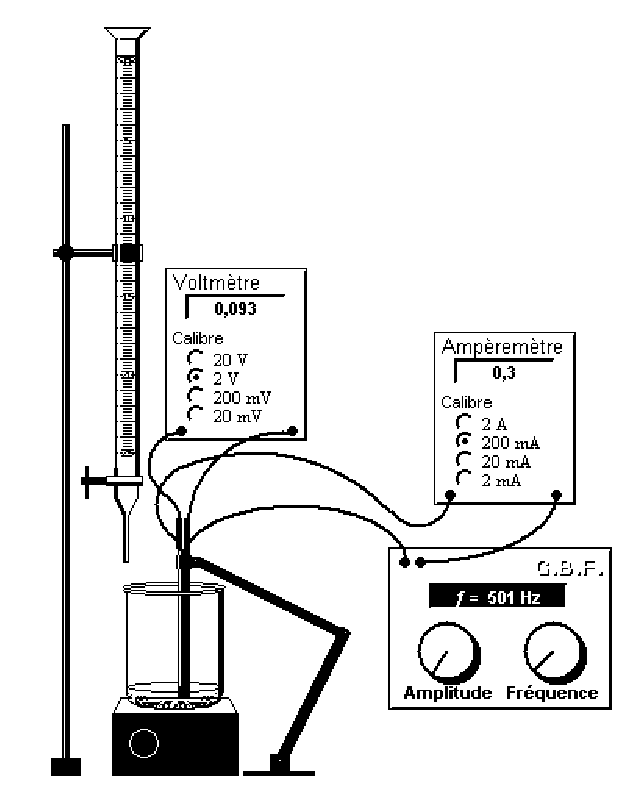
\includegraphics[width=6cm]{tp_prem_s_chimie/tp6_determination_par_conductimetrie_concentration/montage_conductimetrie.png.eps}
\caption{Dispositif exp�rimental}
\end{figure}
\end{center}


\end{multicols}



\subsection{R�sultats}
\begin{enumerate}
\item Calculer la conductance $G$ et compl�ter le tableau suivant.

\begin{arraydata}{6}
\hline
$V_0$ ($mL$)       &  0 &  5 & 10 & 15 & 20 & 25 \\ \hline
\rule[-0.4cm]{0cm}{1cm}
$C$ ($mol.L^{-1}$) &    &    &    &    &    &    \\ \hline
\rule[-0.4cm]{0cm}{1cm}
$G$ ($mS$)         &    &    &    &    &    &    \\ \hline
\end{arraydata}

\item Tracer la courbe d'�talonnage $G = f (C)$.
\end{enumerate}



\pagebreak
%\newpage


\section{D�termination de la concentration en $NaCl$ d'une solution de
  s�rum physiologique}

L'objectif est de d�terminer la concentration du chlorure de sodium dans le s�rum physiologique injectable.

\begin{enumerate}
\item Diluer au $1/100\ieme$ le s�rum physiologique. En pr�parer $500~mL$.

\item D�crire � l'aide de sch�mas le protocole utilis� pour r�aliser
  cette dilution au $1/100\ieme$ et obtenir la solution $S'$.

\item D�terminer la conductance $G'$ de cette solution $S'$.

\item En d�duire la concentration $C'$ du chlorure de sodium dans le
  s�rum physiologique dilu�.

\end{enumerate}


\vressort{3}

\section{Questions compl�mentaires}

%\begin{multicols}{2}

\begin{enumerate}
\item Expliquer comment calculer la concentration $C$ des diff�rentes
  solutions de chlorure de sodium. Donner l'expression de $C$ en
  fonction de $C_0$, $V_0$, $V$.


\item Comment calcule-t-on la conductance $G$ ?

\item Pour quelle raison pratique a-t-on int�r�t � prendre $U =
  1,00~V$ dans les diff�rentes manipulations ?

\item En extrapolant la courbe d'�talonnage, pr�voir la conductance
  d'une portion de solution concentr�e � $T = 58,4~g.L^{-1}$. Mesurer
  la conductance r�elle d'une portion d'une telle solution. Que
  peut-on conclure quant � la m�thode d'�talonnage utilis�e. On donne
  $M_{Na} = 23~g.mol^{-1}$ et $M_{Cl} = 35,5~g.mol^{-1}$.

\item Rappeler la valeur de la concentration $C'$ du chlorure de
  sodium dans le s�rum physiologique dilu�.

\item Comment peut-on alors d�terminer la concentration $C_0'$ du
  chlorure de sodium dans la solution commerciale de s�rum
  physiologique ? Calculer cette concentration $C_0'$ puis le titre
  massique (concentration massique) correspondant $T_0$. Le comparer avec
  les indications figurant sur l'�tiquette du flacon ($0,9~\%$ en masse).
\end{enumerate}


%\vressort{1}
\vressort{3}

\begin{center}
\begin{figure}[H]
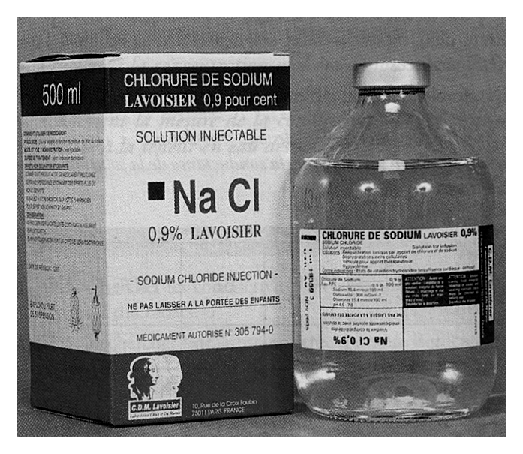
\includegraphics[width=7cm]{tp_prem_s_chimie/tp6_determination_par_conductimetrie_concentration/solution_nacl.png.eps}
\caption{Solution de chlorure de sodium}
\end{figure}
\end{center}


%\end{multicols}


\vressort{3} % cours elec circuit �lectrique

\tp{D�termination par conductim�trie\\
de la concentration en solut�\\
d'une solution ionique}


\begin{multicols}{2}

\objectifs{
\item r�aliser une courbe d'�talonnage $G = f(C)$ et en d�duire une
  concentration inconnue.
\item Aborder une limite de la m�thode d'�talonnage.
}
\vspace*{2cm}


\materiel{
\item b�cher $600~mL$
\item fiole jaug�e $500~mL$
\item burette gradu�e $25~mL$
\item pipette jaug�e $5~mL$
\item agitateur magn�tique.
\item solution de chlorure de sodium $S_0$ de concentration $C_0 =
  0,10~mol.L^{-1}$
\item flacon de s�rum physiologique
\item eau d�min�ralis�e
\item g�n�rateur basse fr�quence.
\item 2 multim�tres
\item cellule de conductim�trie.
}


\end{multicols}




\section{R�alisation d'une �chelle de conductance}


\begin{multicols}{2}

\subsection{Protocole op�ratoire}
\begin{enumerate}
\item Rincer la burette, la remplir � l'aide de la solution $S_0$ ajuster le
z�ro.

\item Avec la fiole jaug�e, introduire $V = 500~mL$ d'eau d�min�ralis�e dans
le b�cher.

\item Placer la cellule conductim�trique dans le b�cher et r�aliser le
montage �lectrique correspondant au sch�ma ci-contre. Les 2
multim�tres sont en mode alternatif ($AC$ ou \acsymbol).

\item Sur le GBF, r�gler la fr�quence $500~Hz$ et fixer la tension �
$1,00~V$.

\item Au contenu du b�cher, ajouter les volumes $V_0$ suivants de solution
de chlorure de sodium mesur�s pr�cis�ment gr�ce � la burette. Apr�s
chaque addition, v�rifier que la tension est toujours de $1,00~V$ et
relever la valeur de l'intensit�.

\end{enumerate}




\begin{center}
\begin{figure}[H]
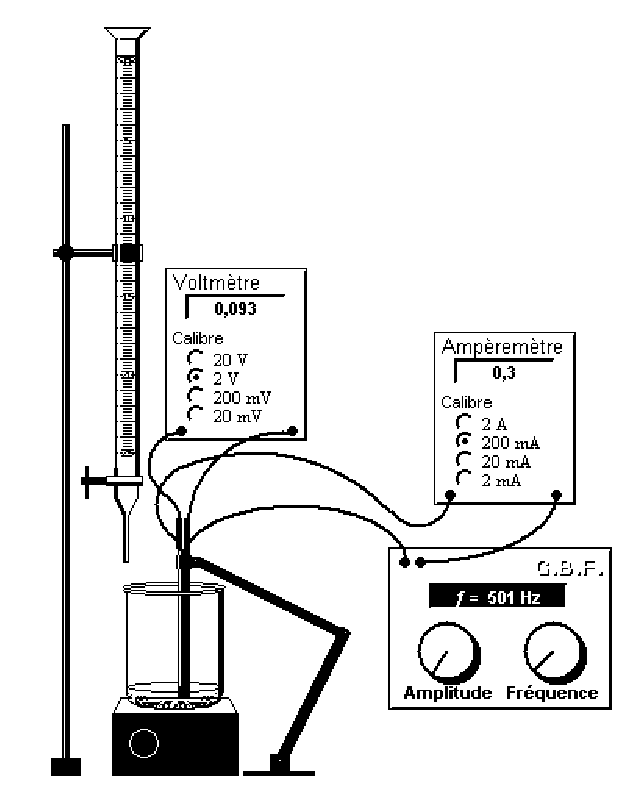
\includegraphics[width=6cm]{tp_prem_s_chimie/tp6_determination_par_conductimetrie_concentration/montage_conductimetrie.png.eps}
\caption{Dispositif exp�rimental}
\end{figure}
\end{center}


\end{multicols}



\subsection{R�sultats}
\begin{enumerate}
\item Calculer la conductance $G$ et compl�ter le tableau suivant.

\begin{arraydata}{6}
\hline
$V_0$ ($mL$)       &  0 &  5 & 10 & 15 & 20 & 25 \\ \hline
\rule[-0.4cm]{0cm}{1cm}
$C$ ($mol.L^{-1}$) &    &    &    &    &    &    \\ \hline
\rule[-0.4cm]{0cm}{1cm}
$G$ ($mS$)         &    &    &    &    &    &    \\ \hline
\end{arraydata}

\item Tracer la courbe d'�talonnage $G = f (C)$.
\end{enumerate}



\pagebreak
%\newpage


\section{D�termination de la concentration en $NaCl$ d'une solution de
  s�rum physiologique}

L'objectif est de d�terminer la concentration du chlorure de sodium dans le s�rum physiologique injectable.

\begin{enumerate}
\item Diluer au $1/100\ieme$ le s�rum physiologique. En pr�parer $500~mL$.

\item D�crire � l'aide de sch�mas le protocole utilis� pour r�aliser
  cette dilution au $1/100\ieme$ et obtenir la solution $S'$.

\item D�terminer la conductance $G'$ de cette solution $S'$.

\item En d�duire la concentration $C'$ du chlorure de sodium dans le
  s�rum physiologique dilu�.

\end{enumerate}


\vressort{3}

\section{Questions compl�mentaires}

%\begin{multicols}{2}

\begin{enumerate}
\item Expliquer comment calculer la concentration $C$ des diff�rentes
  solutions de chlorure de sodium. Donner l'expression de $C$ en
  fonction de $C_0$, $V_0$, $V$.


\item Comment calcule-t-on la conductance $G$ ?

\item Pour quelle raison pratique a-t-on int�r�t � prendre $U =
  1,00~V$ dans les diff�rentes manipulations ?

\item En extrapolant la courbe d'�talonnage, pr�voir la conductance
  d'une portion de solution concentr�e � $T = 58,4~g.L^{-1}$. Mesurer
  la conductance r�elle d'une portion d'une telle solution. Que
  peut-on conclure quant � la m�thode d'�talonnage utilis�e. On donne
  $M_{Na} = 23~g.mol^{-1}$ et $M_{Cl} = 35,5~g.mol^{-1}$.

\item Rappeler la valeur de la concentration $C'$ du chlorure de
  sodium dans le s�rum physiologique dilu�.

\item Comment peut-on alors d�terminer la concentration $C_0'$ du
  chlorure de sodium dans la solution commerciale de s�rum
  physiologique ? Calculer cette concentration $C_0'$ puis le titre
  massique (concentration massique) correspondant $T_0$. Le comparer avec
  les indications figurant sur l'�tiquette du flacon ($0,9~\%$ en masse).
\end{enumerate}


%\vressort{1}
\vressort{3}

\begin{center}
\begin{figure}[H]
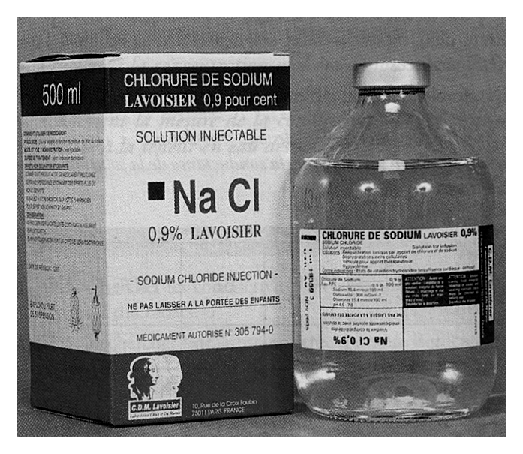
\includegraphics[width=7cm]{tp_prem_s_chimie/tp6_determination_par_conductimetrie_concentration/solution_nacl.png.eps}
\caption{Solution de chlorure de sodium}
\end{figure}
\end{center}


%\end{multicols}


\vressort{3} % tp mesure de tension et d'intensit�

\tp{D�termination par conductim�trie\\
de la concentration en solut�\\
d'une solution ionique}


\begin{multicols}{2}

\objectifs{
\item r�aliser une courbe d'�talonnage $G = f(C)$ et en d�duire une
  concentration inconnue.
\item Aborder une limite de la m�thode d'�talonnage.
}
\vspace*{2cm}


\materiel{
\item b�cher $600~mL$
\item fiole jaug�e $500~mL$
\item burette gradu�e $25~mL$
\item pipette jaug�e $5~mL$
\item agitateur magn�tique.
\item solution de chlorure de sodium $S_0$ de concentration $C_0 =
  0,10~mol.L^{-1}$
\item flacon de s�rum physiologique
\item eau d�min�ralis�e
\item g�n�rateur basse fr�quence.
\item 2 multim�tres
\item cellule de conductim�trie.
}


\end{multicols}




\section{R�alisation d'une �chelle de conductance}


\begin{multicols}{2}

\subsection{Protocole op�ratoire}
\begin{enumerate}
\item Rincer la burette, la remplir � l'aide de la solution $S_0$ ajuster le
z�ro.

\item Avec la fiole jaug�e, introduire $V = 500~mL$ d'eau d�min�ralis�e dans
le b�cher.

\item Placer la cellule conductim�trique dans le b�cher et r�aliser le
montage �lectrique correspondant au sch�ma ci-contre. Les 2
multim�tres sont en mode alternatif ($AC$ ou \acsymbol).

\item Sur le GBF, r�gler la fr�quence $500~Hz$ et fixer la tension �
$1,00~V$.

\item Au contenu du b�cher, ajouter les volumes $V_0$ suivants de solution
de chlorure de sodium mesur�s pr�cis�ment gr�ce � la burette. Apr�s
chaque addition, v�rifier que la tension est toujours de $1,00~V$ et
relever la valeur de l'intensit�.

\end{enumerate}




\begin{center}
\begin{figure}[H]
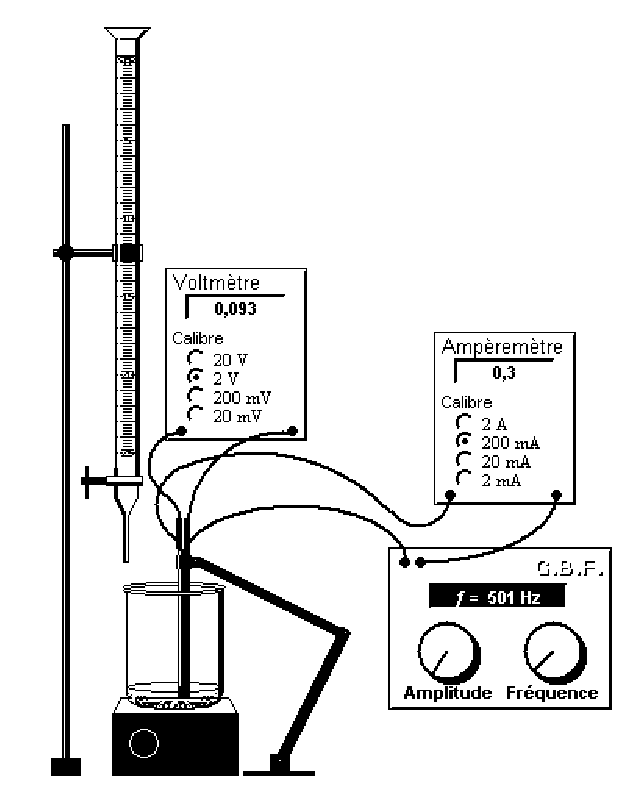
\includegraphics[width=6cm]{tp_prem_s_chimie/tp6_determination_par_conductimetrie_concentration/montage_conductimetrie.png.eps}
\caption{Dispositif exp�rimental}
\end{figure}
\end{center}


\end{multicols}



\subsection{R�sultats}
\begin{enumerate}
\item Calculer la conductance $G$ et compl�ter le tableau suivant.

\begin{arraydata}{6}
\hline
$V_0$ ($mL$)       &  0 &  5 & 10 & 15 & 20 & 25 \\ \hline
\rule[-0.4cm]{0cm}{1cm}
$C$ ($mol.L^{-1}$) &    &    &    &    &    &    \\ \hline
\rule[-0.4cm]{0cm}{1cm}
$G$ ($mS$)         &    &    &    &    &    &    \\ \hline
\end{arraydata}

\item Tracer la courbe d'�talonnage $G = f (C)$.
\end{enumerate}



\pagebreak
%\newpage


\section{D�termination de la concentration en $NaCl$ d'une solution de
  s�rum physiologique}

L'objectif est de d�terminer la concentration du chlorure de sodium dans le s�rum physiologique injectable.

\begin{enumerate}
\item Diluer au $1/100\ieme$ le s�rum physiologique. En pr�parer $500~mL$.

\item D�crire � l'aide de sch�mas le protocole utilis� pour r�aliser
  cette dilution au $1/100\ieme$ et obtenir la solution $S'$.

\item D�terminer la conductance $G'$ de cette solution $S'$.

\item En d�duire la concentration $C'$ du chlorure de sodium dans le
  s�rum physiologique dilu�.

\end{enumerate}


\vressort{3}

\section{Questions compl�mentaires}

%\begin{multicols}{2}

\begin{enumerate}
\item Expliquer comment calculer la concentration $C$ des diff�rentes
  solutions de chlorure de sodium. Donner l'expression de $C$ en
  fonction de $C_0$, $V_0$, $V$.


\item Comment calcule-t-on la conductance $G$ ?

\item Pour quelle raison pratique a-t-on int�r�t � prendre $U =
  1,00~V$ dans les diff�rentes manipulations ?

\item En extrapolant la courbe d'�talonnage, pr�voir la conductance
  d'une portion de solution concentr�e � $T = 58,4~g.L^{-1}$. Mesurer
  la conductance r�elle d'une portion d'une telle solution. Que
  peut-on conclure quant � la m�thode d'�talonnage utilis�e. On donne
  $M_{Na} = 23~g.mol^{-1}$ et $M_{Cl} = 35,5~g.mol^{-1}$.

\item Rappeler la valeur de la concentration $C'$ du chlorure de
  sodium dans le s�rum physiologique dilu�.

\item Comment peut-on alors d�terminer la concentration $C_0'$ du
  chlorure de sodium dans la solution commerciale de s�rum
  physiologique ? Calculer cette concentration $C_0'$ puis le titre
  massique (concentration massique) correspondant $T_0$. Le comparer avec
  les indications figurant sur l'�tiquette du flacon ($0,9~\%$ en masse).
\end{enumerate}


%\vressort{1}
\vressort{3}

\begin{center}
\begin{figure}[H]
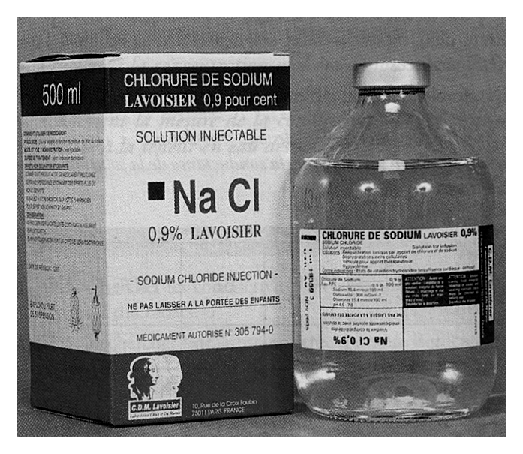
\includegraphics[width=7cm]{tp_prem_s_chimie/tp6_determination_par_conductimetrie_concentration/solution_nacl.png.eps}
\caption{Solution de chlorure de sodium}
\end{figure}
\end{center}


%\end{multicols}


\vressort{3} % document fiche
    % m�thode montage
    % utilisation d'un multim�tre, ...

\tp{D�termination par conductim�trie\\
de la concentration en solut�\\
d'une solution ionique}


\begin{multicols}{2}

\objectifs{
\item r�aliser une courbe d'�talonnage $G = f(C)$ et en d�duire une
  concentration inconnue.
\item Aborder une limite de la m�thode d'�talonnage.
}
\vspace*{2cm}


\materiel{
\item b�cher $600~mL$
\item fiole jaug�e $500~mL$
\item burette gradu�e $25~mL$
\item pipette jaug�e $5~mL$
\item agitateur magn�tique.
\item solution de chlorure de sodium $S_0$ de concentration $C_0 =
  0,10~mol.L^{-1}$
\item flacon de s�rum physiologique
\item eau d�min�ralis�e
\item g�n�rateur basse fr�quence.
\item 2 multim�tres
\item cellule de conductim�trie.
}


\end{multicols}




\section{R�alisation d'une �chelle de conductance}


\begin{multicols}{2}

\subsection{Protocole op�ratoire}
\begin{enumerate}
\item Rincer la burette, la remplir � l'aide de la solution $S_0$ ajuster le
z�ro.

\item Avec la fiole jaug�e, introduire $V = 500~mL$ d'eau d�min�ralis�e dans
le b�cher.

\item Placer la cellule conductim�trique dans le b�cher et r�aliser le
montage �lectrique correspondant au sch�ma ci-contre. Les 2
multim�tres sont en mode alternatif ($AC$ ou \acsymbol).

\item Sur le GBF, r�gler la fr�quence $500~Hz$ et fixer la tension �
$1,00~V$.

\item Au contenu du b�cher, ajouter les volumes $V_0$ suivants de solution
de chlorure de sodium mesur�s pr�cis�ment gr�ce � la burette. Apr�s
chaque addition, v�rifier que la tension est toujours de $1,00~V$ et
relever la valeur de l'intensit�.

\end{enumerate}




\begin{center}
\begin{figure}[H]
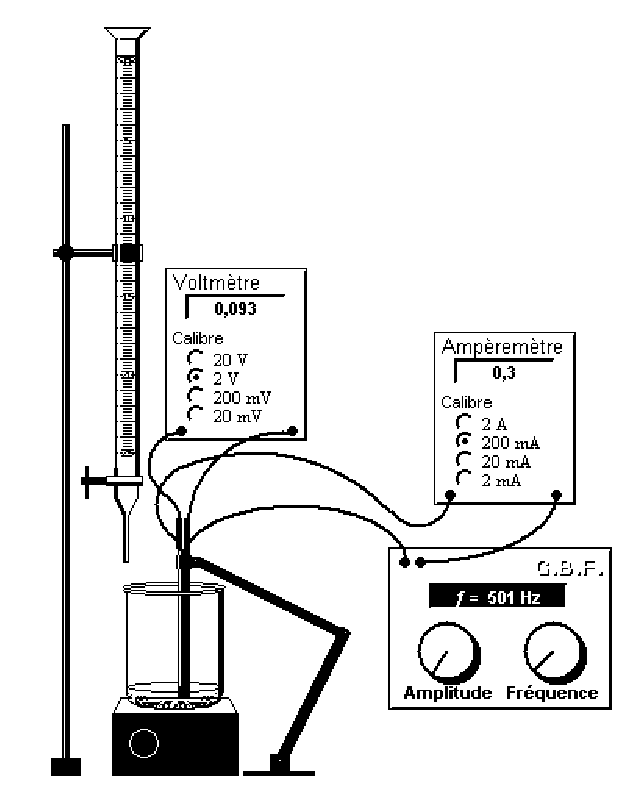
\includegraphics[width=6cm]{tp_prem_s_chimie/tp6_determination_par_conductimetrie_concentration/montage_conductimetrie.png.eps}
\caption{Dispositif exp�rimental}
\end{figure}
\end{center}


\end{multicols}



\subsection{R�sultats}
\begin{enumerate}
\item Calculer la conductance $G$ et compl�ter le tableau suivant.

\begin{arraydata}{6}
\hline
$V_0$ ($mL$)       &  0 &  5 & 10 & 15 & 20 & 25 \\ \hline
\rule[-0.4cm]{0cm}{1cm}
$C$ ($mol.L^{-1}$) &    &    &    &    &    &    \\ \hline
\rule[-0.4cm]{0cm}{1cm}
$G$ ($mS$)         &    &    &    &    &    &    \\ \hline
\end{arraydata}

\item Tracer la courbe d'�talonnage $G = f (C)$.
\end{enumerate}



\pagebreak
%\newpage


\section{D�termination de la concentration en $NaCl$ d'une solution de
  s�rum physiologique}

L'objectif est de d�terminer la concentration du chlorure de sodium dans le s�rum physiologique injectable.

\begin{enumerate}
\item Diluer au $1/100\ieme$ le s�rum physiologique. En pr�parer $500~mL$.

\item D�crire � l'aide de sch�mas le protocole utilis� pour r�aliser
  cette dilution au $1/100\ieme$ et obtenir la solution $S'$.

\item D�terminer la conductance $G'$ de cette solution $S'$.

\item En d�duire la concentration $C'$ du chlorure de sodium dans le
  s�rum physiologique dilu�.

\end{enumerate}


\vressort{3}

\section{Questions compl�mentaires}

%\begin{multicols}{2}

\begin{enumerate}
\item Expliquer comment calculer la concentration $C$ des diff�rentes
  solutions de chlorure de sodium. Donner l'expression de $C$ en
  fonction de $C_0$, $V_0$, $V$.


\item Comment calcule-t-on la conductance $G$ ?

\item Pour quelle raison pratique a-t-on int�r�t � prendre $U =
  1,00~V$ dans les diff�rentes manipulations ?

\item En extrapolant la courbe d'�talonnage, pr�voir la conductance
  d'une portion de solution concentr�e � $T = 58,4~g.L^{-1}$. Mesurer
  la conductance r�elle d'une portion d'une telle solution. Que
  peut-on conclure quant � la m�thode d'�talonnage utilis�e. On donne
  $M_{Na} = 23~g.mol^{-1}$ et $M_{Cl} = 35,5~g.mol^{-1}$.

\item Rappeler la valeur de la concentration $C'$ du chlorure de
  sodium dans le s�rum physiologique dilu�.

\item Comment peut-on alors d�terminer la concentration $C_0'$ du
  chlorure de sodium dans la solution commerciale de s�rum
  physiologique ? Calculer cette concentration $C_0'$ puis le titre
  massique (concentration massique) correspondant $T_0$. Le comparer avec
  les indications figurant sur l'�tiquette du flacon ($0,9~\%$ en masse).
\end{enumerate}


%\vressort{1}
\vressort{3}

\begin{center}
\begin{figure}[H]
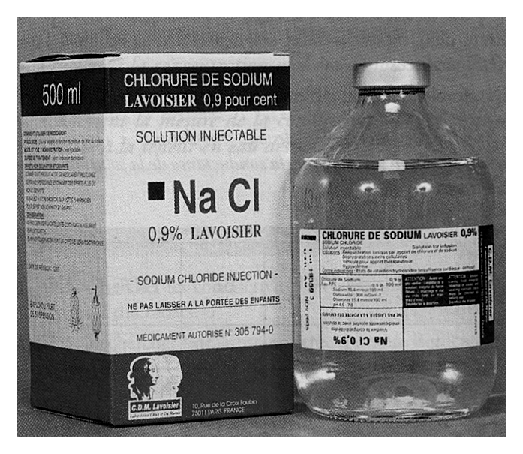
\includegraphics[width=7cm]{tp_prem_s_chimie/tp6_determination_par_conductimetrie_concentration/solution_nacl.png.eps}
\caption{Solution de chlorure de sodium}
\end{figure}
\end{center}


%\end{multicols}


\vressort{3} % tp loi d'ohm

\tp{D�termination par conductim�trie\\
de la concentration en solut�\\
d'une solution ionique}


\begin{multicols}{2}

\objectifs{
\item r�aliser une courbe d'�talonnage $G = f(C)$ et en d�duire une
  concentration inconnue.
\item Aborder une limite de la m�thode d'�talonnage.
}
\vspace*{2cm}


\materiel{
\item b�cher $600~mL$
\item fiole jaug�e $500~mL$
\item burette gradu�e $25~mL$
\item pipette jaug�e $5~mL$
\item agitateur magn�tique.
\item solution de chlorure de sodium $S_0$ de concentration $C_0 =
  0,10~mol.L^{-1}$
\item flacon de s�rum physiologique
\item eau d�min�ralis�e
\item g�n�rateur basse fr�quence.
\item 2 multim�tres
\item cellule de conductim�trie.
}


\end{multicols}




\section{R�alisation d'une �chelle de conductance}


\begin{multicols}{2}

\subsection{Protocole op�ratoire}
\begin{enumerate}
\item Rincer la burette, la remplir � l'aide de la solution $S_0$ ajuster le
z�ro.

\item Avec la fiole jaug�e, introduire $V = 500~mL$ d'eau d�min�ralis�e dans
le b�cher.

\item Placer la cellule conductim�trique dans le b�cher et r�aliser le
montage �lectrique correspondant au sch�ma ci-contre. Les 2
multim�tres sont en mode alternatif ($AC$ ou \acsymbol).

\item Sur le GBF, r�gler la fr�quence $500~Hz$ et fixer la tension �
$1,00~V$.

\item Au contenu du b�cher, ajouter les volumes $V_0$ suivants de solution
de chlorure de sodium mesur�s pr�cis�ment gr�ce � la burette. Apr�s
chaque addition, v�rifier que la tension est toujours de $1,00~V$ et
relever la valeur de l'intensit�.

\end{enumerate}




\begin{center}
\begin{figure}[H]
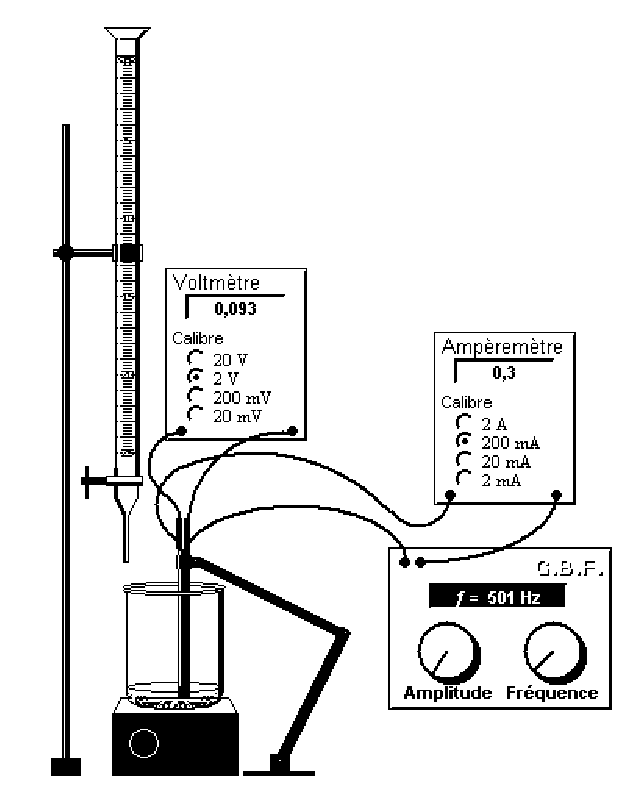
\includegraphics[width=6cm]{tp_prem_s_chimie/tp6_determination_par_conductimetrie_concentration/montage_conductimetrie.png.eps}
\caption{Dispositif exp�rimental}
\end{figure}
\end{center}


\end{multicols}



\subsection{R�sultats}
\begin{enumerate}
\item Calculer la conductance $G$ et compl�ter le tableau suivant.

\begin{arraydata}{6}
\hline
$V_0$ ($mL$)       &  0 &  5 & 10 & 15 & 20 & 25 \\ \hline
\rule[-0.4cm]{0cm}{1cm}
$C$ ($mol.L^{-1}$) &    &    &    &    &    &    \\ \hline
\rule[-0.4cm]{0cm}{1cm}
$G$ ($mS$)         &    &    &    &    &    &    \\ \hline
\end{arraydata}

\item Tracer la courbe d'�talonnage $G = f (C)$.
\end{enumerate}



\pagebreak
%\newpage


\section{D�termination de la concentration en $NaCl$ d'une solution de
  s�rum physiologique}

L'objectif est de d�terminer la concentration du chlorure de sodium dans le s�rum physiologique injectable.

\begin{enumerate}
\item Diluer au $1/100\ieme$ le s�rum physiologique. En pr�parer $500~mL$.

\item D�crire � l'aide de sch�mas le protocole utilis� pour r�aliser
  cette dilution au $1/100\ieme$ et obtenir la solution $S'$.

\item D�terminer la conductance $G'$ de cette solution $S'$.

\item En d�duire la concentration $C'$ du chlorure de sodium dans le
  s�rum physiologique dilu�.

\end{enumerate}


\vressort{3}

\section{Questions compl�mentaires}

%\begin{multicols}{2}

\begin{enumerate}
\item Expliquer comment calculer la concentration $C$ des diff�rentes
  solutions de chlorure de sodium. Donner l'expression de $C$ en
  fonction de $C_0$, $V_0$, $V$.


\item Comment calcule-t-on la conductance $G$ ?

\item Pour quelle raison pratique a-t-on int�r�t � prendre $U =
  1,00~V$ dans les diff�rentes manipulations ?

\item En extrapolant la courbe d'�talonnage, pr�voir la conductance
  d'une portion de solution concentr�e � $T = 58,4~g.L^{-1}$. Mesurer
  la conductance r�elle d'une portion d'une telle solution. Que
  peut-on conclure quant � la m�thode d'�talonnage utilis�e. On donne
  $M_{Na} = 23~g.mol^{-1}$ et $M_{Cl} = 35,5~g.mol^{-1}$.

\item Rappeler la valeur de la concentration $C'$ du chlorure de
  sodium dans le s�rum physiologique dilu�.

\item Comment peut-on alors d�terminer la concentration $C_0'$ du
  chlorure de sodium dans la solution commerciale de s�rum
  physiologique ? Calculer cette concentration $C_0'$ puis le titre
  massique (concentration massique) correspondant $T_0$. Le comparer avec
  les indications figurant sur l'�tiquette du flacon ($0,9~\%$ en masse).
\end{enumerate}


%\vressort{1}
\vressort{3}

\begin{center}
\begin{figure}[H]
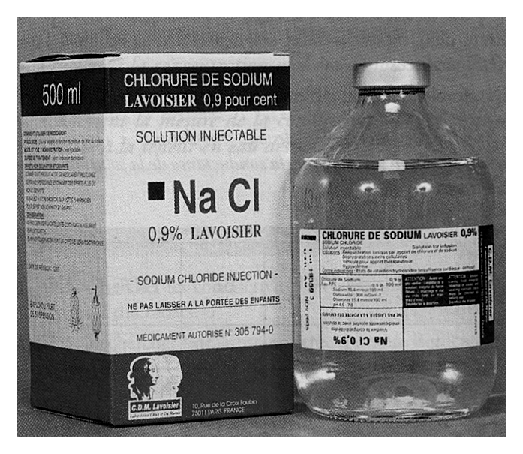
\includegraphics[width=7cm]{tp_prem_s_chimie/tp6_determination_par_conductimetrie_concentration/solution_nacl.png.eps}
\caption{Solution de chlorure de sodium}
\end{figure}
\end{center}


%\end{multicols}


\vressort{3} % tp associations de R

% association r s�rie (trac� U en fonction de I et montrer qu'on ajoute U)
% association r parall�le (trac� U en fonction de I et montrer qu'on ajoute I)

\tp{D�termination par conductim�trie\\
de la concentration en solut�\\
d'une solution ionique}


\begin{multicols}{2}

\objectifs{
\item r�aliser une courbe d'�talonnage $G = f(C)$ et en d�duire une
  concentration inconnue.
\item Aborder une limite de la m�thode d'�talonnage.
}
\vspace*{2cm}


\materiel{
\item b�cher $600~mL$
\item fiole jaug�e $500~mL$
\item burette gradu�e $25~mL$
\item pipette jaug�e $5~mL$
\item agitateur magn�tique.
\item solution de chlorure de sodium $S_0$ de concentration $C_0 =
  0,10~mol.L^{-1}$
\item flacon de s�rum physiologique
\item eau d�min�ralis�e
\item g�n�rateur basse fr�quence.
\item 2 multim�tres
\item cellule de conductim�trie.
}


\end{multicols}




\section{R�alisation d'une �chelle de conductance}


\begin{multicols}{2}

\subsection{Protocole op�ratoire}
\begin{enumerate}
\item Rincer la burette, la remplir � l'aide de la solution $S_0$ ajuster le
z�ro.

\item Avec la fiole jaug�e, introduire $V = 500~mL$ d'eau d�min�ralis�e dans
le b�cher.

\item Placer la cellule conductim�trique dans le b�cher et r�aliser le
montage �lectrique correspondant au sch�ma ci-contre. Les 2
multim�tres sont en mode alternatif ($AC$ ou \acsymbol).

\item Sur le GBF, r�gler la fr�quence $500~Hz$ et fixer la tension �
$1,00~V$.

\item Au contenu du b�cher, ajouter les volumes $V_0$ suivants de solution
de chlorure de sodium mesur�s pr�cis�ment gr�ce � la burette. Apr�s
chaque addition, v�rifier que la tension est toujours de $1,00~V$ et
relever la valeur de l'intensit�.

\end{enumerate}




\begin{center}
\begin{figure}[H]
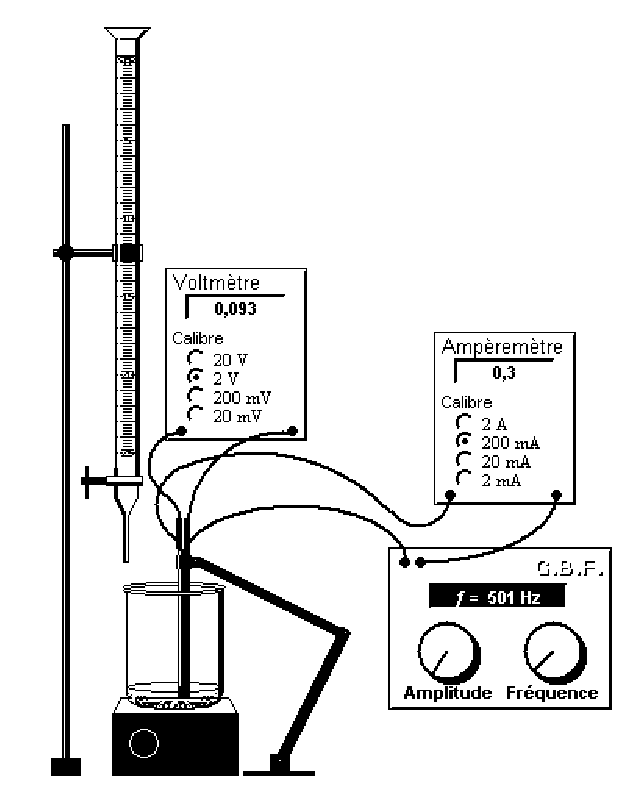
\includegraphics[width=6cm]{tp_prem_s_chimie/tp6_determination_par_conductimetrie_concentration/montage_conductimetrie.png.eps}
\caption{Dispositif exp�rimental}
\end{figure}
\end{center}


\end{multicols}



\subsection{R�sultats}
\begin{enumerate}
\item Calculer la conductance $G$ et compl�ter le tableau suivant.

\begin{arraydata}{6}
\hline
$V_0$ ($mL$)       &  0 &  5 & 10 & 15 & 20 & 25 \\ \hline
\rule[-0.4cm]{0cm}{1cm}
$C$ ($mol.L^{-1}$) &    &    &    &    &    &    \\ \hline
\rule[-0.4cm]{0cm}{1cm}
$G$ ($mS$)         &    &    &    &    &    &    \\ \hline
\end{arraydata}

\item Tracer la courbe d'�talonnage $G = f (C)$.
\end{enumerate}



\pagebreak
%\newpage


\section{D�termination de la concentration en $NaCl$ d'une solution de
  s�rum physiologique}

L'objectif est de d�terminer la concentration du chlorure de sodium dans le s�rum physiologique injectable.

\begin{enumerate}
\item Diluer au $1/100\ieme$ le s�rum physiologique. En pr�parer $500~mL$.

\item D�crire � l'aide de sch�mas le protocole utilis� pour r�aliser
  cette dilution au $1/100\ieme$ et obtenir la solution $S'$.

\item D�terminer la conductance $G'$ de cette solution $S'$.

\item En d�duire la concentration $C'$ du chlorure de sodium dans le
  s�rum physiologique dilu�.

\end{enumerate}


\vressort{3}

\section{Questions compl�mentaires}

%\begin{multicols}{2}

\begin{enumerate}
\item Expliquer comment calculer la concentration $C$ des diff�rentes
  solutions de chlorure de sodium. Donner l'expression de $C$ en
  fonction de $C_0$, $V_0$, $V$.


\item Comment calcule-t-on la conductance $G$ ?

\item Pour quelle raison pratique a-t-on int�r�t � prendre $U =
  1,00~V$ dans les diff�rentes manipulations ?

\item En extrapolant la courbe d'�talonnage, pr�voir la conductance
  d'une portion de solution concentr�e � $T = 58,4~g.L^{-1}$. Mesurer
  la conductance r�elle d'une portion d'une telle solution. Que
  peut-on conclure quant � la m�thode d'�talonnage utilis�e. On donne
  $M_{Na} = 23~g.mol^{-1}$ et $M_{Cl} = 35,5~g.mol^{-1}$.

\item Rappeler la valeur de la concentration $C'$ du chlorure de
  sodium dans le s�rum physiologique dilu�.

\item Comment peut-on alors d�terminer la concentration $C_0'$ du
  chlorure de sodium dans la solution commerciale de s�rum
  physiologique ? Calculer cette concentration $C_0'$ puis le titre
  massique (concentration massique) correspondant $T_0$. Le comparer avec
  les indications figurant sur l'�tiquette du flacon ($0,9~\%$ en masse).
\end{enumerate}


%\vressort{1}
\vressort{3}

\begin{center}
\begin{figure}[H]
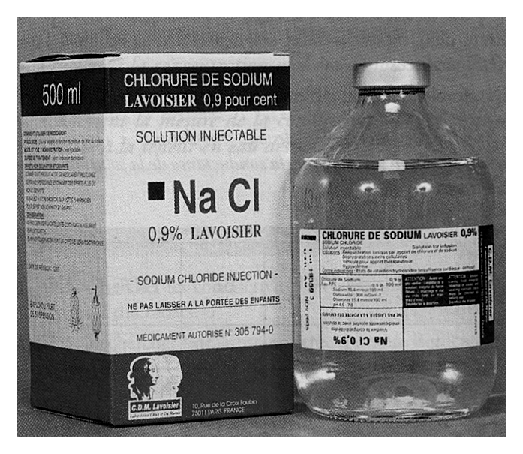
\includegraphics[width=7cm]{tp_prem_s_chimie/tp6_determination_par_conductimetrie_concentration/solution_nacl.png.eps}
\caption{Solution de chlorure de sodium}
\end{figure}
\end{center}


%\end{multicols}


\vressort{3} % cours elec g�n�rateurs, r�cepteurs

\tp{D�termination par conductim�trie\\
de la concentration en solut�\\
d'une solution ionique}


\begin{multicols}{2}

\objectifs{
\item r�aliser une courbe d'�talonnage $G = f(C)$ et en d�duire une
  concentration inconnue.
\item Aborder une limite de la m�thode d'�talonnage.
}
\vspace*{2cm}


\materiel{
\item b�cher $600~mL$
\item fiole jaug�e $500~mL$
\item burette gradu�e $25~mL$
\item pipette jaug�e $5~mL$
\item agitateur magn�tique.
\item solution de chlorure de sodium $S_0$ de concentration $C_0 =
  0,10~mol.L^{-1}$
\item flacon de s�rum physiologique
\item eau d�min�ralis�e
\item g�n�rateur basse fr�quence.
\item 2 multim�tres
\item cellule de conductim�trie.
}


\end{multicols}




\section{R�alisation d'une �chelle de conductance}


\begin{multicols}{2}

\subsection{Protocole op�ratoire}
\begin{enumerate}
\item Rincer la burette, la remplir � l'aide de la solution $S_0$ ajuster le
z�ro.

\item Avec la fiole jaug�e, introduire $V = 500~mL$ d'eau d�min�ralis�e dans
le b�cher.

\item Placer la cellule conductim�trique dans le b�cher et r�aliser le
montage �lectrique correspondant au sch�ma ci-contre. Les 2
multim�tres sont en mode alternatif ($AC$ ou \acsymbol).

\item Sur le GBF, r�gler la fr�quence $500~Hz$ et fixer la tension �
$1,00~V$.

\item Au contenu du b�cher, ajouter les volumes $V_0$ suivants de solution
de chlorure de sodium mesur�s pr�cis�ment gr�ce � la burette. Apr�s
chaque addition, v�rifier que la tension est toujours de $1,00~V$ et
relever la valeur de l'intensit�.

\end{enumerate}




\begin{center}
\begin{figure}[H]
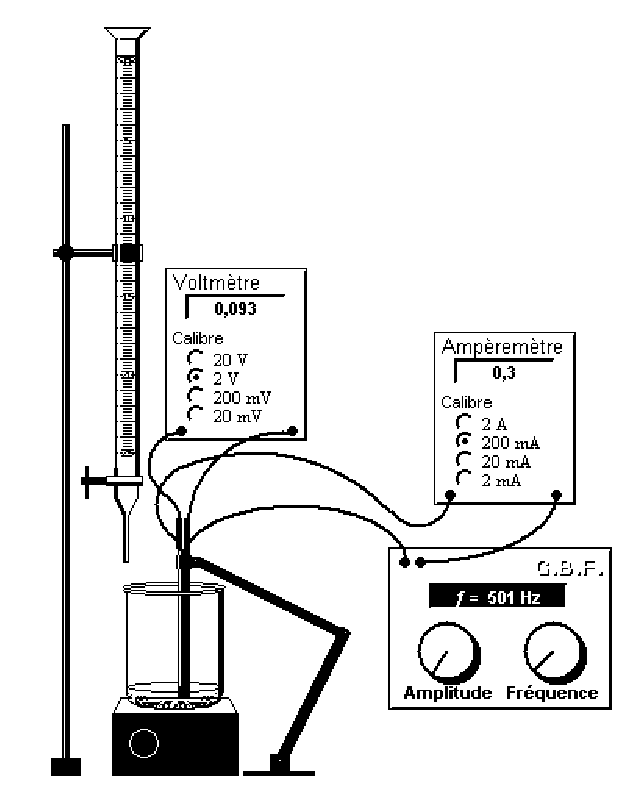
\includegraphics[width=6cm]{tp_prem_s_chimie/tp6_determination_par_conductimetrie_concentration/montage_conductimetrie.png.eps}
\caption{Dispositif exp�rimental}
\end{figure}
\end{center}


\end{multicols}



\subsection{R�sultats}
\begin{enumerate}
\item Calculer la conductance $G$ et compl�ter le tableau suivant.

\begin{arraydata}{6}
\hline
$V_0$ ($mL$)       &  0 &  5 & 10 & 15 & 20 & 25 \\ \hline
\rule[-0.4cm]{0cm}{1cm}
$C$ ($mol.L^{-1}$) &    &    &    &    &    &    \\ \hline
\rule[-0.4cm]{0cm}{1cm}
$G$ ($mS$)         &    &    &    &    &    &    \\ \hline
\end{arraydata}

\item Tracer la courbe d'�talonnage $G = f (C)$.
\end{enumerate}



\pagebreak
%\newpage


\section{D�termination de la concentration en $NaCl$ d'une solution de
  s�rum physiologique}

L'objectif est de d�terminer la concentration du chlorure de sodium dans le s�rum physiologique injectable.

\begin{enumerate}
\item Diluer au $1/100\ieme$ le s�rum physiologique. En pr�parer $500~mL$.

\item D�crire � l'aide de sch�mas le protocole utilis� pour r�aliser
  cette dilution au $1/100\ieme$ et obtenir la solution $S'$.

\item D�terminer la conductance $G'$ de cette solution $S'$.

\item En d�duire la concentration $C'$ du chlorure de sodium dans le
  s�rum physiologique dilu�.

\end{enumerate}


\vressort{3}

\section{Questions compl�mentaires}

%\begin{multicols}{2}

\begin{enumerate}
\item Expliquer comment calculer la concentration $C$ des diff�rentes
  solutions de chlorure de sodium. Donner l'expression de $C$ en
  fonction de $C_0$, $V_0$, $V$.


\item Comment calcule-t-on la conductance $G$ ?

\item Pour quelle raison pratique a-t-on int�r�t � prendre $U =
  1,00~V$ dans les diff�rentes manipulations ?

\item En extrapolant la courbe d'�talonnage, pr�voir la conductance
  d'une portion de solution concentr�e � $T = 58,4~g.L^{-1}$. Mesurer
  la conductance r�elle d'une portion d'une telle solution. Que
  peut-on conclure quant � la m�thode d'�talonnage utilis�e. On donne
  $M_{Na} = 23~g.mol^{-1}$ et $M_{Cl} = 35,5~g.mol^{-1}$.

\item Rappeler la valeur de la concentration $C'$ du chlorure de
  sodium dans le s�rum physiologique dilu�.

\item Comment peut-on alors d�terminer la concentration $C_0'$ du
  chlorure de sodium dans la solution commerciale de s�rum
  physiologique ? Calculer cette concentration $C_0'$ puis le titre
  massique (concentration massique) correspondant $T_0$. Le comparer avec
  les indications figurant sur l'�tiquette du flacon ($0,9~\%$ en masse).
\end{enumerate}


%\vressort{1}
\vressort{3}

\begin{center}
\begin{figure}[H]
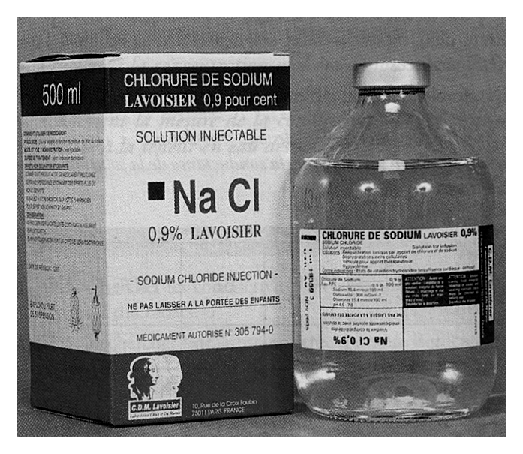
\includegraphics[width=7cm]{tp_prem_s_chimie/tp6_determination_par_conductimetrie_concentration/solution_nacl.png.eps}
\caption{Solution de chlorure de sodium}
\end{figure}
\end{center}


%\end{multicols}


\vressort{3} % tp caract�ristique d'un g�n�rateur
\tp{D�termination par conductim�trie\\
de la concentration en solut�\\
d'une solution ionique}


\begin{multicols}{2}

\objectifs{
\item r�aliser une courbe d'�talonnage $G = f(C)$ et en d�duire une
  concentration inconnue.
\item Aborder une limite de la m�thode d'�talonnage.
}
\vspace*{2cm}


\materiel{
\item b�cher $600~mL$
\item fiole jaug�e $500~mL$
\item burette gradu�e $25~mL$
\item pipette jaug�e $5~mL$
\item agitateur magn�tique.
\item solution de chlorure de sodium $S_0$ de concentration $C_0 =
  0,10~mol.L^{-1}$
\item flacon de s�rum physiologique
\item eau d�min�ralis�e
\item g�n�rateur basse fr�quence.
\item 2 multim�tres
\item cellule de conductim�trie.
}


\end{multicols}




\section{R�alisation d'une �chelle de conductance}


\begin{multicols}{2}

\subsection{Protocole op�ratoire}
\begin{enumerate}
\item Rincer la burette, la remplir � l'aide de la solution $S_0$ ajuster le
z�ro.

\item Avec la fiole jaug�e, introduire $V = 500~mL$ d'eau d�min�ralis�e dans
le b�cher.

\item Placer la cellule conductim�trique dans le b�cher et r�aliser le
montage �lectrique correspondant au sch�ma ci-contre. Les 2
multim�tres sont en mode alternatif ($AC$ ou \acsymbol).

\item Sur le GBF, r�gler la fr�quence $500~Hz$ et fixer la tension �
$1,00~V$.

\item Au contenu du b�cher, ajouter les volumes $V_0$ suivants de solution
de chlorure de sodium mesur�s pr�cis�ment gr�ce � la burette. Apr�s
chaque addition, v�rifier que la tension est toujours de $1,00~V$ et
relever la valeur de l'intensit�.

\end{enumerate}




\begin{center}
\begin{figure}[H]
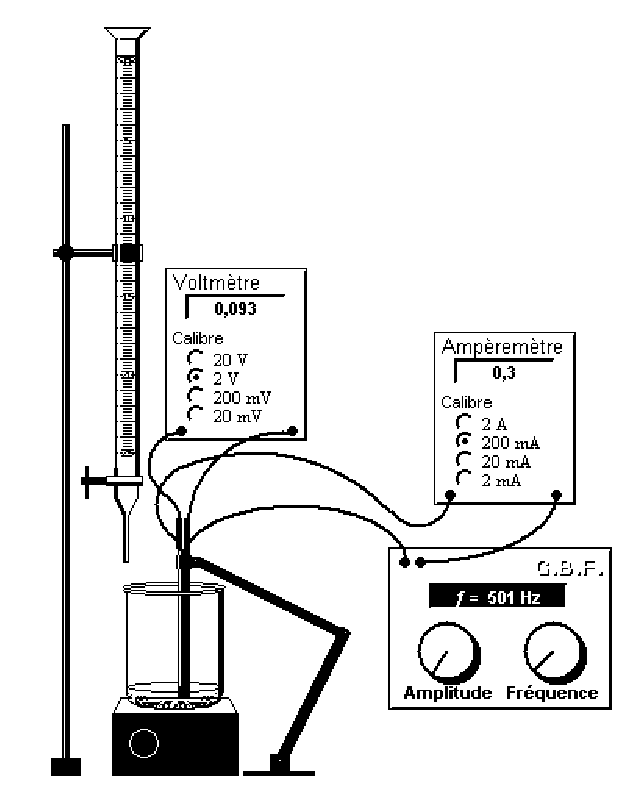
\includegraphics[width=6cm]{tp_prem_s_chimie/tp6_determination_par_conductimetrie_concentration/montage_conductimetrie.png.eps}
\caption{Dispositif exp�rimental}
\end{figure}
\end{center}


\end{multicols}



\subsection{R�sultats}
\begin{enumerate}
\item Calculer la conductance $G$ et compl�ter le tableau suivant.

\begin{arraydata}{6}
\hline
$V_0$ ($mL$)       &  0 &  5 & 10 & 15 & 20 & 25 \\ \hline
\rule[-0.4cm]{0cm}{1cm}
$C$ ($mol.L^{-1}$) &    &    &    &    &    &    \\ \hline
\rule[-0.4cm]{0cm}{1cm}
$G$ ($mS$)         &    &    &    &    &    &    \\ \hline
\end{arraydata}

\item Tracer la courbe d'�talonnage $G = f (C)$.
\end{enumerate}



\pagebreak
%\newpage


\section{D�termination de la concentration en $NaCl$ d'une solution de
  s�rum physiologique}

L'objectif est de d�terminer la concentration du chlorure de sodium dans le s�rum physiologique injectable.

\begin{enumerate}
\item Diluer au $1/100\ieme$ le s�rum physiologique. En pr�parer $500~mL$.

\item D�crire � l'aide de sch�mas le protocole utilis� pour r�aliser
  cette dilution au $1/100\ieme$ et obtenir la solution $S'$.

\item D�terminer la conductance $G'$ de cette solution $S'$.

\item En d�duire la concentration $C'$ du chlorure de sodium dans le
  s�rum physiologique dilu�.

\end{enumerate}


\vressort{3}

\section{Questions compl�mentaires}

%\begin{multicols}{2}

\begin{enumerate}
\item Expliquer comment calculer la concentration $C$ des diff�rentes
  solutions de chlorure de sodium. Donner l'expression de $C$ en
  fonction de $C_0$, $V_0$, $V$.


\item Comment calcule-t-on la conductance $G$ ?

\item Pour quelle raison pratique a-t-on int�r�t � prendre $U =
  1,00~V$ dans les diff�rentes manipulations ?

\item En extrapolant la courbe d'�talonnage, pr�voir la conductance
  d'une portion de solution concentr�e � $T = 58,4~g.L^{-1}$. Mesurer
  la conductance r�elle d'une portion d'une telle solution. Que
  peut-on conclure quant � la m�thode d'�talonnage utilis�e. On donne
  $M_{Na} = 23~g.mol^{-1}$ et $M_{Cl} = 35,5~g.mol^{-1}$.

\item Rappeler la valeur de la concentration $C'$ du chlorure de
  sodium dans le s�rum physiologique dilu�.

\item Comment peut-on alors d�terminer la concentration $C_0'$ du
  chlorure de sodium dans la solution commerciale de s�rum
  physiologique ? Calculer cette concentration $C_0'$ puis le titre
  massique (concentration massique) correspondant $T_0$. Le comparer avec
  les indications figurant sur l'�tiquette du flacon ($0,9~\%$ en masse).
\end{enumerate}


%\vressort{1}
\vressort{3}

\begin{center}
\begin{figure}[H]
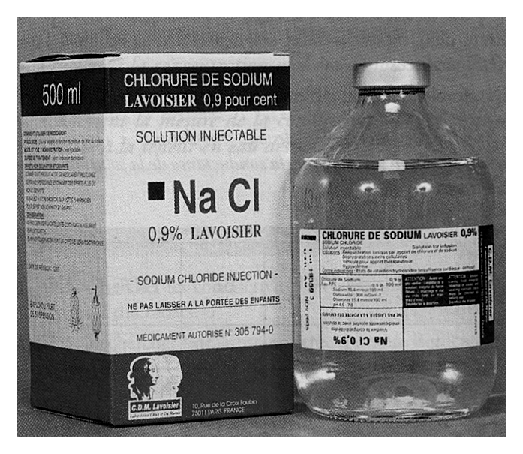
\includegraphics[width=7cm]{tp_prem_s_chimie/tp6_determination_par_conductimetrie_concentration/solution_nacl.png.eps}
\caption{Solution de chlorure de sodium}
\end{figure}
\end{center}


%\end{multicols}


\vressort{3} % tp caract�ristique d'un
                                % r�cepteur (�lectrolyseur)


\tp{D�termination par conductim�trie\\
de la concentration en solut�\\
d'une solution ionique}


\begin{multicols}{2}

\objectifs{
\item r�aliser une courbe d'�talonnage $G = f(C)$ et en d�duire une
  concentration inconnue.
\item Aborder une limite de la m�thode d'�talonnage.
}
\vspace*{2cm}


\materiel{
\item b�cher $600~mL$
\item fiole jaug�e $500~mL$
\item burette gradu�e $25~mL$
\item pipette jaug�e $5~mL$
\item agitateur magn�tique.
\item solution de chlorure de sodium $S_0$ de concentration $C_0 =
  0,10~mol.L^{-1}$
\item flacon de s�rum physiologique
\item eau d�min�ralis�e
\item g�n�rateur basse fr�quence.
\item 2 multim�tres
\item cellule de conductim�trie.
}


\end{multicols}




\section{R�alisation d'une �chelle de conductance}


\begin{multicols}{2}

\subsection{Protocole op�ratoire}
\begin{enumerate}
\item Rincer la burette, la remplir � l'aide de la solution $S_0$ ajuster le
z�ro.

\item Avec la fiole jaug�e, introduire $V = 500~mL$ d'eau d�min�ralis�e dans
le b�cher.

\item Placer la cellule conductim�trique dans le b�cher et r�aliser le
montage �lectrique correspondant au sch�ma ci-contre. Les 2
multim�tres sont en mode alternatif ($AC$ ou \acsymbol).

\item Sur le GBF, r�gler la fr�quence $500~Hz$ et fixer la tension �
$1,00~V$.

\item Au contenu du b�cher, ajouter les volumes $V_0$ suivants de solution
de chlorure de sodium mesur�s pr�cis�ment gr�ce � la burette. Apr�s
chaque addition, v�rifier que la tension est toujours de $1,00~V$ et
relever la valeur de l'intensit�.

\end{enumerate}




\begin{center}
\begin{figure}[H]
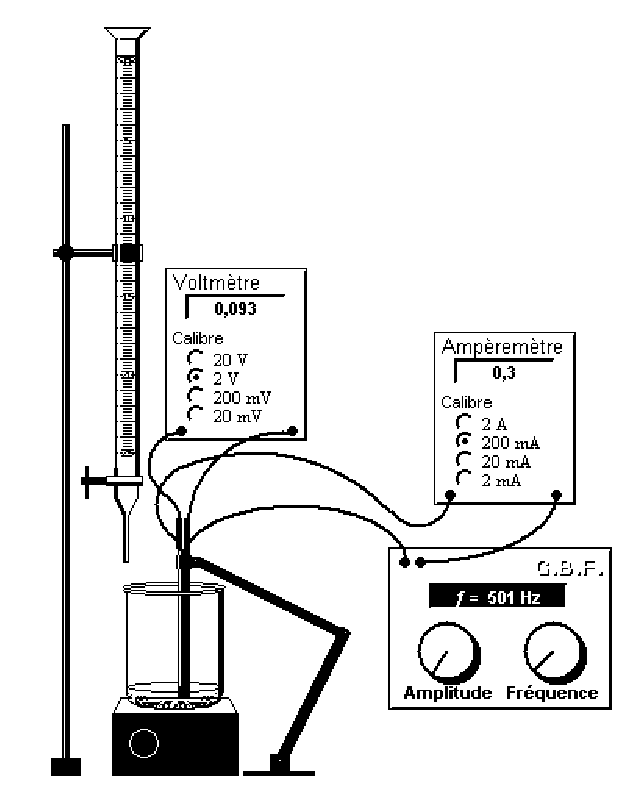
\includegraphics[width=6cm]{tp_prem_s_chimie/tp6_determination_par_conductimetrie_concentration/montage_conductimetrie.png.eps}
\caption{Dispositif exp�rimental}
\end{figure}
\end{center}


\end{multicols}



\subsection{R�sultats}
\begin{enumerate}
\item Calculer la conductance $G$ et compl�ter le tableau suivant.

\begin{arraydata}{6}
\hline
$V_0$ ($mL$)       &  0 &  5 & 10 & 15 & 20 & 25 \\ \hline
\rule[-0.4cm]{0cm}{1cm}
$C$ ($mol.L^{-1}$) &    &    &    &    &    &    \\ \hline
\rule[-0.4cm]{0cm}{1cm}
$G$ ($mS$)         &    &    &    &    &    &    \\ \hline
\end{arraydata}

\item Tracer la courbe d'�talonnage $G = f (C)$.
\end{enumerate}



\pagebreak
%\newpage


\section{D�termination de la concentration en $NaCl$ d'une solution de
  s�rum physiologique}

L'objectif est de d�terminer la concentration du chlorure de sodium dans le s�rum physiologique injectable.

\begin{enumerate}
\item Diluer au $1/100\ieme$ le s�rum physiologique. En pr�parer $500~mL$.

\item D�crire � l'aide de sch�mas le protocole utilis� pour r�aliser
  cette dilution au $1/100\ieme$ et obtenir la solution $S'$.

\item D�terminer la conductance $G'$ de cette solution $S'$.

\item En d�duire la concentration $C'$ du chlorure de sodium dans le
  s�rum physiologique dilu�.

\end{enumerate}


\vressort{3}

\section{Questions compl�mentaires}

%\begin{multicols}{2}

\begin{enumerate}
\item Expliquer comment calculer la concentration $C$ des diff�rentes
  solutions de chlorure de sodium. Donner l'expression de $C$ en
  fonction de $C_0$, $V_0$, $V$.


\item Comment calcule-t-on la conductance $G$ ?

\item Pour quelle raison pratique a-t-on int�r�t � prendre $U =
  1,00~V$ dans les diff�rentes manipulations ?

\item En extrapolant la courbe d'�talonnage, pr�voir la conductance
  d'une portion de solution concentr�e � $T = 58,4~g.L^{-1}$. Mesurer
  la conductance r�elle d'une portion d'une telle solution. Que
  peut-on conclure quant � la m�thode d'�talonnage utilis�e. On donne
  $M_{Na} = 23~g.mol^{-1}$ et $M_{Cl} = 35,5~g.mol^{-1}$.

\item Rappeler la valeur de la concentration $C'$ du chlorure de
  sodium dans le s�rum physiologique dilu�.

\item Comment peut-on alors d�terminer la concentration $C_0'$ du
  chlorure de sodium dans la solution commerciale de s�rum
  physiologique ? Calculer cette concentration $C_0'$ puis le titre
  massique (concentration massique) correspondant $T_0$. Le comparer avec
  les indications figurant sur l'�tiquette du flacon ($0,9~\%$ en masse).
\end{enumerate}


%\vressort{1}
\vressort{3}

\begin{center}
\begin{figure}[H]
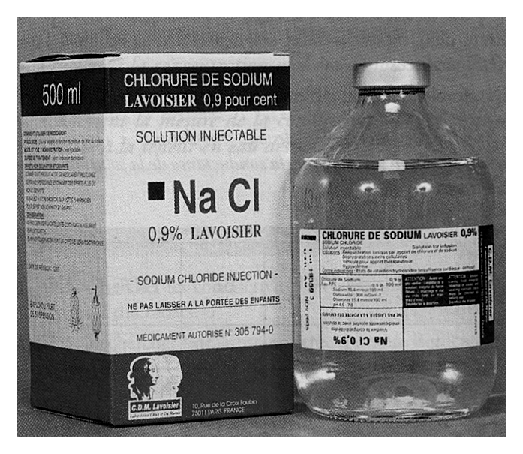
\includegraphics[width=7cm]{tp_prem_s_chimie/tp6_determination_par_conductimetrie_concentration/solution_nacl.png.eps}
\caption{Solution de chlorure de sodium}
\end{figure}
\end{center}


%\end{multicols}


\vressort{3} % tp puissance �nergie (continu)





% % tp caract�ristique d'un r�cepteur (moteur � courant continu)

% % potentiel le long d'un circuit �lectrique 
% % tp �tude du montage potentiom�trique (diviseur de tension)

% % tp �tude de la diode PN
% % tp �tude de la diode Zener
% % tp �tude d'un r�gulateur int�gr� de tension 7805



% % tp th�or�me de th�venin / norton
% % tp th�or�me de superposition
% % tp ao en regime lineaire
% % tp ao en r�gime non lineaire


\chapitre{R�gimes variables}
\tp{D�termination par conductim�trie\\
de la concentration en solut�\\
d'une solution ionique}


\begin{multicols}{2}

\objectifs{
\item r�aliser une courbe d'�talonnage $G = f(C)$ et en d�duire une
  concentration inconnue.
\item Aborder une limite de la m�thode d'�talonnage.
}
\vspace*{2cm}


\materiel{
\item b�cher $600~mL$
\item fiole jaug�e $500~mL$
\item burette gradu�e $25~mL$
\item pipette jaug�e $5~mL$
\item agitateur magn�tique.
\item solution de chlorure de sodium $S_0$ de concentration $C_0 =
  0,10~mol.L^{-1}$
\item flacon de s�rum physiologique
\item eau d�min�ralis�e
\item g�n�rateur basse fr�quence.
\item 2 multim�tres
\item cellule de conductim�trie.
}


\end{multicols}




\section{R�alisation d'une �chelle de conductance}


\begin{multicols}{2}

\subsection{Protocole op�ratoire}
\begin{enumerate}
\item Rincer la burette, la remplir � l'aide de la solution $S_0$ ajuster le
z�ro.

\item Avec la fiole jaug�e, introduire $V = 500~mL$ d'eau d�min�ralis�e dans
le b�cher.

\item Placer la cellule conductim�trique dans le b�cher et r�aliser le
montage �lectrique correspondant au sch�ma ci-contre. Les 2
multim�tres sont en mode alternatif ($AC$ ou \acsymbol).

\item Sur le GBF, r�gler la fr�quence $500~Hz$ et fixer la tension �
$1,00~V$.

\item Au contenu du b�cher, ajouter les volumes $V_0$ suivants de solution
de chlorure de sodium mesur�s pr�cis�ment gr�ce � la burette. Apr�s
chaque addition, v�rifier que la tension est toujours de $1,00~V$ et
relever la valeur de l'intensit�.

\end{enumerate}




\begin{center}
\begin{figure}[H]
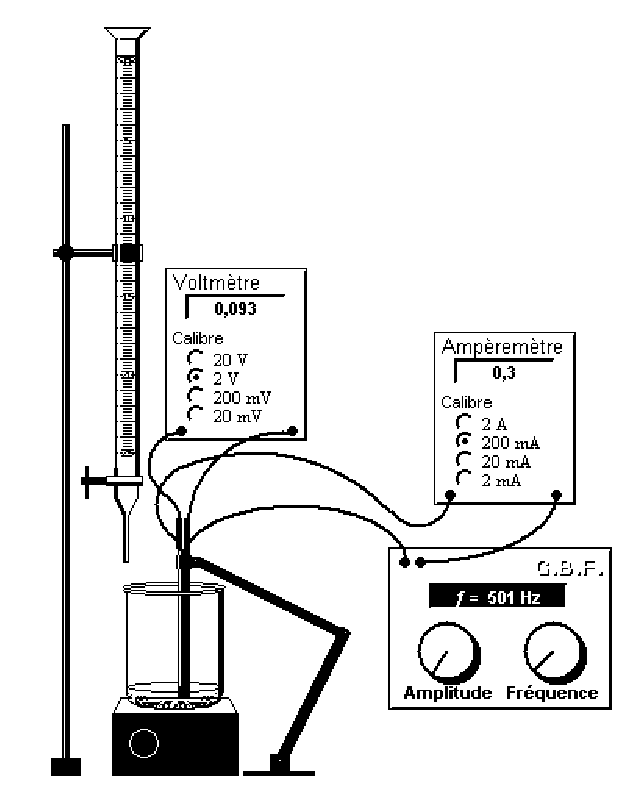
\includegraphics[width=6cm]{tp_prem_s_chimie/tp6_determination_par_conductimetrie_concentration/montage_conductimetrie.png.eps}
\caption{Dispositif exp�rimental}
\end{figure}
\end{center}


\end{multicols}



\subsection{R�sultats}
\begin{enumerate}
\item Calculer la conductance $G$ et compl�ter le tableau suivant.

\begin{arraydata}{6}
\hline
$V_0$ ($mL$)       &  0 &  5 & 10 & 15 & 20 & 25 \\ \hline
\rule[-0.4cm]{0cm}{1cm}
$C$ ($mol.L^{-1}$) &    &    &    &    &    &    \\ \hline
\rule[-0.4cm]{0cm}{1cm}
$G$ ($mS$)         &    &    &    &    &    &    \\ \hline
\end{arraydata}

\item Tracer la courbe d'�talonnage $G = f (C)$.
\end{enumerate}



\pagebreak
%\newpage


\section{D�termination de la concentration en $NaCl$ d'une solution de
  s�rum physiologique}

L'objectif est de d�terminer la concentration du chlorure de sodium dans le s�rum physiologique injectable.

\begin{enumerate}
\item Diluer au $1/100\ieme$ le s�rum physiologique. En pr�parer $500~mL$.

\item D�crire � l'aide de sch�mas le protocole utilis� pour r�aliser
  cette dilution au $1/100\ieme$ et obtenir la solution $S'$.

\item D�terminer la conductance $G'$ de cette solution $S'$.

\item En d�duire la concentration $C'$ du chlorure de sodium dans le
  s�rum physiologique dilu�.

\end{enumerate}


\vressort{3}

\section{Questions compl�mentaires}

%\begin{multicols}{2}

\begin{enumerate}
\item Expliquer comment calculer la concentration $C$ des diff�rentes
  solutions de chlorure de sodium. Donner l'expression de $C$ en
  fonction de $C_0$, $V_0$, $V$.


\item Comment calcule-t-on la conductance $G$ ?

\item Pour quelle raison pratique a-t-on int�r�t � prendre $U =
  1,00~V$ dans les diff�rentes manipulations ?

\item En extrapolant la courbe d'�talonnage, pr�voir la conductance
  d'une portion de solution concentr�e � $T = 58,4~g.L^{-1}$. Mesurer
  la conductance r�elle d'une portion d'une telle solution. Que
  peut-on conclure quant � la m�thode d'�talonnage utilis�e. On donne
  $M_{Na} = 23~g.mol^{-1}$ et $M_{Cl} = 35,5~g.mol^{-1}$.

\item Rappeler la valeur de la concentration $C'$ du chlorure de
  sodium dans le s�rum physiologique dilu�.

\item Comment peut-on alors d�terminer la concentration $C_0'$ du
  chlorure de sodium dans la solution commerciale de s�rum
  physiologique ? Calculer cette concentration $C_0'$ puis le titre
  massique (concentration massique) correspondant $T_0$. Le comparer avec
  les indications figurant sur l'�tiquette du flacon ($0,9~\%$ en masse).
\end{enumerate}


%\vressort{1}
\vressort{3}

\begin{center}
\begin{figure}[H]
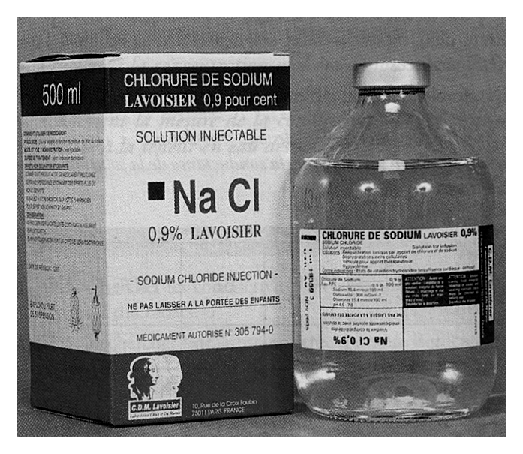
\includegraphics[width=7cm]{tp_prem_s_chimie/tp6_determination_par_conductimetrie_concentration/solution_nacl.png.eps}
\caption{Solution de chlorure de sodium}
\end{figure}
\end{center}


%\end{multicols}


\vressort{3} % tp regime variable, oscillo, gbf
\tp{D�termination par conductim�trie\\
de la concentration en solut�\\
d'une solution ionique}


\begin{multicols}{2}

\objectifs{
\item r�aliser une courbe d'�talonnage $G = f(C)$ et en d�duire une
  concentration inconnue.
\item Aborder une limite de la m�thode d'�talonnage.
}
\vspace*{2cm}


\materiel{
\item b�cher $600~mL$
\item fiole jaug�e $500~mL$
\item burette gradu�e $25~mL$
\item pipette jaug�e $5~mL$
\item agitateur magn�tique.
\item solution de chlorure de sodium $S_0$ de concentration $C_0 =
  0,10~mol.L^{-1}$
\item flacon de s�rum physiologique
\item eau d�min�ralis�e
\item g�n�rateur basse fr�quence.
\item 2 multim�tres
\item cellule de conductim�trie.
}


\end{multicols}




\section{R�alisation d'une �chelle de conductance}


\begin{multicols}{2}

\subsection{Protocole op�ratoire}
\begin{enumerate}
\item Rincer la burette, la remplir � l'aide de la solution $S_0$ ajuster le
z�ro.

\item Avec la fiole jaug�e, introduire $V = 500~mL$ d'eau d�min�ralis�e dans
le b�cher.

\item Placer la cellule conductim�trique dans le b�cher et r�aliser le
montage �lectrique correspondant au sch�ma ci-contre. Les 2
multim�tres sont en mode alternatif ($AC$ ou \acsymbol).

\item Sur le GBF, r�gler la fr�quence $500~Hz$ et fixer la tension �
$1,00~V$.

\item Au contenu du b�cher, ajouter les volumes $V_0$ suivants de solution
de chlorure de sodium mesur�s pr�cis�ment gr�ce � la burette. Apr�s
chaque addition, v�rifier que la tension est toujours de $1,00~V$ et
relever la valeur de l'intensit�.

\end{enumerate}




\begin{center}
\begin{figure}[H]
\includegraphics[width=6cm]{tp_prem_s_chimie/tp6_determination_par_conductimetrie_concentration/montage_conductimetrie.png.eps}
\caption{Dispositif exp�rimental}
\end{figure}
\end{center}


\end{multicols}



\subsection{R�sultats}
\begin{enumerate}
\item Calculer la conductance $G$ et compl�ter le tableau suivant.

\begin{arraydata}{6}
\hline
$V_0$ ($mL$)       &  0 &  5 & 10 & 15 & 20 & 25 \\ \hline
\rule[-0.4cm]{0cm}{1cm}
$C$ ($mol.L^{-1}$) &    &    &    &    &    &    \\ \hline
\rule[-0.4cm]{0cm}{1cm}
$G$ ($mS$)         &    &    &    &    &    &    \\ \hline
\end{arraydata}

\item Tracer la courbe d'�talonnage $G = f (C)$.
\end{enumerate}



\pagebreak
%\newpage


\section{D�termination de la concentration en $NaCl$ d'une solution de
  s�rum physiologique}

L'objectif est de d�terminer la concentration du chlorure de sodium dans le s�rum physiologique injectable.

\begin{enumerate}
\item Diluer au $1/100\ieme$ le s�rum physiologique. En pr�parer $500~mL$.

\item D�crire � l'aide de sch�mas le protocole utilis� pour r�aliser
  cette dilution au $1/100\ieme$ et obtenir la solution $S'$.

\item D�terminer la conductance $G'$ de cette solution $S'$.

\item En d�duire la concentration $C'$ du chlorure de sodium dans le
  s�rum physiologique dilu�.

\end{enumerate}


\vressort{3}

\section{Questions compl�mentaires}

%\begin{multicols}{2}

\begin{enumerate}
\item Expliquer comment calculer la concentration $C$ des diff�rentes
  solutions de chlorure de sodium. Donner l'expression de $C$ en
  fonction de $C_0$, $V_0$, $V$.


\item Comment calcule-t-on la conductance $G$ ?

\item Pour quelle raison pratique a-t-on int�r�t � prendre $U =
  1,00~V$ dans les diff�rentes manipulations ?

\item En extrapolant la courbe d'�talonnage, pr�voir la conductance
  d'une portion de solution concentr�e � $T = 58,4~g.L^{-1}$. Mesurer
  la conductance r�elle d'une portion d'une telle solution. Que
  peut-on conclure quant � la m�thode d'�talonnage utilis�e. On donne
  $M_{Na} = 23~g.mol^{-1}$ et $M_{Cl} = 35,5~g.mol^{-1}$.

\item Rappeler la valeur de la concentration $C'$ du chlorure de
  sodium dans le s�rum physiologique dilu�.

\item Comment peut-on alors d�terminer la concentration $C_0'$ du
  chlorure de sodium dans la solution commerciale de s�rum
  physiologique ? Calculer cette concentration $C_0'$ puis le titre
  massique (concentration massique) correspondant $T_0$. Le comparer avec
  les indications figurant sur l'�tiquette du flacon ($0,9~\%$ en masse).
\end{enumerate}


%\vressort{1}
\vressort{3}

\begin{center}
\begin{figure}[H]
\includegraphics[width=7cm]{tp_prem_s_chimie/tp6_determination_par_conductimetrie_concentration/solution_nacl.png.eps}
\caption{Solution de chlorure de sodium}
\end{figure}
\end{center}


%\end{multicols}


\vressort{3}
\tp{D�termination par conductim�trie\\
de la concentration en solut�\\
d'une solution ionique}


\begin{multicols}{2}

\objectifs{
\item r�aliser une courbe d'�talonnage $G = f(C)$ et en d�duire une
  concentration inconnue.
\item Aborder une limite de la m�thode d'�talonnage.
}
\vspace*{2cm}


\materiel{
\item b�cher $600~mL$
\item fiole jaug�e $500~mL$
\item burette gradu�e $25~mL$
\item pipette jaug�e $5~mL$
\item agitateur magn�tique.
\item solution de chlorure de sodium $S_0$ de concentration $C_0 =
  0,10~mol.L^{-1}$
\item flacon de s�rum physiologique
\item eau d�min�ralis�e
\item g�n�rateur basse fr�quence.
\item 2 multim�tres
\item cellule de conductim�trie.
}


\end{multicols}




\section{R�alisation d'une �chelle de conductance}


\begin{multicols}{2}

\subsection{Protocole op�ratoire}
\begin{enumerate}
\item Rincer la burette, la remplir � l'aide de la solution $S_0$ ajuster le
z�ro.

\item Avec la fiole jaug�e, introduire $V = 500~mL$ d'eau d�min�ralis�e dans
le b�cher.

\item Placer la cellule conductim�trique dans le b�cher et r�aliser le
montage �lectrique correspondant au sch�ma ci-contre. Les 2
multim�tres sont en mode alternatif ($AC$ ou \acsymbol).

\item Sur le GBF, r�gler la fr�quence $500~Hz$ et fixer la tension �
$1,00~V$.

\item Au contenu du b�cher, ajouter les volumes $V_0$ suivants de solution
de chlorure de sodium mesur�s pr�cis�ment gr�ce � la burette. Apr�s
chaque addition, v�rifier que la tension est toujours de $1,00~V$ et
relever la valeur de l'intensit�.

\end{enumerate}




\begin{center}
\begin{figure}[H]
\includegraphics[width=6cm]{tp_prem_s_chimie/tp6_determination_par_conductimetrie_concentration/montage_conductimetrie.png.eps}
\caption{Dispositif exp�rimental}
\end{figure}
\end{center}


\end{multicols}



\subsection{R�sultats}
\begin{enumerate}
\item Calculer la conductance $G$ et compl�ter le tableau suivant.

\begin{arraydata}{6}
\hline
$V_0$ ($mL$)       &  0 &  5 & 10 & 15 & 20 & 25 \\ \hline
\rule[-0.4cm]{0cm}{1cm}
$C$ ($mol.L^{-1}$) &    &    &    &    &    &    \\ \hline
\rule[-0.4cm]{0cm}{1cm}
$G$ ($mS$)         &    &    &    &    &    &    \\ \hline
\end{arraydata}

\item Tracer la courbe d'�talonnage $G = f (C)$.
\end{enumerate}



\pagebreak
%\newpage


\section{D�termination de la concentration en $NaCl$ d'une solution de
  s�rum physiologique}

L'objectif est de d�terminer la concentration du chlorure de sodium dans le s�rum physiologique injectable.

\begin{enumerate}
\item Diluer au $1/100\ieme$ le s�rum physiologique. En pr�parer $500~mL$.

\item D�crire � l'aide de sch�mas le protocole utilis� pour r�aliser
  cette dilution au $1/100\ieme$ et obtenir la solution $S'$.

\item D�terminer la conductance $G'$ de cette solution $S'$.

\item En d�duire la concentration $C'$ du chlorure de sodium dans le
  s�rum physiologique dilu�.

\end{enumerate}


\vressort{3}

\section{Questions compl�mentaires}

%\begin{multicols}{2}

\begin{enumerate}
\item Expliquer comment calculer la concentration $C$ des diff�rentes
  solutions de chlorure de sodium. Donner l'expression de $C$ en
  fonction de $C_0$, $V_0$, $V$.


\item Comment calcule-t-on la conductance $G$ ?

\item Pour quelle raison pratique a-t-on int�r�t � prendre $U =
  1,00~V$ dans les diff�rentes manipulations ?

\item En extrapolant la courbe d'�talonnage, pr�voir la conductance
  d'une portion de solution concentr�e � $T = 58,4~g.L^{-1}$. Mesurer
  la conductance r�elle d'une portion d'une telle solution. Que
  peut-on conclure quant � la m�thode d'�talonnage utilis�e. On donne
  $M_{Na} = 23~g.mol^{-1}$ et $M_{Cl} = 35,5~g.mol^{-1}$.

\item Rappeler la valeur de la concentration $C'$ du chlorure de
  sodium dans le s�rum physiologique dilu�.

\item Comment peut-on alors d�terminer la concentration $C_0'$ du
  chlorure de sodium dans la solution commerciale de s�rum
  physiologique ? Calculer cette concentration $C_0'$ puis le titre
  massique (concentration massique) correspondant $T_0$. Le comparer avec
  les indications figurant sur l'�tiquette du flacon ($0,9~\%$ en masse).
\end{enumerate}


%\vressort{1}
\vressort{3}

\begin{center}
\begin{figure}[H]
\includegraphics[width=7cm]{tp_prem_s_chimie/tp6_determination_par_conductimetrie_concentration/solution_nacl.png.eps}
\caption{Solution de chlorure de sodium}
\end{figure}
\end{center}


%\end{multicols}


\vressort{3} % cours grandeurs p�riodiques
\tp{D�termination par conductim�trie\\
de la concentration en solut�\\
d'une solution ionique}


\begin{multicols}{2}

\objectifs{
\item r�aliser une courbe d'�talonnage $G = f(C)$ et en d�duire une
  concentration inconnue.
\item Aborder une limite de la m�thode d'�talonnage.
}
\vspace*{2cm}


\materiel{
\item b�cher $600~mL$
\item fiole jaug�e $500~mL$
\item burette gradu�e $25~mL$
\item pipette jaug�e $5~mL$
\item agitateur magn�tique.
\item solution de chlorure de sodium $S_0$ de concentration $C_0 =
  0,10~mol.L^{-1}$
\item flacon de s�rum physiologique
\item eau d�min�ralis�e
\item g�n�rateur basse fr�quence.
\item 2 multim�tres
\item cellule de conductim�trie.
}


\end{multicols}




\section{R�alisation d'une �chelle de conductance}


\begin{multicols}{2}

\subsection{Protocole op�ratoire}
\begin{enumerate}
\item Rincer la burette, la remplir � l'aide de la solution $S_0$ ajuster le
z�ro.

\item Avec la fiole jaug�e, introduire $V = 500~mL$ d'eau d�min�ralis�e dans
le b�cher.

\item Placer la cellule conductim�trique dans le b�cher et r�aliser le
montage �lectrique correspondant au sch�ma ci-contre. Les 2
multim�tres sont en mode alternatif ($AC$ ou \acsymbol).

\item Sur le GBF, r�gler la fr�quence $500~Hz$ et fixer la tension �
$1,00~V$.

\item Au contenu du b�cher, ajouter les volumes $V_0$ suivants de solution
de chlorure de sodium mesur�s pr�cis�ment gr�ce � la burette. Apr�s
chaque addition, v�rifier que la tension est toujours de $1,00~V$ et
relever la valeur de l'intensit�.

\end{enumerate}




\begin{center}
\begin{figure}[H]
\includegraphics[width=6cm]{tp_prem_s_chimie/tp6_determination_par_conductimetrie_concentration/montage_conductimetrie.png.eps}
\caption{Dispositif exp�rimental}
\end{figure}
\end{center}


\end{multicols}



\subsection{R�sultats}
\begin{enumerate}
\item Calculer la conductance $G$ et compl�ter le tableau suivant.

\begin{arraydata}{6}
\hline
$V_0$ ($mL$)       &  0 &  5 & 10 & 15 & 20 & 25 \\ \hline
\rule[-0.4cm]{0cm}{1cm}
$C$ ($mol.L^{-1}$) &    &    &    &    &    &    \\ \hline
\rule[-0.4cm]{0cm}{1cm}
$G$ ($mS$)         &    &    &    &    &    &    \\ \hline
\end{arraydata}

\item Tracer la courbe d'�talonnage $G = f (C)$.
\end{enumerate}



\pagebreak
%\newpage


\section{D�termination de la concentration en $NaCl$ d'une solution de
  s�rum physiologique}

L'objectif est de d�terminer la concentration du chlorure de sodium dans le s�rum physiologique injectable.

\begin{enumerate}
\item Diluer au $1/100\ieme$ le s�rum physiologique. En pr�parer $500~mL$.

\item D�crire � l'aide de sch�mas le protocole utilis� pour r�aliser
  cette dilution au $1/100\ieme$ et obtenir la solution $S'$.

\item D�terminer la conductance $G'$ de cette solution $S'$.

\item En d�duire la concentration $C'$ du chlorure de sodium dans le
  s�rum physiologique dilu�.

\end{enumerate}


\vressort{3}

\section{Questions compl�mentaires}

%\begin{multicols}{2}

\begin{enumerate}
\item Expliquer comment calculer la concentration $C$ des diff�rentes
  solutions de chlorure de sodium. Donner l'expression de $C$ en
  fonction de $C_0$, $V_0$, $V$.


\item Comment calcule-t-on la conductance $G$ ?

\item Pour quelle raison pratique a-t-on int�r�t � prendre $U =
  1,00~V$ dans les diff�rentes manipulations ?

\item En extrapolant la courbe d'�talonnage, pr�voir la conductance
  d'une portion de solution concentr�e � $T = 58,4~g.L^{-1}$. Mesurer
  la conductance r�elle d'une portion d'une telle solution. Que
  peut-on conclure quant � la m�thode d'�talonnage utilis�e. On donne
  $M_{Na} = 23~g.mol^{-1}$ et $M_{Cl} = 35,5~g.mol^{-1}$.

\item Rappeler la valeur de la concentration $C'$ du chlorure de
  sodium dans le s�rum physiologique dilu�.

\item Comment peut-on alors d�terminer la concentration $C_0'$ du
  chlorure de sodium dans la solution commerciale de s�rum
  physiologique ? Calculer cette concentration $C_0'$ puis le titre
  massique (concentration massique) correspondant $T_0$. Le comparer avec
  les indications figurant sur l'�tiquette du flacon ($0,9~\%$ en masse).
\end{enumerate}


%\vressort{1}
\vressort{3}

\begin{center}
\begin{figure}[H]
\includegraphics[width=7cm]{tp_prem_s_chimie/tp6_determination_par_conductimetrie_concentration/solution_nacl.png.eps}
\caption{Solution de chlorure de sodium}
\end{figure}
\end{center}


%\end{multicols}


\vressort{3} % cours r�gimes transitoires


% tp transfo, pont de diode, filtrage C, RIT


% tp force �lectromagn�tique (balance �lectromagn�tique ou haut-parleur)

% tp Charge � courant constant d'un condensateur

% tp transistor bipolaire (caract�ristiques)
% tp transistor bipolaire (utilisations)
% tp transistor bipolaire (commutation)

% tp champ magn�tique
% tp r�gime transitoire RC et RL
% tp r�gime transitoire RLC

% tp utilisation du gbf et de l'oscillo
% tp mesure de valeur moyenne et de valeur efficace d'un signal p�riodique



\tp{D�termination par conductim�trie\\
de la concentration en solut�\\
d'une solution ionique}


\begin{multicols}{2}

\objectifs{
\item r�aliser une courbe d'�talonnage $G = f(C)$ et en d�duire une
  concentration inconnue.
\item Aborder une limite de la m�thode d'�talonnage.
}
\vspace*{2cm}


\materiel{
\item b�cher $600~mL$
\item fiole jaug�e $500~mL$
\item burette gradu�e $25~mL$
\item pipette jaug�e $5~mL$
\item agitateur magn�tique.
\item solution de chlorure de sodium $S_0$ de concentration $C_0 =
  0,10~mol.L^{-1}$
\item flacon de s�rum physiologique
\item eau d�min�ralis�e
\item g�n�rateur basse fr�quence.
\item 2 multim�tres
\item cellule de conductim�trie.
}


\end{multicols}




\section{R�alisation d'une �chelle de conductance}


\begin{multicols}{2}

\subsection{Protocole op�ratoire}
\begin{enumerate}
\item Rincer la burette, la remplir � l'aide de la solution $S_0$ ajuster le
z�ro.

\item Avec la fiole jaug�e, introduire $V = 500~mL$ d'eau d�min�ralis�e dans
le b�cher.

\item Placer la cellule conductim�trique dans le b�cher et r�aliser le
montage �lectrique correspondant au sch�ma ci-contre. Les 2
multim�tres sont en mode alternatif ($AC$ ou \acsymbol).

\item Sur le GBF, r�gler la fr�quence $500~Hz$ et fixer la tension �
$1,00~V$.

\item Au contenu du b�cher, ajouter les volumes $V_0$ suivants de solution
de chlorure de sodium mesur�s pr�cis�ment gr�ce � la burette. Apr�s
chaque addition, v�rifier que la tension est toujours de $1,00~V$ et
relever la valeur de l'intensit�.

\end{enumerate}




\begin{center}
\begin{figure}[H]
\includegraphics[width=6cm]{tp_prem_s_chimie/tp6_determination_par_conductimetrie_concentration/montage_conductimetrie.png.eps}
\caption{Dispositif exp�rimental}
\end{figure}
\end{center}


\end{multicols}



\subsection{R�sultats}
\begin{enumerate}
\item Calculer la conductance $G$ et compl�ter le tableau suivant.

\begin{arraydata}{6}
\hline
$V_0$ ($mL$)       &  0 &  5 & 10 & 15 & 20 & 25 \\ \hline
\rule[-0.4cm]{0cm}{1cm}
$C$ ($mol.L^{-1}$) &    &    &    &    &    &    \\ \hline
\rule[-0.4cm]{0cm}{1cm}
$G$ ($mS$)         &    &    &    &    &    &    \\ \hline
\end{arraydata}

\item Tracer la courbe d'�talonnage $G = f (C)$.
\end{enumerate}



\pagebreak
%\newpage


\section{D�termination de la concentration en $NaCl$ d'une solution de
  s�rum physiologique}

L'objectif est de d�terminer la concentration du chlorure de sodium dans le s�rum physiologique injectable.

\begin{enumerate}
\item Diluer au $1/100\ieme$ le s�rum physiologique. En pr�parer $500~mL$.

\item D�crire � l'aide de sch�mas le protocole utilis� pour r�aliser
  cette dilution au $1/100\ieme$ et obtenir la solution $S'$.

\item D�terminer la conductance $G'$ de cette solution $S'$.

\item En d�duire la concentration $C'$ du chlorure de sodium dans le
  s�rum physiologique dilu�.

\end{enumerate}


\vressort{3}

\section{Questions compl�mentaires}

%\begin{multicols}{2}

\begin{enumerate}
\item Expliquer comment calculer la concentration $C$ des diff�rentes
  solutions de chlorure de sodium. Donner l'expression de $C$ en
  fonction de $C_0$, $V_0$, $V$.


\item Comment calcule-t-on la conductance $G$ ?

\item Pour quelle raison pratique a-t-on int�r�t � prendre $U =
  1,00~V$ dans les diff�rentes manipulations ?

\item En extrapolant la courbe d'�talonnage, pr�voir la conductance
  d'une portion de solution concentr�e � $T = 58,4~g.L^{-1}$. Mesurer
  la conductance r�elle d'une portion d'une telle solution. Que
  peut-on conclure quant � la m�thode d'�talonnage utilis�e. On donne
  $M_{Na} = 23~g.mol^{-1}$ et $M_{Cl} = 35,5~g.mol^{-1}$.

\item Rappeler la valeur de la concentration $C'$ du chlorure de
  sodium dans le s�rum physiologique dilu�.

\item Comment peut-on alors d�terminer la concentration $C_0'$ du
  chlorure de sodium dans la solution commerciale de s�rum
  physiologique ? Calculer cette concentration $C_0'$ puis le titre
  massique (concentration massique) correspondant $T_0$. Le comparer avec
  les indications figurant sur l'�tiquette du flacon ($0,9~\%$ en masse).
\end{enumerate}


%\vressort{1}
\vressort{3}

\begin{center}
\begin{figure}[H]
\includegraphics[width=7cm]{tp_prem_s_chimie/tp6_determination_par_conductimetrie_concentration/solution_nacl.png.eps}
\caption{Solution de chlorure de sodium}
\end{figure}
\end{center}


%\end{multicols}


\vressort{3} % cours r�gimes sinuso�daux
\tp{D�termination par conductim�trie\\
de la concentration en solut�\\
d'une solution ionique}


\begin{multicols}{2}

\objectifs{
\item r�aliser une courbe d'�talonnage $G = f(C)$ et en d�duire une
  concentration inconnue.
\item Aborder une limite de la m�thode d'�talonnage.
}
\vspace*{2cm}


\materiel{
\item b�cher $600~mL$
\item fiole jaug�e $500~mL$
\item burette gradu�e $25~mL$
\item pipette jaug�e $5~mL$
\item agitateur magn�tique.
\item solution de chlorure de sodium $S_0$ de concentration $C_0 =
  0,10~mol.L^{-1}$
\item flacon de s�rum physiologique
\item eau d�min�ralis�e
\item g�n�rateur basse fr�quence.
\item 2 multim�tres
\item cellule de conductim�trie.
}


\end{multicols}




\section{R�alisation d'une �chelle de conductance}


\begin{multicols}{2}

\subsection{Protocole op�ratoire}
\begin{enumerate}
\item Rincer la burette, la remplir � l'aide de la solution $S_0$ ajuster le
z�ro.

\item Avec la fiole jaug�e, introduire $V = 500~mL$ d'eau d�min�ralis�e dans
le b�cher.

\item Placer la cellule conductim�trique dans le b�cher et r�aliser le
montage �lectrique correspondant au sch�ma ci-contre. Les 2
multim�tres sont en mode alternatif ($AC$ ou \acsymbol).

\item Sur le GBF, r�gler la fr�quence $500~Hz$ et fixer la tension �
$1,00~V$.

\item Au contenu du b�cher, ajouter les volumes $V_0$ suivants de solution
de chlorure de sodium mesur�s pr�cis�ment gr�ce � la burette. Apr�s
chaque addition, v�rifier que la tension est toujours de $1,00~V$ et
relever la valeur de l'intensit�.

\end{enumerate}




\begin{center}
\begin{figure}[H]
\includegraphics[width=6cm]{tp_prem_s_chimie/tp6_determination_par_conductimetrie_concentration/montage_conductimetrie.png.eps}
\caption{Dispositif exp�rimental}
\end{figure}
\end{center}


\end{multicols}



\subsection{R�sultats}
\begin{enumerate}
\item Calculer la conductance $G$ et compl�ter le tableau suivant.

\begin{arraydata}{6}
\hline
$V_0$ ($mL$)       &  0 &  5 & 10 & 15 & 20 & 25 \\ \hline
\rule[-0.4cm]{0cm}{1cm}
$C$ ($mol.L^{-1}$) &    &    &    &    &    &    \\ \hline
\rule[-0.4cm]{0cm}{1cm}
$G$ ($mS$)         &    &    &    &    &    &    \\ \hline
\end{arraydata}

\item Tracer la courbe d'�talonnage $G = f (C)$.
\end{enumerate}



\pagebreak
%\newpage


\section{D�termination de la concentration en $NaCl$ d'une solution de
  s�rum physiologique}

L'objectif est de d�terminer la concentration du chlorure de sodium dans le s�rum physiologique injectable.

\begin{enumerate}
\item Diluer au $1/100\ieme$ le s�rum physiologique. En pr�parer $500~mL$.

\item D�crire � l'aide de sch�mas le protocole utilis� pour r�aliser
  cette dilution au $1/100\ieme$ et obtenir la solution $S'$.

\item D�terminer la conductance $G'$ de cette solution $S'$.

\item En d�duire la concentration $C'$ du chlorure de sodium dans le
  s�rum physiologique dilu�.

\end{enumerate}


\vressort{3}

\section{Questions compl�mentaires}

%\begin{multicols}{2}

\begin{enumerate}
\item Expliquer comment calculer la concentration $C$ des diff�rentes
  solutions de chlorure de sodium. Donner l'expression de $C$ en
  fonction de $C_0$, $V_0$, $V$.


\item Comment calcule-t-on la conductance $G$ ?

\item Pour quelle raison pratique a-t-on int�r�t � prendre $U =
  1,00~V$ dans les diff�rentes manipulations ?

\item En extrapolant la courbe d'�talonnage, pr�voir la conductance
  d'une portion de solution concentr�e � $T = 58,4~g.L^{-1}$. Mesurer
  la conductance r�elle d'une portion d'une telle solution. Que
  peut-on conclure quant � la m�thode d'�talonnage utilis�e. On donne
  $M_{Na} = 23~g.mol^{-1}$ et $M_{Cl} = 35,5~g.mol^{-1}$.

\item Rappeler la valeur de la concentration $C'$ du chlorure de
  sodium dans le s�rum physiologique dilu�.

\item Comment peut-on alors d�terminer la concentration $C_0'$ du
  chlorure de sodium dans la solution commerciale de s�rum
  physiologique ? Calculer cette concentration $C_0'$ puis le titre
  massique (concentration massique) correspondant $T_0$. Le comparer avec
  les indications figurant sur l'�tiquette du flacon ($0,9~\%$ en masse).
\end{enumerate}


%\vressort{1}
\vressort{3}

\begin{center}
\begin{figure}[H]
\includegraphics[width=7cm]{tp_prem_s_chimie/tp6_determination_par_conductimetrie_concentration/solution_nacl.png.eps}
\caption{Solution de chlorure de sodium}
\end{figure}
\end{center}


%\end{multicols}


\vressort{3} % cours : dip�les lin�aires �l�ementaires en r�gime sinuso�dal

\tp{D�termination par conductim�trie\\
de la concentration en solut�\\
d'une solution ionique}


\begin{multicols}{2}

\objectifs{
\item r�aliser une courbe d'�talonnage $G = f(C)$ et en d�duire une
  concentration inconnue.
\item Aborder une limite de la m�thode d'�talonnage.
}
\vspace*{2cm}


\materiel{
\item b�cher $600~mL$
\item fiole jaug�e $500~mL$
\item burette gradu�e $25~mL$
\item pipette jaug�e $5~mL$
\item agitateur magn�tique.
\item solution de chlorure de sodium $S_0$ de concentration $C_0 =
  0,10~mol.L^{-1}$
\item flacon de s�rum physiologique
\item eau d�min�ralis�e
\item g�n�rateur basse fr�quence.
\item 2 multim�tres
\item cellule de conductim�trie.
}


\end{multicols}




\section{R�alisation d'une �chelle de conductance}


\begin{multicols}{2}

\subsection{Protocole op�ratoire}
\begin{enumerate}
\item Rincer la burette, la remplir � l'aide de la solution $S_0$ ajuster le
z�ro.

\item Avec la fiole jaug�e, introduire $V = 500~mL$ d'eau d�min�ralis�e dans
le b�cher.

\item Placer la cellule conductim�trique dans le b�cher et r�aliser le
montage �lectrique correspondant au sch�ma ci-contre. Les 2
multim�tres sont en mode alternatif ($AC$ ou \acsymbol).

\item Sur le GBF, r�gler la fr�quence $500~Hz$ et fixer la tension �
$1,00~V$.

\item Au contenu du b�cher, ajouter les volumes $V_0$ suivants de solution
de chlorure de sodium mesur�s pr�cis�ment gr�ce � la burette. Apr�s
chaque addition, v�rifier que la tension est toujours de $1,00~V$ et
relever la valeur de l'intensit�.

\end{enumerate}




\begin{center}
\begin{figure}[H]
\includegraphics[width=6cm]{tp_prem_s_chimie/tp6_determination_par_conductimetrie_concentration/montage_conductimetrie.png.eps}
\caption{Dispositif exp�rimental}
\end{figure}
\end{center}


\end{multicols}



\subsection{R�sultats}
\begin{enumerate}
\item Calculer la conductance $G$ et compl�ter le tableau suivant.

\begin{arraydata}{6}
\hline
$V_0$ ($mL$)       &  0 &  5 & 10 & 15 & 20 & 25 \\ \hline
\rule[-0.4cm]{0cm}{1cm}
$C$ ($mol.L^{-1}$) &    &    &    &    &    &    \\ \hline
\rule[-0.4cm]{0cm}{1cm}
$G$ ($mS$)         &    &    &    &    &    &    \\ \hline
\end{arraydata}

\item Tracer la courbe d'�talonnage $G = f (C)$.
\end{enumerate}



\pagebreak
%\newpage


\section{D�termination de la concentration en $NaCl$ d'une solution de
  s�rum physiologique}

L'objectif est de d�terminer la concentration du chlorure de sodium dans le s�rum physiologique injectable.

\begin{enumerate}
\item Diluer au $1/100\ieme$ le s�rum physiologique. En pr�parer $500~mL$.

\item D�crire � l'aide de sch�mas le protocole utilis� pour r�aliser
  cette dilution au $1/100\ieme$ et obtenir la solution $S'$.

\item D�terminer la conductance $G'$ de cette solution $S'$.

\item En d�duire la concentration $C'$ du chlorure de sodium dans le
  s�rum physiologique dilu�.

\end{enumerate}


\vressort{3}

\section{Questions compl�mentaires}

%\begin{multicols}{2}

\begin{enumerate}
\item Expliquer comment calculer la concentration $C$ des diff�rentes
  solutions de chlorure de sodium. Donner l'expression de $C$ en
  fonction de $C_0$, $V_0$, $V$.


\item Comment calcule-t-on la conductance $G$ ?

\item Pour quelle raison pratique a-t-on int�r�t � prendre $U =
  1,00~V$ dans les diff�rentes manipulations ?

\item En extrapolant la courbe d'�talonnage, pr�voir la conductance
  d'une portion de solution concentr�e � $T = 58,4~g.L^{-1}$. Mesurer
  la conductance r�elle d'une portion d'une telle solution. Que
  peut-on conclure quant � la m�thode d'�talonnage utilis�e. On donne
  $M_{Na} = 23~g.mol^{-1}$ et $M_{Cl} = 35,5~g.mol^{-1}$.

\item Rappeler la valeur de la concentration $C'$ du chlorure de
  sodium dans le s�rum physiologique dilu�.

\item Comment peut-on alors d�terminer la concentration $C_0'$ du
  chlorure de sodium dans la solution commerciale de s�rum
  physiologique ? Calculer cette concentration $C_0'$ puis le titre
  massique (concentration massique) correspondant $T_0$. Le comparer avec
  les indications figurant sur l'�tiquette du flacon ($0,9~\%$ en masse).
\end{enumerate}


%\vressort{1}
\vressort{3}

\begin{center}
\begin{figure}[H]
\includegraphics[width=7cm]{tp_prem_s_chimie/tp6_determination_par_conductimetrie_concentration/solution_nacl.png.eps}
\caption{Solution de chlorure de sodium}
\end{figure}
\end{center}


%\end{multicols}


\vressort{3} % cours : associations de dip�les, r�sonance

% tp : mesure de l'imp�dance et du d�phasage des dipoles �l�mentaires
% association s�rie de dipoles en r�gime sinusoidal
% tp : mesure de d�phasage pour des circuit RC et RL s�rie
% tp : �tude d'un circuit RLC en r�gime sinuso�dal

\tp{D�termination par conductim�trie\\
de la concentration en solut�\\
d'une solution ionique}


\begin{multicols}{2}

\objectifs{
\item r�aliser une courbe d'�talonnage $G = f(C)$ et en d�duire une
  concentration inconnue.
\item Aborder une limite de la m�thode d'�talonnage.
}
\vspace*{2cm}


\materiel{
\item b�cher $600~mL$
\item fiole jaug�e $500~mL$
\item burette gradu�e $25~mL$
\item pipette jaug�e $5~mL$
\item agitateur magn�tique.
\item solution de chlorure de sodium $S_0$ de concentration $C_0 =
  0,10~mol.L^{-1}$
\item flacon de s�rum physiologique
\item eau d�min�ralis�e
\item g�n�rateur basse fr�quence.
\item 2 multim�tres
\item cellule de conductim�trie.
}


\end{multicols}




\section{R�alisation d'une �chelle de conductance}


\begin{multicols}{2}

\subsection{Protocole op�ratoire}
\begin{enumerate}
\item Rincer la burette, la remplir � l'aide de la solution $S_0$ ajuster le
z�ro.

\item Avec la fiole jaug�e, introduire $V = 500~mL$ d'eau d�min�ralis�e dans
le b�cher.

\item Placer la cellule conductim�trique dans le b�cher et r�aliser le
montage �lectrique correspondant au sch�ma ci-contre. Les 2
multim�tres sont en mode alternatif ($AC$ ou \acsymbol).

\item Sur le GBF, r�gler la fr�quence $500~Hz$ et fixer la tension �
$1,00~V$.

\item Au contenu du b�cher, ajouter les volumes $V_0$ suivants de solution
de chlorure de sodium mesur�s pr�cis�ment gr�ce � la burette. Apr�s
chaque addition, v�rifier que la tension est toujours de $1,00~V$ et
relever la valeur de l'intensit�.

\end{enumerate}




\begin{center}
\begin{figure}[H]
\includegraphics[width=6cm]{tp_prem_s_chimie/tp6_determination_par_conductimetrie_concentration/montage_conductimetrie.png.eps}
\caption{Dispositif exp�rimental}
\end{figure}
\end{center}


\end{multicols}



\subsection{R�sultats}
\begin{enumerate}
\item Calculer la conductance $G$ et compl�ter le tableau suivant.

\begin{arraydata}{6}
\hline
$V_0$ ($mL$)       &  0 &  5 & 10 & 15 & 20 & 25 \\ \hline
\rule[-0.4cm]{0cm}{1cm}
$C$ ($mol.L^{-1}$) &    &    &    &    &    &    \\ \hline
\rule[-0.4cm]{0cm}{1cm}
$G$ ($mS$)         &    &    &    &    &    &    \\ \hline
\end{arraydata}

\item Tracer la courbe d'�talonnage $G = f (C)$.
\end{enumerate}



\pagebreak
%\newpage


\section{D�termination de la concentration en $NaCl$ d'une solution de
  s�rum physiologique}

L'objectif est de d�terminer la concentration du chlorure de sodium dans le s�rum physiologique injectable.

\begin{enumerate}
\item Diluer au $1/100\ieme$ le s�rum physiologique. En pr�parer $500~mL$.

\item D�crire � l'aide de sch�mas le protocole utilis� pour r�aliser
  cette dilution au $1/100\ieme$ et obtenir la solution $S'$.

\item D�terminer la conductance $G'$ de cette solution $S'$.

\item En d�duire la concentration $C'$ du chlorure de sodium dans le
  s�rum physiologique dilu�.

\end{enumerate}


\vressort{3}

\section{Questions compl�mentaires}

%\begin{multicols}{2}

\begin{enumerate}
\item Expliquer comment calculer la concentration $C$ des diff�rentes
  solutions de chlorure de sodium. Donner l'expression de $C$ en
  fonction de $C_0$, $V_0$, $V$.


\item Comment calcule-t-on la conductance $G$ ?

\item Pour quelle raison pratique a-t-on int�r�t � prendre $U =
  1,00~V$ dans les diff�rentes manipulations ?

\item En extrapolant la courbe d'�talonnage, pr�voir la conductance
  d'une portion de solution concentr�e � $T = 58,4~g.L^{-1}$. Mesurer
  la conductance r�elle d'une portion d'une telle solution. Que
  peut-on conclure quant � la m�thode d'�talonnage utilis�e. On donne
  $M_{Na} = 23~g.mol^{-1}$ et $M_{Cl} = 35,5~g.mol^{-1}$.

\item Rappeler la valeur de la concentration $C'$ du chlorure de
  sodium dans le s�rum physiologique dilu�.

\item Comment peut-on alors d�terminer la concentration $C_0'$ du
  chlorure de sodium dans la solution commerciale de s�rum
  physiologique ? Calculer cette concentration $C_0'$ puis le titre
  massique (concentration massique) correspondant $T_0$. Le comparer avec
  les indications figurant sur l'�tiquette du flacon ($0,9~\%$ en masse).
\end{enumerate}


%\vressort{1}
\vressort{3}

\begin{center}
\begin{figure}[H]
\includegraphics[width=7cm]{tp_prem_s_chimie/tp6_determination_par_conductimetrie_concentration/solution_nacl.png.eps}
\caption{Solution de chlorure de sodium}
\end{figure}
\end{center}


%\end{multicols}


\vressort{3} % cours : puissance en r�gime sinuso�dal monophas�

\tp{D�termination par conductim�trie\\
de la concentration en solut�\\
d'une solution ionique}


\begin{multicols}{2}

\objectifs{
\item r�aliser une courbe d'�talonnage $G = f(C)$ et en d�duire une
  concentration inconnue.
\item Aborder une limite de la m�thode d'�talonnage.
}
\vspace*{2cm}


\materiel{
\item b�cher $600~mL$
\item fiole jaug�e $500~mL$
\item burette gradu�e $25~mL$
\item pipette jaug�e $5~mL$
\item agitateur magn�tique.
\item solution de chlorure de sodium $S_0$ de concentration $C_0 =
  0,10~mol.L^{-1}$
\item flacon de s�rum physiologique
\item eau d�min�ralis�e
\item g�n�rateur basse fr�quence.
\item 2 multim�tres
\item cellule de conductim�trie.
}


\end{multicols}




\section{R�alisation d'une �chelle de conductance}


\begin{multicols}{2}

\subsection{Protocole op�ratoire}
\begin{enumerate}
\item Rincer la burette, la remplir � l'aide de la solution $S_0$ ajuster le
z�ro.

\item Avec la fiole jaug�e, introduire $V = 500~mL$ d'eau d�min�ralis�e dans
le b�cher.

\item Placer la cellule conductim�trique dans le b�cher et r�aliser le
montage �lectrique correspondant au sch�ma ci-contre. Les 2
multim�tres sont en mode alternatif ($AC$ ou \acsymbol).

\item Sur le GBF, r�gler la fr�quence $500~Hz$ et fixer la tension �
$1,00~V$.

\item Au contenu du b�cher, ajouter les volumes $V_0$ suivants de solution
de chlorure de sodium mesur�s pr�cis�ment gr�ce � la burette. Apr�s
chaque addition, v�rifier que la tension est toujours de $1,00~V$ et
relever la valeur de l'intensit�.

\end{enumerate}




\begin{center}
\begin{figure}[H]
\includegraphics[width=6cm]{tp_prem_s_chimie/tp6_determination_par_conductimetrie_concentration/montage_conductimetrie.png.eps}
\caption{Dispositif exp�rimental}
\end{figure}
\end{center}


\end{multicols}



\subsection{R�sultats}
\begin{enumerate}
\item Calculer la conductance $G$ et compl�ter le tableau suivant.

\begin{arraydata}{6}
\hline
$V_0$ ($mL$)       &  0 &  5 & 10 & 15 & 20 & 25 \\ \hline
\rule[-0.4cm]{0cm}{1cm}
$C$ ($mol.L^{-1}$) &    &    &    &    &    &    \\ \hline
\rule[-0.4cm]{0cm}{1cm}
$G$ ($mS$)         &    &    &    &    &    &    \\ \hline
\end{arraydata}

\item Tracer la courbe d'�talonnage $G = f (C)$.
\end{enumerate}



\pagebreak
%\newpage


\section{D�termination de la concentration en $NaCl$ d'une solution de
  s�rum physiologique}

L'objectif est de d�terminer la concentration du chlorure de sodium dans le s�rum physiologique injectable.

\begin{enumerate}
\item Diluer au $1/100\ieme$ le s�rum physiologique. En pr�parer $500~mL$.

\item D�crire � l'aide de sch�mas le protocole utilis� pour r�aliser
  cette dilution au $1/100\ieme$ et obtenir la solution $S'$.

\item D�terminer la conductance $G'$ de cette solution $S'$.

\item En d�duire la concentration $C'$ du chlorure de sodium dans le
  s�rum physiologique dilu�.

\end{enumerate}


\vressort{3}

\section{Questions compl�mentaires}

%\begin{multicols}{2}

\begin{enumerate}
\item Expliquer comment calculer la concentration $C$ des diff�rentes
  solutions de chlorure de sodium. Donner l'expression de $C$ en
  fonction de $C_0$, $V_0$, $V$.


\item Comment calcule-t-on la conductance $G$ ?

\item Pour quelle raison pratique a-t-on int�r�t � prendre $U =
  1,00~V$ dans les diff�rentes manipulations ?

\item En extrapolant la courbe d'�talonnage, pr�voir la conductance
  d'une portion de solution concentr�e � $T = 58,4~g.L^{-1}$. Mesurer
  la conductance r�elle d'une portion d'une telle solution. Que
  peut-on conclure quant � la m�thode d'�talonnage utilis�e. On donne
  $M_{Na} = 23~g.mol^{-1}$ et $M_{Cl} = 35,5~g.mol^{-1}$.

\item Rappeler la valeur de la concentration $C'$ du chlorure de
  sodium dans le s�rum physiologique dilu�.

\item Comment peut-on alors d�terminer la concentration $C_0'$ du
  chlorure de sodium dans la solution commerciale de s�rum
  physiologique ? Calculer cette concentration $C_0'$ puis le titre
  massique (concentration massique) correspondant $T_0$. Le comparer avec
  les indications figurant sur l'�tiquette du flacon ($0,9~\%$ en masse).
\end{enumerate}


%\vressort{1}
\vressort{3}

\begin{center}
\begin{figure}[H]
\includegraphics[width=7cm]{tp_prem_s_chimie/tp6_determination_par_conductimetrie_concentration/solution_nacl.png.eps}
\caption{Solution de chlorure de sodium}
\end{figure}
\end{center}


%\end{multicols}


\vressort{3} % tp mesure de puissance en monophas�


% cours : syst�me triphas�s �quilibr�s



% \tp{D�termination par conductim�trie\\
de la concentration en solut�\\
d'une solution ionique}


\begin{multicols}{2}

\objectifs{
\item r�aliser une courbe d'�talonnage $G = f(C)$ et en d�duire une
  concentration inconnue.
\item Aborder une limite de la m�thode d'�talonnage.
}
\vspace*{2cm}


\materiel{
\item b�cher $600~mL$
\item fiole jaug�e $500~mL$
\item burette gradu�e $25~mL$
\item pipette jaug�e $5~mL$
\item agitateur magn�tique.
\item solution de chlorure de sodium $S_0$ de concentration $C_0 =
  0,10~mol.L^{-1}$
\item flacon de s�rum physiologique
\item eau d�min�ralis�e
\item g�n�rateur basse fr�quence.
\item 2 multim�tres
\item cellule de conductim�trie.
}


\end{multicols}




\section{R�alisation d'une �chelle de conductance}


\begin{multicols}{2}

\subsection{Protocole op�ratoire}
\begin{enumerate}
\item Rincer la burette, la remplir � l'aide de la solution $S_0$ ajuster le
z�ro.

\item Avec la fiole jaug�e, introduire $V = 500~mL$ d'eau d�min�ralis�e dans
le b�cher.

\item Placer la cellule conductim�trique dans le b�cher et r�aliser le
montage �lectrique correspondant au sch�ma ci-contre. Les 2
multim�tres sont en mode alternatif ($AC$ ou \acsymbol).

\item Sur le GBF, r�gler la fr�quence $500~Hz$ et fixer la tension �
$1,00~V$.

\item Au contenu du b�cher, ajouter les volumes $V_0$ suivants de solution
de chlorure de sodium mesur�s pr�cis�ment gr�ce � la burette. Apr�s
chaque addition, v�rifier que la tension est toujours de $1,00~V$ et
relever la valeur de l'intensit�.

\end{enumerate}




\begin{center}
\begin{figure}[H]
\includegraphics[width=6cm]{tp_prem_s_chimie/tp6_determination_par_conductimetrie_concentration/montage_conductimetrie.png.eps}
\caption{Dispositif exp�rimental}
\end{figure}
\end{center}


\end{multicols}



\subsection{R�sultats}
\begin{enumerate}
\item Calculer la conductance $G$ et compl�ter le tableau suivant.

\begin{arraydata}{6}
\hline
$V_0$ ($mL$)       &  0 &  5 & 10 & 15 & 20 & 25 \\ \hline
\rule[-0.4cm]{0cm}{1cm}
$C$ ($mol.L^{-1}$) &    &    &    &    &    &    \\ \hline
\rule[-0.4cm]{0cm}{1cm}
$G$ ($mS$)         &    &    &    &    &    &    \\ \hline
\end{arraydata}

\item Tracer la courbe d'�talonnage $G = f (C)$.
\end{enumerate}



\pagebreak
%\newpage


\section{D�termination de la concentration en $NaCl$ d'une solution de
  s�rum physiologique}

L'objectif est de d�terminer la concentration du chlorure de sodium dans le s�rum physiologique injectable.

\begin{enumerate}
\item Diluer au $1/100\ieme$ le s�rum physiologique. En pr�parer $500~mL$.

\item D�crire � l'aide de sch�mas le protocole utilis� pour r�aliser
  cette dilution au $1/100\ieme$ et obtenir la solution $S'$.

\item D�terminer la conductance $G'$ de cette solution $S'$.

\item En d�duire la concentration $C'$ du chlorure de sodium dans le
  s�rum physiologique dilu�.

\end{enumerate}


\vressort{3}

\section{Questions compl�mentaires}

%\begin{multicols}{2}

\begin{enumerate}
\item Expliquer comment calculer la concentration $C$ des diff�rentes
  solutions de chlorure de sodium. Donner l'expression de $C$ en
  fonction de $C_0$, $V_0$, $V$.


\item Comment calcule-t-on la conductance $G$ ?

\item Pour quelle raison pratique a-t-on int�r�t � prendre $U =
  1,00~V$ dans les diff�rentes manipulations ?

\item En extrapolant la courbe d'�talonnage, pr�voir la conductance
  d'une portion de solution concentr�e � $T = 58,4~g.L^{-1}$. Mesurer
  la conductance r�elle d'une portion d'une telle solution. Que
  peut-on conclure quant � la m�thode d'�talonnage utilis�e. On donne
  $M_{Na} = 23~g.mol^{-1}$ et $M_{Cl} = 35,5~g.mol^{-1}$.

\item Rappeler la valeur de la concentration $C'$ du chlorure de
  sodium dans le s�rum physiologique dilu�.

\item Comment peut-on alors d�terminer la concentration $C_0'$ du
  chlorure de sodium dans la solution commerciale de s�rum
  physiologique ? Calculer cette concentration $C_0'$ puis le titre
  massique (concentration massique) correspondant $T_0$. Le comparer avec
  les indications figurant sur l'�tiquette du flacon ($0,9~\%$ en masse).
\end{enumerate}


%\vressort{1}
\vressort{3}

\begin{center}
\begin{figure}[H]
\includegraphics[width=7cm]{tp_prem_s_chimie/tp6_determination_par_conductimetrie_concentration/solution_nacl.png.eps}
\caption{Solution de chlorure de sodium}
\end{figure}
\end{center}


%\end{multicols}


\vressort{3} % tp redressement mono non command�
% % tp redressement mono command�
% % tp �tude d'une alim continue stabilis�e

% % tp fonctions de l'�lectronique : optocoupleur



\chapitre{\'Electrochimie}
\tp{D�termination par conductim�trie\\
de la concentration en solut�\\
d'une solution ionique}


\begin{multicols}{2}

\objectifs{
\item r�aliser une courbe d'�talonnage $G = f(C)$ et en d�duire une
  concentration inconnue.
\item Aborder une limite de la m�thode d'�talonnage.
}
\vspace*{2cm}


\materiel{
\item b�cher $600~mL$
\item fiole jaug�e $500~mL$
\item burette gradu�e $25~mL$
\item pipette jaug�e $5~mL$
\item agitateur magn�tique.
\item solution de chlorure de sodium $S_0$ de concentration $C_0 =
  0,10~mol.L^{-1}$
\item flacon de s�rum physiologique
\item eau d�min�ralis�e
\item g�n�rateur basse fr�quence.
\item 2 multim�tres
\item cellule de conductim�trie.
}


\end{multicols}




\section{R�alisation d'une �chelle de conductance}


\begin{multicols}{2}

\subsection{Protocole op�ratoire}
\begin{enumerate}
\item Rincer la burette, la remplir � l'aide de la solution $S_0$ ajuster le
z�ro.

\item Avec la fiole jaug�e, introduire $V = 500~mL$ d'eau d�min�ralis�e dans
le b�cher.

\item Placer la cellule conductim�trique dans le b�cher et r�aliser le
montage �lectrique correspondant au sch�ma ci-contre. Les 2
multim�tres sont en mode alternatif ($AC$ ou \acsymbol).

\item Sur le GBF, r�gler la fr�quence $500~Hz$ et fixer la tension �
$1,00~V$.

\item Au contenu du b�cher, ajouter les volumes $V_0$ suivants de solution
de chlorure de sodium mesur�s pr�cis�ment gr�ce � la burette. Apr�s
chaque addition, v�rifier que la tension est toujours de $1,00~V$ et
relever la valeur de l'intensit�.

\end{enumerate}




\begin{center}
\begin{figure}[H]
\includegraphics[width=6cm]{tp_prem_s_chimie/tp6_determination_par_conductimetrie_concentration/montage_conductimetrie.png.eps}
\caption{Dispositif exp�rimental}
\end{figure}
\end{center}


\end{multicols}



\subsection{R�sultats}
\begin{enumerate}
\item Calculer la conductance $G$ et compl�ter le tableau suivant.

\begin{arraydata}{6}
\hline
$V_0$ ($mL$)       &  0 &  5 & 10 & 15 & 20 & 25 \\ \hline
\rule[-0.4cm]{0cm}{1cm}
$C$ ($mol.L^{-1}$) &    &    &    &    &    &    \\ \hline
\rule[-0.4cm]{0cm}{1cm}
$G$ ($mS$)         &    &    &    &    &    &    \\ \hline
\end{arraydata}

\item Tracer la courbe d'�talonnage $G = f (C)$.
\end{enumerate}



\pagebreak
%\newpage


\section{D�termination de la concentration en $NaCl$ d'une solution de
  s�rum physiologique}

L'objectif est de d�terminer la concentration du chlorure de sodium dans le s�rum physiologique injectable.

\begin{enumerate}
\item Diluer au $1/100\ieme$ le s�rum physiologique. En pr�parer $500~mL$.

\item D�crire � l'aide de sch�mas le protocole utilis� pour r�aliser
  cette dilution au $1/100\ieme$ et obtenir la solution $S'$.

\item D�terminer la conductance $G'$ de cette solution $S'$.

\item En d�duire la concentration $C'$ du chlorure de sodium dans le
  s�rum physiologique dilu�.

\end{enumerate}


\vressort{3}

\section{Questions compl�mentaires}

%\begin{multicols}{2}

\begin{enumerate}
\item Expliquer comment calculer la concentration $C$ des diff�rentes
  solutions de chlorure de sodium. Donner l'expression de $C$ en
  fonction de $C_0$, $V_0$, $V$.


\item Comment calcule-t-on la conductance $G$ ?

\item Pour quelle raison pratique a-t-on int�r�t � prendre $U =
  1,00~V$ dans les diff�rentes manipulations ?

\item En extrapolant la courbe d'�talonnage, pr�voir la conductance
  d'une portion de solution concentr�e � $T = 58,4~g.L^{-1}$. Mesurer
  la conductance r�elle d'une portion d'une telle solution. Que
  peut-on conclure quant � la m�thode d'�talonnage utilis�e. On donne
  $M_{Na} = 23~g.mol^{-1}$ et $M_{Cl} = 35,5~g.mol^{-1}$.

\item Rappeler la valeur de la concentration $C'$ du chlorure de
  sodium dans le s�rum physiologique dilu�.

\item Comment peut-on alors d�terminer la concentration $C_0'$ du
  chlorure de sodium dans la solution commerciale de s�rum
  physiologique ? Calculer cette concentration $C_0'$ puis le titre
  massique (concentration massique) correspondant $T_0$. Le comparer avec
  les indications figurant sur l'�tiquette du flacon ($0,9~\%$ en masse).
\end{enumerate}


%\vressort{1}
\vressort{3}

\begin{center}
\begin{figure}[H]
\includegraphics[width=7cm]{tp_prem_s_chimie/tp6_determination_par_conductimetrie_concentration/solution_nacl.png.eps}
\caption{Solution de chlorure de sodium}
\end{figure}
\end{center}


%\end{multicols}


\vressort{3}



\chapitre{Optique}
\tp{D�termination par conductim�trie\\
de la concentration en solut�\\
d'une solution ionique}


\begin{multicols}{2}

\objectifs{
\item r�aliser une courbe d'�talonnage $G = f(C)$ et en d�duire une
  concentration inconnue.
\item Aborder une limite de la m�thode d'�talonnage.
}
\vspace*{2cm}


\materiel{
\item b�cher $600~mL$
\item fiole jaug�e $500~mL$
\item burette gradu�e $25~mL$
\item pipette jaug�e $5~mL$
\item agitateur magn�tique.
\item solution de chlorure de sodium $S_0$ de concentration $C_0 =
  0,10~mol.L^{-1}$
\item flacon de s�rum physiologique
\item eau d�min�ralis�e
\item g�n�rateur basse fr�quence.
\item 2 multim�tres
\item cellule de conductim�trie.
}


\end{multicols}




\section{R�alisation d'une �chelle de conductance}


\begin{multicols}{2}

\subsection{Protocole op�ratoire}
\begin{enumerate}
\item Rincer la burette, la remplir � l'aide de la solution $S_0$ ajuster le
z�ro.

\item Avec la fiole jaug�e, introduire $V = 500~mL$ d'eau d�min�ralis�e dans
le b�cher.

\item Placer la cellule conductim�trique dans le b�cher et r�aliser le
montage �lectrique correspondant au sch�ma ci-contre. Les 2
multim�tres sont en mode alternatif ($AC$ ou \acsymbol).

\item Sur le GBF, r�gler la fr�quence $500~Hz$ et fixer la tension �
$1,00~V$.

\item Au contenu du b�cher, ajouter les volumes $V_0$ suivants de solution
de chlorure de sodium mesur�s pr�cis�ment gr�ce � la burette. Apr�s
chaque addition, v�rifier que la tension est toujours de $1,00~V$ et
relever la valeur de l'intensit�.

\end{enumerate}




\begin{center}
\begin{figure}[H]
\includegraphics[width=6cm]{tp_prem_s_chimie/tp6_determination_par_conductimetrie_concentration/montage_conductimetrie.png.eps}
\caption{Dispositif exp�rimental}
\end{figure}
\end{center}


\end{multicols}



\subsection{R�sultats}
\begin{enumerate}
\item Calculer la conductance $G$ et compl�ter le tableau suivant.

\begin{arraydata}{6}
\hline
$V_0$ ($mL$)       &  0 &  5 & 10 & 15 & 20 & 25 \\ \hline
\rule[-0.4cm]{0cm}{1cm}
$C$ ($mol.L^{-1}$) &    &    &    &    &    &    \\ \hline
\rule[-0.4cm]{0cm}{1cm}
$G$ ($mS$)         &    &    &    &    &    &    \\ \hline
\end{arraydata}

\item Tracer la courbe d'�talonnage $G = f (C)$.
\end{enumerate}



\pagebreak
%\newpage


\section{D�termination de la concentration en $NaCl$ d'une solution de
  s�rum physiologique}

L'objectif est de d�terminer la concentration du chlorure de sodium dans le s�rum physiologique injectable.

\begin{enumerate}
\item Diluer au $1/100\ieme$ le s�rum physiologique. En pr�parer $500~mL$.

\item D�crire � l'aide de sch�mas le protocole utilis� pour r�aliser
  cette dilution au $1/100\ieme$ et obtenir la solution $S'$.

\item D�terminer la conductance $G'$ de cette solution $S'$.

\item En d�duire la concentration $C'$ du chlorure de sodium dans le
  s�rum physiologique dilu�.

\end{enumerate}


\vressort{3}

\section{Questions compl�mentaires}

%\begin{multicols}{2}

\begin{enumerate}
\item Expliquer comment calculer la concentration $C$ des diff�rentes
  solutions de chlorure de sodium. Donner l'expression de $C$ en
  fonction de $C_0$, $V_0$, $V$.


\item Comment calcule-t-on la conductance $G$ ?

\item Pour quelle raison pratique a-t-on int�r�t � prendre $U =
  1,00~V$ dans les diff�rentes manipulations ?

\item En extrapolant la courbe d'�talonnage, pr�voir la conductance
  d'une portion de solution concentr�e � $T = 58,4~g.L^{-1}$. Mesurer
  la conductance r�elle d'une portion d'une telle solution. Que
  peut-on conclure quant � la m�thode d'�talonnage utilis�e. On donne
  $M_{Na} = 23~g.mol^{-1}$ et $M_{Cl} = 35,5~g.mol^{-1}$.

\item Rappeler la valeur de la concentration $C'$ du chlorure de
  sodium dans le s�rum physiologique dilu�.

\item Comment peut-on alors d�terminer la concentration $C_0'$ du
  chlorure de sodium dans la solution commerciale de s�rum
  physiologique ? Calculer cette concentration $C_0'$ puis le titre
  massique (concentration massique) correspondant $T_0$. Le comparer avec
  les indications figurant sur l'�tiquette du flacon ($0,9~\%$ en masse).
\end{enumerate}


%\vressort{1}
\vressort{3}

\begin{center}
\begin{figure}[H]
\includegraphics[width=7cm]{tp_prem_s_chimie/tp6_determination_par_conductimetrie_concentration/solution_nacl.png.eps}
\caption{Solution de chlorure de sodium}
\end{figure}
\end{center}


%\end{multicols}


\vressort{3}

\tp{D�termination par conductim�trie\\
de la concentration en solut�\\
d'une solution ionique}


\begin{multicols}{2}

\objectifs{
\item r�aliser une courbe d'�talonnage $G = f(C)$ et en d�duire une
  concentration inconnue.
\item Aborder une limite de la m�thode d'�talonnage.
}
\vspace*{2cm}


\materiel{
\item b�cher $600~mL$
\item fiole jaug�e $500~mL$
\item burette gradu�e $25~mL$
\item pipette jaug�e $5~mL$
\item agitateur magn�tique.
\item solution de chlorure de sodium $S_0$ de concentration $C_0 =
  0,10~mol.L^{-1}$
\item flacon de s�rum physiologique
\item eau d�min�ralis�e
\item g�n�rateur basse fr�quence.
\item 2 multim�tres
\item cellule de conductim�trie.
}


\end{multicols}




\section{R�alisation d'une �chelle de conductance}


\begin{multicols}{2}

\subsection{Protocole op�ratoire}
\begin{enumerate}
\item Rincer la burette, la remplir � l'aide de la solution $S_0$ ajuster le
z�ro.

\item Avec la fiole jaug�e, introduire $V = 500~mL$ d'eau d�min�ralis�e dans
le b�cher.

\item Placer la cellule conductim�trique dans le b�cher et r�aliser le
montage �lectrique correspondant au sch�ma ci-contre. Les 2
multim�tres sont en mode alternatif ($AC$ ou \acsymbol).

\item Sur le GBF, r�gler la fr�quence $500~Hz$ et fixer la tension �
$1,00~V$.

\item Au contenu du b�cher, ajouter les volumes $V_0$ suivants de solution
de chlorure de sodium mesur�s pr�cis�ment gr�ce � la burette. Apr�s
chaque addition, v�rifier que la tension est toujours de $1,00~V$ et
relever la valeur de l'intensit�.

\end{enumerate}




\begin{center}
\begin{figure}[H]
\includegraphics[width=6cm]{tp_prem_s_chimie/tp6_determination_par_conductimetrie_concentration/montage_conductimetrie.png.eps}
\caption{Dispositif exp�rimental}
\end{figure}
\end{center}


\end{multicols}



\subsection{R�sultats}
\begin{enumerate}
\item Calculer la conductance $G$ et compl�ter le tableau suivant.

\begin{arraydata}{6}
\hline
$V_0$ ($mL$)       &  0 &  5 & 10 & 15 & 20 & 25 \\ \hline
\rule[-0.4cm]{0cm}{1cm}
$C$ ($mol.L^{-1}$) &    &    &    &    &    &    \\ \hline
\rule[-0.4cm]{0cm}{1cm}
$G$ ($mS$)         &    &    &    &    &    &    \\ \hline
\end{arraydata}

\item Tracer la courbe d'�talonnage $G = f (C)$.
\end{enumerate}



\pagebreak
%\newpage


\section{D�termination de la concentration en $NaCl$ d'une solution de
  s�rum physiologique}

L'objectif est de d�terminer la concentration du chlorure de sodium dans le s�rum physiologique injectable.

\begin{enumerate}
\item Diluer au $1/100\ieme$ le s�rum physiologique. En pr�parer $500~mL$.

\item D�crire � l'aide de sch�mas le protocole utilis� pour r�aliser
  cette dilution au $1/100\ieme$ et obtenir la solution $S'$.

\item D�terminer la conductance $G'$ de cette solution $S'$.

\item En d�duire la concentration $C'$ du chlorure de sodium dans le
  s�rum physiologique dilu�.

\end{enumerate}


\vressort{3}

\section{Questions compl�mentaires}

%\begin{multicols}{2}

\begin{enumerate}
\item Expliquer comment calculer la concentration $C$ des diff�rentes
  solutions de chlorure de sodium. Donner l'expression de $C$ en
  fonction de $C_0$, $V_0$, $V$.


\item Comment calcule-t-on la conductance $G$ ?

\item Pour quelle raison pratique a-t-on int�r�t � prendre $U =
  1,00~V$ dans les diff�rentes manipulations ?

\item En extrapolant la courbe d'�talonnage, pr�voir la conductance
  d'une portion de solution concentr�e � $T = 58,4~g.L^{-1}$. Mesurer
  la conductance r�elle d'une portion d'une telle solution. Que
  peut-on conclure quant � la m�thode d'�talonnage utilis�e. On donne
  $M_{Na} = 23~g.mol^{-1}$ et $M_{Cl} = 35,5~g.mol^{-1}$.

\item Rappeler la valeur de la concentration $C'$ du chlorure de
  sodium dans le s�rum physiologique dilu�.

\item Comment peut-on alors d�terminer la concentration $C_0'$ du
  chlorure de sodium dans la solution commerciale de s�rum
  physiologique ? Calculer cette concentration $C_0'$ puis le titre
  massique (concentration massique) correspondant $T_0$. Le comparer avec
  les indications figurant sur l'�tiquette du flacon ($0,9~\%$ en masse).
\end{enumerate}


%\vressort{1}
\vressort{3}

\begin{center}
\begin{figure}[H]
\includegraphics[width=7cm]{tp_prem_s_chimie/tp6_determination_par_conductimetrie_concentration/solution_nacl.png.eps}
\caption{Solution de chlorure de sodium}
\end{figure}
\end{center}


%\end{multicols}


\vressort{3} % conditions de visibilit�
\tp{D�termination par conductim�trie\\
de la concentration en solut�\\
d'une solution ionique}


\begin{multicols}{2}

\objectifs{
\item r�aliser une courbe d'�talonnage $G = f(C)$ et en d�duire une
  concentration inconnue.
\item Aborder une limite de la m�thode d'�talonnage.
}
\vspace*{2cm}


\materiel{
\item b�cher $600~mL$
\item fiole jaug�e $500~mL$
\item burette gradu�e $25~mL$
\item pipette jaug�e $5~mL$
\item agitateur magn�tique.
\item solution de chlorure de sodium $S_0$ de concentration $C_0 =
  0,10~mol.L^{-1}$
\item flacon de s�rum physiologique
\item eau d�min�ralis�e
\item g�n�rateur basse fr�quence.
\item 2 multim�tres
\item cellule de conductim�trie.
}


\end{multicols}




\section{R�alisation d'une �chelle de conductance}


\begin{multicols}{2}

\subsection{Protocole op�ratoire}
\begin{enumerate}
\item Rincer la burette, la remplir � l'aide de la solution $S_0$ ajuster le
z�ro.

\item Avec la fiole jaug�e, introduire $V = 500~mL$ d'eau d�min�ralis�e dans
le b�cher.

\item Placer la cellule conductim�trique dans le b�cher et r�aliser le
montage �lectrique correspondant au sch�ma ci-contre. Les 2
multim�tres sont en mode alternatif ($AC$ ou \acsymbol).

\item Sur le GBF, r�gler la fr�quence $500~Hz$ et fixer la tension �
$1,00~V$.

\item Au contenu du b�cher, ajouter les volumes $V_0$ suivants de solution
de chlorure de sodium mesur�s pr�cis�ment gr�ce � la burette. Apr�s
chaque addition, v�rifier que la tension est toujours de $1,00~V$ et
relever la valeur de l'intensit�.

\end{enumerate}




\begin{center}
\begin{figure}[H]
\includegraphics[width=6cm]{tp_prem_s_chimie/tp6_determination_par_conductimetrie_concentration/montage_conductimetrie.png.eps}
\caption{Dispositif exp�rimental}
\end{figure}
\end{center}


\end{multicols}



\subsection{R�sultats}
\begin{enumerate}
\item Calculer la conductance $G$ et compl�ter le tableau suivant.

\begin{arraydata}{6}
\hline
$V_0$ ($mL$)       &  0 &  5 & 10 & 15 & 20 & 25 \\ \hline
\rule[-0.4cm]{0cm}{1cm}
$C$ ($mol.L^{-1}$) &    &    &    &    &    &    \\ \hline
\rule[-0.4cm]{0cm}{1cm}
$G$ ($mS$)         &    &    &    &    &    &    \\ \hline
\end{arraydata}

\item Tracer la courbe d'�talonnage $G = f (C)$.
\end{enumerate}



\pagebreak
%\newpage


\section{D�termination de la concentration en $NaCl$ d'une solution de
  s�rum physiologique}

L'objectif est de d�terminer la concentration du chlorure de sodium dans le s�rum physiologique injectable.

\begin{enumerate}
\item Diluer au $1/100\ieme$ le s�rum physiologique. En pr�parer $500~mL$.

\item D�crire � l'aide de sch�mas le protocole utilis� pour r�aliser
  cette dilution au $1/100\ieme$ et obtenir la solution $S'$.

\item D�terminer la conductance $G'$ de cette solution $S'$.

\item En d�duire la concentration $C'$ du chlorure de sodium dans le
  s�rum physiologique dilu�.

\end{enumerate}


\vressort{3}

\section{Questions compl�mentaires}

%\begin{multicols}{2}

\begin{enumerate}
\item Expliquer comment calculer la concentration $C$ des diff�rentes
  solutions de chlorure de sodium. Donner l'expression de $C$ en
  fonction de $C_0$, $V_0$, $V$.


\item Comment calcule-t-on la conductance $G$ ?

\item Pour quelle raison pratique a-t-on int�r�t � prendre $U =
  1,00~V$ dans les diff�rentes manipulations ?

\item En extrapolant la courbe d'�talonnage, pr�voir la conductance
  d'une portion de solution concentr�e � $T = 58,4~g.L^{-1}$. Mesurer
  la conductance r�elle d'une portion d'une telle solution. Que
  peut-on conclure quant � la m�thode d'�talonnage utilis�e. On donne
  $M_{Na} = 23~g.mol^{-1}$ et $M_{Cl} = 35,5~g.mol^{-1}$.

\item Rappeler la valeur de la concentration $C'$ du chlorure de
  sodium dans le s�rum physiologique dilu�.

\item Comment peut-on alors d�terminer la concentration $C_0'$ du
  chlorure de sodium dans la solution commerciale de s�rum
  physiologique ? Calculer cette concentration $C_0'$ puis le titre
  massique (concentration massique) correspondant $T_0$. Le comparer avec
  les indications figurant sur l'�tiquette du flacon ($0,9~\%$ en masse).
\end{enumerate}


%\vressort{1}
\vressort{3}

\begin{center}
\begin{figure}[H]
\includegraphics[width=7cm]{tp_prem_s_chimie/tp6_determination_par_conductimetrie_concentration/solution_nacl.png.eps}
\caption{Solution de chlorure de sodium}
\end{figure}
\end{center}


%\end{multicols}


\vressort{3} % miroir plan

\tp{D�termination par conductim�trie\\
de la concentration en solut�\\
d'une solution ionique}


\begin{multicols}{2}

\objectifs{
\item r�aliser une courbe d'�talonnage $G = f(C)$ et en d�duire une
  concentration inconnue.
\item Aborder une limite de la m�thode d'�talonnage.
}
\vspace*{2cm}


\materiel{
\item b�cher $600~mL$
\item fiole jaug�e $500~mL$
\item burette gradu�e $25~mL$
\item pipette jaug�e $5~mL$
\item agitateur magn�tique.
\item solution de chlorure de sodium $S_0$ de concentration $C_0 =
  0,10~mol.L^{-1}$
\item flacon de s�rum physiologique
\item eau d�min�ralis�e
\item g�n�rateur basse fr�quence.
\item 2 multim�tres
\item cellule de conductim�trie.
}


\end{multicols}




\section{R�alisation d'une �chelle de conductance}


\begin{multicols}{2}

\subsection{Protocole op�ratoire}
\begin{enumerate}
\item Rincer la burette, la remplir � l'aide de la solution $S_0$ ajuster le
z�ro.

\item Avec la fiole jaug�e, introduire $V = 500~mL$ d'eau d�min�ralis�e dans
le b�cher.

\item Placer la cellule conductim�trique dans le b�cher et r�aliser le
montage �lectrique correspondant au sch�ma ci-contre. Les 2
multim�tres sont en mode alternatif ($AC$ ou \acsymbol).

\item Sur le GBF, r�gler la fr�quence $500~Hz$ et fixer la tension �
$1,00~V$.

\item Au contenu du b�cher, ajouter les volumes $V_0$ suivants de solution
de chlorure de sodium mesur�s pr�cis�ment gr�ce � la burette. Apr�s
chaque addition, v�rifier que la tension est toujours de $1,00~V$ et
relever la valeur de l'intensit�.

\end{enumerate}




\begin{center}
\begin{figure}[H]
\includegraphics[width=6cm]{tp_prem_s_chimie/tp6_determination_par_conductimetrie_concentration/montage_conductimetrie.png.eps}
\caption{Dispositif exp�rimental}
\end{figure}
\end{center}


\end{multicols}



\subsection{R�sultats}
\begin{enumerate}
\item Calculer la conductance $G$ et compl�ter le tableau suivant.

\begin{arraydata}{6}
\hline
$V_0$ ($mL$)       &  0 &  5 & 10 & 15 & 20 & 25 \\ \hline
\rule[-0.4cm]{0cm}{1cm}
$C$ ($mol.L^{-1}$) &    &    &    &    &    &    \\ \hline
\rule[-0.4cm]{0cm}{1cm}
$G$ ($mS$)         &    &    &    &    &    &    \\ \hline
\end{arraydata}

\item Tracer la courbe d'�talonnage $G = f (C)$.
\end{enumerate}



\pagebreak
%\newpage


\section{D�termination de la concentration en $NaCl$ d'une solution de
  s�rum physiologique}

L'objectif est de d�terminer la concentration du chlorure de sodium dans le s�rum physiologique injectable.

\begin{enumerate}
\item Diluer au $1/100\ieme$ le s�rum physiologique. En pr�parer $500~mL$.

\item D�crire � l'aide de sch�mas le protocole utilis� pour r�aliser
  cette dilution au $1/100\ieme$ et obtenir la solution $S'$.

\item D�terminer la conductance $G'$ de cette solution $S'$.

\item En d�duire la concentration $C'$ du chlorure de sodium dans le
  s�rum physiologique dilu�.

\end{enumerate}


\vressort{3}

\section{Questions compl�mentaires}

%\begin{multicols}{2}

\begin{enumerate}
\item Expliquer comment calculer la concentration $C$ des diff�rentes
  solutions de chlorure de sodium. Donner l'expression de $C$ en
  fonction de $C_0$, $V_0$, $V$.


\item Comment calcule-t-on la conductance $G$ ?

\item Pour quelle raison pratique a-t-on int�r�t � prendre $U =
  1,00~V$ dans les diff�rentes manipulations ?

\item En extrapolant la courbe d'�talonnage, pr�voir la conductance
  d'une portion de solution concentr�e � $T = 58,4~g.L^{-1}$. Mesurer
  la conductance r�elle d'une portion d'une telle solution. Que
  peut-on conclure quant � la m�thode d'�talonnage utilis�e. On donne
  $M_{Na} = 23~g.mol^{-1}$ et $M_{Cl} = 35,5~g.mol^{-1}$.

\item Rappeler la valeur de la concentration $C'$ du chlorure de
  sodium dans le s�rum physiologique dilu�.

\item Comment peut-on alors d�terminer la concentration $C_0'$ du
  chlorure de sodium dans la solution commerciale de s�rum
  physiologique ? Calculer cette concentration $C_0'$ puis le titre
  massique (concentration massique) correspondant $T_0$. Le comparer avec
  les indications figurant sur l'�tiquette du flacon ($0,9~\%$ en masse).
\end{enumerate}


%\vressort{1}
\vressort{3}

\begin{center}
\begin{figure}[H]
\includegraphics[width=7cm]{tp_prem_s_chimie/tp6_determination_par_conductimetrie_concentration/solution_nacl.png.eps}
\caption{Solution de chlorure de sodium}
\end{figure}
\end{center}


%\end{multicols}


\vressort{3}

\tp{D�termination par conductim�trie\\
de la concentration en solut�\\
d'une solution ionique}


\begin{multicols}{2}

\objectifs{
\item r�aliser une courbe d'�talonnage $G = f(C)$ et en d�duire une
  concentration inconnue.
\item Aborder une limite de la m�thode d'�talonnage.
}
\vspace*{2cm}


\materiel{
\item b�cher $600~mL$
\item fiole jaug�e $500~mL$
\item burette gradu�e $25~mL$
\item pipette jaug�e $5~mL$
\item agitateur magn�tique.
\item solution de chlorure de sodium $S_0$ de concentration $C_0 =
  0,10~mol.L^{-1}$
\item flacon de s�rum physiologique
\item eau d�min�ralis�e
\item g�n�rateur basse fr�quence.
\item 2 multim�tres
\item cellule de conductim�trie.
}


\end{multicols}




\section{R�alisation d'une �chelle de conductance}


\begin{multicols}{2}

\subsection{Protocole op�ratoire}
\begin{enumerate}
\item Rincer la burette, la remplir � l'aide de la solution $S_0$ ajuster le
z�ro.

\item Avec la fiole jaug�e, introduire $V = 500~mL$ d'eau d�min�ralis�e dans
le b�cher.

\item Placer la cellule conductim�trique dans le b�cher et r�aliser le
montage �lectrique correspondant au sch�ma ci-contre. Les 2
multim�tres sont en mode alternatif ($AC$ ou \acsymbol).

\item Sur le GBF, r�gler la fr�quence $500~Hz$ et fixer la tension �
$1,00~V$.

\item Au contenu du b�cher, ajouter les volumes $V_0$ suivants de solution
de chlorure de sodium mesur�s pr�cis�ment gr�ce � la burette. Apr�s
chaque addition, v�rifier que la tension est toujours de $1,00~V$ et
relever la valeur de l'intensit�.

\end{enumerate}




\begin{center}
\begin{figure}[H]
\includegraphics[width=6cm]{tp_prem_s_chimie/tp6_determination_par_conductimetrie_concentration/montage_conductimetrie.png.eps}
\caption{Dispositif exp�rimental}
\end{figure}
\end{center}


\end{multicols}



\subsection{R�sultats}
\begin{enumerate}
\item Calculer la conductance $G$ et compl�ter le tableau suivant.

\begin{arraydata}{6}
\hline
$V_0$ ($mL$)       &  0 &  5 & 10 & 15 & 20 & 25 \\ \hline
\rule[-0.4cm]{0cm}{1cm}
$C$ ($mol.L^{-1}$) &    &    &    &    &    &    \\ \hline
\rule[-0.4cm]{0cm}{1cm}
$G$ ($mS$)         &    &    &    &    &    &    \\ \hline
\end{arraydata}

\item Tracer la courbe d'�talonnage $G = f (C)$.
\end{enumerate}



\pagebreak
%\newpage


\section{D�termination de la concentration en $NaCl$ d'une solution de
  s�rum physiologique}

L'objectif est de d�terminer la concentration du chlorure de sodium dans le s�rum physiologique injectable.

\begin{enumerate}
\item Diluer au $1/100\ieme$ le s�rum physiologique. En pr�parer $500~mL$.

\item D�crire � l'aide de sch�mas le protocole utilis� pour r�aliser
  cette dilution au $1/100\ieme$ et obtenir la solution $S'$.

\item D�terminer la conductance $G'$ de cette solution $S'$.

\item En d�duire la concentration $C'$ du chlorure de sodium dans le
  s�rum physiologique dilu�.

\end{enumerate}


\vressort{3}

\section{Questions compl�mentaires}

%\begin{multicols}{2}

\begin{enumerate}
\item Expliquer comment calculer la concentration $C$ des diff�rentes
  solutions de chlorure de sodium. Donner l'expression de $C$ en
  fonction de $C_0$, $V_0$, $V$.


\item Comment calcule-t-on la conductance $G$ ?

\item Pour quelle raison pratique a-t-on int�r�t � prendre $U =
  1,00~V$ dans les diff�rentes manipulations ?

\item En extrapolant la courbe d'�talonnage, pr�voir la conductance
  d'une portion de solution concentr�e � $T = 58,4~g.L^{-1}$. Mesurer
  la conductance r�elle d'une portion d'une telle solution. Que
  peut-on conclure quant � la m�thode d'�talonnage utilis�e. On donne
  $M_{Na} = 23~g.mol^{-1}$ et $M_{Cl} = 35,5~g.mol^{-1}$.

\item Rappeler la valeur de la concentration $C'$ du chlorure de
  sodium dans le s�rum physiologique dilu�.

\item Comment peut-on alors d�terminer la concentration $C_0'$ du
  chlorure de sodium dans la solution commerciale de s�rum
  physiologique ? Calculer cette concentration $C_0'$ puis le titre
  massique (concentration massique) correspondant $T_0$. Le comparer avec
  les indications figurant sur l'�tiquette du flacon ($0,9~\%$ en masse).
\end{enumerate}


%\vressort{1}
\vressort{3}

\begin{center}
\begin{figure}[H]
\includegraphics[width=7cm]{tp_prem_s_chimie/tp6_determination_par_conductimetrie_concentration/solution_nacl.png.eps}
\caption{Solution de chlorure de sodium}
\end{figure}
\end{center}


%\end{multicols}


\vressort{3} % lentilles minces
\tp{D�termination par conductim�trie\\
de la concentration en solut�\\
d'une solution ionique}


\begin{multicols}{2}

\objectifs{
\item r�aliser une courbe d'�talonnage $G = f(C)$ et en d�duire une
  concentration inconnue.
\item Aborder une limite de la m�thode d'�talonnage.
}
\vspace*{2cm}


\materiel{
\item b�cher $600~mL$
\item fiole jaug�e $500~mL$
\item burette gradu�e $25~mL$
\item pipette jaug�e $5~mL$
\item agitateur magn�tique.
\item solution de chlorure de sodium $S_0$ de concentration $C_0 =
  0,10~mol.L^{-1}$
\item flacon de s�rum physiologique
\item eau d�min�ralis�e
\item g�n�rateur basse fr�quence.
\item 2 multim�tres
\item cellule de conductim�trie.
}


\end{multicols}




\section{R�alisation d'une �chelle de conductance}


\begin{multicols}{2}

\subsection{Protocole op�ratoire}
\begin{enumerate}
\item Rincer la burette, la remplir � l'aide de la solution $S_0$ ajuster le
z�ro.

\item Avec la fiole jaug�e, introduire $V = 500~mL$ d'eau d�min�ralis�e dans
le b�cher.

\item Placer la cellule conductim�trique dans le b�cher et r�aliser le
montage �lectrique correspondant au sch�ma ci-contre. Les 2
multim�tres sont en mode alternatif ($AC$ ou \acsymbol).

\item Sur le GBF, r�gler la fr�quence $500~Hz$ et fixer la tension �
$1,00~V$.

\item Au contenu du b�cher, ajouter les volumes $V_0$ suivants de solution
de chlorure de sodium mesur�s pr�cis�ment gr�ce � la burette. Apr�s
chaque addition, v�rifier que la tension est toujours de $1,00~V$ et
relever la valeur de l'intensit�.

\end{enumerate}




\begin{center}
\begin{figure}[H]
\includegraphics[width=6cm]{tp_prem_s_chimie/tp6_determination_par_conductimetrie_concentration/montage_conductimetrie.png.eps}
\caption{Dispositif exp�rimental}
\end{figure}
\end{center}


\end{multicols}



\subsection{R�sultats}
\begin{enumerate}
\item Calculer la conductance $G$ et compl�ter le tableau suivant.

\begin{arraydata}{6}
\hline
$V_0$ ($mL$)       &  0 &  5 & 10 & 15 & 20 & 25 \\ \hline
\rule[-0.4cm]{0cm}{1cm}
$C$ ($mol.L^{-1}$) &    &    &    &    &    &    \\ \hline
\rule[-0.4cm]{0cm}{1cm}
$G$ ($mS$)         &    &    &    &    &    &    \\ \hline
\end{arraydata}

\item Tracer la courbe d'�talonnage $G = f (C)$.
\end{enumerate}



\pagebreak
%\newpage


\section{D�termination de la concentration en $NaCl$ d'une solution de
  s�rum physiologique}

L'objectif est de d�terminer la concentration du chlorure de sodium dans le s�rum physiologique injectable.

\begin{enumerate}
\item Diluer au $1/100\ieme$ le s�rum physiologique. En pr�parer $500~mL$.

\item D�crire � l'aide de sch�mas le protocole utilis� pour r�aliser
  cette dilution au $1/100\ieme$ et obtenir la solution $S'$.

\item D�terminer la conductance $G'$ de cette solution $S'$.

\item En d�duire la concentration $C'$ du chlorure de sodium dans le
  s�rum physiologique dilu�.

\end{enumerate}


\vressort{3}

\section{Questions compl�mentaires}

%\begin{multicols}{2}

\begin{enumerate}
\item Expliquer comment calculer la concentration $C$ des diff�rentes
  solutions de chlorure de sodium. Donner l'expression de $C$ en
  fonction de $C_0$, $V_0$, $V$.


\item Comment calcule-t-on la conductance $G$ ?

\item Pour quelle raison pratique a-t-on int�r�t � prendre $U =
  1,00~V$ dans les diff�rentes manipulations ?

\item En extrapolant la courbe d'�talonnage, pr�voir la conductance
  d'une portion de solution concentr�e � $T = 58,4~g.L^{-1}$. Mesurer
  la conductance r�elle d'une portion d'une telle solution. Que
  peut-on conclure quant � la m�thode d'�talonnage utilis�e. On donne
  $M_{Na} = 23~g.mol^{-1}$ et $M_{Cl} = 35,5~g.mol^{-1}$.

\item Rappeler la valeur de la concentration $C'$ du chlorure de
  sodium dans le s�rum physiologique dilu�.

\item Comment peut-on alors d�terminer la concentration $C_0'$ du
  chlorure de sodium dans la solution commerciale de s�rum
  physiologique ? Calculer cette concentration $C_0'$ puis le titre
  massique (concentration massique) correspondant $T_0$. Le comparer avec
  les indications figurant sur l'�tiquette du flacon ($0,9~\%$ en masse).
\end{enumerate}


%\vressort{1}
\vressort{3}

\begin{center}
\begin{figure}[H]
\includegraphics[width=7cm]{tp_prem_s_chimie/tp6_determination_par_conductimetrie_concentration/solution_nacl.png.eps}
\caption{Solution de chlorure de sodium}
\end{figure}
\end{center}


%\end{multicols}


\vressort{3}



\tp{D�termination par conductim�trie\\
de la concentration en solut�\\
d'une solution ionique}


\begin{multicols}{2}

\objectifs{
\item r�aliser une courbe d'�talonnage $G = f(C)$ et en d�duire une
  concentration inconnue.
\item Aborder une limite de la m�thode d'�talonnage.
}
\vspace*{2cm}


\materiel{
\item b�cher $600~mL$
\item fiole jaug�e $500~mL$
\item burette gradu�e $25~mL$
\item pipette jaug�e $5~mL$
\item agitateur magn�tique.
\item solution de chlorure de sodium $S_0$ de concentration $C_0 =
  0,10~mol.L^{-1}$
\item flacon de s�rum physiologique
\item eau d�min�ralis�e
\item g�n�rateur basse fr�quence.
\item 2 multim�tres
\item cellule de conductim�trie.
}


\end{multicols}




\section{R�alisation d'une �chelle de conductance}


\begin{multicols}{2}

\subsection{Protocole op�ratoire}
\begin{enumerate}
\item Rincer la burette, la remplir � l'aide de la solution $S_0$ ajuster le
z�ro.

\item Avec la fiole jaug�e, introduire $V = 500~mL$ d'eau d�min�ralis�e dans
le b�cher.

\item Placer la cellule conductim�trique dans le b�cher et r�aliser le
montage �lectrique correspondant au sch�ma ci-contre. Les 2
multim�tres sont en mode alternatif ($AC$ ou \acsymbol).

\item Sur le GBF, r�gler la fr�quence $500~Hz$ et fixer la tension �
$1,00~V$.

\item Au contenu du b�cher, ajouter les volumes $V_0$ suivants de solution
de chlorure de sodium mesur�s pr�cis�ment gr�ce � la burette. Apr�s
chaque addition, v�rifier que la tension est toujours de $1,00~V$ et
relever la valeur de l'intensit�.

\end{enumerate}




\begin{center}
\begin{figure}[H]
\includegraphics[width=6cm]{tp_prem_s_chimie/tp6_determination_par_conductimetrie_concentration/montage_conductimetrie.png.eps}
\caption{Dispositif exp�rimental}
\end{figure}
\end{center}


\end{multicols}



\subsection{R�sultats}
\begin{enumerate}
\item Calculer la conductance $G$ et compl�ter le tableau suivant.

\begin{arraydata}{6}
\hline
$V_0$ ($mL$)       &  0 &  5 & 10 & 15 & 20 & 25 \\ \hline
\rule[-0.4cm]{0cm}{1cm}
$C$ ($mol.L^{-1}$) &    &    &    &    &    &    \\ \hline
\rule[-0.4cm]{0cm}{1cm}
$G$ ($mS$)         &    &    &    &    &    &    \\ \hline
\end{arraydata}

\item Tracer la courbe d'�talonnage $G = f (C)$.
\end{enumerate}



\pagebreak
%\newpage


\section{D�termination de la concentration en $NaCl$ d'une solution de
  s�rum physiologique}

L'objectif est de d�terminer la concentration du chlorure de sodium dans le s�rum physiologique injectable.

\begin{enumerate}
\item Diluer au $1/100\ieme$ le s�rum physiologique. En pr�parer $500~mL$.

\item D�crire � l'aide de sch�mas le protocole utilis� pour r�aliser
  cette dilution au $1/100\ieme$ et obtenir la solution $S'$.

\item D�terminer la conductance $G'$ de cette solution $S'$.

\item En d�duire la concentration $C'$ du chlorure de sodium dans le
  s�rum physiologique dilu�.

\end{enumerate}


\vressort{3}

\section{Questions compl�mentaires}

%\begin{multicols}{2}

\begin{enumerate}
\item Expliquer comment calculer la concentration $C$ des diff�rentes
  solutions de chlorure de sodium. Donner l'expression de $C$ en
  fonction de $C_0$, $V_0$, $V$.


\item Comment calcule-t-on la conductance $G$ ?

\item Pour quelle raison pratique a-t-on int�r�t � prendre $U =
  1,00~V$ dans les diff�rentes manipulations ?

\item En extrapolant la courbe d'�talonnage, pr�voir la conductance
  d'une portion de solution concentr�e � $T = 58,4~g.L^{-1}$. Mesurer
  la conductance r�elle d'une portion d'une telle solution. Que
  peut-on conclure quant � la m�thode d'�talonnage utilis�e. On donne
  $M_{Na} = 23~g.mol^{-1}$ et $M_{Cl} = 35,5~g.mol^{-1}$.

\item Rappeler la valeur de la concentration $C'$ du chlorure de
  sodium dans le s�rum physiologique dilu�.

\item Comment peut-on alors d�terminer la concentration $C_0'$ du
  chlorure de sodium dans la solution commerciale de s�rum
  physiologique ? Calculer cette concentration $C_0'$ puis le titre
  massique (concentration massique) correspondant $T_0$. Le comparer avec
  les indications figurant sur l'�tiquette du flacon ($0,9~\%$ en masse).
\end{enumerate}


%\vressort{1}
\vressort{3}

\begin{center}
\begin{figure}[H]
\includegraphics[width=7cm]{tp_prem_s_chimie/tp6_determination_par_conductimetrie_concentration/solution_nacl.png.eps}
\caption{Solution de chlorure de sodium}
\end{figure}
\end{center}


%\end{multicols}


\vressort{3}
\tp{D�termination par conductim�trie\\
de la concentration en solut�\\
d'une solution ionique}


\begin{multicols}{2}

\objectifs{
\item r�aliser une courbe d'�talonnage $G = f(C)$ et en d�duire une
  concentration inconnue.
\item Aborder une limite de la m�thode d'�talonnage.
}
\vspace*{2cm}


\materiel{
\item b�cher $600~mL$
\item fiole jaug�e $500~mL$
\item burette gradu�e $25~mL$
\item pipette jaug�e $5~mL$
\item agitateur magn�tique.
\item solution de chlorure de sodium $S_0$ de concentration $C_0 =
  0,10~mol.L^{-1}$
\item flacon de s�rum physiologique
\item eau d�min�ralis�e
\item g�n�rateur basse fr�quence.
\item 2 multim�tres
\item cellule de conductim�trie.
}


\end{multicols}




\section{R�alisation d'une �chelle de conductance}


\begin{multicols}{2}

\subsection{Protocole op�ratoire}
\begin{enumerate}
\item Rincer la burette, la remplir � l'aide de la solution $S_0$ ajuster le
z�ro.

\item Avec la fiole jaug�e, introduire $V = 500~mL$ d'eau d�min�ralis�e dans
le b�cher.

\item Placer la cellule conductim�trique dans le b�cher et r�aliser le
montage �lectrique correspondant au sch�ma ci-contre. Les 2
multim�tres sont en mode alternatif ($AC$ ou \acsymbol).

\item Sur le GBF, r�gler la fr�quence $500~Hz$ et fixer la tension �
$1,00~V$.

\item Au contenu du b�cher, ajouter les volumes $V_0$ suivants de solution
de chlorure de sodium mesur�s pr�cis�ment gr�ce � la burette. Apr�s
chaque addition, v�rifier que la tension est toujours de $1,00~V$ et
relever la valeur de l'intensit�.

\end{enumerate}




\begin{center}
\begin{figure}[H]
\includegraphics[width=6cm]{tp_prem_s_chimie/tp6_determination_par_conductimetrie_concentration/montage_conductimetrie.png.eps}
\caption{Dispositif exp�rimental}
\end{figure}
\end{center}


\end{multicols}



\subsection{R�sultats}
\begin{enumerate}
\item Calculer la conductance $G$ et compl�ter le tableau suivant.

\begin{arraydata}{6}
\hline
$V_0$ ($mL$)       &  0 &  5 & 10 & 15 & 20 & 25 \\ \hline
\rule[-0.4cm]{0cm}{1cm}
$C$ ($mol.L^{-1}$) &    &    &    &    &    &    \\ \hline
\rule[-0.4cm]{0cm}{1cm}
$G$ ($mS$)         &    &    &    &    &    &    \\ \hline
\end{arraydata}

\item Tracer la courbe d'�talonnage $G = f (C)$.
\end{enumerate}



\pagebreak
%\newpage


\section{D�termination de la concentration en $NaCl$ d'une solution de
  s�rum physiologique}

L'objectif est de d�terminer la concentration du chlorure de sodium dans le s�rum physiologique injectable.

\begin{enumerate}
\item Diluer au $1/100\ieme$ le s�rum physiologique. En pr�parer $500~mL$.

\item D�crire � l'aide de sch�mas le protocole utilis� pour r�aliser
  cette dilution au $1/100\ieme$ et obtenir la solution $S'$.

\item D�terminer la conductance $G'$ de cette solution $S'$.

\item En d�duire la concentration $C'$ du chlorure de sodium dans le
  s�rum physiologique dilu�.

\end{enumerate}


\vressort{3}

\section{Questions compl�mentaires}

%\begin{multicols}{2}

\begin{enumerate}
\item Expliquer comment calculer la concentration $C$ des diff�rentes
  solutions de chlorure de sodium. Donner l'expression de $C$ en
  fonction de $C_0$, $V_0$, $V$.


\item Comment calcule-t-on la conductance $G$ ?

\item Pour quelle raison pratique a-t-on int�r�t � prendre $U =
  1,00~V$ dans les diff�rentes manipulations ?

\item En extrapolant la courbe d'�talonnage, pr�voir la conductance
  d'une portion de solution concentr�e � $T = 58,4~g.L^{-1}$. Mesurer
  la conductance r�elle d'une portion d'une telle solution. Que
  peut-on conclure quant � la m�thode d'�talonnage utilis�e. On donne
  $M_{Na} = 23~g.mol^{-1}$ et $M_{Cl} = 35,5~g.mol^{-1}$.

\item Rappeler la valeur de la concentration $C'$ du chlorure de
  sodium dans le s�rum physiologique dilu�.

\item Comment peut-on alors d�terminer la concentration $C_0'$ du
  chlorure de sodium dans la solution commerciale de s�rum
  physiologique ? Calculer cette concentration $C_0'$ puis le titre
  massique (concentration massique) correspondant $T_0$. Le comparer avec
  les indications figurant sur l'�tiquette du flacon ($0,9~\%$ en masse).
\end{enumerate}


%\vressort{1}
\vressort{3}

\begin{center}
\begin{figure}[H]
\includegraphics[width=7cm]{tp_prem_s_chimie/tp6_determination_par_conductimetrie_concentration/solution_nacl.png.eps}
\caption{Solution de chlorure de sodium}
\end{figure}
\end{center}


%\end{multicols}


\vressort{3}
\tp{D�termination par conductim�trie\\
de la concentration en solut�\\
d'une solution ionique}


\begin{multicols}{2}

\objectifs{
\item r�aliser une courbe d'�talonnage $G = f(C)$ et en d�duire une
  concentration inconnue.
\item Aborder une limite de la m�thode d'�talonnage.
}
\vspace*{2cm}


\materiel{
\item b�cher $600~mL$
\item fiole jaug�e $500~mL$
\item burette gradu�e $25~mL$
\item pipette jaug�e $5~mL$
\item agitateur magn�tique.
\item solution de chlorure de sodium $S_0$ de concentration $C_0 =
  0,10~mol.L^{-1}$
\item flacon de s�rum physiologique
\item eau d�min�ralis�e
\item g�n�rateur basse fr�quence.
\item 2 multim�tres
\item cellule de conductim�trie.
}


\end{multicols}




\section{R�alisation d'une �chelle de conductance}


\begin{multicols}{2}

\subsection{Protocole op�ratoire}
\begin{enumerate}
\item Rincer la burette, la remplir � l'aide de la solution $S_0$ ajuster le
z�ro.

\item Avec la fiole jaug�e, introduire $V = 500~mL$ d'eau d�min�ralis�e dans
le b�cher.

\item Placer la cellule conductim�trique dans le b�cher et r�aliser le
montage �lectrique correspondant au sch�ma ci-contre. Les 2
multim�tres sont en mode alternatif ($AC$ ou \acsymbol).

\item Sur le GBF, r�gler la fr�quence $500~Hz$ et fixer la tension �
$1,00~V$.

\item Au contenu du b�cher, ajouter les volumes $V_0$ suivants de solution
de chlorure de sodium mesur�s pr�cis�ment gr�ce � la burette. Apr�s
chaque addition, v�rifier que la tension est toujours de $1,00~V$ et
relever la valeur de l'intensit�.

\end{enumerate}




\begin{center}
\begin{figure}[H]
\includegraphics[width=6cm]{tp_prem_s_chimie/tp6_determination_par_conductimetrie_concentration/montage_conductimetrie.png.eps}
\caption{Dispositif exp�rimental}
\end{figure}
\end{center}


\end{multicols}



\subsection{R�sultats}
\begin{enumerate}
\item Calculer la conductance $G$ et compl�ter le tableau suivant.

\begin{arraydata}{6}
\hline
$V_0$ ($mL$)       &  0 &  5 & 10 & 15 & 20 & 25 \\ \hline
\rule[-0.4cm]{0cm}{1cm}
$C$ ($mol.L^{-1}$) &    &    &    &    &    &    \\ \hline
\rule[-0.4cm]{0cm}{1cm}
$G$ ($mS$)         &    &    &    &    &    &    \\ \hline
\end{arraydata}

\item Tracer la courbe d'�talonnage $G = f (C)$.
\end{enumerate}



\pagebreak
%\newpage


\section{D�termination de la concentration en $NaCl$ d'une solution de
  s�rum physiologique}

L'objectif est de d�terminer la concentration du chlorure de sodium dans le s�rum physiologique injectable.

\begin{enumerate}
\item Diluer au $1/100\ieme$ le s�rum physiologique. En pr�parer $500~mL$.

\item D�crire � l'aide de sch�mas le protocole utilis� pour r�aliser
  cette dilution au $1/100\ieme$ et obtenir la solution $S'$.

\item D�terminer la conductance $G'$ de cette solution $S'$.

\item En d�duire la concentration $C'$ du chlorure de sodium dans le
  s�rum physiologique dilu�.

\end{enumerate}


\vressort{3}

\section{Questions compl�mentaires}

%\begin{multicols}{2}

\begin{enumerate}
\item Expliquer comment calculer la concentration $C$ des diff�rentes
  solutions de chlorure de sodium. Donner l'expression de $C$ en
  fonction de $C_0$, $V_0$, $V$.


\item Comment calcule-t-on la conductance $G$ ?

\item Pour quelle raison pratique a-t-on int�r�t � prendre $U =
  1,00~V$ dans les diff�rentes manipulations ?

\item En extrapolant la courbe d'�talonnage, pr�voir la conductance
  d'une portion de solution concentr�e � $T = 58,4~g.L^{-1}$. Mesurer
  la conductance r�elle d'une portion d'une telle solution. Que
  peut-on conclure quant � la m�thode d'�talonnage utilis�e. On donne
  $M_{Na} = 23~g.mol^{-1}$ et $M_{Cl} = 35,5~g.mol^{-1}$.

\item Rappeler la valeur de la concentration $C'$ du chlorure de
  sodium dans le s�rum physiologique dilu�.

\item Comment peut-on alors d�terminer la concentration $C_0'$ du
  chlorure de sodium dans la solution commerciale de s�rum
  physiologique ? Calculer cette concentration $C_0'$ puis le titre
  massique (concentration massique) correspondant $T_0$. Le comparer avec
  les indications figurant sur l'�tiquette du flacon ($0,9~\%$ en masse).
\end{enumerate}


%\vressort{1}
\vressort{3}

\begin{center}
\begin{figure}[H]
\includegraphics[width=7cm]{tp_prem_s_chimie/tp6_determination_par_conductimetrie_concentration/solution_nacl.png.eps}
\caption{Solution de chlorure de sodium}
\end{figure}
\end{center}


%\end{multicols}


\vressort{3} % Lentilles (Images, rel
                                % de conjugaison)
\tp{D�termination par conductim�trie\\
de la concentration en solut�\\
d'une solution ionique}


\begin{multicols}{2}

\objectifs{
\item r�aliser une courbe d'�talonnage $G = f(C)$ et en d�duire une
  concentration inconnue.
\item Aborder une limite de la m�thode d'�talonnage.
}
\vspace*{2cm}


\materiel{
\item b�cher $600~mL$
\item fiole jaug�e $500~mL$
\item burette gradu�e $25~mL$
\item pipette jaug�e $5~mL$
\item agitateur magn�tique.
\item solution de chlorure de sodium $S_0$ de concentration $C_0 =
  0,10~mol.L^{-1}$
\item flacon de s�rum physiologique
\item eau d�min�ralis�e
\item g�n�rateur basse fr�quence.
\item 2 multim�tres
\item cellule de conductim�trie.
}


\end{multicols}




\section{R�alisation d'une �chelle de conductance}


\begin{multicols}{2}

\subsection{Protocole op�ratoire}
\begin{enumerate}
\item Rincer la burette, la remplir � l'aide de la solution $S_0$ ajuster le
z�ro.

\item Avec la fiole jaug�e, introduire $V = 500~mL$ d'eau d�min�ralis�e dans
le b�cher.

\item Placer la cellule conductim�trique dans le b�cher et r�aliser le
montage �lectrique correspondant au sch�ma ci-contre. Les 2
multim�tres sont en mode alternatif ($AC$ ou \acsymbol).

\item Sur le GBF, r�gler la fr�quence $500~Hz$ et fixer la tension �
$1,00~V$.

\item Au contenu du b�cher, ajouter les volumes $V_0$ suivants de solution
de chlorure de sodium mesur�s pr�cis�ment gr�ce � la burette. Apr�s
chaque addition, v�rifier que la tension est toujours de $1,00~V$ et
relever la valeur de l'intensit�.

\end{enumerate}




\begin{center}
\begin{figure}[H]
\includegraphics[width=6cm]{tp_prem_s_chimie/tp6_determination_par_conductimetrie_concentration/montage_conductimetrie.png.eps}
\caption{Dispositif exp�rimental}
\end{figure}
\end{center}


\end{multicols}



\subsection{R�sultats}
\begin{enumerate}
\item Calculer la conductance $G$ et compl�ter le tableau suivant.

\begin{arraydata}{6}
\hline
$V_0$ ($mL$)       &  0 &  5 & 10 & 15 & 20 & 25 \\ \hline
\rule[-0.4cm]{0cm}{1cm}
$C$ ($mol.L^{-1}$) &    &    &    &    &    &    \\ \hline
\rule[-0.4cm]{0cm}{1cm}
$G$ ($mS$)         &    &    &    &    &    &    \\ \hline
\end{arraydata}

\item Tracer la courbe d'�talonnage $G = f (C)$.
\end{enumerate}



\pagebreak
%\newpage


\section{D�termination de la concentration en $NaCl$ d'une solution de
  s�rum physiologique}

L'objectif est de d�terminer la concentration du chlorure de sodium dans le s�rum physiologique injectable.

\begin{enumerate}
\item Diluer au $1/100\ieme$ le s�rum physiologique. En pr�parer $500~mL$.

\item D�crire � l'aide de sch�mas le protocole utilis� pour r�aliser
  cette dilution au $1/100\ieme$ et obtenir la solution $S'$.

\item D�terminer la conductance $G'$ de cette solution $S'$.

\item En d�duire la concentration $C'$ du chlorure de sodium dans le
  s�rum physiologique dilu�.

\end{enumerate}


\vressort{3}

\section{Questions compl�mentaires}

%\begin{multicols}{2}

\begin{enumerate}
\item Expliquer comment calculer la concentration $C$ des diff�rentes
  solutions de chlorure de sodium. Donner l'expression de $C$ en
  fonction de $C_0$, $V_0$, $V$.


\item Comment calcule-t-on la conductance $G$ ?

\item Pour quelle raison pratique a-t-on int�r�t � prendre $U =
  1,00~V$ dans les diff�rentes manipulations ?

\item En extrapolant la courbe d'�talonnage, pr�voir la conductance
  d'une portion de solution concentr�e � $T = 58,4~g.L^{-1}$. Mesurer
  la conductance r�elle d'une portion d'une telle solution. Que
  peut-on conclure quant � la m�thode d'�talonnage utilis�e. On donne
  $M_{Na} = 23~g.mol^{-1}$ et $M_{Cl} = 35,5~g.mol^{-1}$.

\item Rappeler la valeur de la concentration $C'$ du chlorure de
  sodium dans le s�rum physiologique dilu�.

\item Comment peut-on alors d�terminer la concentration $C_0'$ du
  chlorure de sodium dans la solution commerciale de s�rum
  physiologique ? Calculer cette concentration $C_0'$ puis le titre
  massique (concentration massique) correspondant $T_0$. Le comparer avec
  les indications figurant sur l'�tiquette du flacon ($0,9~\%$ en masse).
\end{enumerate}


%\vressort{1}
\vressort{3}

\begin{center}
\begin{figure}[H]
\includegraphics[width=7cm]{tp_prem_s_chimie/tp6_determination_par_conductimetrie_concentration/solution_nacl.png.eps}
\caption{Solution de chlorure de sodium}
\end{figure}
\end{center}


%\end{multicols}


\vressort{3}

\tp{D�termination par conductim�trie\\
de la concentration en solut�\\
d'une solution ionique}


\begin{multicols}{2}

\objectifs{
\item r�aliser une courbe d'�talonnage $G = f(C)$ et en d�duire une
  concentration inconnue.
\item Aborder une limite de la m�thode d'�talonnage.
}
\vspace*{2cm}


\materiel{
\item b�cher $600~mL$
\item fiole jaug�e $500~mL$
\item burette gradu�e $25~mL$
\item pipette jaug�e $5~mL$
\item agitateur magn�tique.
\item solution de chlorure de sodium $S_0$ de concentration $C_0 =
  0,10~mol.L^{-1}$
\item flacon de s�rum physiologique
\item eau d�min�ralis�e
\item g�n�rateur basse fr�quence.
\item 2 multim�tres
\item cellule de conductim�trie.
}


\end{multicols}




\section{R�alisation d'une �chelle de conductance}


\begin{multicols}{2}

\subsection{Protocole op�ratoire}
\begin{enumerate}
\item Rincer la burette, la remplir � l'aide de la solution $S_0$ ajuster le
z�ro.

\item Avec la fiole jaug�e, introduire $V = 500~mL$ d'eau d�min�ralis�e dans
le b�cher.

\item Placer la cellule conductim�trique dans le b�cher et r�aliser le
montage �lectrique correspondant au sch�ma ci-contre. Les 2
multim�tres sont en mode alternatif ($AC$ ou \acsymbol).

\item Sur le GBF, r�gler la fr�quence $500~Hz$ et fixer la tension �
$1,00~V$.

\item Au contenu du b�cher, ajouter les volumes $V_0$ suivants de solution
de chlorure de sodium mesur�s pr�cis�ment gr�ce � la burette. Apr�s
chaque addition, v�rifier que la tension est toujours de $1,00~V$ et
relever la valeur de l'intensit�.

\end{enumerate}




\begin{center}
\begin{figure}[H]
\includegraphics[width=6cm]{tp_prem_s_chimie/tp6_determination_par_conductimetrie_concentration/montage_conductimetrie.png.eps}
\caption{Dispositif exp�rimental}
\end{figure}
\end{center}


\end{multicols}



\subsection{R�sultats}
\begin{enumerate}
\item Calculer la conductance $G$ et compl�ter le tableau suivant.

\begin{arraydata}{6}
\hline
$V_0$ ($mL$)       &  0 &  5 & 10 & 15 & 20 & 25 \\ \hline
\rule[-0.4cm]{0cm}{1cm}
$C$ ($mol.L^{-1}$) &    &    &    &    &    &    \\ \hline
\rule[-0.4cm]{0cm}{1cm}
$G$ ($mS$)         &    &    &    &    &    &    \\ \hline
\end{arraydata}

\item Tracer la courbe d'�talonnage $G = f (C)$.
\end{enumerate}



\pagebreak
%\newpage


\section{D�termination de la concentration en $NaCl$ d'une solution de
  s�rum physiologique}

L'objectif est de d�terminer la concentration du chlorure de sodium dans le s�rum physiologique injectable.

\begin{enumerate}
\item Diluer au $1/100\ieme$ le s�rum physiologique. En pr�parer $500~mL$.

\item D�crire � l'aide de sch�mas le protocole utilis� pour r�aliser
  cette dilution au $1/100\ieme$ et obtenir la solution $S'$.

\item D�terminer la conductance $G'$ de cette solution $S'$.

\item En d�duire la concentration $C'$ du chlorure de sodium dans le
  s�rum physiologique dilu�.

\end{enumerate}


\vressort{3}

\section{Questions compl�mentaires}

%\begin{multicols}{2}

\begin{enumerate}
\item Expliquer comment calculer la concentration $C$ des diff�rentes
  solutions de chlorure de sodium. Donner l'expression de $C$ en
  fonction de $C_0$, $V_0$, $V$.


\item Comment calcule-t-on la conductance $G$ ?

\item Pour quelle raison pratique a-t-on int�r�t � prendre $U =
  1,00~V$ dans les diff�rentes manipulations ?

\item En extrapolant la courbe d'�talonnage, pr�voir la conductance
  d'une portion de solution concentr�e � $T = 58,4~g.L^{-1}$. Mesurer
  la conductance r�elle d'une portion d'une telle solution. Que
  peut-on conclure quant � la m�thode d'�talonnage utilis�e. On donne
  $M_{Na} = 23~g.mol^{-1}$ et $M_{Cl} = 35,5~g.mol^{-1}$.

\item Rappeler la valeur de la concentration $C'$ du chlorure de
  sodium dans le s�rum physiologique dilu�.

\item Comment peut-on alors d�terminer la concentration $C_0'$ du
  chlorure de sodium dans la solution commerciale de s�rum
  physiologique ? Calculer cette concentration $C_0'$ puis le titre
  massique (concentration massique) correspondant $T_0$. Le comparer avec
  les indications figurant sur l'�tiquette du flacon ($0,9~\%$ en masse).
\end{enumerate}


%\vressort{1}
\vressort{3}

\begin{center}
\begin{figure}[H]
\includegraphics[width=7cm]{tp_prem_s_chimie/tp6_determination_par_conductimetrie_concentration/solution_nacl.png.eps}
\caption{Solution de chlorure de sodium}
\end{figure}
\end{center}


%\end{multicols}


\vressort{3} % Focom�trie lentilles
                                % minces

% lunette astronomique
% autres instruments d'optique ?

\tp{D�termination par conductim�trie\\
de la concentration en solut�\\
d'une solution ionique}


\begin{multicols}{2}

\objectifs{
\item r�aliser une courbe d'�talonnage $G = f(C)$ et en d�duire une
  concentration inconnue.
\item Aborder une limite de la m�thode d'�talonnage.
}
\vspace*{2cm}


\materiel{
\item b�cher $600~mL$
\item fiole jaug�e $500~mL$
\item burette gradu�e $25~mL$
\item pipette jaug�e $5~mL$
\item agitateur magn�tique.
\item solution de chlorure de sodium $S_0$ de concentration $C_0 =
  0,10~mol.L^{-1}$
\item flacon de s�rum physiologique
\item eau d�min�ralis�e
\item g�n�rateur basse fr�quence.
\item 2 multim�tres
\item cellule de conductim�trie.
}


\end{multicols}




\section{R�alisation d'une �chelle de conductance}


\begin{multicols}{2}

\subsection{Protocole op�ratoire}
\begin{enumerate}
\item Rincer la burette, la remplir � l'aide de la solution $S_0$ ajuster le
z�ro.

\item Avec la fiole jaug�e, introduire $V = 500~mL$ d'eau d�min�ralis�e dans
le b�cher.

\item Placer la cellule conductim�trique dans le b�cher et r�aliser le
montage �lectrique correspondant au sch�ma ci-contre. Les 2
multim�tres sont en mode alternatif ($AC$ ou \acsymbol).

\item Sur le GBF, r�gler la fr�quence $500~Hz$ et fixer la tension �
$1,00~V$.

\item Au contenu du b�cher, ajouter les volumes $V_0$ suivants de solution
de chlorure de sodium mesur�s pr�cis�ment gr�ce � la burette. Apr�s
chaque addition, v�rifier que la tension est toujours de $1,00~V$ et
relever la valeur de l'intensit�.

\end{enumerate}




\begin{center}
\begin{figure}[H]
\includegraphics[width=6cm]{tp_prem_s_chimie/tp6_determination_par_conductimetrie_concentration/montage_conductimetrie.png.eps}
\caption{Dispositif exp�rimental}
\end{figure}
\end{center}


\end{multicols}



\subsection{R�sultats}
\begin{enumerate}
\item Calculer la conductance $G$ et compl�ter le tableau suivant.

\begin{arraydata}{6}
\hline
$V_0$ ($mL$)       &  0 &  5 & 10 & 15 & 20 & 25 \\ \hline
\rule[-0.4cm]{0cm}{1cm}
$C$ ($mol.L^{-1}$) &    &    &    &    &    &    \\ \hline
\rule[-0.4cm]{0cm}{1cm}
$G$ ($mS$)         &    &    &    &    &    &    \\ \hline
\end{arraydata}

\item Tracer la courbe d'�talonnage $G = f (C)$.
\end{enumerate}



\pagebreak
%\newpage


\section{D�termination de la concentration en $NaCl$ d'une solution de
  s�rum physiologique}

L'objectif est de d�terminer la concentration du chlorure de sodium dans le s�rum physiologique injectable.

\begin{enumerate}
\item Diluer au $1/100\ieme$ le s�rum physiologique. En pr�parer $500~mL$.

\item D�crire � l'aide de sch�mas le protocole utilis� pour r�aliser
  cette dilution au $1/100\ieme$ et obtenir la solution $S'$.

\item D�terminer la conductance $G'$ de cette solution $S'$.

\item En d�duire la concentration $C'$ du chlorure de sodium dans le
  s�rum physiologique dilu�.

\end{enumerate}


\vressort{3}

\section{Questions compl�mentaires}

%\begin{multicols}{2}

\begin{enumerate}
\item Expliquer comment calculer la concentration $C$ des diff�rentes
  solutions de chlorure de sodium. Donner l'expression de $C$ en
  fonction de $C_0$, $V_0$, $V$.


\item Comment calcule-t-on la conductance $G$ ?

\item Pour quelle raison pratique a-t-on int�r�t � prendre $U =
  1,00~V$ dans les diff�rentes manipulations ?

\item En extrapolant la courbe d'�talonnage, pr�voir la conductance
  d'une portion de solution concentr�e � $T = 58,4~g.L^{-1}$. Mesurer
  la conductance r�elle d'une portion d'une telle solution. Que
  peut-on conclure quant � la m�thode d'�talonnage utilis�e. On donne
  $M_{Na} = 23~g.mol^{-1}$ et $M_{Cl} = 35,5~g.mol^{-1}$.

\item Rappeler la valeur de la concentration $C'$ du chlorure de
  sodium dans le s�rum physiologique dilu�.

\item Comment peut-on alors d�terminer la concentration $C_0'$ du
  chlorure de sodium dans la solution commerciale de s�rum
  physiologique ? Calculer cette concentration $C_0'$ puis le titre
  massique (concentration massique) correspondant $T_0$. Le comparer avec
  les indications figurant sur l'�tiquette du flacon ($0,9~\%$ en masse).
\end{enumerate}


%\vressort{1}
\vressort{3}

\begin{center}
\begin{figure}[H]
\includegraphics[width=7cm]{tp_prem_s_chimie/tp6_determination_par_conductimetrie_concentration/solution_nacl.png.eps}
\caption{Solution de chlorure de sodium}
\end{figure}
\end{center}


%\end{multicols}


\vressort{3} % tp_lunette_collimateur


\tp{D�termination par conductim�trie\\
de la concentration en solut�\\
d'une solution ionique}


\begin{multicols}{2}

\objectifs{
\item r�aliser une courbe d'�talonnage $G = f(C)$ et en d�duire une
  concentration inconnue.
\item Aborder une limite de la m�thode d'�talonnage.
}
\vspace*{2cm}


\materiel{
\item b�cher $600~mL$
\item fiole jaug�e $500~mL$
\item burette gradu�e $25~mL$
\item pipette jaug�e $5~mL$
\item agitateur magn�tique.
\item solution de chlorure de sodium $S_0$ de concentration $C_0 =
  0,10~mol.L^{-1}$
\item flacon de s�rum physiologique
\item eau d�min�ralis�e
\item g�n�rateur basse fr�quence.
\item 2 multim�tres
\item cellule de conductim�trie.
}


\end{multicols}




\section{R�alisation d'une �chelle de conductance}


\begin{multicols}{2}

\subsection{Protocole op�ratoire}
\begin{enumerate}
\item Rincer la burette, la remplir � l'aide de la solution $S_0$ ajuster le
z�ro.

\item Avec la fiole jaug�e, introduire $V = 500~mL$ d'eau d�min�ralis�e dans
le b�cher.

\item Placer la cellule conductim�trique dans le b�cher et r�aliser le
montage �lectrique correspondant au sch�ma ci-contre. Les 2
multim�tres sont en mode alternatif ($AC$ ou \acsymbol).

\item Sur le GBF, r�gler la fr�quence $500~Hz$ et fixer la tension �
$1,00~V$.

\item Au contenu du b�cher, ajouter les volumes $V_0$ suivants de solution
de chlorure de sodium mesur�s pr�cis�ment gr�ce � la burette. Apr�s
chaque addition, v�rifier que la tension est toujours de $1,00~V$ et
relever la valeur de l'intensit�.

\end{enumerate}




\begin{center}
\begin{figure}[H]
\includegraphics[width=6cm]{tp_prem_s_chimie/tp6_determination_par_conductimetrie_concentration/montage_conductimetrie.png.eps}
\caption{Dispositif exp�rimental}
\end{figure}
\end{center}


\end{multicols}



\subsection{R�sultats}
\begin{enumerate}
\item Calculer la conductance $G$ et compl�ter le tableau suivant.

\begin{arraydata}{6}
\hline
$V_0$ ($mL$)       &  0 &  5 & 10 & 15 & 20 & 25 \\ \hline
\rule[-0.4cm]{0cm}{1cm}
$C$ ($mol.L^{-1}$) &    &    &    &    &    &    \\ \hline
\rule[-0.4cm]{0cm}{1cm}
$G$ ($mS$)         &    &    &    &    &    &    \\ \hline
\end{arraydata}

\item Tracer la courbe d'�talonnage $G = f (C)$.
\end{enumerate}



\pagebreak
%\newpage


\section{D�termination de la concentration en $NaCl$ d'une solution de
  s�rum physiologique}

L'objectif est de d�terminer la concentration du chlorure de sodium dans le s�rum physiologique injectable.

\begin{enumerate}
\item Diluer au $1/100\ieme$ le s�rum physiologique. En pr�parer $500~mL$.

\item D�crire � l'aide de sch�mas le protocole utilis� pour r�aliser
  cette dilution au $1/100\ieme$ et obtenir la solution $S'$.

\item D�terminer la conductance $G'$ de cette solution $S'$.

\item En d�duire la concentration $C'$ du chlorure de sodium dans le
  s�rum physiologique dilu�.

\end{enumerate}


\vressort{3}

\section{Questions compl�mentaires}

%\begin{multicols}{2}

\begin{enumerate}
\item Expliquer comment calculer la concentration $C$ des diff�rentes
  solutions de chlorure de sodium. Donner l'expression de $C$ en
  fonction de $C_0$, $V_0$, $V$.


\item Comment calcule-t-on la conductance $G$ ?

\item Pour quelle raison pratique a-t-on int�r�t � prendre $U =
  1,00~V$ dans les diff�rentes manipulations ?

\item En extrapolant la courbe d'�talonnage, pr�voir la conductance
  d'une portion de solution concentr�e � $T = 58,4~g.L^{-1}$. Mesurer
  la conductance r�elle d'une portion d'une telle solution. Que
  peut-on conclure quant � la m�thode d'�talonnage utilis�e. On donne
  $M_{Na} = 23~g.mol^{-1}$ et $M_{Cl} = 35,5~g.mol^{-1}$.

\item Rappeler la valeur de la concentration $C'$ du chlorure de
  sodium dans le s�rum physiologique dilu�.

\item Comment peut-on alors d�terminer la concentration $C_0'$ du
  chlorure de sodium dans la solution commerciale de s�rum
  physiologique ? Calculer cette concentration $C_0'$ puis le titre
  massique (concentration massique) correspondant $T_0$. Le comparer avec
  les indications figurant sur l'�tiquette du flacon ($0,9~\%$ en masse).
\end{enumerate}


%\vressort{1}
\vressort{3}

\begin{center}
\begin{figure}[H]
\includegraphics[width=7cm]{tp_prem_s_chimie/tp6_determination_par_conductimetrie_concentration/solution_nacl.png.eps}
\caption{Solution de chlorure de sodium}
\end{figure}
\end{center}


%\end{multicols}


\vressort{3} % cours_prisme


\tp{D�termination par conductim�trie\\
de la concentration en solut�\\
d'une solution ionique}


\begin{multicols}{2}

\objectifs{
\item r�aliser une courbe d'�talonnage $G = f(C)$ et en d�duire une
  concentration inconnue.
\item Aborder une limite de la m�thode d'�talonnage.
}
\vspace*{2cm}


\materiel{
\item b�cher $600~mL$
\item fiole jaug�e $500~mL$
\item burette gradu�e $25~mL$
\item pipette jaug�e $5~mL$
\item agitateur magn�tique.
\item solution de chlorure de sodium $S_0$ de concentration $C_0 =
  0,10~mol.L^{-1}$
\item flacon de s�rum physiologique
\item eau d�min�ralis�e
\item g�n�rateur basse fr�quence.
\item 2 multim�tres
\item cellule de conductim�trie.
}


\end{multicols}




\section{R�alisation d'une �chelle de conductance}


\begin{multicols}{2}

\subsection{Protocole op�ratoire}
\begin{enumerate}
\item Rincer la burette, la remplir � l'aide de la solution $S_0$ ajuster le
z�ro.

\item Avec la fiole jaug�e, introduire $V = 500~mL$ d'eau d�min�ralis�e dans
le b�cher.

\item Placer la cellule conductim�trique dans le b�cher et r�aliser le
montage �lectrique correspondant au sch�ma ci-contre. Les 2
multim�tres sont en mode alternatif ($AC$ ou \acsymbol).

\item Sur le GBF, r�gler la fr�quence $500~Hz$ et fixer la tension �
$1,00~V$.

\item Au contenu du b�cher, ajouter les volumes $V_0$ suivants de solution
de chlorure de sodium mesur�s pr�cis�ment gr�ce � la burette. Apr�s
chaque addition, v�rifier que la tension est toujours de $1,00~V$ et
relever la valeur de l'intensit�.

\end{enumerate}




\begin{center}
\begin{figure}[H]
\includegraphics[width=6cm]{tp_prem_s_chimie/tp6_determination_par_conductimetrie_concentration/montage_conductimetrie.png.eps}
\caption{Dispositif exp�rimental}
\end{figure}
\end{center}


\end{multicols}



\subsection{R�sultats}
\begin{enumerate}
\item Calculer la conductance $G$ et compl�ter le tableau suivant.

\begin{arraydata}{6}
\hline
$V_0$ ($mL$)       &  0 &  5 & 10 & 15 & 20 & 25 \\ \hline
\rule[-0.4cm]{0cm}{1cm}
$C$ ($mol.L^{-1}$) &    &    &    &    &    &    \\ \hline
\rule[-0.4cm]{0cm}{1cm}
$G$ ($mS$)         &    &    &    &    &    &    \\ \hline
\end{arraydata}

\item Tracer la courbe d'�talonnage $G = f (C)$.
\end{enumerate}



\pagebreak
%\newpage


\section{D�termination de la concentration en $NaCl$ d'une solution de
  s�rum physiologique}

L'objectif est de d�terminer la concentration du chlorure de sodium dans le s�rum physiologique injectable.

\begin{enumerate}
\item Diluer au $1/100\ieme$ le s�rum physiologique. En pr�parer $500~mL$.

\item D�crire � l'aide de sch�mas le protocole utilis� pour r�aliser
  cette dilution au $1/100\ieme$ et obtenir la solution $S'$.

\item D�terminer la conductance $G'$ de cette solution $S'$.

\item En d�duire la concentration $C'$ du chlorure de sodium dans le
  s�rum physiologique dilu�.

\end{enumerate}


\vressort{3}

\section{Questions compl�mentaires}

%\begin{multicols}{2}

\begin{enumerate}
\item Expliquer comment calculer la concentration $C$ des diff�rentes
  solutions de chlorure de sodium. Donner l'expression de $C$ en
  fonction de $C_0$, $V_0$, $V$.


\item Comment calcule-t-on la conductance $G$ ?

\item Pour quelle raison pratique a-t-on int�r�t � prendre $U =
  1,00~V$ dans les diff�rentes manipulations ?

\item En extrapolant la courbe d'�talonnage, pr�voir la conductance
  d'une portion de solution concentr�e � $T = 58,4~g.L^{-1}$. Mesurer
  la conductance r�elle d'une portion d'une telle solution. Que
  peut-on conclure quant � la m�thode d'�talonnage utilis�e. On donne
  $M_{Na} = 23~g.mol^{-1}$ et $M_{Cl} = 35,5~g.mol^{-1}$.

\item Rappeler la valeur de la concentration $C'$ du chlorure de
  sodium dans le s�rum physiologique dilu�.

\item Comment peut-on alors d�terminer la concentration $C_0'$ du
  chlorure de sodium dans la solution commerciale de s�rum
  physiologique ? Calculer cette concentration $C_0'$ puis le titre
  massique (concentration massique) correspondant $T_0$. Le comparer avec
  les indications figurant sur l'�tiquette du flacon ($0,9~\%$ en masse).
\end{enumerate}


%\vressort{1}
\vressort{3}

\begin{center}
\begin{figure}[H]
\includegraphics[width=7cm]{tp_prem_s_chimie/tp6_determination_par_conductimetrie_concentration/solution_nacl.png.eps}
\caption{Solution de chlorure de sodium}
\end{figure}
\end{center}


%\end{multicols}


\vressort{3} % tp_prisme_angle

\tp{D�termination par conductim�trie\\
de la concentration en solut�\\
d'une solution ionique}


\begin{multicols}{2}

\objectifs{
\item r�aliser une courbe d'�talonnage $G = f(C)$ et en d�duire une
  concentration inconnue.
\item Aborder une limite de la m�thode d'�talonnage.
}
\vspace*{2cm}


\materiel{
\item b�cher $600~mL$
\item fiole jaug�e $500~mL$
\item burette gradu�e $25~mL$
\item pipette jaug�e $5~mL$
\item agitateur magn�tique.
\item solution de chlorure de sodium $S_0$ de concentration $C_0 =
  0,10~mol.L^{-1}$
\item flacon de s�rum physiologique
\item eau d�min�ralis�e
\item g�n�rateur basse fr�quence.
\item 2 multim�tres
\item cellule de conductim�trie.
}


\end{multicols}




\section{R�alisation d'une �chelle de conductance}


\begin{multicols}{2}

\subsection{Protocole op�ratoire}
\begin{enumerate}
\item Rincer la burette, la remplir � l'aide de la solution $S_0$ ajuster le
z�ro.

\item Avec la fiole jaug�e, introduire $V = 500~mL$ d'eau d�min�ralis�e dans
le b�cher.

\item Placer la cellule conductim�trique dans le b�cher et r�aliser le
montage �lectrique correspondant au sch�ma ci-contre. Les 2
multim�tres sont en mode alternatif ($AC$ ou \acsymbol).

\item Sur le GBF, r�gler la fr�quence $500~Hz$ et fixer la tension �
$1,00~V$.

\item Au contenu du b�cher, ajouter les volumes $V_0$ suivants de solution
de chlorure de sodium mesur�s pr�cis�ment gr�ce � la burette. Apr�s
chaque addition, v�rifier que la tension est toujours de $1,00~V$ et
relever la valeur de l'intensit�.

\end{enumerate}




\begin{center}
\begin{figure}[H]
\includegraphics[width=6cm]{tp_prem_s_chimie/tp6_determination_par_conductimetrie_concentration/montage_conductimetrie.png.eps}
\caption{Dispositif exp�rimental}
\end{figure}
\end{center}


\end{multicols}



\subsection{R�sultats}
\begin{enumerate}
\item Calculer la conductance $G$ et compl�ter le tableau suivant.

\begin{arraydata}{6}
\hline
$V_0$ ($mL$)       &  0 &  5 & 10 & 15 & 20 & 25 \\ \hline
\rule[-0.4cm]{0cm}{1cm}
$C$ ($mol.L^{-1}$) &    &    &    &    &    &    \\ \hline
\rule[-0.4cm]{0cm}{1cm}
$G$ ($mS$)         &    &    &    &    &    &    \\ \hline
\end{arraydata}

\item Tracer la courbe d'�talonnage $G = f (C)$.
\end{enumerate}



\pagebreak
%\newpage


\section{D�termination de la concentration en $NaCl$ d'une solution de
  s�rum physiologique}

L'objectif est de d�terminer la concentration du chlorure de sodium dans le s�rum physiologique injectable.

\begin{enumerate}
\item Diluer au $1/100\ieme$ le s�rum physiologique. En pr�parer $500~mL$.

\item D�crire � l'aide de sch�mas le protocole utilis� pour r�aliser
  cette dilution au $1/100\ieme$ et obtenir la solution $S'$.

\item D�terminer la conductance $G'$ de cette solution $S'$.

\item En d�duire la concentration $C'$ du chlorure de sodium dans le
  s�rum physiologique dilu�.

\end{enumerate}


\vressort{3}

\section{Questions compl�mentaires}

%\begin{multicols}{2}

\begin{enumerate}
\item Expliquer comment calculer la concentration $C$ des diff�rentes
  solutions de chlorure de sodium. Donner l'expression de $C$ en
  fonction de $C_0$, $V_0$, $V$.


\item Comment calcule-t-on la conductance $G$ ?

\item Pour quelle raison pratique a-t-on int�r�t � prendre $U =
  1,00~V$ dans les diff�rentes manipulations ?

\item En extrapolant la courbe d'�talonnage, pr�voir la conductance
  d'une portion de solution concentr�e � $T = 58,4~g.L^{-1}$. Mesurer
  la conductance r�elle d'une portion d'une telle solution. Que
  peut-on conclure quant � la m�thode d'�talonnage utilis�e. On donne
  $M_{Na} = 23~g.mol^{-1}$ et $M_{Cl} = 35,5~g.mol^{-1}$.

\item Rappeler la valeur de la concentration $C'$ du chlorure de
  sodium dans le s�rum physiologique dilu�.

\item Comment peut-on alors d�terminer la concentration $C_0'$ du
  chlorure de sodium dans la solution commerciale de s�rum
  physiologique ? Calculer cette concentration $C_0'$ puis le titre
  massique (concentration massique) correspondant $T_0$. Le comparer avec
  les indications figurant sur l'�tiquette du flacon ($0,9~\%$ en masse).
\end{enumerate}


%\vressort{1}
\vressort{3}

\begin{center}
\begin{figure}[H]
\includegraphics[width=7cm]{tp_prem_s_chimie/tp6_determination_par_conductimetrie_concentration/solution_nacl.png.eps}
\caption{Solution de chlorure de sodium}
\end{figure}
\end{center}


%\end{multicols}


\vressort{3} % tp_prisme_indice

\tp{D�termination par conductim�trie\\
de la concentration en solut�\\
d'une solution ionique}


\begin{multicols}{2}

\objectifs{
\item r�aliser une courbe d'�talonnage $G = f(C)$ et en d�duire une
  concentration inconnue.
\item Aborder une limite de la m�thode d'�talonnage.
}
\vspace*{2cm}


\materiel{
\item b�cher $600~mL$
\item fiole jaug�e $500~mL$
\item burette gradu�e $25~mL$
\item pipette jaug�e $5~mL$
\item agitateur magn�tique.
\item solution de chlorure de sodium $S_0$ de concentration $C_0 =
  0,10~mol.L^{-1}$
\item flacon de s�rum physiologique
\item eau d�min�ralis�e
\item g�n�rateur basse fr�quence.
\item 2 multim�tres
\item cellule de conductim�trie.
}


\end{multicols}




\section{R�alisation d'une �chelle de conductance}


\begin{multicols}{2}

\subsection{Protocole op�ratoire}
\begin{enumerate}
\item Rincer la burette, la remplir � l'aide de la solution $S_0$ ajuster le
z�ro.

\item Avec la fiole jaug�e, introduire $V = 500~mL$ d'eau d�min�ralis�e dans
le b�cher.

\item Placer la cellule conductim�trique dans le b�cher et r�aliser le
montage �lectrique correspondant au sch�ma ci-contre. Les 2
multim�tres sont en mode alternatif ($AC$ ou \acsymbol).

\item Sur le GBF, r�gler la fr�quence $500~Hz$ et fixer la tension �
$1,00~V$.

\item Au contenu du b�cher, ajouter les volumes $V_0$ suivants de solution
de chlorure de sodium mesur�s pr�cis�ment gr�ce � la burette. Apr�s
chaque addition, v�rifier que la tension est toujours de $1,00~V$ et
relever la valeur de l'intensit�.

\end{enumerate}




\begin{center}
\begin{figure}[H]
\includegraphics[width=6cm]{tp_prem_s_chimie/tp6_determination_par_conductimetrie_concentration/montage_conductimetrie.png.eps}
\caption{Dispositif exp�rimental}
\end{figure}
\end{center}


\end{multicols}



\subsection{R�sultats}
\begin{enumerate}
\item Calculer la conductance $G$ et compl�ter le tableau suivant.

\begin{arraydata}{6}
\hline
$V_0$ ($mL$)       &  0 &  5 & 10 & 15 & 20 & 25 \\ \hline
\rule[-0.4cm]{0cm}{1cm}
$C$ ($mol.L^{-1}$) &    &    &    &    &    &    \\ \hline
\rule[-0.4cm]{0cm}{1cm}
$G$ ($mS$)         &    &    &    &    &    &    \\ \hline
\end{arraydata}

\item Tracer la courbe d'�talonnage $G = f (C)$.
\end{enumerate}



\pagebreak
%\newpage


\section{D�termination de la concentration en $NaCl$ d'une solution de
  s�rum physiologique}

L'objectif est de d�terminer la concentration du chlorure de sodium dans le s�rum physiologique injectable.

\begin{enumerate}
\item Diluer au $1/100\ieme$ le s�rum physiologique. En pr�parer $500~mL$.

\item D�crire � l'aide de sch�mas le protocole utilis� pour r�aliser
  cette dilution au $1/100\ieme$ et obtenir la solution $S'$.

\item D�terminer la conductance $G'$ de cette solution $S'$.

\item En d�duire la concentration $C'$ du chlorure de sodium dans le
  s�rum physiologique dilu�.

\end{enumerate}


\vressort{3}

\section{Questions compl�mentaires}

%\begin{multicols}{2}

\begin{enumerate}
\item Expliquer comment calculer la concentration $C$ des diff�rentes
  solutions de chlorure de sodium. Donner l'expression de $C$ en
  fonction de $C_0$, $V_0$, $V$.


\item Comment calcule-t-on la conductance $G$ ?

\item Pour quelle raison pratique a-t-on int�r�t � prendre $U =
  1,00~V$ dans les diff�rentes manipulations ?

\item En extrapolant la courbe d'�talonnage, pr�voir la conductance
  d'une portion de solution concentr�e � $T = 58,4~g.L^{-1}$. Mesurer
  la conductance r�elle d'une portion d'une telle solution. Que
  peut-on conclure quant � la m�thode d'�talonnage utilis�e. On donne
  $M_{Na} = 23~g.mol^{-1}$ et $M_{Cl} = 35,5~g.mol^{-1}$.

\item Rappeler la valeur de la concentration $C'$ du chlorure de
  sodium dans le s�rum physiologique dilu�.

\item Comment peut-on alors d�terminer la concentration $C_0'$ du
  chlorure de sodium dans la solution commerciale de s�rum
  physiologique ? Calculer cette concentration $C_0'$ puis le titre
  massique (concentration massique) correspondant $T_0$. Le comparer avec
  les indications figurant sur l'�tiquette du flacon ($0,9~\%$ en masse).
\end{enumerate}


%\vressort{1}
\vressort{3}

\begin{center}
\begin{figure}[H]
\includegraphics[width=7cm]{tp_prem_s_chimie/tp6_determination_par_conductimetrie_concentration/solution_nacl.png.eps}
\caption{Solution de chlorure de sodium}
\end{figure}
\end{center}


%\end{multicols}


\vressort{3} % tp_goniometre




\chapitre{M�canique}
\tp{D�termination par conductim�trie\\
de la concentration en solut�\\
d'une solution ionique}


\begin{multicols}{2}

\objectifs{
\item r�aliser une courbe d'�talonnage $G = f(C)$ et en d�duire une
  concentration inconnue.
\item Aborder une limite de la m�thode d'�talonnage.
}
\vspace*{2cm}


\materiel{
\item b�cher $600~mL$
\item fiole jaug�e $500~mL$
\item burette gradu�e $25~mL$
\item pipette jaug�e $5~mL$
\item agitateur magn�tique.
\item solution de chlorure de sodium $S_0$ de concentration $C_0 =
  0,10~mol.L^{-1}$
\item flacon de s�rum physiologique
\item eau d�min�ralis�e
\item g�n�rateur basse fr�quence.
\item 2 multim�tres
\item cellule de conductim�trie.
}


\end{multicols}




\section{R�alisation d'une �chelle de conductance}


\begin{multicols}{2}

\subsection{Protocole op�ratoire}
\begin{enumerate}
\item Rincer la burette, la remplir � l'aide de la solution $S_0$ ajuster le
z�ro.

\item Avec la fiole jaug�e, introduire $V = 500~mL$ d'eau d�min�ralis�e dans
le b�cher.

\item Placer la cellule conductim�trique dans le b�cher et r�aliser le
montage �lectrique correspondant au sch�ma ci-contre. Les 2
multim�tres sont en mode alternatif ($AC$ ou \acsymbol).

\item Sur le GBF, r�gler la fr�quence $500~Hz$ et fixer la tension �
$1,00~V$.

\item Au contenu du b�cher, ajouter les volumes $V_0$ suivants de solution
de chlorure de sodium mesur�s pr�cis�ment gr�ce � la burette. Apr�s
chaque addition, v�rifier que la tension est toujours de $1,00~V$ et
relever la valeur de l'intensit�.

\end{enumerate}




\begin{center}
\begin{figure}[H]
\includegraphics[width=6cm]{tp_prem_s_chimie/tp6_determination_par_conductimetrie_concentration/montage_conductimetrie.png.eps}
\caption{Dispositif exp�rimental}
\end{figure}
\end{center}


\end{multicols}



\subsection{R�sultats}
\begin{enumerate}
\item Calculer la conductance $G$ et compl�ter le tableau suivant.

\begin{arraydata}{6}
\hline
$V_0$ ($mL$)       &  0 &  5 & 10 & 15 & 20 & 25 \\ \hline
\rule[-0.4cm]{0cm}{1cm}
$C$ ($mol.L^{-1}$) &    &    &    &    &    &    \\ \hline
\rule[-0.4cm]{0cm}{1cm}
$G$ ($mS$)         &    &    &    &    &    &    \\ \hline
\end{arraydata}

\item Tracer la courbe d'�talonnage $G = f (C)$.
\end{enumerate}



\pagebreak
%\newpage


\section{D�termination de la concentration en $NaCl$ d'une solution de
  s�rum physiologique}

L'objectif est de d�terminer la concentration du chlorure de sodium dans le s�rum physiologique injectable.

\begin{enumerate}
\item Diluer au $1/100\ieme$ le s�rum physiologique. En pr�parer $500~mL$.

\item D�crire � l'aide de sch�mas le protocole utilis� pour r�aliser
  cette dilution au $1/100\ieme$ et obtenir la solution $S'$.

\item D�terminer la conductance $G'$ de cette solution $S'$.

\item En d�duire la concentration $C'$ du chlorure de sodium dans le
  s�rum physiologique dilu�.

\end{enumerate}


\vressort{3}

\section{Questions compl�mentaires}

%\begin{multicols}{2}

\begin{enumerate}
\item Expliquer comment calculer la concentration $C$ des diff�rentes
  solutions de chlorure de sodium. Donner l'expression de $C$ en
  fonction de $C_0$, $V_0$, $V$.


\item Comment calcule-t-on la conductance $G$ ?

\item Pour quelle raison pratique a-t-on int�r�t � prendre $U =
  1,00~V$ dans les diff�rentes manipulations ?

\item En extrapolant la courbe d'�talonnage, pr�voir la conductance
  d'une portion de solution concentr�e � $T = 58,4~g.L^{-1}$. Mesurer
  la conductance r�elle d'une portion d'une telle solution. Que
  peut-on conclure quant � la m�thode d'�talonnage utilis�e. On donne
  $M_{Na} = 23~g.mol^{-1}$ et $M_{Cl} = 35,5~g.mol^{-1}$.

\item Rappeler la valeur de la concentration $C'$ du chlorure de
  sodium dans le s�rum physiologique dilu�.

\item Comment peut-on alors d�terminer la concentration $C_0'$ du
  chlorure de sodium dans la solution commerciale de s�rum
  physiologique ? Calculer cette concentration $C_0'$ puis le titre
  massique (concentration massique) correspondant $T_0$. Le comparer avec
  les indications figurant sur l'�tiquette du flacon ($0,9~\%$ en masse).
\end{enumerate}


%\vressort{1}
\vressort{3}

\begin{center}
\begin{figure}[H]
\includegraphics[width=7cm]{tp_prem_s_chimie/tp6_determination_par_conductimetrie_concentration/solution_nacl.png.eps}
\caption{Solution de chlorure de sodium}
\end{figure}
\end{center}


%\end{multicols}


\vressort{3}
\tp{D�termination par conductim�trie\\
de la concentration en solut�\\
d'une solution ionique}


\begin{multicols}{2}

\objectifs{
\item r�aliser une courbe d'�talonnage $G = f(C)$ et en d�duire une
  concentration inconnue.
\item Aborder une limite de la m�thode d'�talonnage.
}
\vspace*{2cm}


\materiel{
\item b�cher $600~mL$
\item fiole jaug�e $500~mL$
\item burette gradu�e $25~mL$
\item pipette jaug�e $5~mL$
\item agitateur magn�tique.
\item solution de chlorure de sodium $S_0$ de concentration $C_0 =
  0,10~mol.L^{-1}$
\item flacon de s�rum physiologique
\item eau d�min�ralis�e
\item g�n�rateur basse fr�quence.
\item 2 multim�tres
\item cellule de conductim�trie.
}


\end{multicols}




\section{R�alisation d'une �chelle de conductance}


\begin{multicols}{2}

\subsection{Protocole op�ratoire}
\begin{enumerate}
\item Rincer la burette, la remplir � l'aide de la solution $S_0$ ajuster le
z�ro.

\item Avec la fiole jaug�e, introduire $V = 500~mL$ d'eau d�min�ralis�e dans
le b�cher.

\item Placer la cellule conductim�trique dans le b�cher et r�aliser le
montage �lectrique correspondant au sch�ma ci-contre. Les 2
multim�tres sont en mode alternatif ($AC$ ou \acsymbol).

\item Sur le GBF, r�gler la fr�quence $500~Hz$ et fixer la tension �
$1,00~V$.

\item Au contenu du b�cher, ajouter les volumes $V_0$ suivants de solution
de chlorure de sodium mesur�s pr�cis�ment gr�ce � la burette. Apr�s
chaque addition, v�rifier que la tension est toujours de $1,00~V$ et
relever la valeur de l'intensit�.

\end{enumerate}




\begin{center}
\begin{figure}[H]
\includegraphics[width=6cm]{tp_prem_s_chimie/tp6_determination_par_conductimetrie_concentration/montage_conductimetrie.png.eps}
\caption{Dispositif exp�rimental}
\end{figure}
\end{center}


\end{multicols}



\subsection{R�sultats}
\begin{enumerate}
\item Calculer la conductance $G$ et compl�ter le tableau suivant.

\begin{arraydata}{6}
\hline
$V_0$ ($mL$)       &  0 &  5 & 10 & 15 & 20 & 25 \\ \hline
\rule[-0.4cm]{0cm}{1cm}
$C$ ($mol.L^{-1}$) &    &    &    &    &    &    \\ \hline
\rule[-0.4cm]{0cm}{1cm}
$G$ ($mS$)         &    &    &    &    &    &    \\ \hline
\end{arraydata}

\item Tracer la courbe d'�talonnage $G = f (C)$.
\end{enumerate}



\pagebreak
%\newpage


\section{D�termination de la concentration en $NaCl$ d'une solution de
  s�rum physiologique}

L'objectif est de d�terminer la concentration du chlorure de sodium dans le s�rum physiologique injectable.

\begin{enumerate}
\item Diluer au $1/100\ieme$ le s�rum physiologique. En pr�parer $500~mL$.

\item D�crire � l'aide de sch�mas le protocole utilis� pour r�aliser
  cette dilution au $1/100\ieme$ et obtenir la solution $S'$.

\item D�terminer la conductance $G'$ de cette solution $S'$.

\item En d�duire la concentration $C'$ du chlorure de sodium dans le
  s�rum physiologique dilu�.

\end{enumerate}


\vressort{3}

\section{Questions compl�mentaires}

%\begin{multicols}{2}

\begin{enumerate}
\item Expliquer comment calculer la concentration $C$ des diff�rentes
  solutions de chlorure de sodium. Donner l'expression de $C$ en
  fonction de $C_0$, $V_0$, $V$.


\item Comment calcule-t-on la conductance $G$ ?

\item Pour quelle raison pratique a-t-on int�r�t � prendre $U =
  1,00~V$ dans les diff�rentes manipulations ?

\item En extrapolant la courbe d'�talonnage, pr�voir la conductance
  d'une portion de solution concentr�e � $T = 58,4~g.L^{-1}$. Mesurer
  la conductance r�elle d'une portion d'une telle solution. Que
  peut-on conclure quant � la m�thode d'�talonnage utilis�e. On donne
  $M_{Na} = 23~g.mol^{-1}$ et $M_{Cl} = 35,5~g.mol^{-1}$.

\item Rappeler la valeur de la concentration $C'$ du chlorure de
  sodium dans le s�rum physiologique dilu�.

\item Comment peut-on alors d�terminer la concentration $C_0'$ du
  chlorure de sodium dans la solution commerciale de s�rum
  physiologique ? Calculer cette concentration $C_0'$ puis le titre
  massique (concentration massique) correspondant $T_0$. Le comparer avec
  les indications figurant sur l'�tiquette du flacon ($0,9~\%$ en masse).
\end{enumerate}


%\vressort{1}
\vressort{3}

\begin{center}
\begin{figure}[H]
\includegraphics[width=7cm]{tp_prem_s_chimie/tp6_determination_par_conductimetrie_concentration/solution_nacl.png.eps}
\caption{Solution de chlorure de sodium}
\end{figure}
\end{center}


%\end{multicols}


\vressort{3}
\tp{D�termination par conductim�trie\\
de la concentration en solut�\\
d'une solution ionique}


\begin{multicols}{2}

\objectifs{
\item r�aliser une courbe d'�talonnage $G = f(C)$ et en d�duire une
  concentration inconnue.
\item Aborder une limite de la m�thode d'�talonnage.
}
\vspace*{2cm}


\materiel{
\item b�cher $600~mL$
\item fiole jaug�e $500~mL$
\item burette gradu�e $25~mL$
\item pipette jaug�e $5~mL$
\item agitateur magn�tique.
\item solution de chlorure de sodium $S_0$ de concentration $C_0 =
  0,10~mol.L^{-1}$
\item flacon de s�rum physiologique
\item eau d�min�ralis�e
\item g�n�rateur basse fr�quence.
\item 2 multim�tres
\item cellule de conductim�trie.
}


\end{multicols}




\section{R�alisation d'une �chelle de conductance}


\begin{multicols}{2}

\subsection{Protocole op�ratoire}
\begin{enumerate}
\item Rincer la burette, la remplir � l'aide de la solution $S_0$ ajuster le
z�ro.

\item Avec la fiole jaug�e, introduire $V = 500~mL$ d'eau d�min�ralis�e dans
le b�cher.

\item Placer la cellule conductim�trique dans le b�cher et r�aliser le
montage �lectrique correspondant au sch�ma ci-contre. Les 2
multim�tres sont en mode alternatif ($AC$ ou \acsymbol).

\item Sur le GBF, r�gler la fr�quence $500~Hz$ et fixer la tension �
$1,00~V$.

\item Au contenu du b�cher, ajouter les volumes $V_0$ suivants de solution
de chlorure de sodium mesur�s pr�cis�ment gr�ce � la burette. Apr�s
chaque addition, v�rifier que la tension est toujours de $1,00~V$ et
relever la valeur de l'intensit�.

\end{enumerate}




\begin{center}
\begin{figure}[H]
\includegraphics[width=6cm]{tp_prem_s_chimie/tp6_determination_par_conductimetrie_concentration/montage_conductimetrie.png.eps}
\caption{Dispositif exp�rimental}
\end{figure}
\end{center}


\end{multicols}



\subsection{R�sultats}
\begin{enumerate}
\item Calculer la conductance $G$ et compl�ter le tableau suivant.

\begin{arraydata}{6}
\hline
$V_0$ ($mL$)       &  0 &  5 & 10 & 15 & 20 & 25 \\ \hline
\rule[-0.4cm]{0cm}{1cm}
$C$ ($mol.L^{-1}$) &    &    &    &    &    &    \\ \hline
\rule[-0.4cm]{0cm}{1cm}
$G$ ($mS$)         &    &    &    &    &    &    \\ \hline
\end{arraydata}

\item Tracer la courbe d'�talonnage $G = f (C)$.
\end{enumerate}



\pagebreak
%\newpage


\section{D�termination de la concentration en $NaCl$ d'une solution de
  s�rum physiologique}

L'objectif est de d�terminer la concentration du chlorure de sodium dans le s�rum physiologique injectable.

\begin{enumerate}
\item Diluer au $1/100\ieme$ le s�rum physiologique. En pr�parer $500~mL$.

\item D�crire � l'aide de sch�mas le protocole utilis� pour r�aliser
  cette dilution au $1/100\ieme$ et obtenir la solution $S'$.

\item D�terminer la conductance $G'$ de cette solution $S'$.

\item En d�duire la concentration $C'$ du chlorure de sodium dans le
  s�rum physiologique dilu�.

\end{enumerate}


\vressort{3}

\section{Questions compl�mentaires}

%\begin{multicols}{2}

\begin{enumerate}
\item Expliquer comment calculer la concentration $C$ des diff�rentes
  solutions de chlorure de sodium. Donner l'expression de $C$ en
  fonction de $C_0$, $V_0$, $V$.


\item Comment calcule-t-on la conductance $G$ ?

\item Pour quelle raison pratique a-t-on int�r�t � prendre $U =
  1,00~V$ dans les diff�rentes manipulations ?

\item En extrapolant la courbe d'�talonnage, pr�voir la conductance
  d'une portion de solution concentr�e � $T = 58,4~g.L^{-1}$. Mesurer
  la conductance r�elle d'une portion d'une telle solution. Que
  peut-on conclure quant � la m�thode d'�talonnage utilis�e. On donne
  $M_{Na} = 23~g.mol^{-1}$ et $M_{Cl} = 35,5~g.mol^{-1}$.

\item Rappeler la valeur de la concentration $C'$ du chlorure de
  sodium dans le s�rum physiologique dilu�.

\item Comment peut-on alors d�terminer la concentration $C_0'$ du
  chlorure de sodium dans la solution commerciale de s�rum
  physiologique ? Calculer cette concentration $C_0'$ puis le titre
  massique (concentration massique) correspondant $T_0$. Le comparer avec
  les indications figurant sur l'�tiquette du flacon ($0,9~\%$ en masse).
\end{enumerate}


%\vressort{1}
\vressort{3}

\begin{center}
\begin{figure}[H]
\includegraphics[width=7cm]{tp_prem_s_chimie/tp6_determination_par_conductimetrie_concentration/solution_nacl.png.eps}
\caption{Solution de chlorure de sodium}
\end{figure}
\end{center}


%\end{multicols}


\vressort{3}

\tp{D�termination par conductim�trie\\
de la concentration en solut�\\
d'une solution ionique}


\begin{multicols}{2}

\objectifs{
\item r�aliser une courbe d'�talonnage $G = f(C)$ et en d�duire une
  concentration inconnue.
\item Aborder une limite de la m�thode d'�talonnage.
}
\vspace*{2cm}


\materiel{
\item b�cher $600~mL$
\item fiole jaug�e $500~mL$
\item burette gradu�e $25~mL$
\item pipette jaug�e $5~mL$
\item agitateur magn�tique.
\item solution de chlorure de sodium $S_0$ de concentration $C_0 =
  0,10~mol.L^{-1}$
\item flacon de s�rum physiologique
\item eau d�min�ralis�e
\item g�n�rateur basse fr�quence.
\item 2 multim�tres
\item cellule de conductim�trie.
}


\end{multicols}




\section{R�alisation d'une �chelle de conductance}


\begin{multicols}{2}

\subsection{Protocole op�ratoire}
\begin{enumerate}
\item Rincer la burette, la remplir � l'aide de la solution $S_0$ ajuster le
z�ro.

\item Avec la fiole jaug�e, introduire $V = 500~mL$ d'eau d�min�ralis�e dans
le b�cher.

\item Placer la cellule conductim�trique dans le b�cher et r�aliser le
montage �lectrique correspondant au sch�ma ci-contre. Les 2
multim�tres sont en mode alternatif ($AC$ ou \acsymbol).

\item Sur le GBF, r�gler la fr�quence $500~Hz$ et fixer la tension �
$1,00~V$.

\item Au contenu du b�cher, ajouter les volumes $V_0$ suivants de solution
de chlorure de sodium mesur�s pr�cis�ment gr�ce � la burette. Apr�s
chaque addition, v�rifier que la tension est toujours de $1,00~V$ et
relever la valeur de l'intensit�.

\end{enumerate}




\begin{center}
\begin{figure}[H]
\includegraphics[width=6cm]{tp_prem_s_chimie/tp6_determination_par_conductimetrie_concentration/montage_conductimetrie.png.eps}
\caption{Dispositif exp�rimental}
\end{figure}
\end{center}


\end{multicols}



\subsection{R�sultats}
\begin{enumerate}
\item Calculer la conductance $G$ et compl�ter le tableau suivant.

\begin{arraydata}{6}
\hline
$V_0$ ($mL$)       &  0 &  5 & 10 & 15 & 20 & 25 \\ \hline
\rule[-0.4cm]{0cm}{1cm}
$C$ ($mol.L^{-1}$) &    &    &    &    &    &    \\ \hline
\rule[-0.4cm]{0cm}{1cm}
$G$ ($mS$)         &    &    &    &    &    &    \\ \hline
\end{arraydata}

\item Tracer la courbe d'�talonnage $G = f (C)$.
\end{enumerate}



\pagebreak
%\newpage


\section{D�termination de la concentration en $NaCl$ d'une solution de
  s�rum physiologique}

L'objectif est de d�terminer la concentration du chlorure de sodium dans le s�rum physiologique injectable.

\begin{enumerate}
\item Diluer au $1/100\ieme$ le s�rum physiologique. En pr�parer $500~mL$.

\item D�crire � l'aide de sch�mas le protocole utilis� pour r�aliser
  cette dilution au $1/100\ieme$ et obtenir la solution $S'$.

\item D�terminer la conductance $G'$ de cette solution $S'$.

\item En d�duire la concentration $C'$ du chlorure de sodium dans le
  s�rum physiologique dilu�.

\end{enumerate}


\vressort{3}

\section{Questions compl�mentaires}

%\begin{multicols}{2}

\begin{enumerate}
\item Expliquer comment calculer la concentration $C$ des diff�rentes
  solutions de chlorure de sodium. Donner l'expression de $C$ en
  fonction de $C_0$, $V_0$, $V$.


\item Comment calcule-t-on la conductance $G$ ?

\item Pour quelle raison pratique a-t-on int�r�t � prendre $U =
  1,00~V$ dans les diff�rentes manipulations ?

\item En extrapolant la courbe d'�talonnage, pr�voir la conductance
  d'une portion de solution concentr�e � $T = 58,4~g.L^{-1}$. Mesurer
  la conductance r�elle d'une portion d'une telle solution. Que
  peut-on conclure quant � la m�thode d'�talonnage utilis�e. On donne
  $M_{Na} = 23~g.mol^{-1}$ et $M_{Cl} = 35,5~g.mol^{-1}$.

\item Rappeler la valeur de la concentration $C'$ du chlorure de
  sodium dans le s�rum physiologique dilu�.

\item Comment peut-on alors d�terminer la concentration $C_0'$ du
  chlorure de sodium dans la solution commerciale de s�rum
  physiologique ? Calculer cette concentration $C_0'$ puis le titre
  massique (concentration massique) correspondant $T_0$. Le comparer avec
  les indications figurant sur l'�tiquette du flacon ($0,9~\%$ en masse).
\end{enumerate}


%\vressort{1}
\vressort{3}

\begin{center}
\begin{figure}[H]
\includegraphics[width=7cm]{tp_prem_s_chimie/tp6_determination_par_conductimetrie_concentration/solution_nacl.png.eps}
\caption{Solution de chlorure de sodium}
\end{figure}
\end{center}


%\end{multicols}


\vressort{3}

\tp{D�termination par conductim�trie\\
de la concentration en solut�\\
d'une solution ionique}


\begin{multicols}{2}

\objectifs{
\item r�aliser une courbe d'�talonnage $G = f(C)$ et en d�duire une
  concentration inconnue.
\item Aborder une limite de la m�thode d'�talonnage.
}
\vspace*{2cm}


\materiel{
\item b�cher $600~mL$
\item fiole jaug�e $500~mL$
\item burette gradu�e $25~mL$
\item pipette jaug�e $5~mL$
\item agitateur magn�tique.
\item solution de chlorure de sodium $S_0$ de concentration $C_0 =
  0,10~mol.L^{-1}$
\item flacon de s�rum physiologique
\item eau d�min�ralis�e
\item g�n�rateur basse fr�quence.
\item 2 multim�tres
\item cellule de conductim�trie.
}


\end{multicols}




\section{R�alisation d'une �chelle de conductance}


\begin{multicols}{2}

\subsection{Protocole op�ratoire}
\begin{enumerate}
\item Rincer la burette, la remplir � l'aide de la solution $S_0$ ajuster le
z�ro.

\item Avec la fiole jaug�e, introduire $V = 500~mL$ d'eau d�min�ralis�e dans
le b�cher.

\item Placer la cellule conductim�trique dans le b�cher et r�aliser le
montage �lectrique correspondant au sch�ma ci-contre. Les 2
multim�tres sont en mode alternatif ($AC$ ou \acsymbol).

\item Sur le GBF, r�gler la fr�quence $500~Hz$ et fixer la tension �
$1,00~V$.

\item Au contenu du b�cher, ajouter les volumes $V_0$ suivants de solution
de chlorure de sodium mesur�s pr�cis�ment gr�ce � la burette. Apr�s
chaque addition, v�rifier que la tension est toujours de $1,00~V$ et
relever la valeur de l'intensit�.

\end{enumerate}




\begin{center}
\begin{figure}[H]
\includegraphics[width=6cm]{tp_prem_s_chimie/tp6_determination_par_conductimetrie_concentration/montage_conductimetrie.png.eps}
\caption{Dispositif exp�rimental}
\end{figure}
\end{center}


\end{multicols}



\subsection{R�sultats}
\begin{enumerate}
\item Calculer la conductance $G$ et compl�ter le tableau suivant.

\begin{arraydata}{6}
\hline
$V_0$ ($mL$)       &  0 &  5 & 10 & 15 & 20 & 25 \\ \hline
\rule[-0.4cm]{0cm}{1cm}
$C$ ($mol.L^{-1}$) &    &    &    &    &    &    \\ \hline
\rule[-0.4cm]{0cm}{1cm}
$G$ ($mS$)         &    &    &    &    &    &    \\ \hline
\end{arraydata}

\item Tracer la courbe d'�talonnage $G = f (C)$.
\end{enumerate}



\pagebreak
%\newpage


\section{D�termination de la concentration en $NaCl$ d'une solution de
  s�rum physiologique}

L'objectif est de d�terminer la concentration du chlorure de sodium dans le s�rum physiologique injectable.

\begin{enumerate}
\item Diluer au $1/100\ieme$ le s�rum physiologique. En pr�parer $500~mL$.

\item D�crire � l'aide de sch�mas le protocole utilis� pour r�aliser
  cette dilution au $1/100\ieme$ et obtenir la solution $S'$.

\item D�terminer la conductance $G'$ de cette solution $S'$.

\item En d�duire la concentration $C'$ du chlorure de sodium dans le
  s�rum physiologique dilu�.

\end{enumerate}


\vressort{3}

\section{Questions compl�mentaires}

%\begin{multicols}{2}

\begin{enumerate}
\item Expliquer comment calculer la concentration $C$ des diff�rentes
  solutions de chlorure de sodium. Donner l'expression de $C$ en
  fonction de $C_0$, $V_0$, $V$.


\item Comment calcule-t-on la conductance $G$ ?

\item Pour quelle raison pratique a-t-on int�r�t � prendre $U =
  1,00~V$ dans les diff�rentes manipulations ?

\item En extrapolant la courbe d'�talonnage, pr�voir la conductance
  d'une portion de solution concentr�e � $T = 58,4~g.L^{-1}$. Mesurer
  la conductance r�elle d'une portion d'une telle solution. Que
  peut-on conclure quant � la m�thode d'�talonnage utilis�e. On donne
  $M_{Na} = 23~g.mol^{-1}$ et $M_{Cl} = 35,5~g.mol^{-1}$.

\item Rappeler la valeur de la concentration $C'$ du chlorure de
  sodium dans le s�rum physiologique dilu�.

\item Comment peut-on alors d�terminer la concentration $C_0'$ du
  chlorure de sodium dans la solution commerciale de s�rum
  physiologique ? Calculer cette concentration $C_0'$ puis le titre
  massique (concentration massique) correspondant $T_0$. Le comparer avec
  les indications figurant sur l'�tiquette du flacon ($0,9~\%$ en masse).
\end{enumerate}


%\vressort{1}
\vressort{3}

\begin{center}
\begin{figure}[H]
\includegraphics[width=7cm]{tp_prem_s_chimie/tp6_determination_par_conductimetrie_concentration/solution_nacl.png.eps}
\caption{Solution de chlorure de sodium}
\end{figure}
\end{center}


%\end{multicols}


\vressort{3}
\tp{D�termination par conductim�trie\\
de la concentration en solut�\\
d'une solution ionique}


\begin{multicols}{2}

\objectifs{
\item r�aliser une courbe d'�talonnage $G = f(C)$ et en d�duire une
  concentration inconnue.
\item Aborder une limite de la m�thode d'�talonnage.
}
\vspace*{2cm}


\materiel{
\item b�cher $600~mL$
\item fiole jaug�e $500~mL$
\item burette gradu�e $25~mL$
\item pipette jaug�e $5~mL$
\item agitateur magn�tique.
\item solution de chlorure de sodium $S_0$ de concentration $C_0 =
  0,10~mol.L^{-1}$
\item flacon de s�rum physiologique
\item eau d�min�ralis�e
\item g�n�rateur basse fr�quence.
\item 2 multim�tres
\item cellule de conductim�trie.
}


\end{multicols}




\section{R�alisation d'une �chelle de conductance}


\begin{multicols}{2}

\subsection{Protocole op�ratoire}
\begin{enumerate}
\item Rincer la burette, la remplir � l'aide de la solution $S_0$ ajuster le
z�ro.

\item Avec la fiole jaug�e, introduire $V = 500~mL$ d'eau d�min�ralis�e dans
le b�cher.

\item Placer la cellule conductim�trique dans le b�cher et r�aliser le
montage �lectrique correspondant au sch�ma ci-contre. Les 2
multim�tres sont en mode alternatif ($AC$ ou \acsymbol).

\item Sur le GBF, r�gler la fr�quence $500~Hz$ et fixer la tension �
$1,00~V$.

\item Au contenu du b�cher, ajouter les volumes $V_0$ suivants de solution
de chlorure de sodium mesur�s pr�cis�ment gr�ce � la burette. Apr�s
chaque addition, v�rifier que la tension est toujours de $1,00~V$ et
relever la valeur de l'intensit�.

\end{enumerate}




\begin{center}
\begin{figure}[H]
\includegraphics[width=6cm]{tp_prem_s_chimie/tp6_determination_par_conductimetrie_concentration/montage_conductimetrie.png.eps}
\caption{Dispositif exp�rimental}
\end{figure}
\end{center}


\end{multicols}



\subsection{R�sultats}
\begin{enumerate}
\item Calculer la conductance $G$ et compl�ter le tableau suivant.

\begin{arraydata}{6}
\hline
$V_0$ ($mL$)       &  0 &  5 & 10 & 15 & 20 & 25 \\ \hline
\rule[-0.4cm]{0cm}{1cm}
$C$ ($mol.L^{-1}$) &    &    &    &    &    &    \\ \hline
\rule[-0.4cm]{0cm}{1cm}
$G$ ($mS$)         &    &    &    &    &    &    \\ \hline
\end{arraydata}

\item Tracer la courbe d'�talonnage $G = f (C)$.
\end{enumerate}



\pagebreak
%\newpage


\section{D�termination de la concentration en $NaCl$ d'une solution de
  s�rum physiologique}

L'objectif est de d�terminer la concentration du chlorure de sodium dans le s�rum physiologique injectable.

\begin{enumerate}
\item Diluer au $1/100\ieme$ le s�rum physiologique. En pr�parer $500~mL$.

\item D�crire � l'aide de sch�mas le protocole utilis� pour r�aliser
  cette dilution au $1/100\ieme$ et obtenir la solution $S'$.

\item D�terminer la conductance $G'$ de cette solution $S'$.

\item En d�duire la concentration $C'$ du chlorure de sodium dans le
  s�rum physiologique dilu�.

\end{enumerate}


\vressort{3}

\section{Questions compl�mentaires}

%\begin{multicols}{2}

\begin{enumerate}
\item Expliquer comment calculer la concentration $C$ des diff�rentes
  solutions de chlorure de sodium. Donner l'expression de $C$ en
  fonction de $C_0$, $V_0$, $V$.


\item Comment calcule-t-on la conductance $G$ ?

\item Pour quelle raison pratique a-t-on int�r�t � prendre $U =
  1,00~V$ dans les diff�rentes manipulations ?

\item En extrapolant la courbe d'�talonnage, pr�voir la conductance
  d'une portion de solution concentr�e � $T = 58,4~g.L^{-1}$. Mesurer
  la conductance r�elle d'une portion d'une telle solution. Que
  peut-on conclure quant � la m�thode d'�talonnage utilis�e. On donne
  $M_{Na} = 23~g.mol^{-1}$ et $M_{Cl} = 35,5~g.mol^{-1}$.

\item Rappeler la valeur de la concentration $C'$ du chlorure de
  sodium dans le s�rum physiologique dilu�.

\item Comment peut-on alors d�terminer la concentration $C_0'$ du
  chlorure de sodium dans la solution commerciale de s�rum
  physiologique ? Calculer cette concentration $C_0'$ puis le titre
  massique (concentration massique) correspondant $T_0$. Le comparer avec
  les indications figurant sur l'�tiquette du flacon ($0,9~\%$ en masse).
\end{enumerate}


%\vressort{1}
\vressort{3}

\begin{center}
\begin{figure}[H]
\includegraphics[width=7cm]{tp_prem_s_chimie/tp6_determination_par_conductimetrie_concentration/solution_nacl.png.eps}
\caption{Solution de chlorure de sodium}
\end{figure}
\end{center}


%\end{multicols}


\vressort{3}
\tp{D�termination par conductim�trie\\
de la concentration en solut�\\
d'une solution ionique}


\begin{multicols}{2}

\objectifs{
\item r�aliser une courbe d'�talonnage $G = f(C)$ et en d�duire une
  concentration inconnue.
\item Aborder une limite de la m�thode d'�talonnage.
}
\vspace*{2cm}


\materiel{
\item b�cher $600~mL$
\item fiole jaug�e $500~mL$
\item burette gradu�e $25~mL$
\item pipette jaug�e $5~mL$
\item agitateur magn�tique.
\item solution de chlorure de sodium $S_0$ de concentration $C_0 =
  0,10~mol.L^{-1}$
\item flacon de s�rum physiologique
\item eau d�min�ralis�e
\item g�n�rateur basse fr�quence.
\item 2 multim�tres
\item cellule de conductim�trie.
}


\end{multicols}




\section{R�alisation d'une �chelle de conductance}


\begin{multicols}{2}

\subsection{Protocole op�ratoire}
\begin{enumerate}
\item Rincer la burette, la remplir � l'aide de la solution $S_0$ ajuster le
z�ro.

\item Avec la fiole jaug�e, introduire $V = 500~mL$ d'eau d�min�ralis�e dans
le b�cher.

\item Placer la cellule conductim�trique dans le b�cher et r�aliser le
montage �lectrique correspondant au sch�ma ci-contre. Les 2
multim�tres sont en mode alternatif ($AC$ ou \acsymbol).

\item Sur le GBF, r�gler la fr�quence $500~Hz$ et fixer la tension �
$1,00~V$.

\item Au contenu du b�cher, ajouter les volumes $V_0$ suivants de solution
de chlorure de sodium mesur�s pr�cis�ment gr�ce � la burette. Apr�s
chaque addition, v�rifier que la tension est toujours de $1,00~V$ et
relever la valeur de l'intensit�.

\end{enumerate}




\begin{center}
\begin{figure}[H]
\includegraphics[width=6cm]{tp_prem_s_chimie/tp6_determination_par_conductimetrie_concentration/montage_conductimetrie.png.eps}
\caption{Dispositif exp�rimental}
\end{figure}
\end{center}


\end{multicols}



\subsection{R�sultats}
\begin{enumerate}
\item Calculer la conductance $G$ et compl�ter le tableau suivant.

\begin{arraydata}{6}
\hline
$V_0$ ($mL$)       &  0 &  5 & 10 & 15 & 20 & 25 \\ \hline
\rule[-0.4cm]{0cm}{1cm}
$C$ ($mol.L^{-1}$) &    &    &    &    &    &    \\ \hline
\rule[-0.4cm]{0cm}{1cm}
$G$ ($mS$)         &    &    &    &    &    &    \\ \hline
\end{arraydata}

\item Tracer la courbe d'�talonnage $G = f (C)$.
\end{enumerate}



\pagebreak
%\newpage


\section{D�termination de la concentration en $NaCl$ d'une solution de
  s�rum physiologique}

L'objectif est de d�terminer la concentration du chlorure de sodium dans le s�rum physiologique injectable.

\begin{enumerate}
\item Diluer au $1/100\ieme$ le s�rum physiologique. En pr�parer $500~mL$.

\item D�crire � l'aide de sch�mas le protocole utilis� pour r�aliser
  cette dilution au $1/100\ieme$ et obtenir la solution $S'$.

\item D�terminer la conductance $G'$ de cette solution $S'$.

\item En d�duire la concentration $C'$ du chlorure de sodium dans le
  s�rum physiologique dilu�.

\end{enumerate}


\vressort{3}

\section{Questions compl�mentaires}

%\begin{multicols}{2}

\begin{enumerate}
\item Expliquer comment calculer la concentration $C$ des diff�rentes
  solutions de chlorure de sodium. Donner l'expression de $C$ en
  fonction de $C_0$, $V_0$, $V$.


\item Comment calcule-t-on la conductance $G$ ?

\item Pour quelle raison pratique a-t-on int�r�t � prendre $U =
  1,00~V$ dans les diff�rentes manipulations ?

\item En extrapolant la courbe d'�talonnage, pr�voir la conductance
  d'une portion de solution concentr�e � $T = 58,4~g.L^{-1}$. Mesurer
  la conductance r�elle d'une portion d'une telle solution. Que
  peut-on conclure quant � la m�thode d'�talonnage utilis�e. On donne
  $M_{Na} = 23~g.mol^{-1}$ et $M_{Cl} = 35,5~g.mol^{-1}$.

\item Rappeler la valeur de la concentration $C'$ du chlorure de
  sodium dans le s�rum physiologique dilu�.

\item Comment peut-on alors d�terminer la concentration $C_0'$ du
  chlorure de sodium dans la solution commerciale de s�rum
  physiologique ? Calculer cette concentration $C_0'$ puis le titre
  massique (concentration massique) correspondant $T_0$. Le comparer avec
  les indications figurant sur l'�tiquette du flacon ($0,9~\%$ en masse).
\end{enumerate}


%\vressort{1}
\vressort{3}

\begin{center}
\begin{figure}[H]
\includegraphics[width=7cm]{tp_prem_s_chimie/tp6_determination_par_conductimetrie_concentration/solution_nacl.png.eps}
\caption{Solution de chlorure de sodium}
\end{figure}
\end{center}


%\end{multicols}


\vressort{3}

\tp{D�termination par conductim�trie\\
de la concentration en solut�\\
d'une solution ionique}


\begin{multicols}{2}

\objectifs{
\item r�aliser une courbe d'�talonnage $G = f(C)$ et en d�duire une
  concentration inconnue.
\item Aborder une limite de la m�thode d'�talonnage.
}
\vspace*{2cm}


\materiel{
\item b�cher $600~mL$
\item fiole jaug�e $500~mL$
\item burette gradu�e $25~mL$
\item pipette jaug�e $5~mL$
\item agitateur magn�tique.
\item solution de chlorure de sodium $S_0$ de concentration $C_0 =
  0,10~mol.L^{-1}$
\item flacon de s�rum physiologique
\item eau d�min�ralis�e
\item g�n�rateur basse fr�quence.
\item 2 multim�tres
\item cellule de conductim�trie.
}


\end{multicols}




\section{R�alisation d'une �chelle de conductance}


\begin{multicols}{2}

\subsection{Protocole op�ratoire}
\begin{enumerate}
\item Rincer la burette, la remplir � l'aide de la solution $S_0$ ajuster le
z�ro.

\item Avec la fiole jaug�e, introduire $V = 500~mL$ d'eau d�min�ralis�e dans
le b�cher.

\item Placer la cellule conductim�trique dans le b�cher et r�aliser le
montage �lectrique correspondant au sch�ma ci-contre. Les 2
multim�tres sont en mode alternatif ($AC$ ou \acsymbol).

\item Sur le GBF, r�gler la fr�quence $500~Hz$ et fixer la tension �
$1,00~V$.

\item Au contenu du b�cher, ajouter les volumes $V_0$ suivants de solution
de chlorure de sodium mesur�s pr�cis�ment gr�ce � la burette. Apr�s
chaque addition, v�rifier que la tension est toujours de $1,00~V$ et
relever la valeur de l'intensit�.

\end{enumerate}




\begin{center}
\begin{figure}[H]
\includegraphics[width=6cm]{tp_prem_s_chimie/tp6_determination_par_conductimetrie_concentration/montage_conductimetrie.png.eps}
\caption{Dispositif exp�rimental}
\end{figure}
\end{center}


\end{multicols}



\subsection{R�sultats}
\begin{enumerate}
\item Calculer la conductance $G$ et compl�ter le tableau suivant.

\begin{arraydata}{6}
\hline
$V_0$ ($mL$)       &  0 &  5 & 10 & 15 & 20 & 25 \\ \hline
\rule[-0.4cm]{0cm}{1cm}
$C$ ($mol.L^{-1}$) &    &    &    &    &    &    \\ \hline
\rule[-0.4cm]{0cm}{1cm}
$G$ ($mS$)         &    &    &    &    &    &    \\ \hline
\end{arraydata}

\item Tracer la courbe d'�talonnage $G = f (C)$.
\end{enumerate}



\pagebreak
%\newpage


\section{D�termination de la concentration en $NaCl$ d'une solution de
  s�rum physiologique}

L'objectif est de d�terminer la concentration du chlorure de sodium dans le s�rum physiologique injectable.

\begin{enumerate}
\item Diluer au $1/100\ieme$ le s�rum physiologique. En pr�parer $500~mL$.

\item D�crire � l'aide de sch�mas le protocole utilis� pour r�aliser
  cette dilution au $1/100\ieme$ et obtenir la solution $S'$.

\item D�terminer la conductance $G'$ de cette solution $S'$.

\item En d�duire la concentration $C'$ du chlorure de sodium dans le
  s�rum physiologique dilu�.

\end{enumerate}


\vressort{3}

\section{Questions compl�mentaires}

%\begin{multicols}{2}

\begin{enumerate}
\item Expliquer comment calculer la concentration $C$ des diff�rentes
  solutions de chlorure de sodium. Donner l'expression de $C$ en
  fonction de $C_0$, $V_0$, $V$.


\item Comment calcule-t-on la conductance $G$ ?

\item Pour quelle raison pratique a-t-on int�r�t � prendre $U =
  1,00~V$ dans les diff�rentes manipulations ?

\item En extrapolant la courbe d'�talonnage, pr�voir la conductance
  d'une portion de solution concentr�e � $T = 58,4~g.L^{-1}$. Mesurer
  la conductance r�elle d'une portion d'une telle solution. Que
  peut-on conclure quant � la m�thode d'�talonnage utilis�e. On donne
  $M_{Na} = 23~g.mol^{-1}$ et $M_{Cl} = 35,5~g.mol^{-1}$.

\item Rappeler la valeur de la concentration $C'$ du chlorure de
  sodium dans le s�rum physiologique dilu�.

\item Comment peut-on alors d�terminer la concentration $C_0'$ du
  chlorure de sodium dans la solution commerciale de s�rum
  physiologique ? Calculer cette concentration $C_0'$ puis le titre
  massique (concentration massique) correspondant $T_0$. Le comparer avec
  les indications figurant sur l'�tiquette du flacon ($0,9~\%$ en masse).
\end{enumerate}


%\vressort{1}
\vressort{3}

\begin{center}
\begin{figure}[H]
\includegraphics[width=7cm]{tp_prem_s_chimie/tp6_determination_par_conductimetrie_concentration/solution_nacl.png.eps}
\caption{Solution de chlorure de sodium}
\end{figure}
\end{center}


%\end{multicols}


\vressort{3}

\tp{D�termination par conductim�trie\\
de la concentration en solut�\\
d'une solution ionique}


\begin{multicols}{2}

\objectifs{
\item r�aliser une courbe d'�talonnage $G = f(C)$ et en d�duire une
  concentration inconnue.
\item Aborder une limite de la m�thode d'�talonnage.
}
\vspace*{2cm}


\materiel{
\item b�cher $600~mL$
\item fiole jaug�e $500~mL$
\item burette gradu�e $25~mL$
\item pipette jaug�e $5~mL$
\item agitateur magn�tique.
\item solution de chlorure de sodium $S_0$ de concentration $C_0 =
  0,10~mol.L^{-1}$
\item flacon de s�rum physiologique
\item eau d�min�ralis�e
\item g�n�rateur basse fr�quence.
\item 2 multim�tres
\item cellule de conductim�trie.
}


\end{multicols}




\section{R�alisation d'une �chelle de conductance}


\begin{multicols}{2}

\subsection{Protocole op�ratoire}
\begin{enumerate}
\item Rincer la burette, la remplir � l'aide de la solution $S_0$ ajuster le
z�ro.

\item Avec la fiole jaug�e, introduire $V = 500~mL$ d'eau d�min�ralis�e dans
le b�cher.

\item Placer la cellule conductim�trique dans le b�cher et r�aliser le
montage �lectrique correspondant au sch�ma ci-contre. Les 2
multim�tres sont en mode alternatif ($AC$ ou \acsymbol).

\item Sur le GBF, r�gler la fr�quence $500~Hz$ et fixer la tension �
$1,00~V$.

\item Au contenu du b�cher, ajouter les volumes $V_0$ suivants de solution
de chlorure de sodium mesur�s pr�cis�ment gr�ce � la burette. Apr�s
chaque addition, v�rifier que la tension est toujours de $1,00~V$ et
relever la valeur de l'intensit�.

\end{enumerate}




\begin{center}
\begin{figure}[H]
\includegraphics[width=6cm]{tp_prem_s_chimie/tp6_determination_par_conductimetrie_concentration/montage_conductimetrie.png.eps}
\caption{Dispositif exp�rimental}
\end{figure}
\end{center}


\end{multicols}



\subsection{R�sultats}
\begin{enumerate}
\item Calculer la conductance $G$ et compl�ter le tableau suivant.

\begin{arraydata}{6}
\hline
$V_0$ ($mL$)       &  0 &  5 & 10 & 15 & 20 & 25 \\ \hline
\rule[-0.4cm]{0cm}{1cm}
$C$ ($mol.L^{-1}$) &    &    &    &    &    &    \\ \hline
\rule[-0.4cm]{0cm}{1cm}
$G$ ($mS$)         &    &    &    &    &    &    \\ \hline
\end{arraydata}

\item Tracer la courbe d'�talonnage $G = f (C)$.
\end{enumerate}



\pagebreak
%\newpage


\section{D�termination de la concentration en $NaCl$ d'une solution de
  s�rum physiologique}

L'objectif est de d�terminer la concentration du chlorure de sodium dans le s�rum physiologique injectable.

\begin{enumerate}
\item Diluer au $1/100\ieme$ le s�rum physiologique. En pr�parer $500~mL$.

\item D�crire � l'aide de sch�mas le protocole utilis� pour r�aliser
  cette dilution au $1/100\ieme$ et obtenir la solution $S'$.

\item D�terminer la conductance $G'$ de cette solution $S'$.

\item En d�duire la concentration $C'$ du chlorure de sodium dans le
  s�rum physiologique dilu�.

\end{enumerate}


\vressort{3}

\section{Questions compl�mentaires}

%\begin{multicols}{2}

\begin{enumerate}
\item Expliquer comment calculer la concentration $C$ des diff�rentes
  solutions de chlorure de sodium. Donner l'expression de $C$ en
  fonction de $C_0$, $V_0$, $V$.


\item Comment calcule-t-on la conductance $G$ ?

\item Pour quelle raison pratique a-t-on int�r�t � prendre $U =
  1,00~V$ dans les diff�rentes manipulations ?

\item En extrapolant la courbe d'�talonnage, pr�voir la conductance
  d'une portion de solution concentr�e � $T = 58,4~g.L^{-1}$. Mesurer
  la conductance r�elle d'une portion d'une telle solution. Que
  peut-on conclure quant � la m�thode d'�talonnage utilis�e. On donne
  $M_{Na} = 23~g.mol^{-1}$ et $M_{Cl} = 35,5~g.mol^{-1}$.

\item Rappeler la valeur de la concentration $C'$ du chlorure de
  sodium dans le s�rum physiologique dilu�.

\item Comment peut-on alors d�terminer la concentration $C_0'$ du
  chlorure de sodium dans la solution commerciale de s�rum
  physiologique ? Calculer cette concentration $C_0'$ puis le titre
  massique (concentration massique) correspondant $T_0$. Le comparer avec
  les indications figurant sur l'�tiquette du flacon ($0,9~\%$ en masse).
\end{enumerate}


%\vressort{1}
\vressort{3}

\begin{center}
\begin{figure}[H]
\includegraphics[width=7cm]{tp_prem_s_chimie/tp6_determination_par_conductimetrie_concentration/solution_nacl.png.eps}
\caption{Solution de chlorure de sodium}
\end{figure}
\end{center}


%\end{multicols}


\vressort{3}
\tp{D�termination par conductim�trie\\
de la concentration en solut�\\
d'une solution ionique}


\begin{multicols}{2}

\objectifs{
\item r�aliser une courbe d'�talonnage $G = f(C)$ et en d�duire une
  concentration inconnue.
\item Aborder une limite de la m�thode d'�talonnage.
}
\vspace*{2cm}


\materiel{
\item b�cher $600~mL$
\item fiole jaug�e $500~mL$
\item burette gradu�e $25~mL$
\item pipette jaug�e $5~mL$
\item agitateur magn�tique.
\item solution de chlorure de sodium $S_0$ de concentration $C_0 =
  0,10~mol.L^{-1}$
\item flacon de s�rum physiologique
\item eau d�min�ralis�e
\item g�n�rateur basse fr�quence.
\item 2 multim�tres
\item cellule de conductim�trie.
}


\end{multicols}




\section{R�alisation d'une �chelle de conductance}


\begin{multicols}{2}

\subsection{Protocole op�ratoire}
\begin{enumerate}
\item Rincer la burette, la remplir � l'aide de la solution $S_0$ ajuster le
z�ro.

\item Avec la fiole jaug�e, introduire $V = 500~mL$ d'eau d�min�ralis�e dans
le b�cher.

\item Placer la cellule conductim�trique dans le b�cher et r�aliser le
montage �lectrique correspondant au sch�ma ci-contre. Les 2
multim�tres sont en mode alternatif ($AC$ ou \acsymbol).

\item Sur le GBF, r�gler la fr�quence $500~Hz$ et fixer la tension �
$1,00~V$.

\item Au contenu du b�cher, ajouter les volumes $V_0$ suivants de solution
de chlorure de sodium mesur�s pr�cis�ment gr�ce � la burette. Apr�s
chaque addition, v�rifier que la tension est toujours de $1,00~V$ et
relever la valeur de l'intensit�.

\end{enumerate}




\begin{center}
\begin{figure}[H]
\includegraphics[width=6cm]{tp_prem_s_chimie/tp6_determination_par_conductimetrie_concentration/montage_conductimetrie.png.eps}
\caption{Dispositif exp�rimental}
\end{figure}
\end{center}


\end{multicols}



\subsection{R�sultats}
\begin{enumerate}
\item Calculer la conductance $G$ et compl�ter le tableau suivant.

\begin{arraydata}{6}
\hline
$V_0$ ($mL$)       &  0 &  5 & 10 & 15 & 20 & 25 \\ \hline
\rule[-0.4cm]{0cm}{1cm}
$C$ ($mol.L^{-1}$) &    &    &    &    &    &    \\ \hline
\rule[-0.4cm]{0cm}{1cm}
$G$ ($mS$)         &    &    &    &    &    &    \\ \hline
\end{arraydata}

\item Tracer la courbe d'�talonnage $G = f (C)$.
\end{enumerate}



\pagebreak
%\newpage


\section{D�termination de la concentration en $NaCl$ d'une solution de
  s�rum physiologique}

L'objectif est de d�terminer la concentration du chlorure de sodium dans le s�rum physiologique injectable.

\begin{enumerate}
\item Diluer au $1/100\ieme$ le s�rum physiologique. En pr�parer $500~mL$.

\item D�crire � l'aide de sch�mas le protocole utilis� pour r�aliser
  cette dilution au $1/100\ieme$ et obtenir la solution $S'$.

\item D�terminer la conductance $G'$ de cette solution $S'$.

\item En d�duire la concentration $C'$ du chlorure de sodium dans le
  s�rum physiologique dilu�.

\end{enumerate}


\vressort{3}

\section{Questions compl�mentaires}

%\begin{multicols}{2}

\begin{enumerate}
\item Expliquer comment calculer la concentration $C$ des diff�rentes
  solutions de chlorure de sodium. Donner l'expression de $C$ en
  fonction de $C_0$, $V_0$, $V$.


\item Comment calcule-t-on la conductance $G$ ?

\item Pour quelle raison pratique a-t-on int�r�t � prendre $U =
  1,00~V$ dans les diff�rentes manipulations ?

\item En extrapolant la courbe d'�talonnage, pr�voir la conductance
  d'une portion de solution concentr�e � $T = 58,4~g.L^{-1}$. Mesurer
  la conductance r�elle d'une portion d'une telle solution. Que
  peut-on conclure quant � la m�thode d'�talonnage utilis�e. On donne
  $M_{Na} = 23~g.mol^{-1}$ et $M_{Cl} = 35,5~g.mol^{-1}$.

\item Rappeler la valeur de la concentration $C'$ du chlorure de
  sodium dans le s�rum physiologique dilu�.

\item Comment peut-on alors d�terminer la concentration $C_0'$ du
  chlorure de sodium dans la solution commerciale de s�rum
  physiologique ? Calculer cette concentration $C_0'$ puis le titre
  massique (concentration massique) correspondant $T_0$. Le comparer avec
  les indications figurant sur l'�tiquette du flacon ($0,9~\%$ en masse).
\end{enumerate}


%\vressort{1}
\vressort{3}

\begin{center}
\begin{figure}[H]
\includegraphics[width=7cm]{tp_prem_s_chimie/tp6_determination_par_conductimetrie_concentration/solution_nacl.png.eps}
\caption{Solution de chlorure de sodium}
\end{figure}
\end{center}


%\end{multicols}


\vressort{3}

\tp{D�termination par conductim�trie\\
de la concentration en solut�\\
d'une solution ionique}


\begin{multicols}{2}

\objectifs{
\item r�aliser une courbe d'�talonnage $G = f(C)$ et en d�duire une
  concentration inconnue.
\item Aborder une limite de la m�thode d'�talonnage.
}
\vspace*{2cm}


\materiel{
\item b�cher $600~mL$
\item fiole jaug�e $500~mL$
\item burette gradu�e $25~mL$
\item pipette jaug�e $5~mL$
\item agitateur magn�tique.
\item solution de chlorure de sodium $S_0$ de concentration $C_0 =
  0,10~mol.L^{-1}$
\item flacon de s�rum physiologique
\item eau d�min�ralis�e
\item g�n�rateur basse fr�quence.
\item 2 multim�tres
\item cellule de conductim�trie.
}


\end{multicols}




\section{R�alisation d'une �chelle de conductance}


\begin{multicols}{2}

\subsection{Protocole op�ratoire}
\begin{enumerate}
\item Rincer la burette, la remplir � l'aide de la solution $S_0$ ajuster le
z�ro.

\item Avec la fiole jaug�e, introduire $V = 500~mL$ d'eau d�min�ralis�e dans
le b�cher.

\item Placer la cellule conductim�trique dans le b�cher et r�aliser le
montage �lectrique correspondant au sch�ma ci-contre. Les 2
multim�tres sont en mode alternatif ($AC$ ou \acsymbol).

\item Sur le GBF, r�gler la fr�quence $500~Hz$ et fixer la tension �
$1,00~V$.

\item Au contenu du b�cher, ajouter les volumes $V_0$ suivants de solution
de chlorure de sodium mesur�s pr�cis�ment gr�ce � la burette. Apr�s
chaque addition, v�rifier que la tension est toujours de $1,00~V$ et
relever la valeur de l'intensit�.

\end{enumerate}




\begin{center}
\begin{figure}[H]
\includegraphics[width=6cm]{tp_prem_s_chimie/tp6_determination_par_conductimetrie_concentration/montage_conductimetrie.png.eps}
\caption{Dispositif exp�rimental}
\end{figure}
\end{center}


\end{multicols}



\subsection{R�sultats}
\begin{enumerate}
\item Calculer la conductance $G$ et compl�ter le tableau suivant.

\begin{arraydata}{6}
\hline
$V_0$ ($mL$)       &  0 &  5 & 10 & 15 & 20 & 25 \\ \hline
\rule[-0.4cm]{0cm}{1cm}
$C$ ($mol.L^{-1}$) &    &    &    &    &    &    \\ \hline
\rule[-0.4cm]{0cm}{1cm}
$G$ ($mS$)         &    &    &    &    &    &    \\ \hline
\end{arraydata}

\item Tracer la courbe d'�talonnage $G = f (C)$.
\end{enumerate}



\pagebreak
%\newpage


\section{D�termination de la concentration en $NaCl$ d'une solution de
  s�rum physiologique}

L'objectif est de d�terminer la concentration du chlorure de sodium dans le s�rum physiologique injectable.

\begin{enumerate}
\item Diluer au $1/100\ieme$ le s�rum physiologique. En pr�parer $500~mL$.

\item D�crire � l'aide de sch�mas le protocole utilis� pour r�aliser
  cette dilution au $1/100\ieme$ et obtenir la solution $S'$.

\item D�terminer la conductance $G'$ de cette solution $S'$.

\item En d�duire la concentration $C'$ du chlorure de sodium dans le
  s�rum physiologique dilu�.

\end{enumerate}


\vressort{3}

\section{Questions compl�mentaires}

%\begin{multicols}{2}

\begin{enumerate}
\item Expliquer comment calculer la concentration $C$ des diff�rentes
  solutions de chlorure de sodium. Donner l'expression de $C$ en
  fonction de $C_0$, $V_0$, $V$.


\item Comment calcule-t-on la conductance $G$ ?

\item Pour quelle raison pratique a-t-on int�r�t � prendre $U =
  1,00~V$ dans les diff�rentes manipulations ?

\item En extrapolant la courbe d'�talonnage, pr�voir la conductance
  d'une portion de solution concentr�e � $T = 58,4~g.L^{-1}$. Mesurer
  la conductance r�elle d'une portion d'une telle solution. Que
  peut-on conclure quant � la m�thode d'�talonnage utilis�e. On donne
  $M_{Na} = 23~g.mol^{-1}$ et $M_{Cl} = 35,5~g.mol^{-1}$.

\item Rappeler la valeur de la concentration $C'$ du chlorure de
  sodium dans le s�rum physiologique dilu�.

\item Comment peut-on alors d�terminer la concentration $C_0'$ du
  chlorure de sodium dans la solution commerciale de s�rum
  physiologique ? Calculer cette concentration $C_0'$ puis le titre
  massique (concentration massique) correspondant $T_0$. Le comparer avec
  les indications figurant sur l'�tiquette du flacon ($0,9~\%$ en masse).
\end{enumerate}


%\vressort{1}
\vressort{3}

\begin{center}
\begin{figure}[H]
\includegraphics[width=7cm]{tp_prem_s_chimie/tp6_determination_par_conductimetrie_concentration/solution_nacl.png.eps}
\caption{Solution de chlorure de sodium}
\end{figure}
\end{center}


%\end{multicols}


\vressort{3}

\tp{D�termination par conductim�trie\\
de la concentration en solut�\\
d'une solution ionique}


\begin{multicols}{2}

\objectifs{
\item r�aliser une courbe d'�talonnage $G = f(C)$ et en d�duire une
  concentration inconnue.
\item Aborder une limite de la m�thode d'�talonnage.
}
\vspace*{2cm}


\materiel{
\item b�cher $600~mL$
\item fiole jaug�e $500~mL$
\item burette gradu�e $25~mL$
\item pipette jaug�e $5~mL$
\item agitateur magn�tique.
\item solution de chlorure de sodium $S_0$ de concentration $C_0 =
  0,10~mol.L^{-1}$
\item flacon de s�rum physiologique
\item eau d�min�ralis�e
\item g�n�rateur basse fr�quence.
\item 2 multim�tres
\item cellule de conductim�trie.
}


\end{multicols}




\section{R�alisation d'une �chelle de conductance}


\begin{multicols}{2}

\subsection{Protocole op�ratoire}
\begin{enumerate}
\item Rincer la burette, la remplir � l'aide de la solution $S_0$ ajuster le
z�ro.

\item Avec la fiole jaug�e, introduire $V = 500~mL$ d'eau d�min�ralis�e dans
le b�cher.

\item Placer la cellule conductim�trique dans le b�cher et r�aliser le
montage �lectrique correspondant au sch�ma ci-contre. Les 2
multim�tres sont en mode alternatif ($AC$ ou \acsymbol).

\item Sur le GBF, r�gler la fr�quence $500~Hz$ et fixer la tension �
$1,00~V$.

\item Au contenu du b�cher, ajouter les volumes $V_0$ suivants de solution
de chlorure de sodium mesur�s pr�cis�ment gr�ce � la burette. Apr�s
chaque addition, v�rifier que la tension est toujours de $1,00~V$ et
relever la valeur de l'intensit�.

\end{enumerate}




\begin{center}
\begin{figure}[H]
\includegraphics[width=6cm]{tp_prem_s_chimie/tp6_determination_par_conductimetrie_concentration/montage_conductimetrie.png.eps}
\caption{Dispositif exp�rimental}
\end{figure}
\end{center}


\end{multicols}



\subsection{R�sultats}
\begin{enumerate}
\item Calculer la conductance $G$ et compl�ter le tableau suivant.

\begin{arraydata}{6}
\hline
$V_0$ ($mL$)       &  0 &  5 & 10 & 15 & 20 & 25 \\ \hline
\rule[-0.4cm]{0cm}{1cm}
$C$ ($mol.L^{-1}$) &    &    &    &    &    &    \\ \hline
\rule[-0.4cm]{0cm}{1cm}
$G$ ($mS$)         &    &    &    &    &    &    \\ \hline
\end{arraydata}

\item Tracer la courbe d'�talonnage $G = f (C)$.
\end{enumerate}



\pagebreak
%\newpage


\section{D�termination de la concentration en $NaCl$ d'une solution de
  s�rum physiologique}

L'objectif est de d�terminer la concentration du chlorure de sodium dans le s�rum physiologique injectable.

\begin{enumerate}
\item Diluer au $1/100\ieme$ le s�rum physiologique. En pr�parer $500~mL$.

\item D�crire � l'aide de sch�mas le protocole utilis� pour r�aliser
  cette dilution au $1/100\ieme$ et obtenir la solution $S'$.

\item D�terminer la conductance $G'$ de cette solution $S'$.

\item En d�duire la concentration $C'$ du chlorure de sodium dans le
  s�rum physiologique dilu�.

\end{enumerate}


\vressort{3}

\section{Questions compl�mentaires}

%\begin{multicols}{2}

\begin{enumerate}
\item Expliquer comment calculer la concentration $C$ des diff�rentes
  solutions de chlorure de sodium. Donner l'expression de $C$ en
  fonction de $C_0$, $V_0$, $V$.


\item Comment calcule-t-on la conductance $G$ ?

\item Pour quelle raison pratique a-t-on int�r�t � prendre $U =
  1,00~V$ dans les diff�rentes manipulations ?

\item En extrapolant la courbe d'�talonnage, pr�voir la conductance
  d'une portion de solution concentr�e � $T = 58,4~g.L^{-1}$. Mesurer
  la conductance r�elle d'une portion d'une telle solution. Que
  peut-on conclure quant � la m�thode d'�talonnage utilis�e. On donne
  $M_{Na} = 23~g.mol^{-1}$ et $M_{Cl} = 35,5~g.mol^{-1}$.

\item Rappeler la valeur de la concentration $C'$ du chlorure de
  sodium dans le s�rum physiologique dilu�.

\item Comment peut-on alors d�terminer la concentration $C_0'$ du
  chlorure de sodium dans la solution commerciale de s�rum
  physiologique ? Calculer cette concentration $C_0'$ puis le titre
  massique (concentration massique) correspondant $T_0$. Le comparer avec
  les indications figurant sur l'�tiquette du flacon ($0,9~\%$ en masse).
\end{enumerate}


%\vressort{1}
\vressort{3}

\begin{center}
\begin{figure}[H]
\includegraphics[width=7cm]{tp_prem_s_chimie/tp6_determination_par_conductimetrie_concentration/solution_nacl.png.eps}
\caption{Solution de chlorure de sodium}
\end{figure}
\end{center}


%\end{multicols}


\vressort{3}




\chapitre{Calorim�trie}
\tp{D�termination par conductim�trie\\
de la concentration en solut�\\
d'une solution ionique}


\begin{multicols}{2}

\objectifs{
\item r�aliser une courbe d'�talonnage $G = f(C)$ et en d�duire une
  concentration inconnue.
\item Aborder une limite de la m�thode d'�talonnage.
}
\vspace*{2cm}


\materiel{
\item b�cher $600~mL$
\item fiole jaug�e $500~mL$
\item burette gradu�e $25~mL$
\item pipette jaug�e $5~mL$
\item agitateur magn�tique.
\item solution de chlorure de sodium $S_0$ de concentration $C_0 =
  0,10~mol.L^{-1}$
\item flacon de s�rum physiologique
\item eau d�min�ralis�e
\item g�n�rateur basse fr�quence.
\item 2 multim�tres
\item cellule de conductim�trie.
}


\end{multicols}




\section{R�alisation d'une �chelle de conductance}


\begin{multicols}{2}

\subsection{Protocole op�ratoire}
\begin{enumerate}
\item Rincer la burette, la remplir � l'aide de la solution $S_0$ ajuster le
z�ro.

\item Avec la fiole jaug�e, introduire $V = 500~mL$ d'eau d�min�ralis�e dans
le b�cher.

\item Placer la cellule conductim�trique dans le b�cher et r�aliser le
montage �lectrique correspondant au sch�ma ci-contre. Les 2
multim�tres sont en mode alternatif ($AC$ ou \acsymbol).

\item Sur le GBF, r�gler la fr�quence $500~Hz$ et fixer la tension �
$1,00~V$.

\item Au contenu du b�cher, ajouter les volumes $V_0$ suivants de solution
de chlorure de sodium mesur�s pr�cis�ment gr�ce � la burette. Apr�s
chaque addition, v�rifier que la tension est toujours de $1,00~V$ et
relever la valeur de l'intensit�.

\end{enumerate}




\begin{center}
\begin{figure}[H]
\includegraphics[width=6cm]{tp_prem_s_chimie/tp6_determination_par_conductimetrie_concentration/montage_conductimetrie.png.eps}
\caption{Dispositif exp�rimental}
\end{figure}
\end{center}


\end{multicols}



\subsection{R�sultats}
\begin{enumerate}
\item Calculer la conductance $G$ et compl�ter le tableau suivant.

\begin{arraydata}{6}
\hline
$V_0$ ($mL$)       &  0 &  5 & 10 & 15 & 20 & 25 \\ \hline
\rule[-0.4cm]{0cm}{1cm}
$C$ ($mol.L^{-1}$) &    &    &    &    &    &    \\ \hline
\rule[-0.4cm]{0cm}{1cm}
$G$ ($mS$)         &    &    &    &    &    &    \\ \hline
\end{arraydata}

\item Tracer la courbe d'�talonnage $G = f (C)$.
\end{enumerate}



\pagebreak
%\newpage


\section{D�termination de la concentration en $NaCl$ d'une solution de
  s�rum physiologique}

L'objectif est de d�terminer la concentration du chlorure de sodium dans le s�rum physiologique injectable.

\begin{enumerate}
\item Diluer au $1/100\ieme$ le s�rum physiologique. En pr�parer $500~mL$.

\item D�crire � l'aide de sch�mas le protocole utilis� pour r�aliser
  cette dilution au $1/100\ieme$ et obtenir la solution $S'$.

\item D�terminer la conductance $G'$ de cette solution $S'$.

\item En d�duire la concentration $C'$ du chlorure de sodium dans le
  s�rum physiologique dilu�.

\end{enumerate}


\vressort{3}

\section{Questions compl�mentaires}

%\begin{multicols}{2}

\begin{enumerate}
\item Expliquer comment calculer la concentration $C$ des diff�rentes
  solutions de chlorure de sodium. Donner l'expression de $C$ en
  fonction de $C_0$, $V_0$, $V$.


\item Comment calcule-t-on la conductance $G$ ?

\item Pour quelle raison pratique a-t-on int�r�t � prendre $U =
  1,00~V$ dans les diff�rentes manipulations ?

\item En extrapolant la courbe d'�talonnage, pr�voir la conductance
  d'une portion de solution concentr�e � $T = 58,4~g.L^{-1}$. Mesurer
  la conductance r�elle d'une portion d'une telle solution. Que
  peut-on conclure quant � la m�thode d'�talonnage utilis�e. On donne
  $M_{Na} = 23~g.mol^{-1}$ et $M_{Cl} = 35,5~g.mol^{-1}$.

\item Rappeler la valeur de la concentration $C'$ du chlorure de
  sodium dans le s�rum physiologique dilu�.

\item Comment peut-on alors d�terminer la concentration $C_0'$ du
  chlorure de sodium dans la solution commerciale de s�rum
  physiologique ? Calculer cette concentration $C_0'$ puis le titre
  massique (concentration massique) correspondant $T_0$. Le comparer avec
  les indications figurant sur l'�tiquette du flacon ($0,9~\%$ en masse).
\end{enumerate}


%\vressort{1}
\vressort{3}

\begin{center}
\begin{figure}[H]
\includegraphics[width=7cm]{tp_prem_s_chimie/tp6_determination_par_conductimetrie_concentration/solution_nacl.png.eps}
\caption{Solution de chlorure de sodium}
\end{figure}
\end{center}


%\end{multicols}


\vressort{3}
\tp{D�termination par conductim�trie\\
de la concentration en solut�\\
d'une solution ionique}


\begin{multicols}{2}

\objectifs{
\item r�aliser une courbe d'�talonnage $G = f(C)$ et en d�duire une
  concentration inconnue.
\item Aborder une limite de la m�thode d'�talonnage.
}
\vspace*{2cm}


\materiel{
\item b�cher $600~mL$
\item fiole jaug�e $500~mL$
\item burette gradu�e $25~mL$
\item pipette jaug�e $5~mL$
\item agitateur magn�tique.
\item solution de chlorure de sodium $S_0$ de concentration $C_0 =
  0,10~mol.L^{-1}$
\item flacon de s�rum physiologique
\item eau d�min�ralis�e
\item g�n�rateur basse fr�quence.
\item 2 multim�tres
\item cellule de conductim�trie.
}


\end{multicols}




\section{R�alisation d'une �chelle de conductance}


\begin{multicols}{2}

\subsection{Protocole op�ratoire}
\begin{enumerate}
\item Rincer la burette, la remplir � l'aide de la solution $S_0$ ajuster le
z�ro.

\item Avec la fiole jaug�e, introduire $V = 500~mL$ d'eau d�min�ralis�e dans
le b�cher.

\item Placer la cellule conductim�trique dans le b�cher et r�aliser le
montage �lectrique correspondant au sch�ma ci-contre. Les 2
multim�tres sont en mode alternatif ($AC$ ou \acsymbol).

\item Sur le GBF, r�gler la fr�quence $500~Hz$ et fixer la tension �
$1,00~V$.

\item Au contenu du b�cher, ajouter les volumes $V_0$ suivants de solution
de chlorure de sodium mesur�s pr�cis�ment gr�ce � la burette. Apr�s
chaque addition, v�rifier que la tension est toujours de $1,00~V$ et
relever la valeur de l'intensit�.

\end{enumerate}




\begin{center}
\begin{figure}[H]
\includegraphics[width=6cm]{tp_prem_s_chimie/tp6_determination_par_conductimetrie_concentration/montage_conductimetrie.png.eps}
\caption{Dispositif exp�rimental}
\end{figure}
\end{center}


\end{multicols}



\subsection{R�sultats}
\begin{enumerate}
\item Calculer la conductance $G$ et compl�ter le tableau suivant.

\begin{arraydata}{6}
\hline
$V_0$ ($mL$)       &  0 &  5 & 10 & 15 & 20 & 25 \\ \hline
\rule[-0.4cm]{0cm}{1cm}
$C$ ($mol.L^{-1}$) &    &    &    &    &    &    \\ \hline
\rule[-0.4cm]{0cm}{1cm}
$G$ ($mS$)         &    &    &    &    &    &    \\ \hline
\end{arraydata}

\item Tracer la courbe d'�talonnage $G = f (C)$.
\end{enumerate}



\pagebreak
%\newpage


\section{D�termination de la concentration en $NaCl$ d'une solution de
  s�rum physiologique}

L'objectif est de d�terminer la concentration du chlorure de sodium dans le s�rum physiologique injectable.

\begin{enumerate}
\item Diluer au $1/100\ieme$ le s�rum physiologique. En pr�parer $500~mL$.

\item D�crire � l'aide de sch�mas le protocole utilis� pour r�aliser
  cette dilution au $1/100\ieme$ et obtenir la solution $S'$.

\item D�terminer la conductance $G'$ de cette solution $S'$.

\item En d�duire la concentration $C'$ du chlorure de sodium dans le
  s�rum physiologique dilu�.

\end{enumerate}


\vressort{3}

\section{Questions compl�mentaires}

%\begin{multicols}{2}

\begin{enumerate}
\item Expliquer comment calculer la concentration $C$ des diff�rentes
  solutions de chlorure de sodium. Donner l'expression de $C$ en
  fonction de $C_0$, $V_0$, $V$.


\item Comment calcule-t-on la conductance $G$ ?

\item Pour quelle raison pratique a-t-on int�r�t � prendre $U =
  1,00~V$ dans les diff�rentes manipulations ?

\item En extrapolant la courbe d'�talonnage, pr�voir la conductance
  d'une portion de solution concentr�e � $T = 58,4~g.L^{-1}$. Mesurer
  la conductance r�elle d'une portion d'une telle solution. Que
  peut-on conclure quant � la m�thode d'�talonnage utilis�e. On donne
  $M_{Na} = 23~g.mol^{-1}$ et $M_{Cl} = 35,5~g.mol^{-1}$.

\item Rappeler la valeur de la concentration $C'$ du chlorure de
  sodium dans le s�rum physiologique dilu�.

\item Comment peut-on alors d�terminer la concentration $C_0'$ du
  chlorure de sodium dans la solution commerciale de s�rum
  physiologique ? Calculer cette concentration $C_0'$ puis le titre
  massique (concentration massique) correspondant $T_0$. Le comparer avec
  les indications figurant sur l'�tiquette du flacon ($0,9~\%$ en masse).
\end{enumerate}


%\vressort{1}
\vressort{3}

\begin{center}
\begin{figure}[H]
\includegraphics[width=7cm]{tp_prem_s_chimie/tp6_determination_par_conductimetrie_concentration/solution_nacl.png.eps}
\caption{Solution de chlorure de sodium}
\end{figure}
\end{center}


%\end{multicols}


\vressort{3}
\tp{D�termination par conductim�trie\\
de la concentration en solut�\\
d'une solution ionique}


\begin{multicols}{2}

\objectifs{
\item r�aliser une courbe d'�talonnage $G = f(C)$ et en d�duire une
  concentration inconnue.
\item Aborder une limite de la m�thode d'�talonnage.
}
\vspace*{2cm}


\materiel{
\item b�cher $600~mL$
\item fiole jaug�e $500~mL$
\item burette gradu�e $25~mL$
\item pipette jaug�e $5~mL$
\item agitateur magn�tique.
\item solution de chlorure de sodium $S_0$ de concentration $C_0 =
  0,10~mol.L^{-1}$
\item flacon de s�rum physiologique
\item eau d�min�ralis�e
\item g�n�rateur basse fr�quence.
\item 2 multim�tres
\item cellule de conductim�trie.
}


\end{multicols}




\section{R�alisation d'une �chelle de conductance}


\begin{multicols}{2}

\subsection{Protocole op�ratoire}
\begin{enumerate}
\item Rincer la burette, la remplir � l'aide de la solution $S_0$ ajuster le
z�ro.

\item Avec la fiole jaug�e, introduire $V = 500~mL$ d'eau d�min�ralis�e dans
le b�cher.

\item Placer la cellule conductim�trique dans le b�cher et r�aliser le
montage �lectrique correspondant au sch�ma ci-contre. Les 2
multim�tres sont en mode alternatif ($AC$ ou \acsymbol).

\item Sur le GBF, r�gler la fr�quence $500~Hz$ et fixer la tension �
$1,00~V$.

\item Au contenu du b�cher, ajouter les volumes $V_0$ suivants de solution
de chlorure de sodium mesur�s pr�cis�ment gr�ce � la burette. Apr�s
chaque addition, v�rifier que la tension est toujours de $1,00~V$ et
relever la valeur de l'intensit�.

\end{enumerate}




\begin{center}
\begin{figure}[H]
\includegraphics[width=6cm]{tp_prem_s_chimie/tp6_determination_par_conductimetrie_concentration/montage_conductimetrie.png.eps}
\caption{Dispositif exp�rimental}
\end{figure}
\end{center}


\end{multicols}



\subsection{R�sultats}
\begin{enumerate}
\item Calculer la conductance $G$ et compl�ter le tableau suivant.

\begin{arraydata}{6}
\hline
$V_0$ ($mL$)       &  0 &  5 & 10 & 15 & 20 & 25 \\ \hline
\rule[-0.4cm]{0cm}{1cm}
$C$ ($mol.L^{-1}$) &    &    &    &    &    &    \\ \hline
\rule[-0.4cm]{0cm}{1cm}
$G$ ($mS$)         &    &    &    &    &    &    \\ \hline
\end{arraydata}

\item Tracer la courbe d'�talonnage $G = f (C)$.
\end{enumerate}



\pagebreak
%\newpage


\section{D�termination de la concentration en $NaCl$ d'une solution de
  s�rum physiologique}

L'objectif est de d�terminer la concentration du chlorure de sodium dans le s�rum physiologique injectable.

\begin{enumerate}
\item Diluer au $1/100\ieme$ le s�rum physiologique. En pr�parer $500~mL$.

\item D�crire � l'aide de sch�mas le protocole utilis� pour r�aliser
  cette dilution au $1/100\ieme$ et obtenir la solution $S'$.

\item D�terminer la conductance $G'$ de cette solution $S'$.

\item En d�duire la concentration $C'$ du chlorure de sodium dans le
  s�rum physiologique dilu�.

\end{enumerate}


\vressort{3}

\section{Questions compl�mentaires}

%\begin{multicols}{2}

\begin{enumerate}
\item Expliquer comment calculer la concentration $C$ des diff�rentes
  solutions de chlorure de sodium. Donner l'expression de $C$ en
  fonction de $C_0$, $V_0$, $V$.


\item Comment calcule-t-on la conductance $G$ ?

\item Pour quelle raison pratique a-t-on int�r�t � prendre $U =
  1,00~V$ dans les diff�rentes manipulations ?

\item En extrapolant la courbe d'�talonnage, pr�voir la conductance
  d'une portion de solution concentr�e � $T = 58,4~g.L^{-1}$. Mesurer
  la conductance r�elle d'une portion d'une telle solution. Que
  peut-on conclure quant � la m�thode d'�talonnage utilis�e. On donne
  $M_{Na} = 23~g.mol^{-1}$ et $M_{Cl} = 35,5~g.mol^{-1}$.

\item Rappeler la valeur de la concentration $C'$ du chlorure de
  sodium dans le s�rum physiologique dilu�.

\item Comment peut-on alors d�terminer la concentration $C_0'$ du
  chlorure de sodium dans la solution commerciale de s�rum
  physiologique ? Calculer cette concentration $C_0'$ puis le titre
  massique (concentration massique) correspondant $T_0$. Le comparer avec
  les indications figurant sur l'�tiquette du flacon ($0,9~\%$ en masse).
\end{enumerate}


%\vressort{1}
\vressort{3}

\begin{center}
\begin{figure}[H]
\includegraphics[width=7cm]{tp_prem_s_chimie/tp6_determination_par_conductimetrie_concentration/solution_nacl.png.eps}
\caption{Solution de chlorure de sodium}
\end{figure}
\end{center}


%\end{multicols}


\vressort{3}
\tp{D�termination par conductim�trie\\
de la concentration en solut�\\
d'une solution ionique}


\begin{multicols}{2}

\objectifs{
\item r�aliser une courbe d'�talonnage $G = f(C)$ et en d�duire une
  concentration inconnue.
\item Aborder une limite de la m�thode d'�talonnage.
}
\vspace*{2cm}


\materiel{
\item b�cher $600~mL$
\item fiole jaug�e $500~mL$
\item burette gradu�e $25~mL$
\item pipette jaug�e $5~mL$
\item agitateur magn�tique.
\item solution de chlorure de sodium $S_0$ de concentration $C_0 =
  0,10~mol.L^{-1}$
\item flacon de s�rum physiologique
\item eau d�min�ralis�e
\item g�n�rateur basse fr�quence.
\item 2 multim�tres
\item cellule de conductim�trie.
}


\end{multicols}




\section{R�alisation d'une �chelle de conductance}


\begin{multicols}{2}

\subsection{Protocole op�ratoire}
\begin{enumerate}
\item Rincer la burette, la remplir � l'aide de la solution $S_0$ ajuster le
z�ro.

\item Avec la fiole jaug�e, introduire $V = 500~mL$ d'eau d�min�ralis�e dans
le b�cher.

\item Placer la cellule conductim�trique dans le b�cher et r�aliser le
montage �lectrique correspondant au sch�ma ci-contre. Les 2
multim�tres sont en mode alternatif ($AC$ ou \acsymbol).

\item Sur le GBF, r�gler la fr�quence $500~Hz$ et fixer la tension �
$1,00~V$.

\item Au contenu du b�cher, ajouter les volumes $V_0$ suivants de solution
de chlorure de sodium mesur�s pr�cis�ment gr�ce � la burette. Apr�s
chaque addition, v�rifier que la tension est toujours de $1,00~V$ et
relever la valeur de l'intensit�.

\end{enumerate}




\begin{center}
\begin{figure}[H]
\includegraphics[width=6cm]{tp_prem_s_chimie/tp6_determination_par_conductimetrie_concentration/montage_conductimetrie.png.eps}
\caption{Dispositif exp�rimental}
\end{figure}
\end{center}


\end{multicols}



\subsection{R�sultats}
\begin{enumerate}
\item Calculer la conductance $G$ et compl�ter le tableau suivant.

\begin{arraydata}{6}
\hline
$V_0$ ($mL$)       &  0 &  5 & 10 & 15 & 20 & 25 \\ \hline
\rule[-0.4cm]{0cm}{1cm}
$C$ ($mol.L^{-1}$) &    &    &    &    &    &    \\ \hline
\rule[-0.4cm]{0cm}{1cm}
$G$ ($mS$)         &    &    &    &    &    &    \\ \hline
\end{arraydata}

\item Tracer la courbe d'�talonnage $G = f (C)$.
\end{enumerate}



\pagebreak
%\newpage


\section{D�termination de la concentration en $NaCl$ d'une solution de
  s�rum physiologique}

L'objectif est de d�terminer la concentration du chlorure de sodium dans le s�rum physiologique injectable.

\begin{enumerate}
\item Diluer au $1/100\ieme$ le s�rum physiologique. En pr�parer $500~mL$.

\item D�crire � l'aide de sch�mas le protocole utilis� pour r�aliser
  cette dilution au $1/100\ieme$ et obtenir la solution $S'$.

\item D�terminer la conductance $G'$ de cette solution $S'$.

\item En d�duire la concentration $C'$ du chlorure de sodium dans le
  s�rum physiologique dilu�.

\end{enumerate}


\vressort{3}

\section{Questions compl�mentaires}

%\begin{multicols}{2}

\begin{enumerate}
\item Expliquer comment calculer la concentration $C$ des diff�rentes
  solutions de chlorure de sodium. Donner l'expression de $C$ en
  fonction de $C_0$, $V_0$, $V$.


\item Comment calcule-t-on la conductance $G$ ?

\item Pour quelle raison pratique a-t-on int�r�t � prendre $U =
  1,00~V$ dans les diff�rentes manipulations ?

\item En extrapolant la courbe d'�talonnage, pr�voir la conductance
  d'une portion de solution concentr�e � $T = 58,4~g.L^{-1}$. Mesurer
  la conductance r�elle d'une portion d'une telle solution. Que
  peut-on conclure quant � la m�thode d'�talonnage utilis�e. On donne
  $M_{Na} = 23~g.mol^{-1}$ et $M_{Cl} = 35,5~g.mol^{-1}$.

\item Rappeler la valeur de la concentration $C'$ du chlorure de
  sodium dans le s�rum physiologique dilu�.

\item Comment peut-on alors d�terminer la concentration $C_0'$ du
  chlorure de sodium dans la solution commerciale de s�rum
  physiologique ? Calculer cette concentration $C_0'$ puis le titre
  massique (concentration massique) correspondant $T_0$. Le comparer avec
  les indications figurant sur l'�tiquette du flacon ($0,9~\%$ en masse).
\end{enumerate}


%\vressort{1}
\vressort{3}

\begin{center}
\begin{figure}[H]
\includegraphics[width=7cm]{tp_prem_s_chimie/tp6_determination_par_conductimetrie_concentration/solution_nacl.png.eps}
\caption{Solution de chlorure de sodium}
\end{figure}
\end{center}


%\end{multicols}


\vressort{3}




\chapitre{\'Electrostatique}
\tp{D�termination par conductim�trie\\
de la concentration en solut�\\
d'une solution ionique}


\begin{multicols}{2}

\objectifs{
\item r�aliser une courbe d'�talonnage $G = f(C)$ et en d�duire une
  concentration inconnue.
\item Aborder une limite de la m�thode d'�talonnage.
}
\vspace*{2cm}


\materiel{
\item b�cher $600~mL$
\item fiole jaug�e $500~mL$
\item burette gradu�e $25~mL$
\item pipette jaug�e $5~mL$
\item agitateur magn�tique.
\item solution de chlorure de sodium $S_0$ de concentration $C_0 =
  0,10~mol.L^{-1}$
\item flacon de s�rum physiologique
\item eau d�min�ralis�e
\item g�n�rateur basse fr�quence.
\item 2 multim�tres
\item cellule de conductim�trie.
}


\end{multicols}




\section{R�alisation d'une �chelle de conductance}


\begin{multicols}{2}

\subsection{Protocole op�ratoire}
\begin{enumerate}
\item Rincer la burette, la remplir � l'aide de la solution $S_0$ ajuster le
z�ro.

\item Avec la fiole jaug�e, introduire $V = 500~mL$ d'eau d�min�ralis�e dans
le b�cher.

\item Placer la cellule conductim�trique dans le b�cher et r�aliser le
montage �lectrique correspondant au sch�ma ci-contre. Les 2
multim�tres sont en mode alternatif ($AC$ ou \acsymbol).

\item Sur le GBF, r�gler la fr�quence $500~Hz$ et fixer la tension �
$1,00~V$.

\item Au contenu du b�cher, ajouter les volumes $V_0$ suivants de solution
de chlorure de sodium mesur�s pr�cis�ment gr�ce � la burette. Apr�s
chaque addition, v�rifier que la tension est toujours de $1,00~V$ et
relever la valeur de l'intensit�.

\end{enumerate}




\begin{center}
\begin{figure}[H]
\includegraphics[width=6cm]{tp_prem_s_chimie/tp6_determination_par_conductimetrie_concentration/montage_conductimetrie.png.eps}
\caption{Dispositif exp�rimental}
\end{figure}
\end{center}


\end{multicols}



\subsection{R�sultats}
\begin{enumerate}
\item Calculer la conductance $G$ et compl�ter le tableau suivant.

\begin{arraydata}{6}
\hline
$V_0$ ($mL$)       &  0 &  5 & 10 & 15 & 20 & 25 \\ \hline
\rule[-0.4cm]{0cm}{1cm}
$C$ ($mol.L^{-1}$) &    &    &    &    &    &    \\ \hline
\rule[-0.4cm]{0cm}{1cm}
$G$ ($mS$)         &    &    &    &    &    &    \\ \hline
\end{arraydata}

\item Tracer la courbe d'�talonnage $G = f (C)$.
\end{enumerate}



\pagebreak
%\newpage


\section{D�termination de la concentration en $NaCl$ d'une solution de
  s�rum physiologique}

L'objectif est de d�terminer la concentration du chlorure de sodium dans le s�rum physiologique injectable.

\begin{enumerate}
\item Diluer au $1/100\ieme$ le s�rum physiologique. En pr�parer $500~mL$.

\item D�crire � l'aide de sch�mas le protocole utilis� pour r�aliser
  cette dilution au $1/100\ieme$ et obtenir la solution $S'$.

\item D�terminer la conductance $G'$ de cette solution $S'$.

\item En d�duire la concentration $C'$ du chlorure de sodium dans le
  s�rum physiologique dilu�.

\end{enumerate}


\vressort{3}

\section{Questions compl�mentaires}

%\begin{multicols}{2}

\begin{enumerate}
\item Expliquer comment calculer la concentration $C$ des diff�rentes
  solutions de chlorure de sodium. Donner l'expression de $C$ en
  fonction de $C_0$, $V_0$, $V$.


\item Comment calcule-t-on la conductance $G$ ?

\item Pour quelle raison pratique a-t-on int�r�t � prendre $U =
  1,00~V$ dans les diff�rentes manipulations ?

\item En extrapolant la courbe d'�talonnage, pr�voir la conductance
  d'une portion de solution concentr�e � $T = 58,4~g.L^{-1}$. Mesurer
  la conductance r�elle d'une portion d'une telle solution. Que
  peut-on conclure quant � la m�thode d'�talonnage utilis�e. On donne
  $M_{Na} = 23~g.mol^{-1}$ et $M_{Cl} = 35,5~g.mol^{-1}$.

\item Rappeler la valeur de la concentration $C'$ du chlorure de
  sodium dans le s�rum physiologique dilu�.

\item Comment peut-on alors d�terminer la concentration $C_0'$ du
  chlorure de sodium dans la solution commerciale de s�rum
  physiologique ? Calculer cette concentration $C_0'$ puis le titre
  massique (concentration massique) correspondant $T_0$. Le comparer avec
  les indications figurant sur l'�tiquette du flacon ($0,9~\%$ en masse).
\end{enumerate}


%\vressort{1}
\vressort{3}

\begin{center}
\begin{figure}[H]
\includegraphics[width=7cm]{tp_prem_s_chimie/tp6_determination_par_conductimetrie_concentration/solution_nacl.png.eps}
\caption{Solution de chlorure de sodium}
\end{figure}
\end{center}


%\end{multicols}


\vressort{3}
\tp{D�termination par conductim�trie\\
de la concentration en solut�\\
d'une solution ionique}


\begin{multicols}{2}

\objectifs{
\item r�aliser une courbe d'�talonnage $G = f(C)$ et en d�duire une
  concentration inconnue.
\item Aborder une limite de la m�thode d'�talonnage.
}
\vspace*{2cm}


\materiel{
\item b�cher $600~mL$
\item fiole jaug�e $500~mL$
\item burette gradu�e $25~mL$
\item pipette jaug�e $5~mL$
\item agitateur magn�tique.
\item solution de chlorure de sodium $S_0$ de concentration $C_0 =
  0,10~mol.L^{-1}$
\item flacon de s�rum physiologique
\item eau d�min�ralis�e
\item g�n�rateur basse fr�quence.
\item 2 multim�tres
\item cellule de conductim�trie.
}


\end{multicols}




\section{R�alisation d'une �chelle de conductance}


\begin{multicols}{2}

\subsection{Protocole op�ratoire}
\begin{enumerate}
\item Rincer la burette, la remplir � l'aide de la solution $S_0$ ajuster le
z�ro.

\item Avec la fiole jaug�e, introduire $V = 500~mL$ d'eau d�min�ralis�e dans
le b�cher.

\item Placer la cellule conductim�trique dans le b�cher et r�aliser le
montage �lectrique correspondant au sch�ma ci-contre. Les 2
multim�tres sont en mode alternatif ($AC$ ou \acsymbol).

\item Sur le GBF, r�gler la fr�quence $500~Hz$ et fixer la tension �
$1,00~V$.

\item Au contenu du b�cher, ajouter les volumes $V_0$ suivants de solution
de chlorure de sodium mesur�s pr�cis�ment gr�ce � la burette. Apr�s
chaque addition, v�rifier que la tension est toujours de $1,00~V$ et
relever la valeur de l'intensit�.

\end{enumerate}




\begin{center}
\begin{figure}[H]
\includegraphics[width=6cm]{tp_prem_s_chimie/tp6_determination_par_conductimetrie_concentration/montage_conductimetrie.png.eps}
\caption{Dispositif exp�rimental}
\end{figure}
\end{center}


\end{multicols}



\subsection{R�sultats}
\begin{enumerate}
\item Calculer la conductance $G$ et compl�ter le tableau suivant.

\begin{arraydata}{6}
\hline
$V_0$ ($mL$)       &  0 &  5 & 10 & 15 & 20 & 25 \\ \hline
\rule[-0.4cm]{0cm}{1cm}
$C$ ($mol.L^{-1}$) &    &    &    &    &    &    \\ \hline
\rule[-0.4cm]{0cm}{1cm}
$G$ ($mS$)         &    &    &    &    &    &    \\ \hline
\end{arraydata}

\item Tracer la courbe d'�talonnage $G = f (C)$.
\end{enumerate}



\pagebreak
%\newpage


\section{D�termination de la concentration en $NaCl$ d'une solution de
  s�rum physiologique}

L'objectif est de d�terminer la concentration du chlorure de sodium dans le s�rum physiologique injectable.

\begin{enumerate}
\item Diluer au $1/100\ieme$ le s�rum physiologique. En pr�parer $500~mL$.

\item D�crire � l'aide de sch�mas le protocole utilis� pour r�aliser
  cette dilution au $1/100\ieme$ et obtenir la solution $S'$.

\item D�terminer la conductance $G'$ de cette solution $S'$.

\item En d�duire la concentration $C'$ du chlorure de sodium dans le
  s�rum physiologique dilu�.

\end{enumerate}


\vressort{3}

\section{Questions compl�mentaires}

%\begin{multicols}{2}

\begin{enumerate}
\item Expliquer comment calculer la concentration $C$ des diff�rentes
  solutions de chlorure de sodium. Donner l'expression de $C$ en
  fonction de $C_0$, $V_0$, $V$.


\item Comment calcule-t-on la conductance $G$ ?

\item Pour quelle raison pratique a-t-on int�r�t � prendre $U =
  1,00~V$ dans les diff�rentes manipulations ?

\item En extrapolant la courbe d'�talonnage, pr�voir la conductance
  d'une portion de solution concentr�e � $T = 58,4~g.L^{-1}$. Mesurer
  la conductance r�elle d'une portion d'une telle solution. Que
  peut-on conclure quant � la m�thode d'�talonnage utilis�e. On donne
  $M_{Na} = 23~g.mol^{-1}$ et $M_{Cl} = 35,5~g.mol^{-1}$.

\item Rappeler la valeur de la concentration $C'$ du chlorure de
  sodium dans le s�rum physiologique dilu�.

\item Comment peut-on alors d�terminer la concentration $C_0'$ du
  chlorure de sodium dans la solution commerciale de s�rum
  physiologique ? Calculer cette concentration $C_0'$ puis le titre
  massique (concentration massique) correspondant $T_0$. Le comparer avec
  les indications figurant sur l'�tiquette du flacon ($0,9~\%$ en masse).
\end{enumerate}


%\vressort{1}
\vressort{3}

\begin{center}
\begin{figure}[H]
\includegraphics[width=7cm]{tp_prem_s_chimie/tp6_determination_par_conductimetrie_concentration/solution_nacl.png.eps}
\caption{Solution de chlorure de sodium}
\end{figure}
\end{center}


%\end{multicols}


\vressort{3}






\chapitre{Magn�tostatique}
\tp{D�termination par conductim�trie\\
de la concentration en solut�\\
d'une solution ionique}


\begin{multicols}{2}

\objectifs{
\item r�aliser une courbe d'�talonnage $G = f(C)$ et en d�duire une
  concentration inconnue.
\item Aborder une limite de la m�thode d'�talonnage.
}
\vspace*{2cm}


\materiel{
\item b�cher $600~mL$
\item fiole jaug�e $500~mL$
\item burette gradu�e $25~mL$
\item pipette jaug�e $5~mL$
\item agitateur magn�tique.
\item solution de chlorure de sodium $S_0$ de concentration $C_0 =
  0,10~mol.L^{-1}$
\item flacon de s�rum physiologique
\item eau d�min�ralis�e
\item g�n�rateur basse fr�quence.
\item 2 multim�tres
\item cellule de conductim�trie.
}


\end{multicols}




\section{R�alisation d'une �chelle de conductance}


\begin{multicols}{2}

\subsection{Protocole op�ratoire}
\begin{enumerate}
\item Rincer la burette, la remplir � l'aide de la solution $S_0$ ajuster le
z�ro.

\item Avec la fiole jaug�e, introduire $V = 500~mL$ d'eau d�min�ralis�e dans
le b�cher.

\item Placer la cellule conductim�trique dans le b�cher et r�aliser le
montage �lectrique correspondant au sch�ma ci-contre. Les 2
multim�tres sont en mode alternatif ($AC$ ou \acsymbol).

\item Sur le GBF, r�gler la fr�quence $500~Hz$ et fixer la tension �
$1,00~V$.

\item Au contenu du b�cher, ajouter les volumes $V_0$ suivants de solution
de chlorure de sodium mesur�s pr�cis�ment gr�ce � la burette. Apr�s
chaque addition, v�rifier que la tension est toujours de $1,00~V$ et
relever la valeur de l'intensit�.

\end{enumerate}




\begin{center}
\begin{figure}[H]
\includegraphics[width=6cm]{tp_prem_s_chimie/tp6_determination_par_conductimetrie_concentration/montage_conductimetrie.png.eps}
\caption{Dispositif exp�rimental}
\end{figure}
\end{center}


\end{multicols}



\subsection{R�sultats}
\begin{enumerate}
\item Calculer la conductance $G$ et compl�ter le tableau suivant.

\begin{arraydata}{6}
\hline
$V_0$ ($mL$)       &  0 &  5 & 10 & 15 & 20 & 25 \\ \hline
\rule[-0.4cm]{0cm}{1cm}
$C$ ($mol.L^{-1}$) &    &    &    &    &    &    \\ \hline
\rule[-0.4cm]{0cm}{1cm}
$G$ ($mS$)         &    &    &    &    &    &    \\ \hline
\end{arraydata}

\item Tracer la courbe d'�talonnage $G = f (C)$.
\end{enumerate}



\pagebreak
%\newpage


\section{D�termination de la concentration en $NaCl$ d'une solution de
  s�rum physiologique}

L'objectif est de d�terminer la concentration du chlorure de sodium dans le s�rum physiologique injectable.

\begin{enumerate}
\item Diluer au $1/100\ieme$ le s�rum physiologique. En pr�parer $500~mL$.

\item D�crire � l'aide de sch�mas le protocole utilis� pour r�aliser
  cette dilution au $1/100\ieme$ et obtenir la solution $S'$.

\item D�terminer la conductance $G'$ de cette solution $S'$.

\item En d�duire la concentration $C'$ du chlorure de sodium dans le
  s�rum physiologique dilu�.

\end{enumerate}


\vressort{3}

\section{Questions compl�mentaires}

%\begin{multicols}{2}

\begin{enumerate}
\item Expliquer comment calculer la concentration $C$ des diff�rentes
  solutions de chlorure de sodium. Donner l'expression de $C$ en
  fonction de $C_0$, $V_0$, $V$.


\item Comment calcule-t-on la conductance $G$ ?

\item Pour quelle raison pratique a-t-on int�r�t � prendre $U =
  1,00~V$ dans les diff�rentes manipulations ?

\item En extrapolant la courbe d'�talonnage, pr�voir la conductance
  d'une portion de solution concentr�e � $T = 58,4~g.L^{-1}$. Mesurer
  la conductance r�elle d'une portion d'une telle solution. Que
  peut-on conclure quant � la m�thode d'�talonnage utilis�e. On donne
  $M_{Na} = 23~g.mol^{-1}$ et $M_{Cl} = 35,5~g.mol^{-1}$.

\item Rappeler la valeur de la concentration $C'$ du chlorure de
  sodium dans le s�rum physiologique dilu�.

\item Comment peut-on alors d�terminer la concentration $C_0'$ du
  chlorure de sodium dans la solution commerciale de s�rum
  physiologique ? Calculer cette concentration $C_0'$ puis le titre
  massique (concentration massique) correspondant $T_0$. Le comparer avec
  les indications figurant sur l'�tiquette du flacon ($0,9~\%$ en masse).
\end{enumerate}


%\vressort{1}
\vressort{3}

\begin{center}
\begin{figure}[H]
\includegraphics[width=7cm]{tp_prem_s_chimie/tp6_determination_par_conductimetrie_concentration/solution_nacl.png.eps}
\caption{Solution de chlorure de sodium}
\end{figure}
\end{center}


%\end{multicols}


\vressort{3} % Champ magn�tique
\tp{D�termination par conductim�trie\\
de la concentration en solut�\\
d'une solution ionique}


\begin{multicols}{2}

\objectifs{
\item r�aliser une courbe d'�talonnage $G = f(C)$ et en d�duire une
  concentration inconnue.
\item Aborder une limite de la m�thode d'�talonnage.
}
\vspace*{2cm}


\materiel{
\item b�cher $600~mL$
\item fiole jaug�e $500~mL$
\item burette gradu�e $25~mL$
\item pipette jaug�e $5~mL$
\item agitateur magn�tique.
\item solution de chlorure de sodium $S_0$ de concentration $C_0 =
  0,10~mol.L^{-1}$
\item flacon de s�rum physiologique
\item eau d�min�ralis�e
\item g�n�rateur basse fr�quence.
\item 2 multim�tres
\item cellule de conductim�trie.
}


\end{multicols}




\section{R�alisation d'une �chelle de conductance}


\begin{multicols}{2}

\subsection{Protocole op�ratoire}
\begin{enumerate}
\item Rincer la burette, la remplir � l'aide de la solution $S_0$ ajuster le
z�ro.

\item Avec la fiole jaug�e, introduire $V = 500~mL$ d'eau d�min�ralis�e dans
le b�cher.

\item Placer la cellule conductim�trique dans le b�cher et r�aliser le
montage �lectrique correspondant au sch�ma ci-contre. Les 2
multim�tres sont en mode alternatif ($AC$ ou \acsymbol).

\item Sur le GBF, r�gler la fr�quence $500~Hz$ et fixer la tension �
$1,00~V$.

\item Au contenu du b�cher, ajouter les volumes $V_0$ suivants de solution
de chlorure de sodium mesur�s pr�cis�ment gr�ce � la burette. Apr�s
chaque addition, v�rifier que la tension est toujours de $1,00~V$ et
relever la valeur de l'intensit�.

\end{enumerate}




\begin{center}
\begin{figure}[H]
\includegraphics[width=6cm]{tp_prem_s_chimie/tp6_determination_par_conductimetrie_concentration/montage_conductimetrie.png.eps}
\caption{Dispositif exp�rimental}
\end{figure}
\end{center}


\end{multicols}



\subsection{R�sultats}
\begin{enumerate}
\item Calculer la conductance $G$ et compl�ter le tableau suivant.

\begin{arraydata}{6}
\hline
$V_0$ ($mL$)       &  0 &  5 & 10 & 15 & 20 & 25 \\ \hline
\rule[-0.4cm]{0cm}{1cm}
$C$ ($mol.L^{-1}$) &    &    &    &    &    &    \\ \hline
\rule[-0.4cm]{0cm}{1cm}
$G$ ($mS$)         &    &    &    &    &    &    \\ \hline
\end{arraydata}

\item Tracer la courbe d'�talonnage $G = f (C)$.
\end{enumerate}



\pagebreak
%\newpage


\section{D�termination de la concentration en $NaCl$ d'une solution de
  s�rum physiologique}

L'objectif est de d�terminer la concentration du chlorure de sodium dans le s�rum physiologique injectable.

\begin{enumerate}
\item Diluer au $1/100\ieme$ le s�rum physiologique. En pr�parer $500~mL$.

\item D�crire � l'aide de sch�mas le protocole utilis� pour r�aliser
  cette dilution au $1/100\ieme$ et obtenir la solution $S'$.

\item D�terminer la conductance $G'$ de cette solution $S'$.

\item En d�duire la concentration $C'$ du chlorure de sodium dans le
  s�rum physiologique dilu�.

\end{enumerate}


\vressort{3}

\section{Questions compl�mentaires}

%\begin{multicols}{2}

\begin{enumerate}
\item Expliquer comment calculer la concentration $C$ des diff�rentes
  solutions de chlorure de sodium. Donner l'expression de $C$ en
  fonction de $C_0$, $V_0$, $V$.


\item Comment calcule-t-on la conductance $G$ ?

\item Pour quelle raison pratique a-t-on int�r�t � prendre $U =
  1,00~V$ dans les diff�rentes manipulations ?

\item En extrapolant la courbe d'�talonnage, pr�voir la conductance
  d'une portion de solution concentr�e � $T = 58,4~g.L^{-1}$. Mesurer
  la conductance r�elle d'une portion d'une telle solution. Que
  peut-on conclure quant � la m�thode d'�talonnage utilis�e. On donne
  $M_{Na} = 23~g.mol^{-1}$ et $M_{Cl} = 35,5~g.mol^{-1}$.

\item Rappeler la valeur de la concentration $C'$ du chlorure de
  sodium dans le s�rum physiologique dilu�.

\item Comment peut-on alors d�terminer la concentration $C_0'$ du
  chlorure de sodium dans la solution commerciale de s�rum
  physiologique ? Calculer cette concentration $C_0'$ puis le titre
  massique (concentration massique) correspondant $T_0$. Le comparer avec
  les indications figurant sur l'�tiquette du flacon ($0,9~\%$ en masse).
\end{enumerate}


%\vressort{1}
\vressort{3}

\begin{center}
\begin{figure}[H]
\includegraphics[width=7cm]{tp_prem_s_chimie/tp6_determination_par_conductimetrie_concentration/solution_nacl.png.eps}
\caption{Solution de chlorure de sodium}
\end{figure}
\end{center}


%\end{multicols}


\vressort{3} % Bobines de Helmholtz
\tp{D�termination par conductim�trie\\
de la concentration en solut�\\
d'une solution ionique}


\begin{multicols}{2}

\objectifs{
\item r�aliser une courbe d'�talonnage $G = f(C)$ et en d�duire une
  concentration inconnue.
\item Aborder une limite de la m�thode d'�talonnage.
}
\vspace*{2cm}


\materiel{
\item b�cher $600~mL$
\item fiole jaug�e $500~mL$
\item burette gradu�e $25~mL$
\item pipette jaug�e $5~mL$
\item agitateur magn�tique.
\item solution de chlorure de sodium $S_0$ de concentration $C_0 =
  0,10~mol.L^{-1}$
\item flacon de s�rum physiologique
\item eau d�min�ralis�e
\item g�n�rateur basse fr�quence.
\item 2 multim�tres
\item cellule de conductim�trie.
}


\end{multicols}




\section{R�alisation d'une �chelle de conductance}


\begin{multicols}{2}

\subsection{Protocole op�ratoire}
\begin{enumerate}
\item Rincer la burette, la remplir � l'aide de la solution $S_0$ ajuster le
z�ro.

\item Avec la fiole jaug�e, introduire $V = 500~mL$ d'eau d�min�ralis�e dans
le b�cher.

\item Placer la cellule conductim�trique dans le b�cher et r�aliser le
montage �lectrique correspondant au sch�ma ci-contre. Les 2
multim�tres sont en mode alternatif ($AC$ ou \acsymbol).

\item Sur le GBF, r�gler la fr�quence $500~Hz$ et fixer la tension �
$1,00~V$.

\item Au contenu du b�cher, ajouter les volumes $V_0$ suivants de solution
de chlorure de sodium mesur�s pr�cis�ment gr�ce � la burette. Apr�s
chaque addition, v�rifier que la tension est toujours de $1,00~V$ et
relever la valeur de l'intensit�.

\end{enumerate}




\begin{center}
\begin{figure}[H]
\includegraphics[width=6cm]{tp_prem_s_chimie/tp6_determination_par_conductimetrie_concentration/montage_conductimetrie.png.eps}
\caption{Dispositif exp�rimental}
\end{figure}
\end{center}


\end{multicols}



\subsection{R�sultats}
\begin{enumerate}
\item Calculer la conductance $G$ et compl�ter le tableau suivant.

\begin{arraydata}{6}
\hline
$V_0$ ($mL$)       &  0 &  5 & 10 & 15 & 20 & 25 \\ \hline
\rule[-0.4cm]{0cm}{1cm}
$C$ ($mol.L^{-1}$) &    &    &    &    &    &    \\ \hline
\rule[-0.4cm]{0cm}{1cm}
$G$ ($mS$)         &    &    &    &    &    &    \\ \hline
\end{arraydata}

\item Tracer la courbe d'�talonnage $G = f (C)$.
\end{enumerate}



\pagebreak
%\newpage


\section{D�termination de la concentration en $NaCl$ d'une solution de
  s�rum physiologique}

L'objectif est de d�terminer la concentration du chlorure de sodium dans le s�rum physiologique injectable.

\begin{enumerate}
\item Diluer au $1/100\ieme$ le s�rum physiologique. En pr�parer $500~mL$.

\item D�crire � l'aide de sch�mas le protocole utilis� pour r�aliser
  cette dilution au $1/100\ieme$ et obtenir la solution $S'$.

\item D�terminer la conductance $G'$ de cette solution $S'$.

\item En d�duire la concentration $C'$ du chlorure de sodium dans le
  s�rum physiologique dilu�.

\end{enumerate}


\vressort{3}

\section{Questions compl�mentaires}

%\begin{multicols}{2}

\begin{enumerate}
\item Expliquer comment calculer la concentration $C$ des diff�rentes
  solutions de chlorure de sodium. Donner l'expression de $C$ en
  fonction de $C_0$, $V_0$, $V$.


\item Comment calcule-t-on la conductance $G$ ?

\item Pour quelle raison pratique a-t-on int�r�t � prendre $U =
  1,00~V$ dans les diff�rentes manipulations ?

\item En extrapolant la courbe d'�talonnage, pr�voir la conductance
  d'une portion de solution concentr�e � $T = 58,4~g.L^{-1}$. Mesurer
  la conductance r�elle d'une portion d'une telle solution. Que
  peut-on conclure quant � la m�thode d'�talonnage utilis�e. On donne
  $M_{Na} = 23~g.mol^{-1}$ et $M_{Cl} = 35,5~g.mol^{-1}$.

\item Rappeler la valeur de la concentration $C'$ du chlorure de
  sodium dans le s�rum physiologique dilu�.

\item Comment peut-on alors d�terminer la concentration $C_0'$ du
  chlorure de sodium dans la solution commerciale de s�rum
  physiologique ? Calculer cette concentration $C_0'$ puis le titre
  massique (concentration massique) correspondant $T_0$. Le comparer avec
  les indications figurant sur l'�tiquette du flacon ($0,9~\%$ en masse).
\end{enumerate}


%\vressort{1}
\vressort{3}

\begin{center}
\begin{figure}[H]
\includegraphics[width=7cm]{tp_prem_s_chimie/tp6_determination_par_conductimetrie_concentration/solution_nacl.png.eps}
\caption{Solution de chlorure de sodium}
\end{figure}
\end{center}


%\end{multicols}


\vressort{3} % Force de Laplace
\tp{D�termination par conductim�trie\\
de la concentration en solut�\\
d'une solution ionique}


\begin{multicols}{2}

\objectifs{
\item r�aliser une courbe d'�talonnage $G = f(C)$ et en d�duire une
  concentration inconnue.
\item Aborder une limite de la m�thode d'�talonnage.
}
\vspace*{2cm}


\materiel{
\item b�cher $600~mL$
\item fiole jaug�e $500~mL$
\item burette gradu�e $25~mL$
\item pipette jaug�e $5~mL$
\item agitateur magn�tique.
\item solution de chlorure de sodium $S_0$ de concentration $C_0 =
  0,10~mol.L^{-1}$
\item flacon de s�rum physiologique
\item eau d�min�ralis�e
\item g�n�rateur basse fr�quence.
\item 2 multim�tres
\item cellule de conductim�trie.
}


\end{multicols}




\section{R�alisation d'une �chelle de conductance}


\begin{multicols}{2}

\subsection{Protocole op�ratoire}
\begin{enumerate}
\item Rincer la burette, la remplir � l'aide de la solution $S_0$ ajuster le
z�ro.

\item Avec la fiole jaug�e, introduire $V = 500~mL$ d'eau d�min�ralis�e dans
le b�cher.

\item Placer la cellule conductim�trique dans le b�cher et r�aliser le
montage �lectrique correspondant au sch�ma ci-contre. Les 2
multim�tres sont en mode alternatif ($AC$ ou \acsymbol).

\item Sur le GBF, r�gler la fr�quence $500~Hz$ et fixer la tension �
$1,00~V$.

\item Au contenu du b�cher, ajouter les volumes $V_0$ suivants de solution
de chlorure de sodium mesur�s pr�cis�ment gr�ce � la burette. Apr�s
chaque addition, v�rifier que la tension est toujours de $1,00~V$ et
relever la valeur de l'intensit�.

\end{enumerate}




\begin{center}
\begin{figure}[H]
\includegraphics[width=6cm]{tp_prem_s_chimie/tp6_determination_par_conductimetrie_concentration/montage_conductimetrie.png.eps}
\caption{Dispositif exp�rimental}
\end{figure}
\end{center}


\end{multicols}



\subsection{R�sultats}
\begin{enumerate}
\item Calculer la conductance $G$ et compl�ter le tableau suivant.

\begin{arraydata}{6}
\hline
$V_0$ ($mL$)       &  0 &  5 & 10 & 15 & 20 & 25 \\ \hline
\rule[-0.4cm]{0cm}{1cm}
$C$ ($mol.L^{-1}$) &    &    &    &    &    &    \\ \hline
\rule[-0.4cm]{0cm}{1cm}
$G$ ($mS$)         &    &    &    &    &    &    \\ \hline
\end{arraydata}

\item Tracer la courbe d'�talonnage $G = f (C)$.
\end{enumerate}



\pagebreak
%\newpage


\section{D�termination de la concentration en $NaCl$ d'une solution de
  s�rum physiologique}

L'objectif est de d�terminer la concentration du chlorure de sodium dans le s�rum physiologique injectable.

\begin{enumerate}
\item Diluer au $1/100\ieme$ le s�rum physiologique. En pr�parer $500~mL$.

\item D�crire � l'aide de sch�mas le protocole utilis� pour r�aliser
  cette dilution au $1/100\ieme$ et obtenir la solution $S'$.

\item D�terminer la conductance $G'$ de cette solution $S'$.

\item En d�duire la concentration $C'$ du chlorure de sodium dans le
  s�rum physiologique dilu�.

\end{enumerate}


\vressort{3}

\section{Questions compl�mentaires}

%\begin{multicols}{2}

\begin{enumerate}
\item Expliquer comment calculer la concentration $C$ des diff�rentes
  solutions de chlorure de sodium. Donner l'expression de $C$ en
  fonction de $C_0$, $V_0$, $V$.


\item Comment calcule-t-on la conductance $G$ ?

\item Pour quelle raison pratique a-t-on int�r�t � prendre $U =
  1,00~V$ dans les diff�rentes manipulations ?

\item En extrapolant la courbe d'�talonnage, pr�voir la conductance
  d'une portion de solution concentr�e � $T = 58,4~g.L^{-1}$. Mesurer
  la conductance r�elle d'une portion d'une telle solution. Que
  peut-on conclure quant � la m�thode d'�talonnage utilis�e. On donne
  $M_{Na} = 23~g.mol^{-1}$ et $M_{Cl} = 35,5~g.mol^{-1}$.

\item Rappeler la valeur de la concentration $C'$ du chlorure de
  sodium dans le s�rum physiologique dilu�.

\item Comment peut-on alors d�terminer la concentration $C_0'$ du
  chlorure de sodium dans la solution commerciale de s�rum
  physiologique ? Calculer cette concentration $C_0'$ puis le titre
  massique (concentration massique) correspondant $T_0$. Le comparer avec
  les indications figurant sur l'�tiquette du flacon ($0,9~\%$ en masse).
\end{enumerate}


%\vressort{1}
\vressort{3}

\begin{center}
\begin{figure}[H]
\includegraphics[width=7cm]{tp_prem_s_chimie/tp6_determination_par_conductimetrie_concentration/solution_nacl.png.eps}
\caption{Solution de chlorure de sodium}
\end{figure}
\end{center}


%\end{multicols}


\vressort{3} % Force de Lorentz





\chapitre{Radioactivit�}
\tp{D�termination par conductim�trie\\
de la concentration en solut�\\
d'une solution ionique}


\begin{multicols}{2}

\objectifs{
\item r�aliser une courbe d'�talonnage $G = f(C)$ et en d�duire une
  concentration inconnue.
\item Aborder une limite de la m�thode d'�talonnage.
}
\vspace*{2cm}


\materiel{
\item b�cher $600~mL$
\item fiole jaug�e $500~mL$
\item burette gradu�e $25~mL$
\item pipette jaug�e $5~mL$
\item agitateur magn�tique.
\item solution de chlorure de sodium $S_0$ de concentration $C_0 =
  0,10~mol.L^{-1}$
\item flacon de s�rum physiologique
\item eau d�min�ralis�e
\item g�n�rateur basse fr�quence.
\item 2 multim�tres
\item cellule de conductim�trie.
}


\end{multicols}




\section{R�alisation d'une �chelle de conductance}


\begin{multicols}{2}

\subsection{Protocole op�ratoire}
\begin{enumerate}
\item Rincer la burette, la remplir � l'aide de la solution $S_0$ ajuster le
z�ro.

\item Avec la fiole jaug�e, introduire $V = 500~mL$ d'eau d�min�ralis�e dans
le b�cher.

\item Placer la cellule conductim�trique dans le b�cher et r�aliser le
montage �lectrique correspondant au sch�ma ci-contre. Les 2
multim�tres sont en mode alternatif ($AC$ ou \acsymbol).

\item Sur le GBF, r�gler la fr�quence $500~Hz$ et fixer la tension �
$1,00~V$.

\item Au contenu du b�cher, ajouter les volumes $V_0$ suivants de solution
de chlorure de sodium mesur�s pr�cis�ment gr�ce � la burette. Apr�s
chaque addition, v�rifier que la tension est toujours de $1,00~V$ et
relever la valeur de l'intensit�.

\end{enumerate}




\begin{center}
\begin{figure}[H]
\includegraphics[width=6cm]{tp_prem_s_chimie/tp6_determination_par_conductimetrie_concentration/montage_conductimetrie.png.eps}
\caption{Dispositif exp�rimental}
\end{figure}
\end{center}


\end{multicols}



\subsection{R�sultats}
\begin{enumerate}
\item Calculer la conductance $G$ et compl�ter le tableau suivant.

\begin{arraydata}{6}
\hline
$V_0$ ($mL$)       &  0 &  5 & 10 & 15 & 20 & 25 \\ \hline
\rule[-0.4cm]{0cm}{1cm}
$C$ ($mol.L^{-1}$) &    &    &    &    &    &    \\ \hline
\rule[-0.4cm]{0cm}{1cm}
$G$ ($mS$)         &    &    &    &    &    &    \\ \hline
\end{arraydata}

\item Tracer la courbe d'�talonnage $G = f (C)$.
\end{enumerate}



\pagebreak
%\newpage


\section{D�termination de la concentration en $NaCl$ d'une solution de
  s�rum physiologique}

L'objectif est de d�terminer la concentration du chlorure de sodium dans le s�rum physiologique injectable.

\begin{enumerate}
\item Diluer au $1/100\ieme$ le s�rum physiologique. En pr�parer $500~mL$.

\item D�crire � l'aide de sch�mas le protocole utilis� pour r�aliser
  cette dilution au $1/100\ieme$ et obtenir la solution $S'$.

\item D�terminer la conductance $G'$ de cette solution $S'$.

\item En d�duire la concentration $C'$ du chlorure de sodium dans le
  s�rum physiologique dilu�.

\end{enumerate}


\vressort{3}

\section{Questions compl�mentaires}

%\begin{multicols}{2}

\begin{enumerate}
\item Expliquer comment calculer la concentration $C$ des diff�rentes
  solutions de chlorure de sodium. Donner l'expression de $C$ en
  fonction de $C_0$, $V_0$, $V$.


\item Comment calcule-t-on la conductance $G$ ?

\item Pour quelle raison pratique a-t-on int�r�t � prendre $U =
  1,00~V$ dans les diff�rentes manipulations ?

\item En extrapolant la courbe d'�talonnage, pr�voir la conductance
  d'une portion de solution concentr�e � $T = 58,4~g.L^{-1}$. Mesurer
  la conductance r�elle d'une portion d'une telle solution. Que
  peut-on conclure quant � la m�thode d'�talonnage utilis�e. On donne
  $M_{Na} = 23~g.mol^{-1}$ et $M_{Cl} = 35,5~g.mol^{-1}$.

\item Rappeler la valeur de la concentration $C'$ du chlorure de
  sodium dans le s�rum physiologique dilu�.

\item Comment peut-on alors d�terminer la concentration $C_0'$ du
  chlorure de sodium dans la solution commerciale de s�rum
  physiologique ? Calculer cette concentration $C_0'$ puis le titre
  massique (concentration massique) correspondant $T_0$. Le comparer avec
  les indications figurant sur l'�tiquette du flacon ($0,9~\%$ en masse).
\end{enumerate}


%\vressort{1}
\vressort{3}

\begin{center}
\begin{figure}[H]
\includegraphics[width=7cm]{tp_prem_s_chimie/tp6_determination_par_conductimetrie_concentration/solution_nacl.png.eps}
\caption{Solution de chlorure de sodium}
\end{figure}
\end{center}


%\end{multicols}


\vressort{3}  % CRAB



% \chapitre{Optique g�om�trique}
% \tp{D�termination par conductim�trie\\
de la concentration en solut�\\
d'une solution ionique}


\begin{multicols}{2}

\objectifs{
\item r�aliser une courbe d'�talonnage $G = f(C)$ et en d�duire une
  concentration inconnue.
\item Aborder une limite de la m�thode d'�talonnage.
}
\vspace*{2cm}


\materiel{
\item b�cher $600~mL$
\item fiole jaug�e $500~mL$
\item burette gradu�e $25~mL$
\item pipette jaug�e $5~mL$
\item agitateur magn�tique.
\item solution de chlorure de sodium $S_0$ de concentration $C_0 =
  0,10~mol.L^{-1}$
\item flacon de s�rum physiologique
\item eau d�min�ralis�e
\item g�n�rateur basse fr�quence.
\item 2 multim�tres
\item cellule de conductim�trie.
}


\end{multicols}




\section{R�alisation d'une �chelle de conductance}


\begin{multicols}{2}

\subsection{Protocole op�ratoire}
\begin{enumerate}
\item Rincer la burette, la remplir � l'aide de la solution $S_0$ ajuster le
z�ro.

\item Avec la fiole jaug�e, introduire $V = 500~mL$ d'eau d�min�ralis�e dans
le b�cher.

\item Placer la cellule conductim�trique dans le b�cher et r�aliser le
montage �lectrique correspondant au sch�ma ci-contre. Les 2
multim�tres sont en mode alternatif ($AC$ ou \acsymbol).

\item Sur le GBF, r�gler la fr�quence $500~Hz$ et fixer la tension �
$1,00~V$.

\item Au contenu du b�cher, ajouter les volumes $V_0$ suivants de solution
de chlorure de sodium mesur�s pr�cis�ment gr�ce � la burette. Apr�s
chaque addition, v�rifier que la tension est toujours de $1,00~V$ et
relever la valeur de l'intensit�.

\end{enumerate}




\begin{center}
\begin{figure}[H]
\includegraphics[width=6cm]{tp_prem_s_chimie/tp6_determination_par_conductimetrie_concentration/montage_conductimetrie.png.eps}
\caption{Dispositif exp�rimental}
\end{figure}
\end{center}


\end{multicols}



\subsection{R�sultats}
\begin{enumerate}
\item Calculer la conductance $G$ et compl�ter le tableau suivant.

\begin{arraydata}{6}
\hline
$V_0$ ($mL$)       &  0 &  5 & 10 & 15 & 20 & 25 \\ \hline
\rule[-0.4cm]{0cm}{1cm}
$C$ ($mol.L^{-1}$) &    &    &    &    &    &    \\ \hline
\rule[-0.4cm]{0cm}{1cm}
$G$ ($mS$)         &    &    &    &    &    &    \\ \hline
\end{arraydata}

\item Tracer la courbe d'�talonnage $G = f (C)$.
\end{enumerate}



\pagebreak
%\newpage


\section{D�termination de la concentration en $NaCl$ d'une solution de
  s�rum physiologique}

L'objectif est de d�terminer la concentration du chlorure de sodium dans le s�rum physiologique injectable.

\begin{enumerate}
\item Diluer au $1/100\ieme$ le s�rum physiologique. En pr�parer $500~mL$.

\item D�crire � l'aide de sch�mas le protocole utilis� pour r�aliser
  cette dilution au $1/100\ieme$ et obtenir la solution $S'$.

\item D�terminer la conductance $G'$ de cette solution $S'$.

\item En d�duire la concentration $C'$ du chlorure de sodium dans le
  s�rum physiologique dilu�.

\end{enumerate}


\vressort{3}

\section{Questions compl�mentaires}

%\begin{multicols}{2}

\begin{enumerate}
\item Expliquer comment calculer la concentration $C$ des diff�rentes
  solutions de chlorure de sodium. Donner l'expression de $C$ en
  fonction de $C_0$, $V_0$, $V$.


\item Comment calcule-t-on la conductance $G$ ?

\item Pour quelle raison pratique a-t-on int�r�t � prendre $U =
  1,00~V$ dans les diff�rentes manipulations ?

\item En extrapolant la courbe d'�talonnage, pr�voir la conductance
  d'une portion de solution concentr�e � $T = 58,4~g.L^{-1}$. Mesurer
  la conductance r�elle d'une portion d'une telle solution. Que
  peut-on conclure quant � la m�thode d'�talonnage utilis�e. On donne
  $M_{Na} = 23~g.mol^{-1}$ et $M_{Cl} = 35,5~g.mol^{-1}$.

\item Rappeler la valeur de la concentration $C'$ du chlorure de
  sodium dans le s�rum physiologique dilu�.

\item Comment peut-on alors d�terminer la concentration $C_0'$ du
  chlorure de sodium dans la solution commerciale de s�rum
  physiologique ? Calculer cette concentration $C_0'$ puis le titre
  massique (concentration massique) correspondant $T_0$. Le comparer avec
  les indications figurant sur l'�tiquette du flacon ($0,9~\%$ en masse).
\end{enumerate}


%\vressort{1}
\vressort{3}

\begin{center}
\begin{figure}[H]
\includegraphics[width=7cm]{tp_prem_s_chimie/tp6_determination_par_conductimetrie_concentration/solution_nacl.png.eps}
\caption{Solution de chlorure de sodium}
\end{figure}
\end{center}


%\end{multicols}


\vressort{3}
%  R�fractom�tre (cf TP Thierry + CDI Chimie)
% Spectroscope (Prisme + goniom�tre)
% Spectrophotom�tre
% Polarim�tre
% Spectre R�sonance Magn�tique Nucl�aire (liaison) http://www.scienceofspectroscopy.info
% TP sup optique ?
% Prisme Mesure d'indice (gonio)
% Prisme Mesure d'angle

%\chapitre{Optique ondulatoire}
% Diffraction (mesure du diam�tre d'un cheveu)
% Interf�rences (Michelson ?)



% TP de MPI (portes logiques, etc..)
% cf A LEQUITTE ENCPB
% http://www.educnet.education.fr/rnchimie/sommaire.htm




% \chapitre{Grandeurs physiques et quantit� de mati�re}
% \tp{D�termination par conductim�trie\\
de la concentration en solut�\\
d'une solution ionique}


\begin{multicols}{2}

\objectifs{
\item r�aliser une courbe d'�talonnage $G = f(C)$ et en d�duire une
  concentration inconnue.
\item Aborder une limite de la m�thode d'�talonnage.
}
\vspace*{2cm}


\materiel{
\item b�cher $600~mL$
\item fiole jaug�e $500~mL$
\item burette gradu�e $25~mL$
\item pipette jaug�e $5~mL$
\item agitateur magn�tique.
\item solution de chlorure de sodium $S_0$ de concentration $C_0 =
  0,10~mol.L^{-1}$
\item flacon de s�rum physiologique
\item eau d�min�ralis�e
\item g�n�rateur basse fr�quence.
\item 2 multim�tres
\item cellule de conductim�trie.
}


\end{multicols}




\section{R�alisation d'une �chelle de conductance}


\begin{multicols}{2}

\subsection{Protocole op�ratoire}
\begin{enumerate}
\item Rincer la burette, la remplir � l'aide de la solution $S_0$ ajuster le
z�ro.

\item Avec la fiole jaug�e, introduire $V = 500~mL$ d'eau d�min�ralis�e dans
le b�cher.

\item Placer la cellule conductim�trique dans le b�cher et r�aliser le
montage �lectrique correspondant au sch�ma ci-contre. Les 2
multim�tres sont en mode alternatif ($AC$ ou \acsymbol).

\item Sur le GBF, r�gler la fr�quence $500~Hz$ et fixer la tension �
$1,00~V$.

\item Au contenu du b�cher, ajouter les volumes $V_0$ suivants de solution
de chlorure de sodium mesur�s pr�cis�ment gr�ce � la burette. Apr�s
chaque addition, v�rifier que la tension est toujours de $1,00~V$ et
relever la valeur de l'intensit�.

\end{enumerate}




\begin{center}
\begin{figure}[H]
\includegraphics[width=6cm]{tp_prem_s_chimie/tp6_determination_par_conductimetrie_concentration/montage_conductimetrie.png.eps}
\caption{Dispositif exp�rimental}
\end{figure}
\end{center}


\end{multicols}



\subsection{R�sultats}
\begin{enumerate}
\item Calculer la conductance $G$ et compl�ter le tableau suivant.

\begin{arraydata}{6}
\hline
$V_0$ ($mL$)       &  0 &  5 & 10 & 15 & 20 & 25 \\ \hline
\rule[-0.4cm]{0cm}{1cm}
$C$ ($mol.L^{-1}$) &    &    &    &    &    &    \\ \hline
\rule[-0.4cm]{0cm}{1cm}
$G$ ($mS$)         &    &    &    &    &    &    \\ \hline
\end{arraydata}

\item Tracer la courbe d'�talonnage $G = f (C)$.
\end{enumerate}



\pagebreak
%\newpage


\section{D�termination de la concentration en $NaCl$ d'une solution de
  s�rum physiologique}

L'objectif est de d�terminer la concentration du chlorure de sodium dans le s�rum physiologique injectable.

\begin{enumerate}
\item Diluer au $1/100\ieme$ le s�rum physiologique. En pr�parer $500~mL$.

\item D�crire � l'aide de sch�mas le protocole utilis� pour r�aliser
  cette dilution au $1/100\ieme$ et obtenir la solution $S'$.

\item D�terminer la conductance $G'$ de cette solution $S'$.

\item En d�duire la concentration $C'$ du chlorure de sodium dans le
  s�rum physiologique dilu�.

\end{enumerate}


\vressort{3}

\section{Questions compl�mentaires}

%\begin{multicols}{2}

\begin{enumerate}
\item Expliquer comment calculer la concentration $C$ des diff�rentes
  solutions de chlorure de sodium. Donner l'expression de $C$ en
  fonction de $C_0$, $V_0$, $V$.


\item Comment calcule-t-on la conductance $G$ ?

\item Pour quelle raison pratique a-t-on int�r�t � prendre $U =
  1,00~V$ dans les diff�rentes manipulations ?

\item En extrapolant la courbe d'�talonnage, pr�voir la conductance
  d'une portion de solution concentr�e � $T = 58,4~g.L^{-1}$. Mesurer
  la conductance r�elle d'une portion d'une telle solution. Que
  peut-on conclure quant � la m�thode d'�talonnage utilis�e. On donne
  $M_{Na} = 23~g.mol^{-1}$ et $M_{Cl} = 35,5~g.mol^{-1}$.

\item Rappeler la valeur de la concentration $C'$ du chlorure de
  sodium dans le s�rum physiologique dilu�.

\item Comment peut-on alors d�terminer la concentration $C_0'$ du
  chlorure de sodium dans la solution commerciale de s�rum
  physiologique ? Calculer cette concentration $C_0'$ puis le titre
  massique (concentration massique) correspondant $T_0$. Le comparer avec
  les indications figurant sur l'�tiquette du flacon ($0,9~\%$ en masse).
\end{enumerate}


%\vressort{1}
\vressort{3}

\begin{center}
\begin{figure}[H]
\includegraphics[width=7cm]{tp_prem_s_chimie/tp6_determination_par_conductimetrie_concentration/solution_nacl.png.eps}
\caption{Solution de chlorure de sodium}
\end{figure}
\end{center}


%\end{multicols}


\vressort{3}
% \tp{D�termination par conductim�trie\\
de la concentration en solut�\\
d'une solution ionique}


\begin{multicols}{2}

\objectifs{
\item r�aliser une courbe d'�talonnage $G = f(C)$ et en d�duire une
  concentration inconnue.
\item Aborder une limite de la m�thode d'�talonnage.
}
\vspace*{2cm}


\materiel{
\item b�cher $600~mL$
\item fiole jaug�e $500~mL$
\item burette gradu�e $25~mL$
\item pipette jaug�e $5~mL$
\item agitateur magn�tique.
\item solution de chlorure de sodium $S_0$ de concentration $C_0 =
  0,10~mol.L^{-1}$
\item flacon de s�rum physiologique
\item eau d�min�ralis�e
\item g�n�rateur basse fr�quence.
\item 2 multim�tres
\item cellule de conductim�trie.
}


\end{multicols}




\section{R�alisation d'une �chelle de conductance}


\begin{multicols}{2}

\subsection{Protocole op�ratoire}
\begin{enumerate}
\item Rincer la burette, la remplir � l'aide de la solution $S_0$ ajuster le
z�ro.

\item Avec la fiole jaug�e, introduire $V = 500~mL$ d'eau d�min�ralis�e dans
le b�cher.

\item Placer la cellule conductim�trique dans le b�cher et r�aliser le
montage �lectrique correspondant au sch�ma ci-contre. Les 2
multim�tres sont en mode alternatif ($AC$ ou \acsymbol).

\item Sur le GBF, r�gler la fr�quence $500~Hz$ et fixer la tension �
$1,00~V$.

\item Au contenu du b�cher, ajouter les volumes $V_0$ suivants de solution
de chlorure de sodium mesur�s pr�cis�ment gr�ce � la burette. Apr�s
chaque addition, v�rifier que la tension est toujours de $1,00~V$ et
relever la valeur de l'intensit�.

\end{enumerate}




\begin{center}
\begin{figure}[H]
\includegraphics[width=6cm]{tp_prem_s_chimie/tp6_determination_par_conductimetrie_concentration/montage_conductimetrie.png.eps}
\caption{Dispositif exp�rimental}
\end{figure}
\end{center}


\end{multicols}



\subsection{R�sultats}
\begin{enumerate}
\item Calculer la conductance $G$ et compl�ter le tableau suivant.

\begin{arraydata}{6}
\hline
$V_0$ ($mL$)       &  0 &  5 & 10 & 15 & 20 & 25 \\ \hline
\rule[-0.4cm]{0cm}{1cm}
$C$ ($mol.L^{-1}$) &    &    &    &    &    &    \\ \hline
\rule[-0.4cm]{0cm}{1cm}
$G$ ($mS$)         &    &    &    &    &    &    \\ \hline
\end{arraydata}

\item Tracer la courbe d'�talonnage $G = f (C)$.
\end{enumerate}



\pagebreak
%\newpage


\section{D�termination de la concentration en $NaCl$ d'une solution de
  s�rum physiologique}

L'objectif est de d�terminer la concentration du chlorure de sodium dans le s�rum physiologique injectable.

\begin{enumerate}
\item Diluer au $1/100\ieme$ le s�rum physiologique. En pr�parer $500~mL$.

\item D�crire � l'aide de sch�mas le protocole utilis� pour r�aliser
  cette dilution au $1/100\ieme$ et obtenir la solution $S'$.

\item D�terminer la conductance $G'$ de cette solution $S'$.

\item En d�duire la concentration $C'$ du chlorure de sodium dans le
  s�rum physiologique dilu�.

\end{enumerate}


\vressort{3}

\section{Questions compl�mentaires}

%\begin{multicols}{2}

\begin{enumerate}
\item Expliquer comment calculer la concentration $C$ des diff�rentes
  solutions de chlorure de sodium. Donner l'expression de $C$ en
  fonction de $C_0$, $V_0$, $V$.


\item Comment calcule-t-on la conductance $G$ ?

\item Pour quelle raison pratique a-t-on int�r�t � prendre $U =
  1,00~V$ dans les diff�rentes manipulations ?

\item En extrapolant la courbe d'�talonnage, pr�voir la conductance
  d'une portion de solution concentr�e � $T = 58,4~g.L^{-1}$. Mesurer
  la conductance r�elle d'une portion d'une telle solution. Que
  peut-on conclure quant � la m�thode d'�talonnage utilis�e. On donne
  $M_{Na} = 23~g.mol^{-1}$ et $M_{Cl} = 35,5~g.mol^{-1}$.

\item Rappeler la valeur de la concentration $C'$ du chlorure de
  sodium dans le s�rum physiologique dilu�.

\item Comment peut-on alors d�terminer la concentration $C_0'$ du
  chlorure de sodium dans la solution commerciale de s�rum
  physiologique ? Calculer cette concentration $C_0'$ puis le titre
  massique (concentration massique) correspondant $T_0$. Le comparer avec
  les indications figurant sur l'�tiquette du flacon ($0,9~\%$ en masse).
\end{enumerate}


%\vressort{1}
\vressort{3}

\begin{center}
\begin{figure}[H]
\includegraphics[width=7cm]{tp_prem_s_chimie/tp6_determination_par_conductimetrie_concentration/solution_nacl.png.eps}
\caption{Solution de chlorure de sodium}
\end{figure}
\end{center}


%\end{multicols}


\vressort{3}
% % pas de tp 3 (caract�risation des ions)
% \tp{D�termination par conductim�trie\\
de la concentration en solut�\\
d'une solution ionique}


\begin{multicols}{2}

\objectifs{
\item r�aliser une courbe d'�talonnage $G = f(C)$ et en d�duire une
  concentration inconnue.
\item Aborder une limite de la m�thode d'�talonnage.
}
\vspace*{2cm}


\materiel{
\item b�cher $600~mL$
\item fiole jaug�e $500~mL$
\item burette gradu�e $25~mL$
\item pipette jaug�e $5~mL$
\item agitateur magn�tique.
\item solution de chlorure de sodium $S_0$ de concentration $C_0 =
  0,10~mol.L^{-1}$
\item flacon de s�rum physiologique
\item eau d�min�ralis�e
\item g�n�rateur basse fr�quence.
\item 2 multim�tres
\item cellule de conductim�trie.
}


\end{multicols}




\section{R�alisation d'une �chelle de conductance}


\begin{multicols}{2}

\subsection{Protocole op�ratoire}
\begin{enumerate}
\item Rincer la burette, la remplir � l'aide de la solution $S_0$ ajuster le
z�ro.

\item Avec la fiole jaug�e, introduire $V = 500~mL$ d'eau d�min�ralis�e dans
le b�cher.

\item Placer la cellule conductim�trique dans le b�cher et r�aliser le
montage �lectrique correspondant au sch�ma ci-contre. Les 2
multim�tres sont en mode alternatif ($AC$ ou \acsymbol).

\item Sur le GBF, r�gler la fr�quence $500~Hz$ et fixer la tension �
$1,00~V$.

\item Au contenu du b�cher, ajouter les volumes $V_0$ suivants de solution
de chlorure de sodium mesur�s pr�cis�ment gr�ce � la burette. Apr�s
chaque addition, v�rifier que la tension est toujours de $1,00~V$ et
relever la valeur de l'intensit�.

\end{enumerate}




\begin{center}
\begin{figure}[H]
\includegraphics[width=6cm]{tp_prem_s_chimie/tp6_determination_par_conductimetrie_concentration/montage_conductimetrie.png.eps}
\caption{Dispositif exp�rimental}
\end{figure}
\end{center}


\end{multicols}



\subsection{R�sultats}
\begin{enumerate}
\item Calculer la conductance $G$ et compl�ter le tableau suivant.

\begin{arraydata}{6}
\hline
$V_0$ ($mL$)       &  0 &  5 & 10 & 15 & 20 & 25 \\ \hline
\rule[-0.4cm]{0cm}{1cm}
$C$ ($mol.L^{-1}$) &    &    &    &    &    &    \\ \hline
\rule[-0.4cm]{0cm}{1cm}
$G$ ($mS$)         &    &    &    &    &    &    \\ \hline
\end{arraydata}

\item Tracer la courbe d'�talonnage $G = f (C)$.
\end{enumerate}



\pagebreak
%\newpage


\section{D�termination de la concentration en $NaCl$ d'une solution de
  s�rum physiologique}

L'objectif est de d�terminer la concentration du chlorure de sodium dans le s�rum physiologique injectable.

\begin{enumerate}
\item Diluer au $1/100\ieme$ le s�rum physiologique. En pr�parer $500~mL$.

\item D�crire � l'aide de sch�mas le protocole utilis� pour r�aliser
  cette dilution au $1/100\ieme$ et obtenir la solution $S'$.

\item D�terminer la conductance $G'$ de cette solution $S'$.

\item En d�duire la concentration $C'$ du chlorure de sodium dans le
  s�rum physiologique dilu�.

\end{enumerate}


\vressort{3}

\section{Questions compl�mentaires}

%\begin{multicols}{2}

\begin{enumerate}
\item Expliquer comment calculer la concentration $C$ des diff�rentes
  solutions de chlorure de sodium. Donner l'expression de $C$ en
  fonction de $C_0$, $V_0$, $V$.


\item Comment calcule-t-on la conductance $G$ ?

\item Pour quelle raison pratique a-t-on int�r�t � prendre $U =
  1,00~V$ dans les diff�rentes manipulations ?

\item En extrapolant la courbe d'�talonnage, pr�voir la conductance
  d'une portion de solution concentr�e � $T = 58,4~g.L^{-1}$. Mesurer
  la conductance r�elle d'une portion d'une telle solution. Que
  peut-on conclure quant � la m�thode d'�talonnage utilis�e. On donne
  $M_{Na} = 23~g.mol^{-1}$ et $M_{Cl} = 35,5~g.mol^{-1}$.

\item Rappeler la valeur de la concentration $C'$ du chlorure de
  sodium dans le s�rum physiologique dilu�.

\item Comment peut-on alors d�terminer la concentration $C_0'$ du
  chlorure de sodium dans la solution commerciale de s�rum
  physiologique ? Calculer cette concentration $C_0'$ puis le titre
  massique (concentration massique) correspondant $T_0$. Le comparer avec
  les indications figurant sur l'�tiquette du flacon ($0,9~\%$ en masse).
\end{enumerate}


%\vressort{1}
\vressort{3}

\begin{center}
\begin{figure}[H]
\includegraphics[width=7cm]{tp_prem_s_chimie/tp6_determination_par_conductimetrie_concentration/solution_nacl.png.eps}
\caption{Solution de chlorure de sodium}
\end{figure}
\end{center}


%\end{multicols}


\vressort{3}

% \chapitre{Solutions �lectrolytiques}
% \tp{D�termination par conductim�trie\\
de la concentration en solut�\\
d'une solution ionique}


\begin{multicols}{2}

\objectifs{
\item r�aliser une courbe d'�talonnage $G = f(C)$ et en d�duire une
  concentration inconnue.
\item Aborder une limite de la m�thode d'�talonnage.
}
\vspace*{2cm}


\materiel{
\item b�cher $600~mL$
\item fiole jaug�e $500~mL$
\item burette gradu�e $25~mL$
\item pipette jaug�e $5~mL$
\item agitateur magn�tique.
\item solution de chlorure de sodium $S_0$ de concentration $C_0 =
  0,10~mol.L^{-1}$
\item flacon de s�rum physiologique
\item eau d�min�ralis�e
\item g�n�rateur basse fr�quence.
\item 2 multim�tres
\item cellule de conductim�trie.
}


\end{multicols}




\section{R�alisation d'une �chelle de conductance}


\begin{multicols}{2}

\subsection{Protocole op�ratoire}
\begin{enumerate}
\item Rincer la burette, la remplir � l'aide de la solution $S_0$ ajuster le
z�ro.

\item Avec la fiole jaug�e, introduire $V = 500~mL$ d'eau d�min�ralis�e dans
le b�cher.

\item Placer la cellule conductim�trique dans le b�cher et r�aliser le
montage �lectrique correspondant au sch�ma ci-contre. Les 2
multim�tres sont en mode alternatif ($AC$ ou \acsymbol).

\item Sur le GBF, r�gler la fr�quence $500~Hz$ et fixer la tension �
$1,00~V$.

\item Au contenu du b�cher, ajouter les volumes $V_0$ suivants de solution
de chlorure de sodium mesur�s pr�cis�ment gr�ce � la burette. Apr�s
chaque addition, v�rifier que la tension est toujours de $1,00~V$ et
relever la valeur de l'intensit�.

\end{enumerate}




\begin{center}
\begin{figure}[H]
\includegraphics[width=6cm]{tp_prem_s_chimie/tp6_determination_par_conductimetrie_concentration/montage_conductimetrie.png.eps}
\caption{Dispositif exp�rimental}
\end{figure}
\end{center}


\end{multicols}



\subsection{R�sultats}
\begin{enumerate}
\item Calculer la conductance $G$ et compl�ter le tableau suivant.

\begin{arraydata}{6}
\hline
$V_0$ ($mL$)       &  0 &  5 & 10 & 15 & 20 & 25 \\ \hline
\rule[-0.4cm]{0cm}{1cm}
$C$ ($mol.L^{-1}$) &    &    &    &    &    &    \\ \hline
\rule[-0.4cm]{0cm}{1cm}
$G$ ($mS$)         &    &    &    &    &    &    \\ \hline
\end{arraydata}

\item Tracer la courbe d'�talonnage $G = f (C)$.
\end{enumerate}



\pagebreak
%\newpage


\section{D�termination de la concentration en $NaCl$ d'une solution de
  s�rum physiologique}

L'objectif est de d�terminer la concentration du chlorure de sodium dans le s�rum physiologique injectable.

\begin{enumerate}
\item Diluer au $1/100\ieme$ le s�rum physiologique. En pr�parer $500~mL$.

\item D�crire � l'aide de sch�mas le protocole utilis� pour r�aliser
  cette dilution au $1/100\ieme$ et obtenir la solution $S'$.

\item D�terminer la conductance $G'$ de cette solution $S'$.

\item En d�duire la concentration $C'$ du chlorure de sodium dans le
  s�rum physiologique dilu�.

\end{enumerate}


\vressort{3}

\section{Questions compl�mentaires}

%\begin{multicols}{2}

\begin{enumerate}
\item Expliquer comment calculer la concentration $C$ des diff�rentes
  solutions de chlorure de sodium. Donner l'expression de $C$ en
  fonction de $C_0$, $V_0$, $V$.


\item Comment calcule-t-on la conductance $G$ ?

\item Pour quelle raison pratique a-t-on int�r�t � prendre $U =
  1,00~V$ dans les diff�rentes manipulations ?

\item En extrapolant la courbe d'�talonnage, pr�voir la conductance
  d'une portion de solution concentr�e � $T = 58,4~g.L^{-1}$. Mesurer
  la conductance r�elle d'une portion d'une telle solution. Que
  peut-on conclure quant � la m�thode d'�talonnage utilis�e. On donne
  $M_{Na} = 23~g.mol^{-1}$ et $M_{Cl} = 35,5~g.mol^{-1}$.

\item Rappeler la valeur de la concentration $C'$ du chlorure de
  sodium dans le s�rum physiologique dilu�.

\item Comment peut-on alors d�terminer la concentration $C_0'$ du
  chlorure de sodium dans la solution commerciale de s�rum
  physiologique ? Calculer cette concentration $C_0'$ puis le titre
  massique (concentration massique) correspondant $T_0$. Le comparer avec
  les indications figurant sur l'�tiquette du flacon ($0,9~\%$ en masse).
\end{enumerate}


%\vressort{1}
\vressort{3}

\begin{center}
\begin{figure}[H]
\includegraphics[width=7cm]{tp_prem_s_chimie/tp6_determination_par_conductimetrie_concentration/solution_nacl.png.eps}
\caption{Solution de chlorure de sodium}
\end{figure}
\end{center}


%\end{multicols}


\vressort{3}

% \chapitre{Conductim�trie}
% \tp{D�termination par conductim�trie\\
de la concentration en solut�\\
d'une solution ionique}


\begin{multicols}{2}

\objectifs{
\item r�aliser une courbe d'�talonnage $G = f(C)$ et en d�duire une
  concentration inconnue.
\item Aborder une limite de la m�thode d'�talonnage.
}
\vspace*{2cm}


\materiel{
\item b�cher $600~mL$
\item fiole jaug�e $500~mL$
\item burette gradu�e $25~mL$
\item pipette jaug�e $5~mL$
\item agitateur magn�tique.
\item solution de chlorure de sodium $S_0$ de concentration $C_0 =
  0,10~mol.L^{-1}$
\item flacon de s�rum physiologique
\item eau d�min�ralis�e
\item g�n�rateur basse fr�quence.
\item 2 multim�tres
\item cellule de conductim�trie.
}


\end{multicols}




\section{R�alisation d'une �chelle de conductance}


\begin{multicols}{2}

\subsection{Protocole op�ratoire}
\begin{enumerate}
\item Rincer la burette, la remplir � l'aide de la solution $S_0$ ajuster le
z�ro.

\item Avec la fiole jaug�e, introduire $V = 500~mL$ d'eau d�min�ralis�e dans
le b�cher.

\item Placer la cellule conductim�trique dans le b�cher et r�aliser le
montage �lectrique correspondant au sch�ma ci-contre. Les 2
multim�tres sont en mode alternatif ($AC$ ou \acsymbol).

\item Sur le GBF, r�gler la fr�quence $500~Hz$ et fixer la tension �
$1,00~V$.

\item Au contenu du b�cher, ajouter les volumes $V_0$ suivants de solution
de chlorure de sodium mesur�s pr�cis�ment gr�ce � la burette. Apr�s
chaque addition, v�rifier que la tension est toujours de $1,00~V$ et
relever la valeur de l'intensit�.

\end{enumerate}




\begin{center}
\begin{figure}[H]
\includegraphics[width=6cm]{tp_prem_s_chimie/tp6_determination_par_conductimetrie_concentration/montage_conductimetrie.png.eps}
\caption{Dispositif exp�rimental}
\end{figure}
\end{center}


\end{multicols}



\subsection{R�sultats}
\begin{enumerate}
\item Calculer la conductance $G$ et compl�ter le tableau suivant.

\begin{arraydata}{6}
\hline
$V_0$ ($mL$)       &  0 &  5 & 10 & 15 & 20 & 25 \\ \hline
\rule[-0.4cm]{0cm}{1cm}
$C$ ($mol.L^{-1}$) &    &    &    &    &    &    \\ \hline
\rule[-0.4cm]{0cm}{1cm}
$G$ ($mS$)         &    &    &    &    &    &    \\ \hline
\end{arraydata}

\item Tracer la courbe d'�talonnage $G = f (C)$.
\end{enumerate}



\pagebreak
%\newpage


\section{D�termination de la concentration en $NaCl$ d'une solution de
  s�rum physiologique}

L'objectif est de d�terminer la concentration du chlorure de sodium dans le s�rum physiologique injectable.

\begin{enumerate}
\item Diluer au $1/100\ieme$ le s�rum physiologique. En pr�parer $500~mL$.

\item D�crire � l'aide de sch�mas le protocole utilis� pour r�aliser
  cette dilution au $1/100\ieme$ et obtenir la solution $S'$.

\item D�terminer la conductance $G'$ de cette solution $S'$.

\item En d�duire la concentration $C'$ du chlorure de sodium dans le
  s�rum physiologique dilu�.

\end{enumerate}


\vressort{3}

\section{Questions compl�mentaires}

%\begin{multicols}{2}

\begin{enumerate}
\item Expliquer comment calculer la concentration $C$ des diff�rentes
  solutions de chlorure de sodium. Donner l'expression de $C$ en
  fonction de $C_0$, $V_0$, $V$.


\item Comment calcule-t-on la conductance $G$ ?

\item Pour quelle raison pratique a-t-on int�r�t � prendre $U =
  1,00~V$ dans les diff�rentes manipulations ?

\item En extrapolant la courbe d'�talonnage, pr�voir la conductance
  d'une portion de solution concentr�e � $T = 58,4~g.L^{-1}$. Mesurer
  la conductance r�elle d'une portion d'une telle solution. Que
  peut-on conclure quant � la m�thode d'�talonnage utilis�e. On donne
  $M_{Na} = 23~g.mol^{-1}$ et $M_{Cl} = 35,5~g.mol^{-1}$.

\item Rappeler la valeur de la concentration $C'$ du chlorure de
  sodium dans le s�rum physiologique dilu�.

\item Comment peut-on alors d�terminer la concentration $C_0'$ du
  chlorure de sodium dans la solution commerciale de s�rum
  physiologique ? Calculer cette concentration $C_0'$ puis le titre
  massique (concentration massique) correspondant $T_0$. Le comparer avec
  les indications figurant sur l'�tiquette du flacon ($0,9~\%$ en masse).
\end{enumerate}


%\vressort{1}
\vressort{3}

\begin{center}
\begin{figure}[H]
\includegraphics[width=7cm]{tp_prem_s_chimie/tp6_determination_par_conductimetrie_concentration/solution_nacl.png.eps}
\caption{Solution de chlorure de sodium}
\end{figure}
\end{center}


%\end{multicols}


\vressort{3}
% \tp{D�termination par conductim�trie\\
de la concentration en solut�\\
d'une solution ionique}


\begin{multicols}{2}

\objectifs{
\item r�aliser une courbe d'�talonnage $G = f(C)$ et en d�duire une
  concentration inconnue.
\item Aborder une limite de la m�thode d'�talonnage.
}
\vspace*{2cm}


\materiel{
\item b�cher $600~mL$
\item fiole jaug�e $500~mL$
\item burette gradu�e $25~mL$
\item pipette jaug�e $5~mL$
\item agitateur magn�tique.
\item solution de chlorure de sodium $S_0$ de concentration $C_0 =
  0,10~mol.L^{-1}$
\item flacon de s�rum physiologique
\item eau d�min�ralis�e
\item g�n�rateur basse fr�quence.
\item 2 multim�tres
\item cellule de conductim�trie.
}


\end{multicols}




\section{R�alisation d'une �chelle de conductance}


\begin{multicols}{2}

\subsection{Protocole op�ratoire}
\begin{enumerate}
\item Rincer la burette, la remplir � l'aide de la solution $S_0$ ajuster le
z�ro.

\item Avec la fiole jaug�e, introduire $V = 500~mL$ d'eau d�min�ralis�e dans
le b�cher.

\item Placer la cellule conductim�trique dans le b�cher et r�aliser le
montage �lectrique correspondant au sch�ma ci-contre. Les 2
multim�tres sont en mode alternatif ($AC$ ou \acsymbol).

\item Sur le GBF, r�gler la fr�quence $500~Hz$ et fixer la tension �
$1,00~V$.

\item Au contenu du b�cher, ajouter les volumes $V_0$ suivants de solution
de chlorure de sodium mesur�s pr�cis�ment gr�ce � la burette. Apr�s
chaque addition, v�rifier que la tension est toujours de $1,00~V$ et
relever la valeur de l'intensit�.

\end{enumerate}




\begin{center}
\begin{figure}[H]
\includegraphics[width=6cm]{tp_prem_s_chimie/tp6_determination_par_conductimetrie_concentration/montage_conductimetrie.png.eps}
\caption{Dispositif exp�rimental}
\end{figure}
\end{center}


\end{multicols}



\subsection{R�sultats}
\begin{enumerate}
\item Calculer la conductance $G$ et compl�ter le tableau suivant.

\begin{arraydata}{6}
\hline
$V_0$ ($mL$)       &  0 &  5 & 10 & 15 & 20 & 25 \\ \hline
\rule[-0.4cm]{0cm}{1cm}
$C$ ($mol.L^{-1}$) &    &    &    &    &    &    \\ \hline
\rule[-0.4cm]{0cm}{1cm}
$G$ ($mS$)         &    &    &    &    &    &    \\ \hline
\end{arraydata}

\item Tracer la courbe d'�talonnage $G = f (C)$.
\end{enumerate}



\pagebreak
%\newpage


\section{D�termination de la concentration en $NaCl$ d'une solution de
  s�rum physiologique}

L'objectif est de d�terminer la concentration du chlorure de sodium dans le s�rum physiologique injectable.

\begin{enumerate}
\item Diluer au $1/100\ieme$ le s�rum physiologique. En pr�parer $500~mL$.

\item D�crire � l'aide de sch�mas le protocole utilis� pour r�aliser
  cette dilution au $1/100\ieme$ et obtenir la solution $S'$.

\item D�terminer la conductance $G'$ de cette solution $S'$.

\item En d�duire la concentration $C'$ du chlorure de sodium dans le
  s�rum physiologique dilu�.

\end{enumerate}


\vressort{3}

\section{Questions compl�mentaires}

%\begin{multicols}{2}

\begin{enumerate}
\item Expliquer comment calculer la concentration $C$ des diff�rentes
  solutions de chlorure de sodium. Donner l'expression de $C$ en
  fonction de $C_0$, $V_0$, $V$.


\item Comment calcule-t-on la conductance $G$ ?

\item Pour quelle raison pratique a-t-on int�r�t � prendre $U =
  1,00~V$ dans les diff�rentes manipulations ?

\item En extrapolant la courbe d'�talonnage, pr�voir la conductance
  d'une portion de solution concentr�e � $T = 58,4~g.L^{-1}$. Mesurer
  la conductance r�elle d'une portion d'une telle solution. Que
  peut-on conclure quant � la m�thode d'�talonnage utilis�e. On donne
  $M_{Na} = 23~g.mol^{-1}$ et $M_{Cl} = 35,5~g.mol^{-1}$.

\item Rappeler la valeur de la concentration $C'$ du chlorure de
  sodium dans le s�rum physiologique dilu�.

\item Comment peut-on alors d�terminer la concentration $C_0'$ du
  chlorure de sodium dans la solution commerciale de s�rum
  physiologique ? Calculer cette concentration $C_0'$ puis le titre
  massique (concentration massique) correspondant $T_0$. Le comparer avec
  les indications figurant sur l'�tiquette du flacon ($0,9~\%$ en masse).
\end{enumerate}


%\vressort{1}
\vressort{3}

\begin{center}
\begin{figure}[H]
\includegraphics[width=7cm]{tp_prem_s_chimie/tp6_determination_par_conductimetrie_concentration/solution_nacl.png.eps}
\caption{Solution de chlorure de sodium}
\end{figure}
\end{center}


%\end{multicols}


\vressort{3}




\appendix % annexes
%\pagenumbering{empty} % roman, Roman, arabic, alph, Alph

\classe{Annexes}

\chapitre{Documents divers}
\tp{D�termination par conductim�trie\\
de la concentration en solut�\\
d'une solution ionique}


\begin{multicols}{2}

\objectifs{
\item r�aliser une courbe d'�talonnage $G = f(C)$ et en d�duire une
  concentration inconnue.
\item Aborder une limite de la m�thode d'�talonnage.
}
\vspace*{2cm}


\materiel{
\item b�cher $600~mL$
\item fiole jaug�e $500~mL$
\item burette gradu�e $25~mL$
\item pipette jaug�e $5~mL$
\item agitateur magn�tique.
\item solution de chlorure de sodium $S_0$ de concentration $C_0 =
  0,10~mol.L^{-1}$
\item flacon de s�rum physiologique
\item eau d�min�ralis�e
\item g�n�rateur basse fr�quence.
\item 2 multim�tres
\item cellule de conductim�trie.
}


\end{multicols}




\section{R�alisation d'une �chelle de conductance}


\begin{multicols}{2}

\subsection{Protocole op�ratoire}
\begin{enumerate}
\item Rincer la burette, la remplir � l'aide de la solution $S_0$ ajuster le
z�ro.

\item Avec la fiole jaug�e, introduire $V = 500~mL$ d'eau d�min�ralis�e dans
le b�cher.

\item Placer la cellule conductim�trique dans le b�cher et r�aliser le
montage �lectrique correspondant au sch�ma ci-contre. Les 2
multim�tres sont en mode alternatif ($AC$ ou \acsymbol).

\item Sur le GBF, r�gler la fr�quence $500~Hz$ et fixer la tension �
$1,00~V$.

\item Au contenu du b�cher, ajouter les volumes $V_0$ suivants de solution
de chlorure de sodium mesur�s pr�cis�ment gr�ce � la burette. Apr�s
chaque addition, v�rifier que la tension est toujours de $1,00~V$ et
relever la valeur de l'intensit�.

\end{enumerate}




\begin{center}
\begin{figure}[H]
\includegraphics[width=6cm]{tp_prem_s_chimie/tp6_determination_par_conductimetrie_concentration/montage_conductimetrie.png.eps}
\caption{Dispositif exp�rimental}
\end{figure}
\end{center}


\end{multicols}



\subsection{R�sultats}
\begin{enumerate}
\item Calculer la conductance $G$ et compl�ter le tableau suivant.

\begin{arraydata}{6}
\hline
$V_0$ ($mL$)       &  0 &  5 & 10 & 15 & 20 & 25 \\ \hline
\rule[-0.4cm]{0cm}{1cm}
$C$ ($mol.L^{-1}$) &    &    &    &    &    &    \\ \hline
\rule[-0.4cm]{0cm}{1cm}
$G$ ($mS$)         &    &    &    &    &    &    \\ \hline
\end{arraydata}

\item Tracer la courbe d'�talonnage $G = f (C)$.
\end{enumerate}



\pagebreak
%\newpage


\section{D�termination de la concentration en $NaCl$ d'une solution de
  s�rum physiologique}

L'objectif est de d�terminer la concentration du chlorure de sodium dans le s�rum physiologique injectable.

\begin{enumerate}
\item Diluer au $1/100\ieme$ le s�rum physiologique. En pr�parer $500~mL$.

\item D�crire � l'aide de sch�mas le protocole utilis� pour r�aliser
  cette dilution au $1/100\ieme$ et obtenir la solution $S'$.

\item D�terminer la conductance $G'$ de cette solution $S'$.

\item En d�duire la concentration $C'$ du chlorure de sodium dans le
  s�rum physiologique dilu�.

\end{enumerate}


\vressort{3}

\section{Questions compl�mentaires}

%\begin{multicols}{2}

\begin{enumerate}
\item Expliquer comment calculer la concentration $C$ des diff�rentes
  solutions de chlorure de sodium. Donner l'expression de $C$ en
  fonction de $C_0$, $V_0$, $V$.


\item Comment calcule-t-on la conductance $G$ ?

\item Pour quelle raison pratique a-t-on int�r�t � prendre $U =
  1,00~V$ dans les diff�rentes manipulations ?

\item En extrapolant la courbe d'�talonnage, pr�voir la conductance
  d'une portion de solution concentr�e � $T = 58,4~g.L^{-1}$. Mesurer
  la conductance r�elle d'une portion d'une telle solution. Que
  peut-on conclure quant � la m�thode d'�talonnage utilis�e. On donne
  $M_{Na} = 23~g.mol^{-1}$ et $M_{Cl} = 35,5~g.mol^{-1}$.

\item Rappeler la valeur de la concentration $C'$ du chlorure de
  sodium dans le s�rum physiologique dilu�.

\item Comment peut-on alors d�terminer la concentration $C_0'$ du
  chlorure de sodium dans la solution commerciale de s�rum
  physiologique ? Calculer cette concentration $C_0'$ puis le titre
  massique (concentration massique) correspondant $T_0$. Le comparer avec
  les indications figurant sur l'�tiquette du flacon ($0,9~\%$ en masse).
\end{enumerate}


%\vressort{1}
\vressort{3}

\begin{center}
\begin{figure}[H]
\includegraphics[width=7cm]{tp_prem_s_chimie/tp6_determination_par_conductimetrie_concentration/solution_nacl.png.eps}
\caption{Solution de chlorure de sodium}
\end{figure}
\end{center}


%\end{multicols}


\vressort{3}
\tp{D�termination par conductim�trie\\
de la concentration en solut�\\
d'une solution ionique}


\begin{multicols}{2}

\objectifs{
\item r�aliser une courbe d'�talonnage $G = f(C)$ et en d�duire une
  concentration inconnue.
\item Aborder une limite de la m�thode d'�talonnage.
}
\vspace*{2cm}


\materiel{
\item b�cher $600~mL$
\item fiole jaug�e $500~mL$
\item burette gradu�e $25~mL$
\item pipette jaug�e $5~mL$
\item agitateur magn�tique.
\item solution de chlorure de sodium $S_0$ de concentration $C_0 =
  0,10~mol.L^{-1}$
\item flacon de s�rum physiologique
\item eau d�min�ralis�e
\item g�n�rateur basse fr�quence.
\item 2 multim�tres
\item cellule de conductim�trie.
}


\end{multicols}




\section{R�alisation d'une �chelle de conductance}


\begin{multicols}{2}

\subsection{Protocole op�ratoire}
\begin{enumerate}
\item Rincer la burette, la remplir � l'aide de la solution $S_0$ ajuster le
z�ro.

\item Avec la fiole jaug�e, introduire $V = 500~mL$ d'eau d�min�ralis�e dans
le b�cher.

\item Placer la cellule conductim�trique dans le b�cher et r�aliser le
montage �lectrique correspondant au sch�ma ci-contre. Les 2
multim�tres sont en mode alternatif ($AC$ ou \acsymbol).

\item Sur le GBF, r�gler la fr�quence $500~Hz$ et fixer la tension �
$1,00~V$.

\item Au contenu du b�cher, ajouter les volumes $V_0$ suivants de solution
de chlorure de sodium mesur�s pr�cis�ment gr�ce � la burette. Apr�s
chaque addition, v�rifier que la tension est toujours de $1,00~V$ et
relever la valeur de l'intensit�.

\end{enumerate}




\begin{center}
\begin{figure}[H]
\includegraphics[width=6cm]{tp_prem_s_chimie/tp6_determination_par_conductimetrie_concentration/montage_conductimetrie.png.eps}
\caption{Dispositif exp�rimental}
\end{figure}
\end{center}


\end{multicols}



\subsection{R�sultats}
\begin{enumerate}
\item Calculer la conductance $G$ et compl�ter le tableau suivant.

\begin{arraydata}{6}
\hline
$V_0$ ($mL$)       &  0 &  5 & 10 & 15 & 20 & 25 \\ \hline
\rule[-0.4cm]{0cm}{1cm}
$C$ ($mol.L^{-1}$) &    &    &    &    &    &    \\ \hline
\rule[-0.4cm]{0cm}{1cm}
$G$ ($mS$)         &    &    &    &    &    &    \\ \hline
\end{arraydata}

\item Tracer la courbe d'�talonnage $G = f (C)$.
\end{enumerate}



\pagebreak
%\newpage


\section{D�termination de la concentration en $NaCl$ d'une solution de
  s�rum physiologique}

L'objectif est de d�terminer la concentration du chlorure de sodium dans le s�rum physiologique injectable.

\begin{enumerate}
\item Diluer au $1/100\ieme$ le s�rum physiologique. En pr�parer $500~mL$.

\item D�crire � l'aide de sch�mas le protocole utilis� pour r�aliser
  cette dilution au $1/100\ieme$ et obtenir la solution $S'$.

\item D�terminer la conductance $G'$ de cette solution $S'$.

\item En d�duire la concentration $C'$ du chlorure de sodium dans le
  s�rum physiologique dilu�.

\end{enumerate}


\vressort{3}

\section{Questions compl�mentaires}

%\begin{multicols}{2}

\begin{enumerate}
\item Expliquer comment calculer la concentration $C$ des diff�rentes
  solutions de chlorure de sodium. Donner l'expression de $C$ en
  fonction de $C_0$, $V_0$, $V$.


\item Comment calcule-t-on la conductance $G$ ?

\item Pour quelle raison pratique a-t-on int�r�t � prendre $U =
  1,00~V$ dans les diff�rentes manipulations ?

\item En extrapolant la courbe d'�talonnage, pr�voir la conductance
  d'une portion de solution concentr�e � $T = 58,4~g.L^{-1}$. Mesurer
  la conductance r�elle d'une portion d'une telle solution. Que
  peut-on conclure quant � la m�thode d'�talonnage utilis�e. On donne
  $M_{Na} = 23~g.mol^{-1}$ et $M_{Cl} = 35,5~g.mol^{-1}$.

\item Rappeler la valeur de la concentration $C'$ du chlorure de
  sodium dans le s�rum physiologique dilu�.

\item Comment peut-on alors d�terminer la concentration $C_0'$ du
  chlorure de sodium dans la solution commerciale de s�rum
  physiologique ? Calculer cette concentration $C_0'$ puis le titre
  massique (concentration massique) correspondant $T_0$. Le comparer avec
  les indications figurant sur l'�tiquette du flacon ($0,9~\%$ en masse).
\end{enumerate}


%\vressort{1}
\vressort{3}

\begin{center}
\begin{figure}[H]
\includegraphics[width=7cm]{tp_prem_s_chimie/tp6_determination_par_conductimetrie_concentration/solution_nacl.png.eps}
\caption{Solution de chlorure de sodium}
\end{figure}
\end{center}


%\end{multicols}


\vressort{3}
\tp{D�termination par conductim�trie\\
de la concentration en solut�\\
d'une solution ionique}


\begin{multicols}{2}

\objectifs{
\item r�aliser une courbe d'�talonnage $G = f(C)$ et en d�duire une
  concentration inconnue.
\item Aborder une limite de la m�thode d'�talonnage.
}
\vspace*{2cm}


\materiel{
\item b�cher $600~mL$
\item fiole jaug�e $500~mL$
\item burette gradu�e $25~mL$
\item pipette jaug�e $5~mL$
\item agitateur magn�tique.
\item solution de chlorure de sodium $S_0$ de concentration $C_0 =
  0,10~mol.L^{-1}$
\item flacon de s�rum physiologique
\item eau d�min�ralis�e
\item g�n�rateur basse fr�quence.
\item 2 multim�tres
\item cellule de conductim�trie.
}


\end{multicols}




\section{R�alisation d'une �chelle de conductance}


\begin{multicols}{2}

\subsection{Protocole op�ratoire}
\begin{enumerate}
\item Rincer la burette, la remplir � l'aide de la solution $S_0$ ajuster le
z�ro.

\item Avec la fiole jaug�e, introduire $V = 500~mL$ d'eau d�min�ralis�e dans
le b�cher.

\item Placer la cellule conductim�trique dans le b�cher et r�aliser le
montage �lectrique correspondant au sch�ma ci-contre. Les 2
multim�tres sont en mode alternatif ($AC$ ou \acsymbol).

\item Sur le GBF, r�gler la fr�quence $500~Hz$ et fixer la tension �
$1,00~V$.

\item Au contenu du b�cher, ajouter les volumes $V_0$ suivants de solution
de chlorure de sodium mesur�s pr�cis�ment gr�ce � la burette. Apr�s
chaque addition, v�rifier que la tension est toujours de $1,00~V$ et
relever la valeur de l'intensit�.

\end{enumerate}




\begin{center}
\begin{figure}[H]
\includegraphics[width=6cm]{tp_prem_s_chimie/tp6_determination_par_conductimetrie_concentration/montage_conductimetrie.png.eps}
\caption{Dispositif exp�rimental}
\end{figure}
\end{center}


\end{multicols}



\subsection{R�sultats}
\begin{enumerate}
\item Calculer la conductance $G$ et compl�ter le tableau suivant.

\begin{arraydata}{6}
\hline
$V_0$ ($mL$)       &  0 &  5 & 10 & 15 & 20 & 25 \\ \hline
\rule[-0.4cm]{0cm}{1cm}
$C$ ($mol.L^{-1}$) &    &    &    &    &    &    \\ \hline
\rule[-0.4cm]{0cm}{1cm}
$G$ ($mS$)         &    &    &    &    &    &    \\ \hline
\end{arraydata}

\item Tracer la courbe d'�talonnage $G = f (C)$.
\end{enumerate}



\pagebreak
%\newpage


\section{D�termination de la concentration en $NaCl$ d'une solution de
  s�rum physiologique}

L'objectif est de d�terminer la concentration du chlorure de sodium dans le s�rum physiologique injectable.

\begin{enumerate}
\item Diluer au $1/100\ieme$ le s�rum physiologique. En pr�parer $500~mL$.

\item D�crire � l'aide de sch�mas le protocole utilis� pour r�aliser
  cette dilution au $1/100\ieme$ et obtenir la solution $S'$.

\item D�terminer la conductance $G'$ de cette solution $S'$.

\item En d�duire la concentration $C'$ du chlorure de sodium dans le
  s�rum physiologique dilu�.

\end{enumerate}


\vressort{3}

\section{Questions compl�mentaires}

%\begin{multicols}{2}

\begin{enumerate}
\item Expliquer comment calculer la concentration $C$ des diff�rentes
  solutions de chlorure de sodium. Donner l'expression de $C$ en
  fonction de $C_0$, $V_0$, $V$.


\item Comment calcule-t-on la conductance $G$ ?

\item Pour quelle raison pratique a-t-on int�r�t � prendre $U =
  1,00~V$ dans les diff�rentes manipulations ?

\item En extrapolant la courbe d'�talonnage, pr�voir la conductance
  d'une portion de solution concentr�e � $T = 58,4~g.L^{-1}$. Mesurer
  la conductance r�elle d'une portion d'une telle solution. Que
  peut-on conclure quant � la m�thode d'�talonnage utilis�e. On donne
  $M_{Na} = 23~g.mol^{-1}$ et $M_{Cl} = 35,5~g.mol^{-1}$.

\item Rappeler la valeur de la concentration $C'$ du chlorure de
  sodium dans le s�rum physiologique dilu�.

\item Comment peut-on alors d�terminer la concentration $C_0'$ du
  chlorure de sodium dans la solution commerciale de s�rum
  physiologique ? Calculer cette concentration $C_0'$ puis le titre
  massique (concentration massique) correspondant $T_0$. Le comparer avec
  les indications figurant sur l'�tiquette du flacon ($0,9~\%$ en masse).
\end{enumerate}


%\vressort{1}
\vressort{3}

\begin{center}
\begin{figure}[H]
\includegraphics[width=7cm]{tp_prem_s_chimie/tp6_determination_par_conductimetrie_concentration/solution_nacl.png.eps}
\caption{Solution de chlorure de sodium}
\end{figure}
\end{center}


%\end{multicols}


\vressort{3}
\tp{D�termination par conductim�trie\\
de la concentration en solut�\\
d'une solution ionique}


\begin{multicols}{2}

\objectifs{
\item r�aliser une courbe d'�talonnage $G = f(C)$ et en d�duire une
  concentration inconnue.
\item Aborder une limite de la m�thode d'�talonnage.
}
\vspace*{2cm}


\materiel{
\item b�cher $600~mL$
\item fiole jaug�e $500~mL$
\item burette gradu�e $25~mL$
\item pipette jaug�e $5~mL$
\item agitateur magn�tique.
\item solution de chlorure de sodium $S_0$ de concentration $C_0 =
  0,10~mol.L^{-1}$
\item flacon de s�rum physiologique
\item eau d�min�ralis�e
\item g�n�rateur basse fr�quence.
\item 2 multim�tres
\item cellule de conductim�trie.
}


\end{multicols}




\section{R�alisation d'une �chelle de conductance}


\begin{multicols}{2}

\subsection{Protocole op�ratoire}
\begin{enumerate}
\item Rincer la burette, la remplir � l'aide de la solution $S_0$ ajuster le
z�ro.

\item Avec la fiole jaug�e, introduire $V = 500~mL$ d'eau d�min�ralis�e dans
le b�cher.

\item Placer la cellule conductim�trique dans le b�cher et r�aliser le
montage �lectrique correspondant au sch�ma ci-contre. Les 2
multim�tres sont en mode alternatif ($AC$ ou \acsymbol).

\item Sur le GBF, r�gler la fr�quence $500~Hz$ et fixer la tension �
$1,00~V$.

\item Au contenu du b�cher, ajouter les volumes $V_0$ suivants de solution
de chlorure de sodium mesur�s pr�cis�ment gr�ce � la burette. Apr�s
chaque addition, v�rifier que la tension est toujours de $1,00~V$ et
relever la valeur de l'intensit�.

\end{enumerate}




\begin{center}
\begin{figure}[H]
\includegraphics[width=6cm]{tp_prem_s_chimie/tp6_determination_par_conductimetrie_concentration/montage_conductimetrie.png.eps}
\caption{Dispositif exp�rimental}
\end{figure}
\end{center}


\end{multicols}



\subsection{R�sultats}
\begin{enumerate}
\item Calculer la conductance $G$ et compl�ter le tableau suivant.

\begin{arraydata}{6}
\hline
$V_0$ ($mL$)       &  0 &  5 & 10 & 15 & 20 & 25 \\ \hline
\rule[-0.4cm]{0cm}{1cm}
$C$ ($mol.L^{-1}$) &    &    &    &    &    &    \\ \hline
\rule[-0.4cm]{0cm}{1cm}
$G$ ($mS$)         &    &    &    &    &    &    \\ \hline
\end{arraydata}

\item Tracer la courbe d'�talonnage $G = f (C)$.
\end{enumerate}



\pagebreak
%\newpage


\section{D�termination de la concentration en $NaCl$ d'une solution de
  s�rum physiologique}

L'objectif est de d�terminer la concentration du chlorure de sodium dans le s�rum physiologique injectable.

\begin{enumerate}
\item Diluer au $1/100\ieme$ le s�rum physiologique. En pr�parer $500~mL$.

\item D�crire � l'aide de sch�mas le protocole utilis� pour r�aliser
  cette dilution au $1/100\ieme$ et obtenir la solution $S'$.

\item D�terminer la conductance $G'$ de cette solution $S'$.

\item En d�duire la concentration $C'$ du chlorure de sodium dans le
  s�rum physiologique dilu�.

\end{enumerate}


\vressort{3}

\section{Questions compl�mentaires}

%\begin{multicols}{2}

\begin{enumerate}
\item Expliquer comment calculer la concentration $C$ des diff�rentes
  solutions de chlorure de sodium. Donner l'expression de $C$ en
  fonction de $C_0$, $V_0$, $V$.


\item Comment calcule-t-on la conductance $G$ ?

\item Pour quelle raison pratique a-t-on int�r�t � prendre $U =
  1,00~V$ dans les diff�rentes manipulations ?

\item En extrapolant la courbe d'�talonnage, pr�voir la conductance
  d'une portion de solution concentr�e � $T = 58,4~g.L^{-1}$. Mesurer
  la conductance r�elle d'une portion d'une telle solution. Que
  peut-on conclure quant � la m�thode d'�talonnage utilis�e. On donne
  $M_{Na} = 23~g.mol^{-1}$ et $M_{Cl} = 35,5~g.mol^{-1}$.

\item Rappeler la valeur de la concentration $C'$ du chlorure de
  sodium dans le s�rum physiologique dilu�.

\item Comment peut-on alors d�terminer la concentration $C_0'$ du
  chlorure de sodium dans la solution commerciale de s�rum
  physiologique ? Calculer cette concentration $C_0'$ puis le titre
  massique (concentration massique) correspondant $T_0$. Le comparer avec
  les indications figurant sur l'�tiquette du flacon ($0,9~\%$ en masse).
\end{enumerate}


%\vressort{1}
\vressort{3}

\begin{center}
\begin{figure}[H]
\includegraphics[width=7cm]{tp_prem_s_chimie/tp6_determination_par_conductimetrie_concentration/solution_nacl.png.eps}
\caption{Solution de chlorure de sodium}
\end{figure}
\end{center}


%\end{multicols}


\vressort{3} % Alphabet grec
\tp{D�termination par conductim�trie\\
de la concentration en solut�\\
d'une solution ionique}


\begin{multicols}{2}

\objectifs{
\item r�aliser une courbe d'�talonnage $G = f(C)$ et en d�duire une
  concentration inconnue.
\item Aborder une limite de la m�thode d'�talonnage.
}
\vspace*{2cm}


\materiel{
\item b�cher $600~mL$
\item fiole jaug�e $500~mL$
\item burette gradu�e $25~mL$
\item pipette jaug�e $5~mL$
\item agitateur magn�tique.
\item solution de chlorure de sodium $S_0$ de concentration $C_0 =
  0,10~mol.L^{-1}$
\item flacon de s�rum physiologique
\item eau d�min�ralis�e
\item g�n�rateur basse fr�quence.
\item 2 multim�tres
\item cellule de conductim�trie.
}


\end{multicols}




\section{R�alisation d'une �chelle de conductance}


\begin{multicols}{2}

\subsection{Protocole op�ratoire}
\begin{enumerate}
\item Rincer la burette, la remplir � l'aide de la solution $S_0$ ajuster le
z�ro.

\item Avec la fiole jaug�e, introduire $V = 500~mL$ d'eau d�min�ralis�e dans
le b�cher.

\item Placer la cellule conductim�trique dans le b�cher et r�aliser le
montage �lectrique correspondant au sch�ma ci-contre. Les 2
multim�tres sont en mode alternatif ($AC$ ou \acsymbol).

\item Sur le GBF, r�gler la fr�quence $500~Hz$ et fixer la tension �
$1,00~V$.

\item Au contenu du b�cher, ajouter les volumes $V_0$ suivants de solution
de chlorure de sodium mesur�s pr�cis�ment gr�ce � la burette. Apr�s
chaque addition, v�rifier que la tension est toujours de $1,00~V$ et
relever la valeur de l'intensit�.

\end{enumerate}




\begin{center}
\begin{figure}[H]
\includegraphics[width=6cm]{tp_prem_s_chimie/tp6_determination_par_conductimetrie_concentration/montage_conductimetrie.png.eps}
\caption{Dispositif exp�rimental}
\end{figure}
\end{center}


\end{multicols}



\subsection{R�sultats}
\begin{enumerate}
\item Calculer la conductance $G$ et compl�ter le tableau suivant.

\begin{arraydata}{6}
\hline
$V_0$ ($mL$)       &  0 &  5 & 10 & 15 & 20 & 25 \\ \hline
\rule[-0.4cm]{0cm}{1cm}
$C$ ($mol.L^{-1}$) &    &    &    &    &    &    \\ \hline
\rule[-0.4cm]{0cm}{1cm}
$G$ ($mS$)         &    &    &    &    &    &    \\ \hline
\end{arraydata}

\item Tracer la courbe d'�talonnage $G = f (C)$.
\end{enumerate}



\pagebreak
%\newpage


\section{D�termination de la concentration en $NaCl$ d'une solution de
  s�rum physiologique}

L'objectif est de d�terminer la concentration du chlorure de sodium dans le s�rum physiologique injectable.

\begin{enumerate}
\item Diluer au $1/100\ieme$ le s�rum physiologique. En pr�parer $500~mL$.

\item D�crire � l'aide de sch�mas le protocole utilis� pour r�aliser
  cette dilution au $1/100\ieme$ et obtenir la solution $S'$.

\item D�terminer la conductance $G'$ de cette solution $S'$.

\item En d�duire la concentration $C'$ du chlorure de sodium dans le
  s�rum physiologique dilu�.

\end{enumerate}


\vressort{3}

\section{Questions compl�mentaires}

%\begin{multicols}{2}

\begin{enumerate}
\item Expliquer comment calculer la concentration $C$ des diff�rentes
  solutions de chlorure de sodium. Donner l'expression de $C$ en
  fonction de $C_0$, $V_0$, $V$.


\item Comment calcule-t-on la conductance $G$ ?

\item Pour quelle raison pratique a-t-on int�r�t � prendre $U =
  1,00~V$ dans les diff�rentes manipulations ?

\item En extrapolant la courbe d'�talonnage, pr�voir la conductance
  d'une portion de solution concentr�e � $T = 58,4~g.L^{-1}$. Mesurer
  la conductance r�elle d'une portion d'une telle solution. Que
  peut-on conclure quant � la m�thode d'�talonnage utilis�e. On donne
  $M_{Na} = 23~g.mol^{-1}$ et $M_{Cl} = 35,5~g.mol^{-1}$.

\item Rappeler la valeur de la concentration $C'$ du chlorure de
  sodium dans le s�rum physiologique dilu�.

\item Comment peut-on alors d�terminer la concentration $C_0'$ du
  chlorure de sodium dans la solution commerciale de s�rum
  physiologique ? Calculer cette concentration $C_0'$ puis le titre
  massique (concentration massique) correspondant $T_0$. Le comparer avec
  les indications figurant sur l'�tiquette du flacon ($0,9~\%$ en masse).
\end{enumerate}


%\vressort{1}
\vressort{3}

\begin{center}
\begin{figure}[H]
\includegraphics[width=7cm]{tp_prem_s_chimie/tp6_determination_par_conductimetrie_concentration/solution_nacl.png.eps}
\caption{Solution de chlorure de sodium}
\end{figure}
\end{center}


%\end{multicols}


\vressort{3} %  unit�s - Conversions longueur/surface/volume (faire 3 tableaux) (� compl�ter)
\tp{D�termination par conductim�trie\\
de la concentration en solut�\\
d'une solution ionique}


\begin{multicols}{2}

\objectifs{
\item r�aliser une courbe d'�talonnage $G = f(C)$ et en d�duire une
  concentration inconnue.
\item Aborder une limite de la m�thode d'�talonnage.
}
\vspace*{2cm}


\materiel{
\item b�cher $600~mL$
\item fiole jaug�e $500~mL$
\item burette gradu�e $25~mL$
\item pipette jaug�e $5~mL$
\item agitateur magn�tique.
\item solution de chlorure de sodium $S_0$ de concentration $C_0 =
  0,10~mol.L^{-1}$
\item flacon de s�rum physiologique
\item eau d�min�ralis�e
\item g�n�rateur basse fr�quence.
\item 2 multim�tres
\item cellule de conductim�trie.
}


\end{multicols}




\section{R�alisation d'une �chelle de conductance}


\begin{multicols}{2}

\subsection{Protocole op�ratoire}
\begin{enumerate}
\item Rincer la burette, la remplir � l'aide de la solution $S_0$ ajuster le
z�ro.

\item Avec la fiole jaug�e, introduire $V = 500~mL$ d'eau d�min�ralis�e dans
le b�cher.

\item Placer la cellule conductim�trique dans le b�cher et r�aliser le
montage �lectrique correspondant au sch�ma ci-contre. Les 2
multim�tres sont en mode alternatif ($AC$ ou \acsymbol).

\item Sur le GBF, r�gler la fr�quence $500~Hz$ et fixer la tension �
$1,00~V$.

\item Au contenu du b�cher, ajouter les volumes $V_0$ suivants de solution
de chlorure de sodium mesur�s pr�cis�ment gr�ce � la burette. Apr�s
chaque addition, v�rifier que la tension est toujours de $1,00~V$ et
relever la valeur de l'intensit�.

\end{enumerate}




\begin{center}
\begin{figure}[H]
\includegraphics[width=6cm]{tp_prem_s_chimie/tp6_determination_par_conductimetrie_concentration/montage_conductimetrie.png.eps}
\caption{Dispositif exp�rimental}
\end{figure}
\end{center}


\end{multicols}



\subsection{R�sultats}
\begin{enumerate}
\item Calculer la conductance $G$ et compl�ter le tableau suivant.

\begin{arraydata}{6}
\hline
$V_0$ ($mL$)       &  0 &  5 & 10 & 15 & 20 & 25 \\ \hline
\rule[-0.4cm]{0cm}{1cm}
$C$ ($mol.L^{-1}$) &    &    &    &    &    &    \\ \hline
\rule[-0.4cm]{0cm}{1cm}
$G$ ($mS$)         &    &    &    &    &    &    \\ \hline
\end{arraydata}

\item Tracer la courbe d'�talonnage $G = f (C)$.
\end{enumerate}



\pagebreak
%\newpage


\section{D�termination de la concentration en $NaCl$ d'une solution de
  s�rum physiologique}

L'objectif est de d�terminer la concentration du chlorure de sodium dans le s�rum physiologique injectable.

\begin{enumerate}
\item Diluer au $1/100\ieme$ le s�rum physiologique. En pr�parer $500~mL$.

\item D�crire � l'aide de sch�mas le protocole utilis� pour r�aliser
  cette dilution au $1/100\ieme$ et obtenir la solution $S'$.

\item D�terminer la conductance $G'$ de cette solution $S'$.

\item En d�duire la concentration $C'$ du chlorure de sodium dans le
  s�rum physiologique dilu�.

\end{enumerate}


\vressort{3}

\section{Questions compl�mentaires}

%\begin{multicols}{2}

\begin{enumerate}
\item Expliquer comment calculer la concentration $C$ des diff�rentes
  solutions de chlorure de sodium. Donner l'expression de $C$ en
  fonction de $C_0$, $V_0$, $V$.


\item Comment calcule-t-on la conductance $G$ ?

\item Pour quelle raison pratique a-t-on int�r�t � prendre $U =
  1,00~V$ dans les diff�rentes manipulations ?

\item En extrapolant la courbe d'�talonnage, pr�voir la conductance
  d'une portion de solution concentr�e � $T = 58,4~g.L^{-1}$. Mesurer
  la conductance r�elle d'une portion d'une telle solution. Que
  peut-on conclure quant � la m�thode d'�talonnage utilis�e. On donne
  $M_{Na} = 23~g.mol^{-1}$ et $M_{Cl} = 35,5~g.mol^{-1}$.

\item Rappeler la valeur de la concentration $C'$ du chlorure de
  sodium dans le s�rum physiologique dilu�.

\item Comment peut-on alors d�terminer la concentration $C_0'$ du
  chlorure de sodium dans la solution commerciale de s�rum
  physiologique ? Calculer cette concentration $C_0'$ puis le titre
  massique (concentration massique) correspondant $T_0$. Le comparer avec
  les indications figurant sur l'�tiquette du flacon ($0,9~\%$ en masse).
\end{enumerate}


%\vressort{1}
\vressort{3}

\begin{center}
\begin{figure}[H]
\includegraphics[width=7cm]{tp_prem_s_chimie/tp6_determination_par_conductimetrie_concentration/solution_nacl.png.eps}
\caption{Solution de chlorure de sodium}
\end{figure}
\end{center}


%\end{multicols}


\vressort{3} % Multiples
\tp{D�termination par conductim�trie\\
de la concentration en solut�\\
d'une solution ionique}


\begin{multicols}{2}

\objectifs{
\item r�aliser une courbe d'�talonnage $G = f(C)$ et en d�duire une
  concentration inconnue.
\item Aborder une limite de la m�thode d'�talonnage.
}
\vspace*{2cm}


\materiel{
\item b�cher $600~mL$
\item fiole jaug�e $500~mL$
\item burette gradu�e $25~mL$
\item pipette jaug�e $5~mL$
\item agitateur magn�tique.
\item solution de chlorure de sodium $S_0$ de concentration $C_0 =
  0,10~mol.L^{-1}$
\item flacon de s�rum physiologique
\item eau d�min�ralis�e
\item g�n�rateur basse fr�quence.
\item 2 multim�tres
\item cellule de conductim�trie.
}


\end{multicols}




\section{R�alisation d'une �chelle de conductance}


\begin{multicols}{2}

\subsection{Protocole op�ratoire}
\begin{enumerate}
\item Rincer la burette, la remplir � l'aide de la solution $S_0$ ajuster le
z�ro.

\item Avec la fiole jaug�e, introduire $V = 500~mL$ d'eau d�min�ralis�e dans
le b�cher.

\item Placer la cellule conductim�trique dans le b�cher et r�aliser le
montage �lectrique correspondant au sch�ma ci-contre. Les 2
multim�tres sont en mode alternatif ($AC$ ou \acsymbol).

\item Sur le GBF, r�gler la fr�quence $500~Hz$ et fixer la tension �
$1,00~V$.

\item Au contenu du b�cher, ajouter les volumes $V_0$ suivants de solution
de chlorure de sodium mesur�s pr�cis�ment gr�ce � la burette. Apr�s
chaque addition, v�rifier que la tension est toujours de $1,00~V$ et
relever la valeur de l'intensit�.

\end{enumerate}




\begin{center}
\begin{figure}[H]
\includegraphics[width=6cm]{tp_prem_s_chimie/tp6_determination_par_conductimetrie_concentration/montage_conductimetrie.png.eps}
\caption{Dispositif exp�rimental}
\end{figure}
\end{center}


\end{multicols}



\subsection{R�sultats}
\begin{enumerate}
\item Calculer la conductance $G$ et compl�ter le tableau suivant.

\begin{arraydata}{6}
\hline
$V_0$ ($mL$)       &  0 &  5 & 10 & 15 & 20 & 25 \\ \hline
\rule[-0.4cm]{0cm}{1cm}
$C$ ($mol.L^{-1}$) &    &    &    &    &    &    \\ \hline
\rule[-0.4cm]{0cm}{1cm}
$G$ ($mS$)         &    &    &    &    &    &    \\ \hline
\end{arraydata}

\item Tracer la courbe d'�talonnage $G = f (C)$.
\end{enumerate}



\pagebreak
%\newpage


\section{D�termination de la concentration en $NaCl$ d'une solution de
  s�rum physiologique}

L'objectif est de d�terminer la concentration du chlorure de sodium dans le s�rum physiologique injectable.

\begin{enumerate}
\item Diluer au $1/100\ieme$ le s�rum physiologique. En pr�parer $500~mL$.

\item D�crire � l'aide de sch�mas le protocole utilis� pour r�aliser
  cette dilution au $1/100\ieme$ et obtenir la solution $S'$.

\item D�terminer la conductance $G'$ de cette solution $S'$.

\item En d�duire la concentration $C'$ du chlorure de sodium dans le
  s�rum physiologique dilu�.

\end{enumerate}


\vressort{3}

\section{Questions compl�mentaires}

%\begin{multicols}{2}

\begin{enumerate}
\item Expliquer comment calculer la concentration $C$ des diff�rentes
  solutions de chlorure de sodium. Donner l'expression de $C$ en
  fonction de $C_0$, $V_0$, $V$.


\item Comment calcule-t-on la conductance $G$ ?

\item Pour quelle raison pratique a-t-on int�r�t � prendre $U =
  1,00~V$ dans les diff�rentes manipulations ?

\item En extrapolant la courbe d'�talonnage, pr�voir la conductance
  d'une portion de solution concentr�e � $T = 58,4~g.L^{-1}$. Mesurer
  la conductance r�elle d'une portion d'une telle solution. Que
  peut-on conclure quant � la m�thode d'�talonnage utilis�e. On donne
  $M_{Na} = 23~g.mol^{-1}$ et $M_{Cl} = 35,5~g.mol^{-1}$.

\item Rappeler la valeur de la concentration $C'$ du chlorure de
  sodium dans le s�rum physiologique dilu�.

\item Comment peut-on alors d�terminer la concentration $C_0'$ du
  chlorure de sodium dans la solution commerciale de s�rum
  physiologique ? Calculer cette concentration $C_0'$ puis le titre
  massique (concentration massique) correspondant $T_0$. Le comparer avec
  les indications figurant sur l'�tiquette du flacon ($0,9~\%$ en masse).
\end{enumerate}


%\vressort{1}
\vressort{3}

\begin{center}
\begin{figure}[H]
\includegraphics[width=7cm]{tp_prem_s_chimie/tp6_determination_par_conductimetrie_concentration/solution_nacl.png.eps}
\caption{Solution de chlorure de sodium}
\end{figure}
\end{center}


%\end{multicols}


\vressort{3} % Constantes fondamentales (� compl�ter)

% %\tp{D�termination par conductim�trie\\
de la concentration en solut�\\
d'une solution ionique}


\begin{multicols}{2}

\objectifs{
\item r�aliser une courbe d'�talonnage $G = f(C)$ et en d�duire une
  concentration inconnue.
\item Aborder une limite de la m�thode d'�talonnage.
}
\vspace*{2cm}


\materiel{
\item b�cher $600~mL$
\item fiole jaug�e $500~mL$
\item burette gradu�e $25~mL$
\item pipette jaug�e $5~mL$
\item agitateur magn�tique.
\item solution de chlorure de sodium $S_0$ de concentration $C_0 =
  0,10~mol.L^{-1}$
\item flacon de s�rum physiologique
\item eau d�min�ralis�e
\item g�n�rateur basse fr�quence.
\item 2 multim�tres
\item cellule de conductim�trie.
}


\end{multicols}




\section{R�alisation d'une �chelle de conductance}


\begin{multicols}{2}

\subsection{Protocole op�ratoire}
\begin{enumerate}
\item Rincer la burette, la remplir � l'aide de la solution $S_0$ ajuster le
z�ro.

\item Avec la fiole jaug�e, introduire $V = 500~mL$ d'eau d�min�ralis�e dans
le b�cher.

\item Placer la cellule conductim�trique dans le b�cher et r�aliser le
montage �lectrique correspondant au sch�ma ci-contre. Les 2
multim�tres sont en mode alternatif ($AC$ ou \acsymbol).

\item Sur le GBF, r�gler la fr�quence $500~Hz$ et fixer la tension �
$1,00~V$.

\item Au contenu du b�cher, ajouter les volumes $V_0$ suivants de solution
de chlorure de sodium mesur�s pr�cis�ment gr�ce � la burette. Apr�s
chaque addition, v�rifier que la tension est toujours de $1,00~V$ et
relever la valeur de l'intensit�.

\end{enumerate}




\begin{center}
\begin{figure}[H]
\includegraphics[width=6cm]{tp_prem_s_chimie/tp6_determination_par_conductimetrie_concentration/montage_conductimetrie.png.eps}
\caption{Dispositif exp�rimental}
\end{figure}
\end{center}


\end{multicols}



\subsection{R�sultats}
\begin{enumerate}
\item Calculer la conductance $G$ et compl�ter le tableau suivant.

\begin{arraydata}{6}
\hline
$V_0$ ($mL$)       &  0 &  5 & 10 & 15 & 20 & 25 \\ \hline
\rule[-0.4cm]{0cm}{1cm}
$C$ ($mol.L^{-1}$) &    &    &    &    &    &    \\ \hline
\rule[-0.4cm]{0cm}{1cm}
$G$ ($mS$)         &    &    &    &    &    &    \\ \hline
\end{arraydata}

\item Tracer la courbe d'�talonnage $G = f (C)$.
\end{enumerate}



\pagebreak
%\newpage


\section{D�termination de la concentration en $NaCl$ d'une solution de
  s�rum physiologique}

L'objectif est de d�terminer la concentration du chlorure de sodium dans le s�rum physiologique injectable.

\begin{enumerate}
\item Diluer au $1/100\ieme$ le s�rum physiologique. En pr�parer $500~mL$.

\item D�crire � l'aide de sch�mas le protocole utilis� pour r�aliser
  cette dilution au $1/100\ieme$ et obtenir la solution $S'$.

\item D�terminer la conductance $G'$ de cette solution $S'$.

\item En d�duire la concentration $C'$ du chlorure de sodium dans le
  s�rum physiologique dilu�.

\end{enumerate}


\vressort{3}

\section{Questions compl�mentaires}

%\begin{multicols}{2}

\begin{enumerate}
\item Expliquer comment calculer la concentration $C$ des diff�rentes
  solutions de chlorure de sodium. Donner l'expression de $C$ en
  fonction de $C_0$, $V_0$, $V$.


\item Comment calcule-t-on la conductance $G$ ?

\item Pour quelle raison pratique a-t-on int�r�t � prendre $U =
  1,00~V$ dans les diff�rentes manipulations ?

\item En extrapolant la courbe d'�talonnage, pr�voir la conductance
  d'une portion de solution concentr�e � $T = 58,4~g.L^{-1}$. Mesurer
  la conductance r�elle d'une portion d'une telle solution. Que
  peut-on conclure quant � la m�thode d'�talonnage utilis�e. On donne
  $M_{Na} = 23~g.mol^{-1}$ et $M_{Cl} = 35,5~g.mol^{-1}$.

\item Rappeler la valeur de la concentration $C'$ du chlorure de
  sodium dans le s�rum physiologique dilu�.

\item Comment peut-on alors d�terminer la concentration $C_0'$ du
  chlorure de sodium dans la solution commerciale de s�rum
  physiologique ? Calculer cette concentration $C_0'$ puis le titre
  massique (concentration massique) correspondant $T_0$. Le comparer avec
  les indications figurant sur l'�tiquette du flacon ($0,9~\%$ en masse).
\end{enumerate}


%\vressort{1}
\vressort{3}

\begin{center}
\begin{figure}[H]
\includegraphics[width=7cm]{tp_prem_s_chimie/tp6_determination_par_conductimetrie_concentration/solution_nacl.png.eps}
\caption{Solution de chlorure de sodium}
\end{figure}
\end{center}


%\end{multicols}


\vressort{3} % TO DO : Donn�es astro
\tp{D�termination par conductim�trie\\
de la concentration en solut�\\
d'une solution ionique}


\begin{multicols}{2}

\objectifs{
\item r�aliser une courbe d'�talonnage $G = f(C)$ et en d�duire une
  concentration inconnue.
\item Aborder une limite de la m�thode d'�talonnage.
}
\vspace*{2cm}


\materiel{
\item b�cher $600~mL$
\item fiole jaug�e $500~mL$
\item burette gradu�e $25~mL$
\item pipette jaug�e $5~mL$
\item agitateur magn�tique.
\item solution de chlorure de sodium $S_0$ de concentration $C_0 =
  0,10~mol.L^{-1}$
\item flacon de s�rum physiologique
\item eau d�min�ralis�e
\item g�n�rateur basse fr�quence.
\item 2 multim�tres
\item cellule de conductim�trie.
}


\end{multicols}




\section{R�alisation d'une �chelle de conductance}


\begin{multicols}{2}

\subsection{Protocole op�ratoire}
\begin{enumerate}
\item Rincer la burette, la remplir � l'aide de la solution $S_0$ ajuster le
z�ro.

\item Avec la fiole jaug�e, introduire $V = 500~mL$ d'eau d�min�ralis�e dans
le b�cher.

\item Placer la cellule conductim�trique dans le b�cher et r�aliser le
montage �lectrique correspondant au sch�ma ci-contre. Les 2
multim�tres sont en mode alternatif ($AC$ ou \acsymbol).

\item Sur le GBF, r�gler la fr�quence $500~Hz$ et fixer la tension �
$1,00~V$.

\item Au contenu du b�cher, ajouter les volumes $V_0$ suivants de solution
de chlorure de sodium mesur�s pr�cis�ment gr�ce � la burette. Apr�s
chaque addition, v�rifier que la tension est toujours de $1,00~V$ et
relever la valeur de l'intensit�.

\end{enumerate}




\begin{center}
\begin{figure}[H]
\includegraphics[width=6cm]{tp_prem_s_chimie/tp6_determination_par_conductimetrie_concentration/montage_conductimetrie.png.eps}
\caption{Dispositif exp�rimental}
\end{figure}
\end{center}


\end{multicols}



\subsection{R�sultats}
\begin{enumerate}
\item Calculer la conductance $G$ et compl�ter le tableau suivant.

\begin{arraydata}{6}
\hline
$V_0$ ($mL$)       &  0 &  5 & 10 & 15 & 20 & 25 \\ \hline
\rule[-0.4cm]{0cm}{1cm}
$C$ ($mol.L^{-1}$) &    &    &    &    &    &    \\ \hline
\rule[-0.4cm]{0cm}{1cm}
$G$ ($mS$)         &    &    &    &    &    &    \\ \hline
\end{arraydata}

\item Tracer la courbe d'�talonnage $G = f (C)$.
\end{enumerate}



\pagebreak
%\newpage


\section{D�termination de la concentration en $NaCl$ d'une solution de
  s�rum physiologique}

L'objectif est de d�terminer la concentration du chlorure de sodium dans le s�rum physiologique injectable.

\begin{enumerate}
\item Diluer au $1/100\ieme$ le s�rum physiologique. En pr�parer $500~mL$.

\item D�crire � l'aide de sch�mas le protocole utilis� pour r�aliser
  cette dilution au $1/100\ieme$ et obtenir la solution $S'$.

\item D�terminer la conductance $G'$ de cette solution $S'$.

\item En d�duire la concentration $C'$ du chlorure de sodium dans le
  s�rum physiologique dilu�.

\end{enumerate}


\vressort{3}

\section{Questions compl�mentaires}

%\begin{multicols}{2}

\begin{enumerate}
\item Expliquer comment calculer la concentration $C$ des diff�rentes
  solutions de chlorure de sodium. Donner l'expression de $C$ en
  fonction de $C_0$, $V_0$, $V$.


\item Comment calcule-t-on la conductance $G$ ?

\item Pour quelle raison pratique a-t-on int�r�t � prendre $U =
  1,00~V$ dans les diff�rentes manipulations ?

\item En extrapolant la courbe d'�talonnage, pr�voir la conductance
  d'une portion de solution concentr�e � $T = 58,4~g.L^{-1}$. Mesurer
  la conductance r�elle d'une portion d'une telle solution. Que
  peut-on conclure quant � la m�thode d'�talonnage utilis�e. On donne
  $M_{Na} = 23~g.mol^{-1}$ et $M_{Cl} = 35,5~g.mol^{-1}$.

\item Rappeler la valeur de la concentration $C'$ du chlorure de
  sodium dans le s�rum physiologique dilu�.

\item Comment peut-on alors d�terminer la concentration $C_0'$ du
  chlorure de sodium dans la solution commerciale de s�rum
  physiologique ? Calculer cette concentration $C_0'$ puis le titre
  massique (concentration massique) correspondant $T_0$. Le comparer avec
  les indications figurant sur l'�tiquette du flacon ($0,9~\%$ en masse).
\end{enumerate}


%\vressort{1}
\vressort{3}

\begin{center}
\begin{figure}[H]
\includegraphics[width=7cm]{tp_prem_s_chimie/tp6_determination_par_conductimetrie_concentration/solution_nacl.png.eps}
\caption{Solution de chlorure de sodium}
\end{figure}
\end{center}


%\end{multicols}


\vressort{3}

\tp{D�termination par conductim�trie\\
de la concentration en solut�\\
d'une solution ionique}


\begin{multicols}{2}

\objectifs{
\item r�aliser une courbe d'�talonnage $G = f(C)$ et en d�duire une
  concentration inconnue.
\item Aborder une limite de la m�thode d'�talonnage.
}
\vspace*{2cm}


\materiel{
\item b�cher $600~mL$
\item fiole jaug�e $500~mL$
\item burette gradu�e $25~mL$
\item pipette jaug�e $5~mL$
\item agitateur magn�tique.
\item solution de chlorure de sodium $S_0$ de concentration $C_0 =
  0,10~mol.L^{-1}$
\item flacon de s�rum physiologique
\item eau d�min�ralis�e
\item g�n�rateur basse fr�quence.
\item 2 multim�tres
\item cellule de conductim�trie.
}


\end{multicols}




\section{R�alisation d'une �chelle de conductance}


\begin{multicols}{2}

\subsection{Protocole op�ratoire}
\begin{enumerate}
\item Rincer la burette, la remplir � l'aide de la solution $S_0$ ajuster le
z�ro.

\item Avec la fiole jaug�e, introduire $V = 500~mL$ d'eau d�min�ralis�e dans
le b�cher.

\item Placer la cellule conductim�trique dans le b�cher et r�aliser le
montage �lectrique correspondant au sch�ma ci-contre. Les 2
multim�tres sont en mode alternatif ($AC$ ou \acsymbol).

\item Sur le GBF, r�gler la fr�quence $500~Hz$ et fixer la tension �
$1,00~V$.

\item Au contenu du b�cher, ajouter les volumes $V_0$ suivants de solution
de chlorure de sodium mesur�s pr�cis�ment gr�ce � la burette. Apr�s
chaque addition, v�rifier que la tension est toujours de $1,00~V$ et
relever la valeur de l'intensit�.

\end{enumerate}




\begin{center}
\begin{figure}[H]
\includegraphics[width=6cm]{tp_prem_s_chimie/tp6_determination_par_conductimetrie_concentration/montage_conductimetrie.png.eps}
\caption{Dispositif exp�rimental}
\end{figure}
\end{center}


\end{multicols}



\subsection{R�sultats}
\begin{enumerate}
\item Calculer la conductance $G$ et compl�ter le tableau suivant.

\begin{arraydata}{6}
\hline
$V_0$ ($mL$)       &  0 &  5 & 10 & 15 & 20 & 25 \\ \hline
\rule[-0.4cm]{0cm}{1cm}
$C$ ($mol.L^{-1}$) &    &    &    &    &    &    \\ \hline
\rule[-0.4cm]{0cm}{1cm}
$G$ ($mS$)         &    &    &    &    &    &    \\ \hline
\end{arraydata}

\item Tracer la courbe d'�talonnage $G = f (C)$.
\end{enumerate}



\pagebreak
%\newpage


\section{D�termination de la concentration en $NaCl$ d'une solution de
  s�rum physiologique}

L'objectif est de d�terminer la concentration du chlorure de sodium dans le s�rum physiologique injectable.

\begin{enumerate}
\item Diluer au $1/100\ieme$ le s�rum physiologique. En pr�parer $500~mL$.

\item D�crire � l'aide de sch�mas le protocole utilis� pour r�aliser
  cette dilution au $1/100\ieme$ et obtenir la solution $S'$.

\item D�terminer la conductance $G'$ de cette solution $S'$.

\item En d�duire la concentration $C'$ du chlorure de sodium dans le
  s�rum physiologique dilu�.

\end{enumerate}


\vressort{3}

\section{Questions compl�mentaires}

%\begin{multicols}{2}

\begin{enumerate}
\item Expliquer comment calculer la concentration $C$ des diff�rentes
  solutions de chlorure de sodium. Donner l'expression de $C$ en
  fonction de $C_0$, $V_0$, $V$.


\item Comment calcule-t-on la conductance $G$ ?

\item Pour quelle raison pratique a-t-on int�r�t � prendre $U =
  1,00~V$ dans les diff�rentes manipulations ?

\item En extrapolant la courbe d'�talonnage, pr�voir la conductance
  d'une portion de solution concentr�e � $T = 58,4~g.L^{-1}$. Mesurer
  la conductance r�elle d'une portion d'une telle solution. Que
  peut-on conclure quant � la m�thode d'�talonnage utilis�e. On donne
  $M_{Na} = 23~g.mol^{-1}$ et $M_{Cl} = 35,5~g.mol^{-1}$.

\item Rappeler la valeur de la concentration $C'$ du chlorure de
  sodium dans le s�rum physiologique dilu�.

\item Comment peut-on alors d�terminer la concentration $C_0'$ du
  chlorure de sodium dans la solution commerciale de s�rum
  physiologique ? Calculer cette concentration $C_0'$ puis le titre
  massique (concentration massique) correspondant $T_0$. Le comparer avec
  les indications figurant sur l'�tiquette du flacon ($0,9~\%$ en masse).
\end{enumerate}


%\vressort{1}
\vressort{3}

\begin{center}
\begin{figure}[H]
\includegraphics[width=7cm]{tp_prem_s_chimie/tp6_determination_par_conductimetrie_concentration/solution_nacl.png.eps}
\caption{Solution de chlorure de sodium}
\end{figure}
\end{center}


%\end{multicols}


\vressort{3}


\tp{D�termination par conductim�trie\\
de la concentration en solut�\\
d'une solution ionique}


\begin{multicols}{2}

\objectifs{
\item r�aliser une courbe d'�talonnage $G = f(C)$ et en d�duire une
  concentration inconnue.
\item Aborder une limite de la m�thode d'�talonnage.
}
\vspace*{2cm}


\materiel{
\item b�cher $600~mL$
\item fiole jaug�e $500~mL$
\item burette gradu�e $25~mL$
\item pipette jaug�e $5~mL$
\item agitateur magn�tique.
\item solution de chlorure de sodium $S_0$ de concentration $C_0 =
  0,10~mol.L^{-1}$
\item flacon de s�rum physiologique
\item eau d�min�ralis�e
\item g�n�rateur basse fr�quence.
\item 2 multim�tres
\item cellule de conductim�trie.
}


\end{multicols}




\section{R�alisation d'une �chelle de conductance}


\begin{multicols}{2}

\subsection{Protocole op�ratoire}
\begin{enumerate}
\item Rincer la burette, la remplir � l'aide de la solution $S_0$ ajuster le
z�ro.

\item Avec la fiole jaug�e, introduire $V = 500~mL$ d'eau d�min�ralis�e dans
le b�cher.

\item Placer la cellule conductim�trique dans le b�cher et r�aliser le
montage �lectrique correspondant au sch�ma ci-contre. Les 2
multim�tres sont en mode alternatif ($AC$ ou \acsymbol).

\item Sur le GBF, r�gler la fr�quence $500~Hz$ et fixer la tension �
$1,00~V$.

\item Au contenu du b�cher, ajouter les volumes $V_0$ suivants de solution
de chlorure de sodium mesur�s pr�cis�ment gr�ce � la burette. Apr�s
chaque addition, v�rifier que la tension est toujours de $1,00~V$ et
relever la valeur de l'intensit�.

\end{enumerate}




\begin{center}
\begin{figure}[H]
\includegraphics[width=6cm]{tp_prem_s_chimie/tp6_determination_par_conductimetrie_concentration/montage_conductimetrie.png.eps}
\caption{Dispositif exp�rimental}
\end{figure}
\end{center}


\end{multicols}



\subsection{R�sultats}
\begin{enumerate}
\item Calculer la conductance $G$ et compl�ter le tableau suivant.

\begin{arraydata}{6}
\hline
$V_0$ ($mL$)       &  0 &  5 & 10 & 15 & 20 & 25 \\ \hline
\rule[-0.4cm]{0cm}{1cm}
$C$ ($mol.L^{-1}$) &    &    &    &    &    &    \\ \hline
\rule[-0.4cm]{0cm}{1cm}
$G$ ($mS$)         &    &    &    &    &    &    \\ \hline
\end{arraydata}

\item Tracer la courbe d'�talonnage $G = f (C)$.
\end{enumerate}



\pagebreak
%\newpage


\section{D�termination de la concentration en $NaCl$ d'une solution de
  s�rum physiologique}

L'objectif est de d�terminer la concentration du chlorure de sodium dans le s�rum physiologique injectable.

\begin{enumerate}
\item Diluer au $1/100\ieme$ le s�rum physiologique. En pr�parer $500~mL$.

\item D�crire � l'aide de sch�mas le protocole utilis� pour r�aliser
  cette dilution au $1/100\ieme$ et obtenir la solution $S'$.

\item D�terminer la conductance $G'$ de cette solution $S'$.

\item En d�duire la concentration $C'$ du chlorure de sodium dans le
  s�rum physiologique dilu�.

\end{enumerate}


\vressort{3}

\section{Questions compl�mentaires}

%\begin{multicols}{2}

\begin{enumerate}
\item Expliquer comment calculer la concentration $C$ des diff�rentes
  solutions de chlorure de sodium. Donner l'expression de $C$ en
  fonction de $C_0$, $V_0$, $V$.


\item Comment calcule-t-on la conductance $G$ ?

\item Pour quelle raison pratique a-t-on int�r�t � prendre $U =
  1,00~V$ dans les diff�rentes manipulations ?

\item En extrapolant la courbe d'�talonnage, pr�voir la conductance
  d'une portion de solution concentr�e � $T = 58,4~g.L^{-1}$. Mesurer
  la conductance r�elle d'une portion d'une telle solution. Que
  peut-on conclure quant � la m�thode d'�talonnage utilis�e. On donne
  $M_{Na} = 23~g.mol^{-1}$ et $M_{Cl} = 35,5~g.mol^{-1}$.

\item Rappeler la valeur de la concentration $C'$ du chlorure de
  sodium dans le s�rum physiologique dilu�.

\item Comment peut-on alors d�terminer la concentration $C_0'$ du
  chlorure de sodium dans la solution commerciale de s�rum
  physiologique ? Calculer cette concentration $C_0'$ puis le titre
  massique (concentration massique) correspondant $T_0$. Le comparer avec
  les indications figurant sur l'�tiquette du flacon ($0,9~\%$ en masse).
\end{enumerate}


%\vressort{1}
\vressort{3}

\begin{center}
\begin{figure}[H]
\includegraphics[width=7cm]{tp_prem_s_chimie/tp6_determination_par_conductimetrie_concentration/solution_nacl.png.eps}
\caption{Solution de chlorure de sodium}
\end{figure}
\end{center}


%\end{multicols}


\vressort{3} % oscillogrammes


% Trigonom�trie
% Math (autres)

% Pr�cision d'une mesure ; nombre de chiffres significatifs


\chapitre{Devoir Surveill�} % Mod�le de DS
\tp{D�termination par conductim�trie\\
de la concentration en solut�\\
d'une solution ionique}


\begin{multicols}{2}

\objectifs{
\item r�aliser une courbe d'�talonnage $G = f(C)$ et en d�duire une
  concentration inconnue.
\item Aborder une limite de la m�thode d'�talonnage.
}
\vspace*{2cm}


\materiel{
\item b�cher $600~mL$
\item fiole jaug�e $500~mL$
\item burette gradu�e $25~mL$
\item pipette jaug�e $5~mL$
\item agitateur magn�tique.
\item solution de chlorure de sodium $S_0$ de concentration $C_0 =
  0,10~mol.L^{-1}$
\item flacon de s�rum physiologique
\item eau d�min�ralis�e
\item g�n�rateur basse fr�quence.
\item 2 multim�tres
\item cellule de conductim�trie.
}


\end{multicols}




\section{R�alisation d'une �chelle de conductance}


\begin{multicols}{2}

\subsection{Protocole op�ratoire}
\begin{enumerate}
\item Rincer la burette, la remplir � l'aide de la solution $S_0$ ajuster le
z�ro.

\item Avec la fiole jaug�e, introduire $V = 500~mL$ d'eau d�min�ralis�e dans
le b�cher.

\item Placer la cellule conductim�trique dans le b�cher et r�aliser le
montage �lectrique correspondant au sch�ma ci-contre. Les 2
multim�tres sont en mode alternatif ($AC$ ou \acsymbol).

\item Sur le GBF, r�gler la fr�quence $500~Hz$ et fixer la tension �
$1,00~V$.

\item Au contenu du b�cher, ajouter les volumes $V_0$ suivants de solution
de chlorure de sodium mesur�s pr�cis�ment gr�ce � la burette. Apr�s
chaque addition, v�rifier que la tension est toujours de $1,00~V$ et
relever la valeur de l'intensit�.

\end{enumerate}




\begin{center}
\begin{figure}[H]
\includegraphics[width=6cm]{tp_prem_s_chimie/tp6_determination_par_conductimetrie_concentration/montage_conductimetrie.png.eps}
\caption{Dispositif exp�rimental}
\end{figure}
\end{center}


\end{multicols}



\subsection{R�sultats}
\begin{enumerate}
\item Calculer la conductance $G$ et compl�ter le tableau suivant.

\begin{arraydata}{6}
\hline
$V_0$ ($mL$)       &  0 &  5 & 10 & 15 & 20 & 25 \\ \hline
\rule[-0.4cm]{0cm}{1cm}
$C$ ($mol.L^{-1}$) &    &    &    &    &    &    \\ \hline
\rule[-0.4cm]{0cm}{1cm}
$G$ ($mS$)         &    &    &    &    &    &    \\ \hline
\end{arraydata}

\item Tracer la courbe d'�talonnage $G = f (C)$.
\end{enumerate}



\pagebreak
%\newpage


\section{D�termination de la concentration en $NaCl$ d'une solution de
  s�rum physiologique}

L'objectif est de d�terminer la concentration du chlorure de sodium dans le s�rum physiologique injectable.

\begin{enumerate}
\item Diluer au $1/100\ieme$ le s�rum physiologique. En pr�parer $500~mL$.

\item D�crire � l'aide de sch�mas le protocole utilis� pour r�aliser
  cette dilution au $1/100\ieme$ et obtenir la solution $S'$.

\item D�terminer la conductance $G'$ de cette solution $S'$.

\item En d�duire la concentration $C'$ du chlorure de sodium dans le
  s�rum physiologique dilu�.

\end{enumerate}


\vressort{3}

\section{Questions compl�mentaires}

%\begin{multicols}{2}

\begin{enumerate}
\item Expliquer comment calculer la concentration $C$ des diff�rentes
  solutions de chlorure de sodium. Donner l'expression de $C$ en
  fonction de $C_0$, $V_0$, $V$.


\item Comment calcule-t-on la conductance $G$ ?

\item Pour quelle raison pratique a-t-on int�r�t � prendre $U =
  1,00~V$ dans les diff�rentes manipulations ?

\item En extrapolant la courbe d'�talonnage, pr�voir la conductance
  d'une portion de solution concentr�e � $T = 58,4~g.L^{-1}$. Mesurer
  la conductance r�elle d'une portion d'une telle solution. Que
  peut-on conclure quant � la m�thode d'�talonnage utilis�e. On donne
  $M_{Na} = 23~g.mol^{-1}$ et $M_{Cl} = 35,5~g.mol^{-1}$.

\item Rappeler la valeur de la concentration $C'$ du chlorure de
  sodium dans le s�rum physiologique dilu�.

\item Comment peut-on alors d�terminer la concentration $C_0'$ du
  chlorure de sodium dans la solution commerciale de s�rum
  physiologique ? Calculer cette concentration $C_0'$ puis le titre
  massique (concentration massique) correspondant $T_0$. Le comparer avec
  les indications figurant sur l'�tiquette du flacon ($0,9~\%$ en masse).
\end{enumerate}


%\vressort{1}
\vressort{3}

\begin{center}
\begin{figure}[H]
\includegraphics[width=7cm]{tp_prem_s_chimie/tp6_determination_par_conductimetrie_concentration/solution_nacl.png.eps}
\caption{Solution de chlorure de sodium}
\end{figure}
\end{center}


%\end{multicols}


\vressort{3}

